\documentclass[12pt,a4paper]{report}

% Paquete para modificar títulos y subtítulos
\usepackage{titlesec}

% Modificar tamaño de los capítulos
\titleformat{\chapter}[display]
  {\normalfont\bfseries\centering\fontsize{12pt}{14pt}\selectfont} % Ajusta el tamaño
  {CAPÍTULO \Roman{chapter}}
  {1em}
  {}

% Modificar tamaño de las secciones
\titleformat{\section}
  {\normalfont\bfseries\fontsize{12pt}{13pt}\selectfont} % Ajusta el tamaño
  {\thesection.}{1em}{}

% Modificar tamaño de las subsecciones
\titleformat{\subsection}
  {\normalfont\bfseries\fontsize{12pt}{12pt}\selectfont} % Ajusta el tamaño
  {\thesubsection.}{1em}{}







% Paquetes para gráficos y matemáticas
\usepackage{pgfplots}
\pgfplotsset{compat=1.18} % Configuración para compatibilidad de pgfplots
\pgfmathdeclarefunction{gauss}{2}{%
  \pgfmathparse{1/(#2*sqrt(2*pi))*exp(-((x-#1)^2)/(2*#2^2))}%
}

% Paquetes para codificación de caracteres y fuentes
\usepackage[utf8]{inputenc}
\usepackage[T1]{fontenc}
\usepackage{mathptmx} % Times New Roman
\usepackage{microtype}
\usepackage{gensymb}
\usepackage{textcomp}
\usepackage{verbatim}

% Paquetes para lenguaje y bibliografía
\usepackage[spanish]{babel}
\usepackage[style=numeric, citestyle=numeric, backend=biber]{biblatex}
\addbibresource{bibliografia/references.bib}

% Configuración de la geometría de la página
\usepackage[left=3.81cm,right=2.54cm,top=2.54cm,bottom=2.54cm,headheight=1.27cm,headsep=1.27cm,footskip=1.27cm]{geometry}

% Paquetes para gráficos, tablas y otros
\usepackage{xcolor} % para definir colores
\usepackage{graphicx}
\usepackage{tikz}
\usepackage{float}
\usepackage{longtable}
\usepackage{colortbl} % para colorear las celdas
\usepackage{booktabs} % para mejores líneas horizontales
\usepackage{caption}
\captionsetup[figure]{skip=2pt} % ajusta el espacio entre la figura y la leyenda

\usepackage{pdflscape} % página horizontal del anexo
\usepackage{lscape}   % para rotación de páginas
\usepackage{tablefootnote} % pie de página en tablas
\usepackage{threeparttable}
\usepackage{tabularx} % para tablas con ancho ajustable
\usepackage{enumitem}
\usepackage{siunitx} % para alineación de números decimales y unidades
\usepackage{amsmath, amssymb}
\usepackage{csquotes}
\usepackage{makecell}

% Paquete para el control del interlineado
\usepackage{setspace}
\setstretch{1.5} % Establece el interlineado a 1.5

% Configuración de los títulos de los capítulos y espaciado
\usepackage{titlesec}
\titleformat{\chapter}[display]
  {\normalfont\bfseries\centering\fontsize{14pt}{16pt}\selectfont}
  {CAPÍTULO \Roman{chapter}}
  {1em}
  {}
\titlespacing*{\chapter} {0pt} {30pt} {20pt}

% Configuraciones de cabeceras y pies de página
\usepackage{fancyhdr}
\fancypagestyle{plain}{
    \fancyhf{}
    \renewcommand{\headrulewidth}{0pt}
    \renewcommand{\footrulewidth}{0pt}
}
\fancypagestyle{mystyle}{
    \fancyhf{}
    \fancyfoot[R]{\thepage} % número de página a la derecha
    \renewcommand{\headrulewidth}{0pt}
    \renewcommand{\footrulewidth}{0pt}
}
\pagestyle{mystyle}

% Configuración final para hipervínculos
\usepackage[colorlinks=true, linkcolor=black, citecolor=black, filecolor=black, urlcolor=black]{hyperref}
\usepackage{bookmark}

\addto\captionsspanish{\renewcommand{\tablename}{\textbf{Tabla}}}

\addto\captionsspanish{\renewcommand{\figurename}{\textit{\textbf{Figura}}}}


\begin{document}

% Portada (sin número de página)
\thispagestyle{empty}
\begin{titlepage}
    \newgeometry{margin=1in} % Restaurar los márgenes originales
    \vspace*{-2cm} % Mover el contenido hacia arriba
    \hspace*{-2cm} % Mover el contenido hacia la izquierda
    
\includegraphics[scale=1]{Portada/uc.pdf}\\[0.2cm] % Logo como membrete en la parte superior izquierda
\center
   %  {\bfseries\Large Facultad de Ingeniería\par}
    {\scshape\LARGE \textbf{Facultad de Ingeniería}\par}
    % {\scshape\Large Facultad de Ingeniería\par}
    \vspace{0.1cm}
    {\scshape\Large Escuela Académica Profesional de Ingeniería Ambiental\par}
    \vspace{0.2cm}
    {\LARGE\bfseries Tesis\par}
    \vspace{2mm}
    {\large\bfseries ESTIMACIÓN DE PARÁMETROS FISICOQUÍMICOS PARA EVALUAR LA CALIDAD DE AGUA EN LA LAGUNA DE PACUCHA MEDIANTE GEOESTADÍSTICA, 2023\par}
    \vspace{5mm}

     {\Large\bfseries PRESENTADO POR:\par}
    \vspace{5mm}
    {\Large Virgilio Arriaga Gomez\par}
    \vspace{5 mm}
    {\Large Para optar el Título Profesional de \\Ingeniero Ambiental\par}
    {\Large Arequipa - Perú \\ 2023\par}
\end{titlepage}




\clearpage

% Página del nombre del asesor
\newpage
\thispagestyle{empty} % Sin encabezados ni pies de página
\vspace*{\fill} % Espacio vertical para centrar el contenido
\begin{center} % Centrar el contenido horizontalmente
  \Large % Tamaño de fuente grande
  Asesor:\\
  \textbf{Dr. José Vladimir CORNEJO TUEROS}
\end{center}
\vspace*{\fill} % Espacio al final para equilibrar
\newpage

% Índices
\pagenumbering{roman} % Numeración romana para páginas preliminares
\tableofcontents
\listoftables
\listoffigures
\clearpage

% Incluir la página de título en el índice (si es necesario)
\addcontentsline{toc}{chapter}{Portada}

% Secciones preliminares
\newpage
\section*{Agradecimientos}
Quisiera expresar mi más sincero agradecimiento a aquellos que han hecho posible la realización de esta tesis:

\textbf{Dr. José Vladimir Cornejo Tueros}, por su  asesoría  y por haberme guiado través del proceso de elaboración de mi tesis. Su conocimiento experto y su enfoque han sido fundamentales en cada etapa de mi investigación.

\textbf{Dr. Martín A. Díaz Viera}, cuya colaboración ha sido fundamental para mi crecimiento profesional. Estoy profundamente agradecido por haberme permitido participar las sesiones del proyecto nube minería, una experiencia que ha mejorado significativamente mi conocimiento en el área y ha ampliado mis habilidades.






\addcontentsline{toc}{section}{Agradecimientos}

\newpage

\thispagestyle{empty} % Elimina los números de página y encabezados en esta página específica

\vspace*{\fill} % Agrega espacio verticalmente hasta llegar a la parte inferior

\begin{flushright} % Alinea todo el contenido a la derecha

% Use a minipage to control the width of the flushright text and justify it
\begin{minipage}{0.5\textwidth} % Adjust the width as necessary
\raggedleft % For better right alignment within the minipage
\section*{Dedicatoria}


\textit{ A Valeria Ariana, aunque la distancia nos divida, permaneces constante en mi mente y eterna en mi corazón. }
\end{minipage}
\end{flushright}

\vfill % Agrega espacio vertical para empujar el texto hacia abajo
\newpage


\addcontentsline{toc}{section}{Dedicatoria}

\newpage
\section*{Resumen}

La administración eficiente de los recursos hídricos se ve favorecida por el uso de enfoques como la geoestadística, que permite una comprensión profunda de la variabilidad espacial de los parámetros fisicoquímicos en cuerpos de agua. Este estudio se centró en estimar los parámetros fisicoquímicos para evaluar la calidad del agua en la laguna de Pacucha, situada en la Región de Apurímac, Perú, utilizando métodos geoestadísticos. Se estudiaron parámetros críticos como la temperatura, el pH y el oxígeno disuelto, a partir de muestras tomadas en 35 puntos distribuidos en la laguna. La metodología incluyó un análisis exploratorio para identificar estadísticas descriptivas y correlaciones, seguido de un análisis variográfico en el que se ajustaron modelos teóricos a los semivariogramas: el modelo esférico se empleó para la temperatura y el oxígeno disuelto, mientras que el modelo gaussiano se utilizó para el pH. En la fase final, se aplicó la técnica de kriging para estimar parámetros en ubicaciones no muestreadas, revelando patrones espaciales de variabilidad y áreas de preocupación cerca de actividades humanas. Los resultados resaltan cómo las interacciones entre variables como el oxígeno disuelto y la temperatura, afectadas por factores antropogénicos, influyen en la calidad del agua. Este estudio destaca la eficacia de la geoestadística para obtener una comprensión integral de la calidad del agua, subrayando la importancia de enfoques de gestión basados en datos para la conservación de los recursos hídricos.


\textbf{Palabras clave:} Geoestadística, Kriging, Calidad del agua, Laguna de Pacucha, Análisis variográfico, Parámetros fisicoquímicos.




\addcontentsline{toc}{section}{Resumen}

\newpage
\section*{Abstract}

Efficient management of water resources is aided by the use of approaches such as geostatistics, which allows a deep understanding of the spatial variability of physicochemical parameters in water bodies. This study focused on estimating physicochemical parameters to assess water quality in the Pacucha lagoon, located in the Apurimac Region, Peru, using geostatistical methods. Critical parameters such as temperature, pH and dissolved oxygen were studied from samples taken at 35 points distributed in the lagoon. The methodology included an exploratory analysis to identify descriptive statistics and correlations, followed by a variogram analysis in which theoretical models were fitted to the semivariograms: the spherical model was used for temperature and dissolved oxygen, while the Gaussian model was used for pH. In the final phase, the kriging technique was applied to estimate parameters at unsampled locations, revealing spatial patterns of variability and areas of concern near human activities. The results highlight how interactions between variables such as dissolved oxygen and temperature, affected by anthropogenic factors, influence water quality. This study highlights the effectiveness of geostatistics in gaining a comprehensive understanding of water quality, underlining the importance of data-driven management approaches for water resource conservation.

\textbf{Keywords:} Geostatistics, Kriging, Water quality, Pacucha lagoon, Variographic analysis, Physicochemical parameters.

\addcontentsline{toc}{section}{Abstract}

\clearpage
\pagenumbering{arabic} % Cambia la numeración a números arábigos para el resto del documento

% Capítulos del contenido principal
\newpage
\section*{Introduccion}
 
La Laguna de Pacucha, situada en la región meridional de Perú, es un recurso hídrico muy apreciado que exhibe la belleza natural y la biodiversidad de la zona. Más allá de su evidente esplendor, la laguna desempeña un papel crucial en la sostenibilidad medioambiental, la economía local y la cohesión social de las comunidades circundantes. Sin embargo, ninguna masa de agua dulce es inmune a los retos a los que se enfrentan muchas masas de agua en el mundo actual. Actividades humanas como la agricultura, el turismo y el uso del suelo, así como los efectos del cambio climático, imponen una carga cada vez mayor sobre las aguas de la laguna, poniendo en peligro la calidad y estabilidad del ecosistema acuático.

En este contexto, es imperativo desarrollar estrategias de gestión basadas en un conocimiento profundo y científico de las condiciones de la laguna. Esta tesis se alinea con este requisito proponiendo una evaluación detallada de la calidad del agua mediante la estimación de parámetros fisicoquímicos utilizando técnicas geoestadísticas avanzadas. Parámetros fisicoquímicos como la temperatura, el pH y el oxígeno disuelto son indicadores críticos de la salud ecológica de la laguna y proporcionan información esencial para la toma de decisiones en la gestión de los recursos hídricos.

La hipótesis general de la investigación sugiere que la aplicación de técnicas geoestadísticas proporcionará estimaciones precisas de los parámetros fisicoquímicos, permitiendo así una evaluación integral de la calidad del agua en la laguna de Pacucha. Las hipótesis específicas indican que la distribución de estos parámetros varía entre los diferentes puntos de muestreo y que las técnicas geoestadísticas permitirán identificar variaciones significativas en las zonas de la laguna, proporcionando una base sólida para futuras intervenciones de manejo y conservación.

La metodología implementada emplea un enfoque geoestadístico para el muestreo y el análisis de datos. Se recogerán muestras en 35 puntos distintos dentro de la laguna de Pacucha. El análisis comenzará con un estudio exploratorio para identificar estadísticas descriptivas y correlaciones. Posteriormente, se realizará un análisis variográfico donde se ajustarán modelos teóricos a los semivariogramas: el modelo esférico se aplicará para la temperatura y el oxígeno disuelto, mientras que el modelo gaussiano se utilizará para el pH. La fase final utilizará la técnica de kriging para estimar parámetros en ubicaciones no muestreadas, revelando patrones espaciales de variabilidad y áreas de preocupación cercanas a actividades humanas.

Este estudio no solo promete revelar la estructura espacial de los parámetros fisicoquímicos, sino que también establece un precedente para la aplicación de métodos analíticos en la gestión ambiental de los cuerpos de agua. La tesis representa un esfuerzo significativo para integrar técnicas analíticas avanzadas en la evaluación y gestión ambiental de cuerpos de agua vitales, como la Laguna de Pacucha. Los resultados no solo tendrán implicaciones locales, sino que también contribuirán a las prácticas globales de gestión del agua, sumándose al cuerpo de conocimientos en ciencias ambientales y sirviendo como modelo para la protección y gestión sostenible de ecosistemas acuáticos similares.
\input{Capitulos/capitulo1.tex}
\chapter{MARCO TEÓRICO}

\section{Antecedentes del Problema}

\subsection{Antecedentes internacionales}
En el contexto de la sostenibilidad ecológica y la gestión ambiental, el estudio titulado \textit{``Water Quality Assessment of Laguna de Bay Through Geostatistical Analysis of Physicochemical Parameters''} proporciona un análisis detallado y crítico de la calidad del agua en Laguna de Bay. A través de una modelización geoestadística que incorpora parámetros fisicoquímicos, el estudio evidencia la preocupante tendencia de deterioro de la calidad del agua y la salud del ecosistema del lago, afectado significativamente por las prácticas acuícolas y la inadecuada eliminación de residuos \cite{Bernal2022}. La actualización de este modelo geoestadístico para octubre de 2020, incluyendo variables como la demanda biológica de oxígeno, oxígeno disuelto, pH, amoníaco, nitrato y fosfato inorgánico, es una herramienta esencial que verifica la efectividad de las estrategias de desarrollo sostenible adoptadas y resalta la continua necesidad de monitoreo y acción para preservar la integridad del lago. Este enfoque metodológico subraya la utilidad de los modelos geoestadísticos en la evaluación y monitorización de los sistemas lacustres, incluso con datos limitados, y sugiere la incorporación de información adicional para refinar y mejorar la precisión de estos modelos. 

En el estudio titulado \textit{``A geostatistical approach to optimize water quality monitoring networks in large lakes: Application to Lake Winnipeg''}, se aborda el monitoreo de la calidad del agua en grandes lagos, enfocándose en el diseño óptimo de redes de monitoreo mediante métodos geoestadísticos \cite{Beveridge2012}. El estudio resalta la importancia de la ubicación de las estaciones de muestreo en la red de monitoreo, un componente crítico para la recogida eficaz de datos. Utilizando el Lago Winnipeg en Canadá como caso de estudio, se colectaron muestras de isótopos de agua ($\delta$2H, $\delta$18O) en aproximadamente 240 estaciones a lo largo del lago. La investigación empleó dos enfoques estadísticos para evaluar la redundancia en esta densa red de muestreo: el kriging, una técnica de interpolación espacial, y los valores de Moran's I local. El kriging se utilizó para evaluar la idoneidad de la configuración de la red muestreada, mientras que Moran's I identificó agrupaciones de estaciones similares o diferentes.

La aplicación de estos métodos reveló que, aunque individualmente muchas estaciones podrían considerarse redundantes, la redundancia dependía de la premisa de que todas las demás estaciones permanecieran en la red. Al analizar agrupaciones de estaciones, se determinó que hasta cuatro estaciones podrían eliminarse de cada grupo sin una pérdida significativa de información. Este hallazgo fue confirmado por los valores de Moran's I local \cite{Beveridge2012}. Este enfoque integral permitió identificar estaciones que eran estadísticamente importantes o redundantes dentro de la red. El estudio subraya la relevancia de evaluar la información proporcionada por una estación individual en el contexto de un grupo de estaciones dentro de una red. La metodología propuesta en este estudio, que combina kriging y Moran's I, podría aplicarse ampliamente para la validación objetiva de redes de monitoreo de la calidad del agua en lagos, abarcando una variedad de parámetros de interés como nutrientes y contaminantes.

En el artículo \textit{``An Application of Geostatistics to Analysis of Water Quality Parameters in Rivers and Streams in Niger State, Nigeria''}, se explora la importancia de incorporar la localización espacial en la evaluación de la calidad del agua superficial, destacando cómo la variabilidad espacial puede ayudar a identificar el grado de contaminación por escorrentía y actividades antropogénicas \cite{Audu2015}. Utilizando técnicas geoestadísticas y una variedad de paquetes de software, el estudio se enfoca en cinco parámetros de calidad del agua en varios ríos y arroyos del estado de Níger en Nigeria. Se generaron variogramas y mapas espaciales krigeados para las estaciones de lluvia y seca, revelando una alta coherencia espacial para parámetros como E.coli, Mg y Sólidos Totales Disueltos (TDS), mientras que otros mostraron menor coherencia.

Este análisis detallado proporciona una comprensión más profunda de las dinámicas de calidad del agua en la región, resaltando la utilidad de las técnicas geoestadísticas en la gestión de recursos hídricos. El contexto de Níger State, con sus dos estaciones climáticas distintas, resalta la variabilidad en la disponibilidad y calidad del agua, exacerbada por el aumento de la población y la demanda de agua potable \cite{Audu2015}. Esta variabilidad estacional afecta no solo a la disponibilidad de agua sino también a sus características fisicoquímicas y microbiológicas, lo que hace esencial el monitoreo durante todo el año. La combinación de herramientas estadísticas multivariadas y técnicas geoestadísticas utilizadas en este estudio muestra cómo se pueden identificar fuentes potenciales de contaminación del agua y proporcionar una base sólida para una gestión eficaz y sostenible de los recursos hídricos. La metodología aplicada en este estudio ofrece un modelo valioso para la validación objetiva de las redes de monitoreo de la calidad del agua y resalta la creciente importancia de enfoques integrados para abordar problemas ambientales complejos.

En el estudio \textit{``Evaluating the effectiveness of routine water quality monitoring in Miyun reservoir based on geostatistical analysis''}, se emplean técnicas de sistemas de información geográfica y métodos geoestadísticos para evaluar la eficacia del monitoreo rutinario de la calidad del agua en el segmento occidental del embalse de Miyun en Beijing \cite{Zhengjun2010}. El estudio se centra en evaluar tanto las metodologías como el diseño de muestreo empleados en el monitoreo. Se utilizan métodos de evaluación tanto de capa única como métodos integrados, incluyendo análisis de componentes principales (PCA), kriging ordinario (OK)\_Media, y Media\_Capas, para validar la efectividad de los métodos de evaluación.

Los resultados revelan que mientras la evaluación de capa única solo muestra el estado trófico del agua en un nivel específico, una evaluación integrada analiza y evalúa de manera sintética el estado trófico de todo el cuerpo de agua. Los resultados del análisis integrado indican que el método PCA es más preciso y representa mejor el estado trófico de todo el cuerpo de agua. Por otro lado, los métodos OK\_Media y Media\_Capas solo logran representar el nivel medio del estado trófico de todo el cuerpo de agua, pero no reflejan el estado trófico local ni los detalles de la distribución \cite{Zhengjun2010}. A pesar de que los métodos utilizados en el monitoreo rutinario del embalse de Miyun tienen algunas similitudes con los métodos OK\_Media y Media\_Capas, el rango de errores y la incertidumbre son mayores debido a la falta de información espacial continua detallada.

Además, el análisis sobre el número de puntos de muestreo muestra que, dentro de un cierto rango de error, cambios menores en los puntos de muestreo no tendrán un impacto significativo en los resultados del monitoreo. Para el monitoreo rutinario del segmento occidental del embalse de Miyun, el uso de solo tres a cinco puntos de muestreo resulta insuficiente. Según el análisis, es más apropiado utilizar al menos diez puntos de muestreo para monitorear estas áreas \cite{Zhengjun2010}.



En el estudio \textit{``Characterizing, predicting, and mapping of soil spatial variability in Gharb El-Mawhoub area of Dakhla Oasis using geostatistics and GIS approaches''}, el objetivo principal es determinar, predecir, mapear y evaluar la variabilidad espacial de los atributos fisicoquímicos del suelo utilizando técnicas de sistemas de información geográfica (GIS) y métodos geoestadísticos. Se enfoca en 34 perfiles de suelo geo-referenciados en el área de Gharb El-Mawhoub de Dakhla Oasis, analizando una gama de propiedades fisicoquímicas del suelo como la conductividad eléctrica, la textura, y otros elementos como carbonato de calcio y materia orgánica. Para llevar a cabo el análisis, el estudio empleó modelos semi-variogramas para cuantificar la variación espacial y la técnica de kriging ordinario para generar mapas correspondientes. Además, se realizaron pruebas de validación cruzada para evaluar la precisión de los modelos predictivos. Los resultados destacaron diferencias considerables en las características del suelo a lo largo de la región estudiada, con coeficientes de correlación significativos. Además, se identificaron modelos semi-variogramas específicos como los más adecuados para las propiedades del suelo investigadas, y los mapas predictivos generados ofrecen información valiosa para la agricultura de precisión, mejorando la productividad del suelo y reduciendo limitaciones. Estos hallazgos demuestran que los enfoques geoestadísticos son técnicas poderosas para determinar, predecir y mapear las interrelaciones espaciales de los atributos del suelo, esenciales para la gestión específica del sitio y la promoción del desarrollo sostenible en áreas agrícolas.\cite{Selmy2022}.

El estudio titulado \textit{``Mapeamento da distribuição espacial da qualidade da água em função do uso e da ocupação do solo e da precipitação na Bacia do Rio Pará, MG''} se enfocó en mapear la distribución espacial de la calidad del agua, la precipitación y el uso y ocupación del suelo en la Bacia Hidrográfica del Rio Pará utilizando técnicas de geoestadística \cite{sousa}. El objetivo principal era comprender cómo la variabilidad espacial de los parámetros fisicoquímicos del agua podría relacionarse con el uso del suelo y la precipitación, impactando en el planeamiento y manejo de la bacia. 

Metodológicamente, el estudio utilizó datos de calidad y precipitación muestreados en 25 puntos entre 1997 y 2018, aplicando el test de coeficiente de Pearson y generando mapas de kriging ordinaria para aquellos parámetros que mostraron fuertes correlaciones. Además, se elaboraron mapas de uso y ocupación del suelo para proporcionar una visión integral del área de estudio\cite{sousa}.

Los resultados revelaron diferencias significativas en la distribución de la precipitación entre períodos secos y lluviosos, y los análisis indicaron una correlación entre los niveles elevados de variables como nitrógeno, fósforo, coliformes termotolerantes, y otros, con áreas urbanas dentro de la cuenca. Este estudio no solo subraya la importancia del monitoreo de la calidad del agua en la gestión de recursos hídricos sino también demuestra la utilidad de la geoestadística como una herramienta poderosa para entender la interacción entre el agua, el suelo y el uso humano del paisaje \cite{sousa}.

\subsection{Antecedentes Nacionales}
En el humedal laguna Los Milagros, ubicado a 25 km de la ciudad de Tingo María en el departamento de Huánuco, se realizó una investigacion obtuvo ión para determinar la calidad del agua utilizando el Índice de Calidad del Agua de la National Sanitation Foundation de Estados Unidos (NSF). Se evaluaron parámetros fisicoquímicos como oxígeno disuelto, demanda bioquímica de oxígeno, sólidos totales disueltos, turbidez, pH, temperatura, nitratos, fosfatos totales y coliformes fecales. Se recolectaron muestras en cuatro estaciones de muestreo establecidas en la laguna, y luego se procesaron los datos para calcular el Índice de Calidad del Agua, que un valor de 62, correspondiente a una calidad media. Se concluyó que la laguna se ve afectada durante el período de estiaje debido a la entrada de aguas contaminadas, el uso de fertilizantes en áreas cercanas, actividades de pastoreo de ganado y la instalación de letrinas, lo que afecta la conservación del ambiente acuático y su utilización \cite{alarcon}.

Se realizo una investigacion titulada \textit{``Evaluación de la calidad del agua del río Rímac mediante el análisis multivariado ``} el cual se centró en la aplicación de técnicas estadísticas multivariadas para evaluar y clasificar espacialmente los datos obtenidos durante el monitoreo del agua en la cuenca seca, parte de la cuenca húmeda y el principal tributario del río Rímac, el río Santa Eulalia, en el departamento de Lima. Se recolectaron 252 muestras de agua en 7 estaciones de muestreo a lo largo del río y su tributario, analizando 20 parámetros físicos y químicos en cada una. Se utilizaron técnicas de análisis de clúster, análisis de componentes principales, análisis de factor y análisis discriminante para evaluar y clasificar los datos. Estas técnicas permitieron agrupar las estaciones de muestreo y los parámetros ambientales en diferentes clases, lo que ayudó a identificar 4 fuentes principales de contaminación que influyen en la composición del agua del río \cite{Espiritu2010}.

En la investigación intitulada \textit{``Evaluación de Impacto Ambiental en el Santuario Nacional de Ampay - Apurímac''}, se observó que la laguna Ankasqocha presenta un proceso de eutrofización mayor que la laguna Usphaqocha. Las aguas contenidas en el reservorio del Santuario, utilizadas con fines agrícolas, están clasificadas como agua de salinidad media, apta para riego. Se encontró que las lagunas Ankasqocha y Usphaqocha presentan niveles bajos de nitratos, fosfatos, cloruros y sulfatos. En particular, la laguna Ankasqocha evidencia un proceso de eutrofización más avanzado en comparación con la laguna Usphaqocha, cuyo proceso es más lento. El agua del reservorio ubicado al interior, utilizado con fines agrícolas, presenta valores bajos en conductividad eléctrica (CE), (menos de 750 $\mu$mh\slash cm) y niveles de salinidad de cloruros y sulfatos por debajo de los estándares permitidos para agua de riego; está clasificada como agua de salinidad media, apta para riego \cite{martinez2011}.


\section{Bases Teóricas}
\subsection{Calidad del agua }
Es un concepto relativo que depende del uso que va a tener el agua o el sistema hídrico que se quiere evaluar \cite{Sierra2011}. La calidad del agua se refiere al conjunto de atributos sensoriales, físicos, químicos y microbiológicos necesarios para adecuar el agua a usos específicos, que abarcan desde el consumo humano y doméstico hasta la preservación de la vida acuática, aplicaciones agrícolas, ganaderas, recreativas, industriales, estéticas, actividades pesqueras y acuícolas, así como facilitar la navegación y el transporte por vías acuáticas \cite{Lozano2013}.

La calidad del agua, según la Organización Mundial de la Salud y otras organizaciones internacionales, puede resumirse en condiciones de agua según sus características físicas, químicas y biológicas, tanto en su estado natural como después de haber sido modificada por la actividad humana. En términos generales, la calidad del agua se establece al contrastar las características físicas y químicas de una muestra de agua con pautas o estándares de calidad. Aunque este concepto ha estado principalmente vinculado con el uso humano del agua, se puede definir la calidad del agua en relación con otras aplicaciones según sea necesario.

La preocupación global por la degradación de la calidad del agua ha aumentado debido al incremento de la población humana, la expansión de las actividades industriales y agrícolas, y la amenaza del cambio climático, el cual puede provocar perturbaciones significativas en el ciclo hidrológico \cite{bibliot}.

\subsection{Parámetros físicos }
\begin{enumerate}[label=\alph*)]
    \item Temperatura
    
    La temperatura de un cuerpo es su estado térmico considerado con referencia a su poder de comunicar calor a otros cuerpos, Si cuando dos cuerpos están en comunicación térmica ninguno de ellos pierde o gana calor, se dice que el cuerpo que emite calor tiene una temperatura mayor que el que recibe calor de él \cite{Maxwell1902}.
    
La temperatura es una característica física de gran relevancia que incide en numerosos fenómenos y procedimientos tanto en la naturaleza como en la tecnología. Constituye un elemento esencial para comprender cómo reaccionan los objetos ante variaciones térmicas y para regular las condiciones termo ambientales en una variedad de aplicaciones, la meteorología, la química y la física.

La temperatura del agua es parámetro de calidad del agua que se monitorea y supervisa para evaluar la salud y la idoneidad de un cuerpo de agua especifico, ya sea un río, un lago, un océano o una fuente de agua potable. La temperatura del agua se refiere a la cantidad de calor presente en el agua en un determinado momento y es un indicador importante de las condiciones ambientales y de la calidad del agua. El monitoreo de la temperatura del agua es crucial para evaluar su calidad del recurso hídrico y puede proporcionar información importante sobre la salud del ecosistema acuático y su capacidad para soportar la vida acuática.

La temperatura es un elemento crítico que incide de manera significativa en la actividad biológica y el desarrollo de organismos en ambientes acuáticos, como ríos y lagos. Cada especie, como peces, insectos, zooplancton y fitoplancton, posee un rango de temperatura óptimo para su prosperidad, y desviaciones sustanciales de este rango pueden llevar a la disminución e incluso extinción de su población. Además, la temperatura ejerce influencia en la química del agua, ya que las reacciones químicas se aceleran a temperaturas más elevadas, afectando la capacidad del agua para disolver minerales y su conductividad eléctrica. No obstante, el agua caliente tiende a contener menos oxígeno disuelto, lo que puede ser perjudicial para la vida acuática, y algunas sustancias se vuelven más tóxicas a temperaturas más altas \cite{sience}.

    
\end{enumerate}
\subsection{Parámetros químicos}
\begin{enumerate}[label=\alph*)]
    \item Potencial de Hidrógeno
    
Indica la acidez o alcalinidad de una solución. El pH se define como el logaritmo negativo de la concentración de iones de hidrógeno en una solución, y se mide en una escala de 0 a 14. Una solución con un pH de 7 es neutral, una solución con un pH menor a 7 es ácida, y una solución con un pH mayor a 7 es alcalina. La conductividad eléctrica es directamente proporcional a la concentración de iones en una solución y, por lo tanto, el pH afecta a la conductividad de la solución. Esto significa que los cambios en el pH de una solución pueden ser reflejados en su conductividad. Por lo tanto, el pH es un indicador importante de la calidad de agua, ya que puede revelar información sobre la presencia de contaminantes y la acidez del agua.

\item Oxígeno disuelto

Es la cantidad de oxígeno disponible en el agua para ser utilizado por organismos acuáticos y es un indicador importante de la calidad del agua. El oxígeno se disuelve en el agua a través de la interacción con la atmósfera y también como resultado de la fotosíntesis de las plantas acuáticas. La concentración de oxígeno disuelto en el agua influye en la capacidad de los organismos acuáticos para respirar y, por lo tanto, afecta la diversidad y la salud de los ecosistemas acuáticos \cite{americam}.
\end{enumerate}
\subsection{ Estándar de Calidad Ambiental}

El Estándar de Calidad Ambiental (ECA) se define como la referencia que determina el nivel de concentración o grado de componentes, sustancias o características físicas, químicas y biológicas presentes en el aire, agua o suelo. Esto se aplica a su estado como entorno receptor, sin implicar un riesgo importante para la salud humana ni para el entorno. Dependiendo del parámetro específico, la concentración o grado puede ser indicada como valores máximos, mínimos o rangos \cite{minam2005}.

\subsection{Límite Máximo Permisible}

El Límite Máximo Permisible (LMP) se refiere a la cantidad o nivel de elementos, sustancias o características físicas, químicas y biológicas presentes en un efluente o una emisión. Cuando este límite es sobrepasado, provoca o tiene el potencial de causar perjuicios a la salud, al bienestar humano y al entorno ambiental \cite{minam2005}.


El marco regulatorio para la gestión de la calidad del agua en Perú se establece mediante diversas normativas, las cuales definen estándares y lineamientos para la preservación del ambiente acuático y la protección de la salud pública. Un elemento central en este marco es el Decreto Supremo N.° 004-2017-MINAM\cite{DS0042017MINAM}, que aprueba los Estándares de Calidad Ambiental (ECA) para Agua y establece disposiciones complementarias. Esta normativa es crucial, pues fija los niveles de concentración aceptables para diferentes elementos, sustancias, y parámetros físicos y químicos en el agua, garantizando que estos no representen un riesgo significativo ni para la salud humana ni para el ecosistema.

En una línea similar, la Resolución Ministerial N.° 083-2021-MINAM\cite{RM0832021MINAM} fue promulgada para disponer la publicación del proyecto de "Lineamientos para la elaboración, revisión y aprobación de los Estándares de Calidad Ambiental (ECA) y Límites Máximos Permisibles (LMP)". Los lineamientos especificados en esta resolución ofrecen un marco detallado para la creación y actualización de los ECA y LMP, asegurando que estos reflejen la normatividad peruana actual y las necesidades del entorno acuático.

Según información proporcionada por el Sistema Nacional de Información Ambiental (SINIA)\cite{SINIA}, los ECA para agua son instrumentos normativos que establecen los límites permisibles para concentraciones de sustancias y parámetros físicos, químicos y biológicos en cuerpos de agua. La finalidad de estos estándares es múltiple: buscan proteger y preservar la calidad del agua, garantizar un ambiente seguro para las comunidades humanas y los ecosistemas, y ofrecer una guía para la gestión y el tratamiento efectivo del recurso hídrico.

Es importante destacar que el Decreto Supremo N° 004-2017-MINAM\cite{DS0042017MINAM} no solo aprueba los ECA sino que también proporciona una serie de disposiciones complementarias. Estas incluyen criterios detallados y límites máximos permisibles para una variedad de parámetros, incluyendo aspectos fisicoquímicos y microbiológicos. El objetivo subyacente es proporcionar un marco regulador que asegure una gestión efectiva y sostenible del recurso hídrico, protegiendo a la vez la salud de las personas y la integridad de los ecosistemas acuáticos.

%\subsection{ Índice de calidad del agua}

%El modelo del índice de calidad del agua (ICA) es una herramienta popular para evaluar la calidad del agua superficial \cite{Uddin2021}. El ICA emplea técnicas de consolidación que posibilitan la transformación de datos exhaustivos sobre la calidad del agua en un único valor o índice. A nivel global, el enfoque ICA se ha utilizado para evaluar la calidad del agua ya sea en cuerpos superficiales o subterráneos según los estándares locales de calidad. Desde sus años 60, ha sido muy popular por su estructura estandarizada y su facilidad de aplicación. Los modelos ICA involucran cuatro fases consecutivas: elegir los indicadores de calidad del agua, generar subíndices para cada indicador, calcular los valores ponderados de los indicadores y la unión de los subíndices para obtener el índice global de calidad del agua.

\subsection{Factores antropogénicos y naturales en  la calidad del agua}
Las actividades humanas como el desarrollo urbano, la agricultura, y la industria pueden influir significativamente en la calidad del agua. Por ejemplo, los fertilizantes utilizados en la agricultura se disuelven en el agua de lluvia, aumentando los nutrientes en ríos y lagos, lo que puede causar un crecimiento excesivo de algas y disminuir el oxígeno disponible para la vida acuática \cite{usgs}. Además, el uso extensivo de químicos en áreas urbanas e industriales ha resultado en la presencia de contaminantes como fármacos y pesticidas en los cuerpos de agua. Estos elementos, incluso cuando están en niveles que no exceden las normas de seguridad, representan un desafío complejo para la salud humana y los ecosistemas acuáticos debido a su presencia constante y a la mezcla de diferentes sustancias.

La calidad del agua natural varía significativamente dependiendo de factores como la ubicación geográfica, las estaciones del año, el clima y las características del suelo y las rocas. Estos elementos naturales afectan la forma en que el agua interactúa con el entorno, incluyendo la disolución de minerales y la reacción con organismos microscópicos. Además, el movimiento del agua a través de la tierra puede acarrear materia orgánica y sedimentos, afectando su claridad y composición. Todos estos procesos naturales tienen un impacto directo en la calidad y el uso potencial del agua \cite{usgs}

%\subsection{Gestión y Política Ambiental}
%La gestión integrada de recursos hídricos en Perú se fundamenta en el reconocimiento del agua como un patrimonio nacional y un derecho humano esencial, lo cual es respaldado por un marco legal que facilita la ejecución y difusión de proyectos relacionados al agua. Este enfoque tridimensional que incluye normativa, ejecución y comunicación, es esencial en las funciones de la Autoridad Nacional del Agua para fomentar una cultura del agua consciente y sostenible. Con la promulgación de políticas y estrategias nacionales, se busca asegurar una gestión integrada y sostenible de los recursos hídricos a nivel nacional, considerando aspectos como la cantidad y calidad del agua, la cultura del agua y la adaptación al cambio climático.

%\subsection{Políticas de gestión del agua en Perú y comparación internacional}

%Una política de Estado refleja los intereses permanentes de una nación y está diseñada para perdurar más allá de cualquier período de gobierno individual. Se diferencia de una política de gobierno en su permanencia y en su enfoque en el interés nacional fundamental. La formulación de una política de Estado requiere un amplio consenso entre actores políticos, técnicos, autoridades, académicos, líderes y la sociedad civil, y abarca legislación, regulación, planificación, acciones concretas y financiamiento para alcanzar objetivos a largo plazo.
Las políticas de Estado se establecen para asegurar que los compromisos adquiridos por un país se respeten continuamente, independientemente de los cambios gubernamentales. Estas políticas están orientadas al interés nacional y buscan una visión a futuro, comenzando su aplicación en el presente con el objetivo de influir y mejorar el porvenir. Es fundamental que los sucesivos gobiernos mantengan la integridad de estas políticas, evitando alterar sus principios y direcciones establecidas por su naturaleza de interés nacional.

Las políticas estatales sobre el agua en Perú se fundamentan en el compromiso de preservar el agua como recurso nacional y derecho humano esencial, asegurando su disponibilidad para el presente y futuro. Estas políticas, que se alinean con los valores socioculturales y ambientales, exigen una gestión que involucre acuerdos basados en estudios rigurosos. Como ciudadanos, es nuestro deber cumplir con estos acuerdos y monitorear su ejecución. La Política 33, que guía la gestión integrada del agua, refleja este compromiso y se enmarca dentro de los objetivos nacionales para un desarrollo sostenible y equitativo.

%\subsection{Estrategias de mitigación y adaptación para la calidad del agua}

%El agua es esencial para la vida, el desarrollo sostenible y el bienestar humano, siendo reconocida como un derecho humano fundamental. La crisis del cambio climático está exacerbando la variabilidad hidrológica, comprometiendo la disponibilidad y calidad de los recursos hídricos y amenazando el desarrollo global. Estos desafíos requieren una gestión hídrica resiliente y proactiva que abarque tanto la mitigación como la adaptación al cambio climático, y que involucre la innovación y acción de todas las generaciones para asegurar un futuro sostenible.\cite{ONU2019AguaCambioClimatico}

Las medidas de mitigación del cambio climático y la gestión del agua están intrínsecamente vinculadas. Las estrategias para reducir las emisiones de gases de efecto invernadero impactan directamente en la gestión de los recursos hídricos, mientras que las prácticas de manejo del agua afectan las emisiones de carbono. Estrategias como las soluciones basadas en la naturaleza, como la conservación de humedales y bosques de manglares, actúan como sumideros de carbono, ofreciendo un enfoque de mitigación rentable y con beneficios adicionales para el desarrollo sostenible. Sin embargo, la gestión hídrica todavía se inclina mucho hacia infraestructuras artificiales, dejando un gran potencial sin explotar en soluciones basadas en la naturaleza.\cite{ONU2019AguaCambioClimatico}

La eficiencia energética en la gestión del agua es clave en la mitigación del cambio climático. La instalación de bombas de bajo consumo y la adaptación de sistemas pueden ahorrar significativamente la energía necesaria para el abastecimiento de agua y el tratamiento de aguas residuales. Además, el uso de recursos hídricos no convencionales y la producción de energías renovables, como la hidroeléctrica a partir de sistemas de abastecimiento de agua y aguas residuales, ofrecen soluciones sostenibles. Estas medidas no solo reducen la dependencia de combustibles fósiles, sino que también generan beneficios económicos y ambientales, como en el caso de la planta de tratamiento de aguas residuales Strass en Austria, que produce energía en exceso. Sin embargo, es crucial considerar los impactos en el agua al elegir medidas de mitigación para maximizar los beneficios y minimizar las compensaciones.\cite{ONU2019AguaCambioClimatico}
\subsection{Estimación de parámetros fisicoquímicos de la calidad ambiental del agua}

La estimación de parámetros fisicoquímicos de la calidad ambiental del agua es un proceso importante para evaluar la salud de los cuerpos de agua y determinar si son seguros para su uso y consumo humano.
Los parámetros fisicoquímicos incluyen medidas de características físicas y químicas del agua, como la temperatura, el pH, la conductividad eléctrica, la turbidez, la concentración de oxígeno disuelto, la concentración de sólidos disueltos totales, la concentración de metales y otros contaminantes.
Además, la estimación de parámetros fisicoquímicos también puede incluir la recolección de muestras de agua en diferentes lugares y momentos para obtener una visión más completa de la calidad del agua a lo largo del tiempo y en diferentes ubicaciones.

\section{ Geoestadística aplicada}

La geoestadística es un enfoque estadístico utilizado para analizar datos con referencias geográficas, no limitándose a puntos individuales sino también abarcando capas de información en sistemas geográficos. Su uso ofrece ventajas en diversos campos, incluyendo las geociencias, la gestión de recursos hídricos, las ciencias ambientales, la agricultura, la edafología, las matemáticas, la estadística, la ecología, la ingeniería civil, la ingeniería petrolera y la limnología. A diferencia del mapeo convencional, la geoestadística se fundamenta en mediciones reales y algoritmos semiautomatizados, exigiendo la experiencia de un experto para decisiones sobre modelos y transformación de datos. Dado que los valores cambian constantemente en geoestadística, la actualización continua de los mapas se vuelve esencial, y el término "monitoreo geoestadístico" refleja mejor esta realidad que el tradicional "mapeo geoestadístico” \cite{Gidahatari2023}.

\subsection{Análisis exploratorio de datos}

El Análisis Exploratorio de Datos (AED) es una técnica ampliamente utilizada para examinar diferentes aspectos de los datos, con el objetivo principal de identificar patrones de comportamiento en las variables y formular hipótesis con la mínima estructura necesaria \cite{abe}. Los diagramas de caja proporcionan información detallada sobre el rango de distribución, los cuartiles, la centralización (media y mediana), la dispersión (rango intercuartílico y desviación estándar) y los valores atípicos. Además, los gráficos de dispersión y las matrices de correlación revelan las relaciones entre las variables. Sin embargo, el AED tradicionalmente no considera la dimensión espacial y la ubicación de las observaciones, lo que ignora efectos espaciales como la dependencia y la heterogeneidad espacial. Este vacío es abordado por el Análisis Exploratorio de Datos Espaciales, que ha ganado relevancia en los últimos años.

La media, que representa el centro o promedio de un conjunto de datos, se calcula sumando todos los valores y dividiéndolos por la cantidad total. Es una medida comúnmente utilizada para describir el valor típico de un conjunto de datos. En el contexto de este estudio, la media poblacional denota el valor promedio de cada miembro de la población y se representa con "\textmu". Dado que los valores exactos de la media poblacional rara vez se conocen, se estiman a través de estadísticas muestrales, como la media de la muestra \cite{Loftus2021}. La media de la muestra, calculada como el promedio de todos los valores de la muestra, es la mejor estimación de la media poblacional.

Las herramientas del Análisis Exploratorio de Datos incluyen:
\begin{itemize}
    \item Estadística univariada
    \item Estadística multivariada
    \item Regresión lineal y mínimos cuadrados
\end{itemize}


\subsection{Estadística univariada}

\subsubsection{Variable Aleatoria (V.A.)}
Una Variable Aleatoria (V.A.), denotada por \(\textbf{Z}\), asume diversos resultados posibles, llamados realizaciones \( z_i \), cada uno con una probabilidad específica \( p_i \). Las V.A. pueden ser discretas, con un número limitado de resultados enteros, o continuas, con un rango infinito de valores posibles.

\paragraph{Función de distribución de probabilidad}
La función de distribución de probabilidad describe cómo las probabilidades se distribuyen a lo largo de los posibles valores de una V.A. Para variables discretas, se usa la función de masa de probabilidad \(P(X=x)\), y para variables continuas, la función de densidad de probabilidad \(f(x)\), donde la probabilidad de que \(X\) esté en un intervalo \([a, b]\) se calcula como \(P(a \leq X \leq b) = \int_{a}^{b} f(x) \, dx\). Estas funciones permiten calcular medidas estadísticas como la media \(\mu = E[X] = \int x f(x) \, dx\) y la varianza \(\sigma^2 = E[(X-\mu)^2] = \int (x-\mu)^2 f(x) \, dx\).

\paragraph{Función de densidad de probabilidad}
Para variables continuas, la función de densidad de probabilidad \(f(x)\) se utiliza para describir la distribución de probabilidades. Un ejemplo es la distribución normal, cuya función de densidad es:
\[ f(x) = \frac{1}{\sigma\sqrt{2\pi}} e^{-\frac{1}{2}\left(\frac{x - \mu}{\sigma}\right)^2} \]
donde \(\mu\) es la media y \(\sigma\) es la desviación estándar.

\subsubsection{Estadística descriptiva}
El análisis estadístico implica la recopilación, análisis e interpretación de datos para extraer información sobre las características clave de una variable. Las medidas estadísticas se dividen en:
\begin{itemize}
    \item \textbf{Posición:} Cuartiles (Q1, Q2, Q3)
    \item \textbf{Centralización:} Media, mediana y moda
    \item \textbf{Dispersión:} Varianza, desviación estándar, coeficiente de variación y rango
    \item \textbf{Forma:} Curtosis y asimetría
\end{itemize}

\subsubsection{Valor esperado o esperanza matemática de una V.A.}
La media es una medida central que representa el valor esperado de una V.A. Se define como la expectativa \(E[Z]\), calculada mediante la integral de \(z\) multiplicada por su función de densidad \(f(z)\):
\[ m = E[Z] = \int_{-\infty}^{+\infty} z \, dF(z) = \int_{-\infty}^{+\infty} zf(z) \, dz \]
En la práctica, se calcula como el promedio de todas las observaciones:
\[ m = \frac{1}{N} \sum_{i=1}^{N} Z_i \]

\subsubsection{Momento de orden \( r \) de una FDP}
El momento de orden \( r \) de una función de densidad de probabilidad (FDP) se define como:
\[ m_r = E[Z^r] = \int_{-\infty}^{+\infty} z^r dF(z) = \int_{-\infty}^{+\infty} z^r f(z) dz \]

\subsubsection{Momento centrado de orden \( r \) de una FDP}
El momento centrado de orden \( r \) se define como:
\[ \mu_r = E[(Z - m)^r] = \int_{-\infty}^{+\infty} (z - m)^r dF(z) = \int_{-\infty}^{+\infty} (z - m)^r f(z) dz \]

\subsubsection{Varianza de una V.A. (2do momento centrado)}
La varianza, el segundo momento centrado, mide la dispersión de la distribución alrededor de la media:
\[ \sigma^2 = \text{Var}[Z] = E[(Z - m)^2] \geq 0 \]
Se calcula como:
\[ \sigma^2 = \frac{1}{N-1} \sum_{i=1}^{N} (Z_i - m)^2 \]


\subsection{Estadística bivariada}

La estadística bivariada es esencial en geoestadística, permitiendo el análisis espacial de dos variables aleatorias para modelar fenómenos como la mineralización y la distribución de contaminantes en el suelo. Este análisis utiliza el semivariograma y la función de covarianza para cuantificar la correlación espacial entre las variables, describiendo cómo la similitud espacial varía con la distancia. Estas herramientas son fundamentales para técnicas de estimación como kriging, que predicen valores en ubicaciones no muestreadas, optimizando la toma de decisiones en la exploración de recursos y la gestión ambiental.

\subsubsection{Función de Distribución de Probabilidad Bivariada}

La distribución conjunta de dos variables aleatorias \( X \) y \( Y \) se representa como:
\[
F_{XY}(x, y) = \Pr\left( X \leq x, Y \leq y \right)
\]

\subsubsection{Diagrama de Dispersión}

El diagrama de dispersión, o scattergram, visualiza la relación entre dos variables mediante puntos \((x_i, y_i)\). Este gráfico es útil para caracterizar la dependencia entre las variables.

\begin{figure}[h]
\centering
\begin{tikzpicture}
\begin{axis}[
    title={Relación entre Oxígeno Disuelto y pH},
    xlabel={pH},
    ylabel={Oxígeno Disuelto (mg/L)},
    xmin=0, xmax=14,
    ymin=0, ymax=14,
    xtick={0,2,...,14},
    ytick={0,2,...,14},
    legend pos=north west,
    ymajorgrids=true,
    grid style=dashed,
    scatter/classes={
        a={mark=+,draw=green}}
]
% Add your actual data points here
\addplot[scatter,only marks,scatter src=explicit symbolic]
table[meta=label] {
    x y label
    7 8 a
    8 9 a
    2 4 a
    1 4 a
    4 6 a
    5 4.5 a
    7 6.5 a
    9 7 a
    7.5 8.5 a
    8.5 9.5 a
    % More points...
};
\legend{Oxígeno Disuelto vs. pH}
\end{axis}
\end{tikzpicture}
\caption{Ejemplo de diagrama de dispersión entre Oxígeno Disuelto y pH}
\label{fig:distribucionNormal}
\end{figure}

\subsubsection{Covarianza}

La covarianza, similar a los momentos centrales univariados, se define como:
\[
\text{Cov}(X, Y) = \sigma_{xy} = \mathrm{E}\left\{ (X - m_x)(Y - m_y) \right\}
\]
y se calcula mediante:
\[
\sigma_{xy} = \frac{1}{N} \sum_{i=1}^{N} (x_i - m_x)(y_i - m_y)
\]

\subsubsection{Semivariograma}

El semivariograma mide la disimilaridad entre puntos con respecto a una línea de pendiente 45º, definido como:
\[
\gamma_{xy} = \frac{1}{2N} \sum_{i=1}^{N} \left( x_i - y_i \right)^2
\]

\subsubsection{Métodos de Correlación Estadística}

La correlación mide la relación lineal entre dos variables aleatorias. Se emplean tres métodos: Pearson, Spearman y Kendall, cada uno con sus propias aplicaciones.

\paragraph{Coeficiente de Correlación Lineal de Pearson}

El coeficiente de Pearson (\( r \)) mide la relación lineal entre dos variables cuantitativas:
\[
r = \frac{\sum (X_i - \bar{X})(Y_i - \bar{Y})}{\sqrt{\sum (X_i - \bar{X})^2 \sum (Y_i - \bar{Y})^2}}
\]

\paragraph{Coeficiente de Correlación de Rango de Spearman}

El coeficiente de Spearman (\( \rho \)) mide la correlación de rangos para datos ordinales:
\[
\rho = 1 - \frac{6 \sum d_i^2}{n(n^2 - 1)}
\]

\paragraph{Coeficiente de Correlación de Rango de Kendall}

El coeficiente de Kendall (\( \tau \)) mide la similitud de órdenes entre datos:
\[
\tau = \frac{2}{n(n-1)} \sum_{i<j} \text{sgn}(X_i - X_j) \text{sgn}(Y_i - Y_j)
\]

Estos métodos son herramientas clave para analizar relaciones entre variables en diversos campos de investigación.




\subsubsection{Regresión lineal}
La regresión lineal es una técnica estadística clave para comprender la relación entre variables, siendo útil en predicciones y pronósticos. Esta técnica busca describir la relación mediante una línea recta, cuyos parámetros se determinan generalmente utilizando el método de Mínimos Cuadrados. Este método minimiza la suma de los cuadrados de las diferencias entre los valores observados y los predichos, proporcionando la mejor aproximación posible. 

Existen varias formas de Mínimos Cuadrados, incluyendo:

\begin{itemize}[leftmargin=*]
  \item \textbf{Mínimos Cuadrados Ordinarios (MCO)}: Método básico y común.
  \item \textbf{Mínimos Cuadrados Ponderados (MCP)}: Asigna pesos diferentes a las observaciones.
  \item \textbf{Mínimos Cuadrados Generalizados (MCG)}: Para situaciones más complejas.
\end{itemize}

En un modelo lineal donde \( Y \) depende linealmente de \( X \) (\( Y = \beta_0 + \beta_1X + e \)), estos métodos determinan \( \beta_0 \) y \( \beta_1 \) minimizando la suma de los cuadrados de los residuos \( e \). Los residuos son las diferencias entre los valores observados de \( Y \) y los predichos por el modelo. 

Condiciones que deben cumplir los residuos:
\begin{itemize}
    \item \( \mathbb{E}\{e_i\} = 0 \) (valor esperado cero)
    \item \( \text{Var}\{e_i\} = \sigma_e^2 \) (varianza constante)
    \item \( \text{Cov}\{e_i, e_j\} = 0 \) para \( i \neq j \) (no correlacionados)
    \item \( e_i \sim \mathcal{N}(0, \sigma_e^2) \) (distribución normal)
\end{itemize}

\subsubsection{Mínimos Cuadrados Ordinarios (MCO)}
El objetivo de los MCO es encontrar los parámetros del modelo que minimicen la suma de los cuadrados de los errores:
\[ \text{SCR} = \sum_{i=1}^{N} (y_i - \hat{y}_i)^2 = \sum_{i=1}^{N} \left( y_i - (\hat{\beta}_0 + \hat{\beta}_1 x_i) \right)^2 \]
Resolviendo el sistema de ecuaciones:
\[ \frac{\partial \text{SCR}}{\partial \beta_0} = 0, \quad \frac{\partial \text{SCR}}{\partial \beta_1} = 0 \]

\subsection*{Coeficiente de determinación \( R^2 \)}
El coeficiente \( R^2 \) mide la bondad del ajuste del modelo lineal, representando la proporción de la varianza explicada por la regresión. Un \( R^2 \) cercano a 1 indica un buen ajuste, mientras que un \( R^2 \) cercano a 0 sugiere poca o ninguna relación lineal entre las variables.

\subsection*{Criterios de bondad del ajuste}
\begin{itemize}
    \item \( R^2 \approx 1 \) indica un buen ajuste lineal.
    \item \( R^2 \approx 0 \) sugiere que no hay una relación lineal significativa.
\end{itemize}

\subsection{Análisis variográfico de los datos}
El análisis variográfico es fundamental para evaluar cómo varían los valores de una variable aleatoria \( Z \) distribuidos en un dominio espacial \(\Omega\). Este análisis permite construir modelos geoestadísticos que describen la estructura espacial y la dependencia entre puntos en el espacio, facilitando así estimaciones más precisas de los valores no muestreados \cite{Viera2002}.



\subsection{Función aleatoria}

Una función aleatoria \(z(x)\) se define como una variable aleatoria regionalizada en una región \(\Omega\), representando un conjunto infinito de variables aleatorias en cada punto del dominio. Los valores regionalizados \(z(x_i)\) no pueden modelarse generalmente con una función determinista simple debido a su complejidad, por lo que se adopta un enfoque probabilístico considerando el mecanismo generador de datos como aleatorio. Un ejemplo de esto son los niveles de parámetros fisicoquímicos en la Laguna de Pacucha.

\subsubsection*{Variable Regionalizada}

Una \textbf{variable regionalizada} es una muestra de una función aleatoria en el espacio o tiempo, constituyendo una realización de la función aleatoria. Estas variables son esenciales en estudios geoestadísticos, como en la medición de oxígeno disuelto, temperatura y pH en diferentes puntos de un lago:

\begin{itemize}
    \item \textbf{Oxígeno Disuelto}: Indica la cantidad de oxígeno disponible en el agua.
    \item \textbf{Temperatura}: Influye en la solubilidad del oxígeno y la actividad biológica.
    \item \textbf{pH}: Refleja la acidez o alcalinidad del agua, afectando la disponibilidad de nutrientes.
\end{itemize}

\subsubsection{Función de distribución de una Función Aleatoria}

Para una función aleatoria \(Z(x)\) en una región \(\Omega\), el vector aleatorio
\[
\{ Z(x_1), Z(x_2), \ldots, Z(x_n) \}
\]
se caracteriza por su función de distribución de probabilidad \(n\)-variada:
\[
F_{Z(x_1),Z(x_2),\ldots,Z(x_n)}(z_1, z_2, \ldots, z_n) = \Pr\left( Z(x_1) \leq z_1, Z(x_2) \leq z_2, \ldots, Z(x_n) \leq z_n \right).
\]
Esta ley espacial de probabilidad es difícil de determinar completamente, por lo que usualmente se infieren los primeros momentos de la distribución.

\subsubsection{Momentos de una función aleatoria}

\paragraph{Momento de primer orden}
El primer momento, o valor medio \(m(\bar{x})\), se define como:
\[
m(\bar{x}) = \mathbb{E}[Z(\bar{x})],
\]
donde \(m\) depende de la posición \(x\).

\paragraph{Momento de segundo orden}
\textbf{Varianza} de \(Z(\bar{x})\):
\[
\sigma^2 = \text{Var}[Z] = \mathbb{E}[(Z - m)^2] \geq 0.
\]
\textbf{Covarianza} entre \(Z(x_i)\) y \(Z(x_j)\):
\[
Z(\bar{x}_i, \bar{x}_j) = \mathbb{E}\left[\{z(\bar{x}_i) - m(\bar{x}_i)\} \{z(\bar{x}_j) - m(\bar{x}_j)\}\right].
\]
\textbf{Semivariograma} de \(Z(\bar{x})\):
\[
\gamma(x_i, x_j) = \frac{1}{2} \mathbb{E} \left[ \left( Z(x_i) - Z(x_j) \right)^2 \right].
\]

\subsection{Funciones aleatorias estacionarias}

Una función aleatoria es estacionaria si su función de distribución permanece constante ante cualquier traslación en relación con un vector \(h\). Esto implica que los momentos de primer y segundo orden no varían con las traslaciones:
\[
\mathbb{E}[Z(\bar{x})] = m, \quad \text{Var}[Z(\bar{x})] = \sigma^2, \quad C(\bar{h}) = \mathbb{E} [Z(\bar{x}+\bar{h})Z(\bar{x})] - m^2.
\]

\subsection{Funciones aleatorias intrínsecas}

Las funciones aleatorias intrínsecas cumplen con las siguientes condiciones:

\begin{itemize}
    \item \( \mathbb{E}[Z(\bar{x}+\bar{h})-Z(\bar{x})] = k \) (valor esperado de las diferencias es constante)
    \item \( \text{Var}[Z(\bar{x}+\bar{h})-Z(\bar{x})] = 2\gamma(\bar{h}) \) (varianza de las diferencias)
\end{itemize}

Estas condiciones forman la \textit{Hipótesis Intrínseca}. Una función estacionaria de segundo orden es intrínseca, pero no todas las funciones intrínsecas son estacionarias de segundo orden.

\subsection{Funciones aleatorias no estacionarias}

Estas funciones no satisfacen la \textit{hipótesis intrínseca}, con un valor esperado y varianza de las diferencias que varían según la posición. El variograma puede indicar la no estacionariedad cuando muestra un crecimiento mayor o igual a \(h^2\).

\subsection{Análisis estructural del variograma}

El análisis variográfico estudia la consistencia espacial de una característica. Para construir el variograma experimental, se toman muestras en ubicaciones conocidas, y se ajusta un modelo teórico para prever el patrón espacial de la característica. La elección del modelo de variograma válido es crucial para lograr predicciones precisas mediante interpolaciones de kriging \cite{Mahdi2020}.


\section{Análisis variográfico }

Consiste en construir una función que representa la correlación espacial de los datos muestreados y la relación de dependencia a partir de ciertos supuestos de estacionariedad.
\section{	Semivariograma}

El \textbf{semivariograma}, conocido también como variograma, es la herramienta central de la geoestadística. Dada una FA \( Z(x) \) que cumpla la Hipótesis Intrínseca entonces existe la función semivarianza y se define como sigue:

\[
\gamma(h) = \frac{1}{2} \text{Var} [Z(x) - Z(x+h)] = \frac{1}{2} E \left[ \left( Z(x) - Z(x+h) \right)^2 \right]
\]

En general, este variograma \( 2\gamma(x,h) \) es una función tanto del punto \( x \) como del vector \( h \). Por lo tanto, la estimación de este variograma requiere varias realizaciones, \([z_k (x),z_k (x+h)]\), \([z_{k'} (x),z_{k'} (x+h)]\), \(\ldots [z_{k''} (x),z_{k''} (x+h)]\) de la pareja de variables aleatorias \([Z(x)-Z(x-h)]\). Ahora bien, en la práctica, al menos en las aplicaciones para estimar concentraciones de contaminantes o parámetros fisicoquímicas, solo existe una realización de este tipo \([Z(x)-Z(x-h)]\). Para solucionar este problema, se introduce la \textit{hipótesis intrínseca}. Esta hipótesis es que la función variograma \( 2\gamma(x,h) \) depende solo del vector de separación \( h \) (módulo y dirección) y no de la ubicación \( x \). Entonces es posible estimar el variograma \( 2\gamma(x,h) \) a partir de los datos disponibles: un estimador \( 2\gamma^*(h) \) es la media aritmética de las diferencias cuadradas entre dos medidas experimentales \([Z(x_i )-Z(x_i-h)]\) en dos puntos separados por el vector \( h \); es decir:
\[
\tilde{\gamma}(h) = \frac{1}{2N(h)} \sum_{i=1}^{N(h)} [Z(x_i-h)-Z(x_i)]^2
\]
\subsection{	Variograma teórico y experimental}

\subsubsection*{Variograma Teórico}

El variograma teórico es un modelo matemático que representa la variabilidad espacial esperada en un conjunto de datos geoespaciales. Este modelo se ajusta a los datos experimentales para describir cómo la correlación espacial debería comportarse idealmente. Se utiliza para predecir cómo se deberían comportar las semivarianzas a diferentes distancias si los datos siguieran un patrón específico de correlación espacial.

Los variogramas teóricos generalmente se describen con tres parámetros principales:
\begin{description}[leftmargin=1cm, style=sameline]
    \item[Nugget (Efecto Pepita):] La variabilidad a una escala menor que la mínima distancia entre puntos de muestreo.
    \item[Sill (Meseta):] La variabilidad total que se alcanza a medida que la distancia entre los puntos de muestreo aumenta.
    \item[Rango:] La distancia a la cual la variabilidad alcanza el sill y se estabiliza.
\end{description}

\subsubsection*{Variograma Experimental}

El variograma experimental se calcula directamente a partir de los datos observados. Es una medida empírica de cómo varía la diferencia entre los valores de las observaciones a medida que aumenta la distancia entre las ubicaciones. En otras palabras, representa la estructura real de correlación espacial presente en los datos observados.

Se utiliza para determinar los parámetros del variograma teórico (nugget, sill y rango) ajustando un modelo teórico a los datos experimentales. Este modelo ajustado se utiliza luego en técnicas como el kriging para realizar interpolación espacial precisa y en simulaciones estocásticas para analizar la incertidumbre espacial.
\section{Modelos de Variogramas}

A continuación, se describen algunos modelos comunes de variogramas con sus respectivas fórmulas en una tabla comparativa.


\subsection{Modelo Esférico}

La fórmula para el modelo esférico es la siguiente:
\[
\gamma(h) =
\begin{cases}
\frac{S}{2} \left( \frac{3(h/a)}{2} - \left(\frac{h/a}{3}\right)^3 \right) & \text{para } 0 \leq h \leq a, \\
S & \text{para } h > a.
\end{cases}
\]

\begin{figure}[h!]
\centering
\begin{tikzpicture}
\begin{axis}[
    title={Modelo Esférico},
    xlabel={$h$},
    ylabel={$\gamma(h)$},
    xmin=0, xmax=1.5,
    ymin=0, ymax=1.2,
    xtick={0,0.25,0.5,0.75,1,1.25,1.5},
    ytick={0,0.2,0.4,0.6,0.8,1,1.2},
    legend pos=north west,
    ymajorgrids=true,
    grid style=dashed,
    width=10cm,
    height=7cm
]

% Sill
\addplot[
    color=red,
    mark=none,
    domain=0:1.5,
    samples=200,
    thick,
    dashed
    ]
    {1};
\addlegendentry{$S$-meseta o sill}

% Modelo Esférico
\addplot[
    color=blue,
    mark=none,
    domain=0:1,
    samples=200,
    ]
    {(3*x/2 - (x^3)/2)};
\addplot[
    color=pink,
    mark=none,
    domain=1:1.5,
    samples=200,
    ]
    {1};
\addlegendentry{$\gamma(h)$}

% Range
\draw [dashed, thick] (axis cs:1,0) -- (axis cs:1,1);
\node[anchor=west] at (axis cs:1,0.5) {$a$-alcance};

\end{axis}
\end{tikzpicture}
\caption{Modelo Esférico de variograma}
\end{figure}


\subsection{Modelo Exponencial}

La fórmula para el modelo exponencial es la siguiente:
\[
\gamma(h) = S \left[ 1 - \exp\left(-\frac{3h}{a}\right) \right] \text{ para } h \geq 0
\]

\begin{figure}[h!]
\centering
\begin{tikzpicture}
\begin{axis}[
    title={Modelo Exponencial},
    xlabel={$h$},
    ylabel={$\gamma(h)$},
    xmin=0, xmax=1.5,
    ymin=0, ymax=1.2,
    xtick={0,0.25,0.5,0.75,1,1.25,1.5},
    ytick={0,0.2,0.4,0.6,0.8,1,1.2},
    legend pos=north west,
    ymajorgrids=true,
    grid style=dashed,
    width=10cm,
    height=7cm
]

% Sill
\addplot[
    color=red,
    mark=none,
    domain=0:1.5,
    samples=200,
    thick,
    dashed
    ]
    {1};
\addlegendentry{$S$-meseta}

% Modelo Exponencial
\addplot[
    color=orange,
    mark=none,
    domain=0:1.5,
    samples=200,
    ]
    {1 - exp(-3*x)};
\addlegendentry{$\gamma(h)$}

% Range
\draw [dashed, thick] (axis cs:1,0) -- (axis cs:1,{1 - exp(-3)});
\node[anchor=west] at (axis cs:1,{(1 - exp(-3))/2}) {$a$-alcance};

\end{axis}
\end{tikzpicture}
\caption{Modelo Exponencial de variograma}
\end{figure}


\subsection{Modelo Gaussiano}

La fórmula para el modelo gaussiano es la siguiente:
\[
\gamma(h) = S \left[ 1 - \exp\left(-\left(\frac{3h}{a}\right)^2\right) \right] \text{ para } h \geq 0
\]

\begin{figure}[h!]
\centering
\begin{tikzpicture}
\begin{axis}[
    title={Modelo Gaussiano},
    xlabel={$h$},
    ylabel={$\gamma(h)$},
    xmin=0, xmax=1.5,
    ymin=0, ymax=1.2,
    xtick={0,0.25,0.5,0.75,1,1.25,1.5},
    ytick={0,0.2,0.4,0.6,0.8,1,1.2},
    legend pos=north west,
    ymajorgrids=true,
    grid style=dashed,
    width=10cm,
    height=7cm
]

% Sill
\addplot[
    color=blue,
    mark=none,
    domain=0:1.5,
    samples=200,
    thick,
    dashed
    ]
    {1};
\addlegendentry{$S$-meseta}

% Modelo Gaussiano
\addplot[
    color=red,
    mark=none,
    domain=0:1.5,
    samples=200,
    ]
    {1 - exp(-(3*x)^2)};
\addlegendentry{$\gamma(h)$}

% Range
\draw [dashed, thick] (axis cs:1,0) -- (axis cs:1,{1 - exp(-9)});
\node[anchor=west] at (axis cs:1,{(1 - exp(-9))/2}) {$a$-alcance};

\end{axis}
\end{tikzpicture}
\caption{Modelo Gaussiano de variograma}
\end{figure}

\section{Predicciones}


La realización de una interpolación posibilita la estimación, permitiendo mapear con precisión el fenómeno de contaminación. Esto ofrece una visualización detallada de la distribución del contaminante en el área estudiada. El método más conocido es el método del \textbf{Kriging} o \textbf{Krigeado}.

\subsection{Kriging}

El Kriging es un método de interpolación y estimación utilizado en estadística espacial para predecir valores en ubicaciones no muestreadas a partir de datos observados en ubicaciones conocidas.

En los alrededores de 1960, se acuñó el término ``krigeado'' para referirse a una técnica desarrollada en Francia por Matheron, basada en los trabajos de D. G. Krige. Krige fue posiblemente el primero en utilizar la correlación espacial y el mejor estimador lineal no sesgado en la evaluación de yacimientos minerales. El krigeado, por definición, es un método de estimación lineal sin sesgo que tiene como objetivo minimizar la variabilidad en las estimaciones. Esta técnica se utiliza para predecir los valores de una variable en ubicaciones donde no se disponen de datos, utilizando la información de los valores en puntos cercanos.


\subsubsection*{Descripción de las Propiedades del Estimador \( Z_0^* \)}

\begin{itemize}
  \item \textbf{Estimador:} Se refiere a una regla o método para calcular una estimación de una cantidad desconocida a partir de datos observados. En este caso, \( Z_0^* \) representa el estimador.
  \[
  Z_0^*
  \]

  \item \textbf{Mejor:} En el contexto de los estimadores, "mejor" se refiere a aquel que tiene menor varianza entre todos los estimadores insesgados, conocido como el estimador de mínima varianza insesgado . Aquí se busca minimizar la varianza del error del estimador \( Z_0^* \) respecto al parámetro verdadero \( Z_0 \).
  \[
  \min \left\{ \text{Var} \left[ Z_0 - Z_0^* \right] \right\}
  \]

  \item \textbf{Lineal:} Indica que el estimador \( Z_0^* \) es una combinación lineal de las variables observadas \( Z_i \), donde \( \lambda_i \) son los pesos asignados a cada observación.
  \[
  Z_0^* = \sum_{i=1}^{N} \lambda_i Z_i
  \]

  \item \textbf{Insesgado:} Un estimador es insesgado si su valor esperado es igual al verdadero valor del parámetro que se estima. Esto significa que, en promedio, el estimador acierta el parámetro verdadero.
  
  \[
  E\left[Z_0^*\right] = E\left[Z_0\right]
  \]
  
\end{itemize}


\subsection{Kriging Lineal}

El kriging es una técnica esencial en geoestadística para la estimación espacial, basada en la teoría de variables aleatorias regionalizadas. A continuación, se describen las variantes más comunes del kriging lineal, con un énfasis especial en el kriging ordinario debido a su relevancia en este estudio.

\begin{itemize}
    \item \textbf{Kriging Simple}: Esta variante supone un promedio global conocido \(\mu\) para la estimación en una región no muestreada. La estimación \(Z^*(\mathbf{x}_0)\) en la ubicación \(\mathbf{x}_0\) se obtiene ajustando los pesos \(\lambda_i\) de las observaciones \(Z(\mathbf{x}_i)\) para minimizar la varianza del error, con la condición de que la suma de los pesos sea 1 \cite{Viera2002}.
    \[
    Z^*(\mathbf{x}_0) = \mu + \sum_{i=1}^{n} \lambda_i (Z(\mathbf{x}_i) - \mu)
    \]
    
    \item \textbf{Kriging Ordinario}: A diferencia del kriging simple, el kriging ordinario no requiere conocer el promedio \(\mu\). En su lugar, estima implícitamente el promedio a partir de los datos disponibles, lo que lo hace más adaptable a variaciones locales. La estimación \(Z^*(\mathbf{x}_0)\) se expresa como una combinación ponderada de las observaciones:
    \[
    Z^*(\mathbf{x}_0) = \sum_{i=1}^{n} \lambda_i Z(\mathbf{x}_i)
    \]
    El kriging ordinario es particularmente eficaz en situaciones donde la media no es constante o se desconoce, proporcionando estimaciones robustas y precisas incluso en presencia de heterogeneidad espacial \cite{Viera2002}.
    
    \item \textbf{Kriging Universal}: Este método extiende el kriging ordinario incorporando una función de tendencia \(f_i(\mathbf{x})\) con coeficientes desconocidos \(\beta_i\). Es adecuado cuando los datos muestran una tendencia que puede modelarse, como un polinomio:
    \[
    Z^*(\mathbf{x}_0) = \sum_{i=1}^{m} \beta_i f_i(\mathbf{x}) + \sum_{i=1}^{n} \lambda_i Z(\mathbf{x}_i)
    \]
    
    \item \textbf{Kriging Residual}: Este enfoque se utiliza cuando los datos pueden descomponerse en una tendencia conocida \(\hat{m}(\mathbf{x}_0)\) y residuos estocásticos. Primero se modela y sustrae la tendencia de los datos, y luego se aplica kriging a los residuos:
    \[
    Z^*(\mathbf{x}_0) = \hat{m}(\mathbf{x}_0) + \sum_{i=1}^{n} \lambda_i (Z(\mathbf{x}_i) - \hat{m}(\mathbf{x}_i))
    \]
\end{itemize}

\subsection{Kriging No Lineal}

El kriging no lineal incluye métodos que son útiles cuando las relaciones entre las variables no son lineales.

\begin{itemize}
    \item \textbf{Kriging Disyuntivo}: Modela la distribución de probabilidad condicional de los datos transformados a una escala normal, útil para relaciones no lineales.
    \[
    Z^*(\mathbf{x}_0) = F^{-1}\left(\sum \lambda_i F(Z(\mathbf{x}_i))\right)
    \]
    
    \item \textbf{Kriging Indicador}: Estima la probabilidad de que una variable aleatoria exceda ciertos umbrales, modelando la incertidumbre y la probabilidad de eventos específicos.
    \[
    I^*(\mathbf{x}_0) = \sum_{i=1}^{n} \lambda_i I(\mathbf{x}_i)
    \]
    
    \item \textbf{Kriging Probabilístico}: Estima la probabilidad de que una variable exceda un umbral \(z\), útil en geología y minería.
    \[
    P^*(\mathbf{x}_0) = \sum_{i=1}^{n} \lambda_i P(Z(\mathbf{x}_i) > z)
    \]
\end{itemize}

\subsection{Según el Soporte de la Medición de los Datos}

\begin{itemize}
    \item \textbf{Puntual}: Estimaciones para puntos específicos.
    \item \textbf{En Bloques}: Estimaciones para áreas o volúmenes más grandes.
\end{itemize}

\subsection{Kriging Paramétrico y No Paramétrico}

\begin{itemize}
    \item \textbf{Paramétrico}: Supone un modelo paramétrico específico.
    \item \textbf{No Paramétrico}: No hace suposiciones sobre la forma del modelo.
    \end{itemize}

\section{Verificación de Matrices Semidefinidas Positivas en Coregionalización}

El análisis multivariado en geoestadística, especialmente mediante modelos de coregionalización, es fundamental para entender la interdependencia entre múltiples variables espaciales. A diferencia del enfoque univariado, permite modelar conjuntamente dos o más variables aleatorias, mejorando la estimación espacial al considerar la correlación cruzada.

Una matriz \(\mathbf{L}\) es semidefinida positiva si para todo vector no nulo \(b \in \mathbb{R}^n\), se cumple que \(b'\mathbf{L}b \geq 0\). Verificar esta propiedad es esencial en los modelos de coregionalización para asegurar varianzas no negativas. Consideremos una matriz de coregionalización \(\mathbf{L}\) dada por:

\[
\mathbf{L} = 
\begin{bmatrix}
l_{11} & l_{12} \\
l_{21} & l_{22}
\end{bmatrix}
\]

Para que \(\mathbf{L}\) sea semidefinida positiva, debe cumplir dos condiciones:
\begin{enumerate}
    \item Los elementos de la diagonal principal deben ser no negativos: \(l_{11} \geq 0\) y \(l_{22} \geq 0\).
    \item El determinante de \(\mathbf{L}\) debe ser no negativo:
    \[
    \det(\mathbf{L}) = l_{11}l_{22} - l_{12}l_{21} \geq 0
    \]
    Esto asegura que la matriz no tiene valores propios negativos.
\end{enumerate}

Cumpliendo estas condiciones, podemos afirmar que \(\mathbf{L}\) es semidefinida positiva y adecuada para su uso en modelos de coregionalización lineal.

%\chapter{METODOLOGÍA} 
\section{ Método, tipo y nivel de investigación}

\subsection{Método de la investigación}
En esta investigación, se empleará el Método Científico como enfoque general. Específicamente, se utilizará un método Observacional, Transversal y Analítico para llevar a cabo el estudio \cite{popper1934}.

\subsection{Tipo de Investigación}

En esta investigación se ha realizado un estudio observacional, prospectivo, descriptivo y transversal para evaluar la calidad del agua en la Laguna de Pacucha. Según Supo \cite{supo2020} un estudio observacional implica que los datos se recogen sin manipular el entorno. En un estudio prospectivo, se recopilan datos actuales y futuros, proporcionando un control en el momento de la recolección. El enfoque descriptivo se centra en describir las características y condiciones de la laguna, mientras que el diseño transversal implica la recopilación de datos en un único punto en el tiempo, ofreciendo una instantánea de las condiciones actuales.

\subsection{Nivel de la Investigación}

Esta investigación abarca dos niveles: descriptivo y predictivo. Un estudio descriptivo se centra en proporcionar una descripción detallada de fenómenos, hechos o eventos en un campo específico del conocimiento, caracterizando de manera precisa las variables de interés. Este nivel de investigación no pretende establecer relaciones causales, sino ofrecer una visión clara y precisa de las condiciones actuales. Por otro lado, un estudio predictivo se enfoca en desarrollar modelos matemáticos para calcular la probabilidad de ocurrencia de un fenómeno, hecho o evento específico. Esto requiere un conocimiento previo de las causas que lo provocan. A diferencia del nivel explicativo, en el nivel predictivo, las causas ya son conocidas, por lo que el investigador puede desarrollar la intervención o crear un modelo predictivo a partir de una intervención donde no tuvo participación \cite{supo2020}.

En el contexto de esta investigación sobre la calidad del agua en la Laguna de Pacucha, se emplearán tanto el nivel descriptivo como el predictivo. El nivel descriptivo se utilizará para evaluar y caracterizar los parámetros fisicoquímicos del agua, como el oxígeno disuelto, el pH y la temperatura, proporcionando una imagen detallada de la calidad del agua en la laguna. Simultáneamente, se aplicará el nivel predictivo mediante análisis geoestadísticos para modelar y predecir la distribución espacial de estos parámetros en la laguna. Así, esta investigación no solo describe el estado actual del agua, sino que también anticipa posibles cambios y áreas problemáticas, orientando acciones de conservación y gestión efectiva.


\subsection{ Diseño de la investigación}
La investigación se llevará a cabo utilizando un enfoque comparativo que combina características observacionales, retrospectivas, transversales y analíticas \cite{shadish2002experimental}. En este estudio, se analizarán los parámetros fisicoquímicos de la Laguna de Pacucha y se compararán con los estándares de calidad de agua establecidos en Perú. Esta metodología posibilitará una evaluación precisa de la calidad del agua en la laguna, ofreciendo un marco de referencia claro y ampliamente reconocido. Al contrastar los resultados con las normativas nacionales, se podrá determinar si la calidad del agua en la Laguna de Pacucha cumple con los requisitos necesarios para su utilización y conservación. Este enfoque de investigación garantiza que los descubrimientos sean pertinentes y aplicables en el contexto peruano, lo que facilita la implementación de medidas adecuadas basadas en las conclusiones obtenidas.

\section{Materiales y Métodos}

\subsection{Materiales Utilizados}

Para llevar a cabo este estudio sobre estimación de los parámetros fisicoquímicos de la calidad del agua en la Laguna de Pacucha, se emplearon dos instrumentos esenciales para asegurar la precisión y fiabilidad de los datos recolectados.

El primero fue un avanzado multiparámetro de la marca Hanna, modelo HI98194. Este dispositivo es fundamental en la investigación de campo, ya que puede medir simultáneamente y con alta precisión parámetros fisicoquímicos críticos como el pH, la temperatura y el oxígeno disuelto. Estas mediciones son cruciales para una evaluación  del estado y la calidad del agua de la laguna.

El segundo instrumento clave fue un GPS de alta precisión de la marca Garmin, modelo 65s. Este dispositivo se utilizó para determinar con precisión las coordenadas geográficas exactas de cada punto de muestreo. Esto es esencial para correlacionar las mediciones fisicoquímicas con su ubicación específica y asegurar la reproducibilidad de la investigación.

\subsubsection{Multiparámetro Hanna HI98194}
Este avanzado instrumento se empleó para medir in situ diversos parámetros fisicoquímicos del agua, incluyendo temperatura, pH, oxígeno disuelto y conductividad. La precisión y la capacidad de realizar mediciones simultáneas de varios indicadores aseguran una evaluación exhaustiva y confiable de la calidad del agua en cada punto de muestreo.

\subsubsection{GPS Garmin 65s}
Para garantizar la exactitud en la localización de los puntos de muestreo, se utilizó este dispositivo GPS de alta precisión. Al permitir registrar las coordenadas geográficas exactas de cada punto, facilita la reproducibilidad del estudio y la correlación precisa de los datos fisicoquímicos con su ubicación específica en la laguna.

\subsection{Procedimiento}

\subsubsection{Preparación del Terreno y Muestreo}
El proceso comenzó con una cuidadosa planificación utilizando Google Maps para localizar la Laguna de Pacucha y diseñar una cuadrícula semi-regular en el mapa. Esta cuadrícula fue esencial para seleccionar estratégicamente los puntos de muestreo, representando adecuadamente la diversidad de condiciones dentro de la laguna. Una vez definidos los puntos, se imprimió un mapa detallado de la Laguna de Pacucha para su uso en el campo.



Posteriormente, recolectaron datos fisicoquímicos como la temperatura, el pH y el oxígeno disuelto utilizando el medidor multiparamétrico Hanna HI98194. En cada punto, el instrumento se sumergió hasta una profundidad de 50 cm, una norma establecida para obtener una muestra representativa de la masa de agua. El equipo midió meticulosamente el pH, la temperatura y el oxígeno disuelto, registrando cada valor con precisión para su posterior análisis. También tomaron notas detalladas sobre las condiciones ambientales y las características visuales del entorno, proporcionando un contexto más amplio para interpretar los datos fisicoquímicos.

Este procedimiento se repitió rigurosamente en cada uno de los puntos de muestreo establecidos en la cuadrícula de la laguna Pacucha. Esta sistemática garantizó una cobertura completa y representativa de la laguna, permitiendo una evaluación detallada de la calidad de sus aguas. Los datos recogidos son esenciales para realizar un análisis en profundidad, que se espera revele patrones significativos, tendencias y áreas potenciales de preocupación respecto a la calidad del agua de la laguna.

% Los métodos y materiales descritos en esta sección son el pilar fundamental de este estudio sobre la Laguna de Pacucha. La utilización de tecnología avanzada y un enfoque metódico en el muestreo garantiza que los resultados obtenidos no solo sean precisos y representativos, sino que también ofrezcan una visión profunda del estado actual y las dinámicas de la calidad del agua en este valioso ecosistema acuático. Estos datos proporcionarán una base sólida para futuros análisis, decisiones de gestión y estrategias de conservación.


\section{Población y muestra}
\subsection{Población}

 La población objeto de estudio en este estudio fue la laguna de Pacucha, ubicada en el distrito de Pacucha, provincia de Andahuaylas.
 Con una extensión aproximada de 7 km², esta laguna posee una importante biodiversidad y desempeña un papel crucial en el ecosistema local. Para garantizar la representatividad de la población, se adoptó una metodología basada en los principios de las normas internacionales, como la ISO 3951 -1:2005. Utilizando Google Maps y GPS, se seleccionaron 35 puntos de muestreo sistemático en una cuadrícula regular que cubría toda la laguna. Este enfoque garantizó una cobertura uniforme de la laguna y facilitó la comparación de los resultados obtenidos en diferentes áreas. La aplicación de esta metodología en la laguna de Pacucha es significativa, ya que proporciona una base sólida para la recogida de muestras de agua y el análisis de los parámetros fisicoquímicos, lo que permite obtener una imagen representativa de la calidad del agua en la laguna.

 

 Para evaluar los parámetros físico-químicos de la Laguna de Pacucha, se delimita como población de estudio el conjunto de características fisicoquímicas del agua distribuidas en toda la laguna. La calidad del agua y sus variaciones espaciales son el objeto central de este estudio, enfocándose en elementos como la temperatura, pH, oxígeno disuelto, conductividad, turbidez, entre otros, que son indicativos de la salud y calidad del ecosistema acuático.

El muestreo se realizó en 35 puntos estratégicamente distribuidos a lo largo de la Laguna de Pacucha. Para garantizar la precisión y fiabilidad de los datos recolectados, se utilizó un equipo de alta tecnología compuesto por:




\subsection{Muestra}
 La estrategia de muestreo implementada en esta investigación se ajusta meticulosamente a los protocolos dictados por la Autoridad Nacional del Agua (ANA) para ecosistemas lenticos. Priorizando criterios como la variabilidad intrínseca de la laguna de Pacucha, la accesibilidad y la representatividad ecológica de sus distintas áreas, se definieron puntos estratificados de muestreo \cite{ana_protocolo_2023}. Se seleccionaron 35 puntos, repartidos de manera semi-regular y a una profundidad uniforme de 0.50 metros, abarcando sectores de relevante actividad humana —como zonas de pesca y recreación— y emplazamientos considerados 'blancos', es decir, no influenciados por intervención antropogénica. Esta selección estratégica de puntos de muestreo, junto con la profundidad cuidadosamente escogida para sondear la termoclina, asegura una captura de datos fisicoquímicos precisa. Ello facilita la posterior aplicación de técnicas geoestadísticas avanzadas para un análisis exhaustivo de la calidad del agua.

\subsubsection*{ Apoyo estadístico}
El apoyo estadístico a la validez del muestreo se basa en los principios de la geoestadística, que permiten modelizar y predecir los valores de los parámetros físico-químicos en zonas no muestreadas a partir de los datos recogidos. Métodos como el semivariograma y el kriging se utilizarán para estimar los valores de los parámetros en toda la laguna, proporcionando una comprensión detallada y continua de las condiciones de calidad del agua. Estos métodos se benefician directamente de la precisión y fiabilidad de los datos proporcionados por el medidor multiparamétrico Hanna HI98194 y el GPS Garmin 65s, garantizando que la estimación sea representativa y fiable.

La estrategia de muestreo adoptada para este estudio, respaldada por el uso de tecnología avanzada como el medidor multiparamétrico Hanna HI98194 y el GPS Garmin 65s, proporciona una base sólida para la estimación precisa de los parámetros fisicoquímicos en la Laguna de Pacucha. A través de un diseño cuidadosamente planificado y basado en recomendaciones y prácticas establecidas, este enfoque asegura que los resultados obtenidos sean representativos y confiables, permitiendo una evaluación efectiva de la calidad del agua utilizando técnicas geoestadísticas.

\section{Contexto Geográfico de la Laguna de Pacucha}

La Laguna de Pacucha está situada en el Distrito de Pacucha, Provincia de Andahuaylas, Región de Apurímac. Anidada en un entorno de totoras y sauces, esta laguna se encuentra a una altitud de \(3091\) metros sobre el nivel del mar, lo que la convierte en una de las lagunas más hermosas de la región de Apurímac. Con una superficie aproximada de \(7.824\, \text{km}^2\), la Laguna de Pacucha es un cuerpo de agua de forma ovalada que se extiende por varios kilómetros.

La laguna se extiende hasta una longitud máxima de \(3,970\) metros en dirección este y se ensancha hasta \(2,680\) metros en su eje transversal, alcanzando una profundidad de hasta \(30\) metros. Posee un área de superficie líquida de aproximadamente \(720\) hectáreas y alberga un volumen cercano a los \(118'010.495\) metros cúbicos de agua, la cual se caracteriza por su tonalidad verde oscuro. Gracias a una fuente natural de agua, su nivel se mantiene estable durante todo el año.

El principal tributario que alimenta la Laguna de Pacucha es el río Argama, originándose en la zona de Parcco y fluyendo por cerca de \(15\) kilómetros hasta alcanzar la laguna. Un afluente secundario es el río Chalhuayocc, emergiendo de las elevaciones de Churrubamba. El agua de la laguna es drenada por el río Toxama, que inicia su curso en la compuerta histórica de Santa Elena, atraviesa Manchaybamba, y crea un pequeño cuerpo de agua llamado la lagunilla de Pucullo de unos \(300\, \text{m}^2\), antes de irrigar las áreas de Toxama y Cocas y finalmente desembocar en el río Pampas. Además, la laguna cuenta con dos desagües subterráneos: uno emerge en Ñawuin (distrito de San Jerónimo) y otro hacia Cotahuacho en la quebrada de Uronccoy, siendo este último regulado por una compuerta hecha a mano.


\subsection{Clima y Temperatura}

La zona de estudio presenta un clima templado con precipitaciones moderadas y una variación moderada de la temperatura, debido principalmente a su diversa geomorfología. Como consecuencia, se dispone de datos climáticos para cada nivel altitudinal, ya que se producen climas diferentes para cada uno de ellos. Estas variaciones climáticas permiten hacer recomendaciones sobre el cultivo intensivo de ciertas especies, como la papa en el nivel superior, la quinua y la kiwicha en el nivel medio, y el forraje en el nivel inferior.

Para obtener estos datos se consideraron las estaciones climáticas de Andahuaylas (\(2,944\) m.s.n.m), Pacucha (\(3,125\) m.s.n.m), Cocas (\(2,500\) m.s.n.m) y Huancaray (\(3,800\) m.s.n.m). Estos datos fueron luego regionalizados a la altitud promedio de cada nivel. Los valores de temperatura para el distrito son una máxima de \(24^{\circ}C\), una mínima de \(12^{\circ}C\), y un promedio anual de \(18^{\circ}C\).


La precipitación media en una serie histórica de \(14\) años, acumulada anualmente para todo el distrito, es de \(772\) mm, con un mínimo de \(239\) mm en 1979 y un máximo de \(1,001\) mm en 1993. La precipitación pluvial media es de \(750\) mm.

\newpage % Inicia una nueva página.
\begin{landscape} % Cambia la orientación a horizontal.
    \thispagestyle{empty} % Omitir número de página para esta página específica.
    
    % Opcional: Ajustar los márgenes solo para esta página.
    % \newgeometry{left=1cm, right=1cm, top=1cm, bottom=1cm}
    
    \begin{figure}[htbp!]
        \centering
        % Ajusta el ancho a un porcentaje del ancho de la línea, por ejemplo, 0.9\linewidth para hacerla más pequeña.
        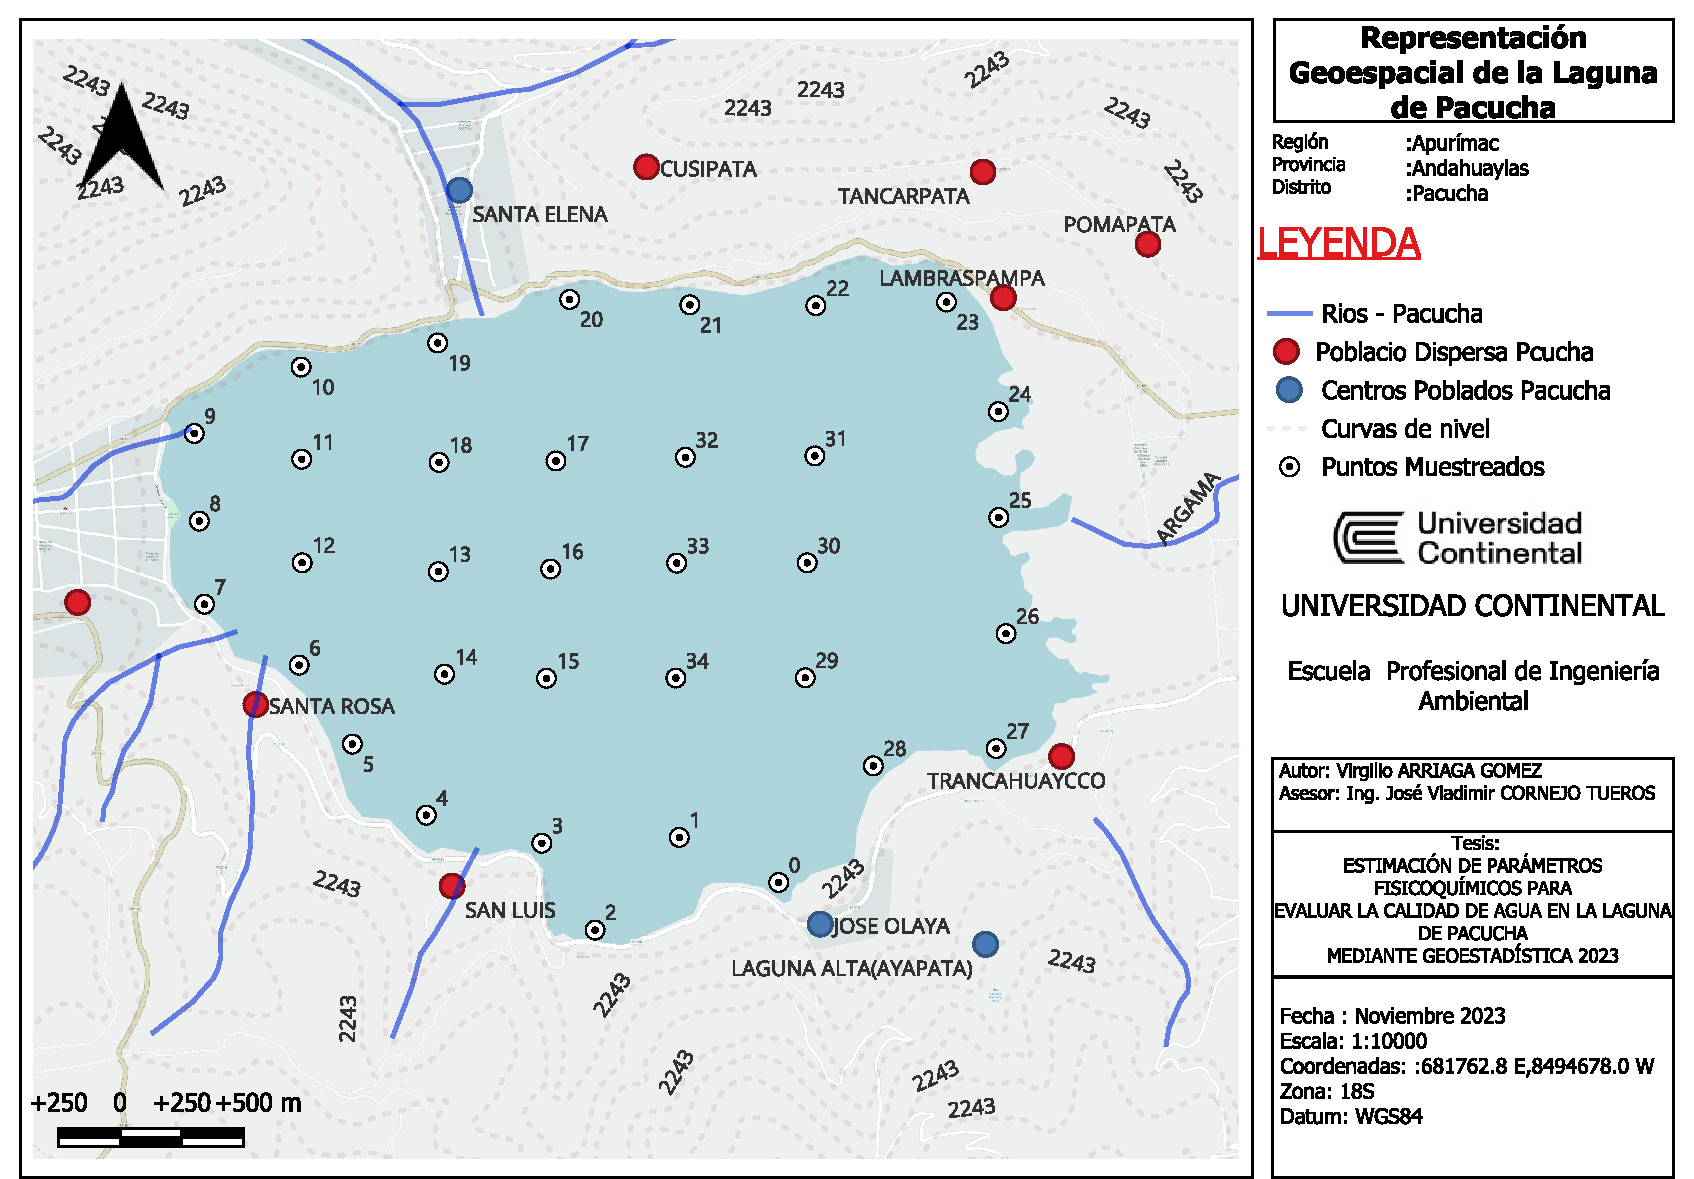
\includegraphics[width=0.9\linewidth]{Capitulos/GEOESTADICTICA_PACUCHA.pdf} 
        \caption{Mapa de la Laguna de Pacucha} % Agrega un título a la imagen.
    \end{figure}
\end{landscape}



\chapter{RESULTADOS Y DISCUSIÓN}

En el presente estudio, los análisis exploratorios, el análisis variográfico y la estimación mediante Kriging ordinario se llevarán a cabo utilizando el lenguaje de programación R y el entorno RStudio. Los algoritmos que se evaluarán serán adaptados de las herramientas proporcionadas por el paquete \texttt{RGEOSTAD} \cite{unknown}.

\begin{comment}
    

\section{Análisis exploratorio de datos}
En el contexto de esta investigación, y de acuerdo con los objetivos expuestos en el primer capítulo, se considerarán los siguientes parámetros: Oxígeno Disuelto (medido en mg/L), Temperatura (en grados Celsius) y pH. Estos fueron muestreados en la Laguna de Pacucha. Con el fin de llevar a cabo un análisis exhaustivo, se realizará un estudio estadístico para cada uno de estos parámetros. Además, se evaluará la idoneidad de un análisis bivariado, basado en la existencia y naturaleza de las correlaciones que puedan identificarse entre estos parámetros. Este enfoque nos permitirá comprender mejor las relaciones dinámicas y las interdependencias dentro del ecosistema acuático de la Laguna de Pacucha.

\subsection{Análisis estadístico univariado}
La Tabla \ref{my-label1} presenta un conjunto de datos fisicoquímicos obtenidos de la Laguna de Pacucha. Las muestras recogidas incluyen mediciones de temperatura (en grados Celsius), pH y oxígeno disuelto (en mg/L), los cuales son esenciales para un análisis exploratorio exhaustivo. Estos datos son fundamentales para la elaboración subsecuente de variogramas, que contribuirán significativamente a la consecución de los objetivos planteados en esta tesis: la estimación precisa de los parámetros fisicoquímicos que determinan la calidad del agua de la Laguna de Pacucha. El análisis geoestadístico permitirá identificar y modelar la variabilidad espacial de estos parámetros críticos, proporcionando así una comprensión más profunda de las condiciones ambientales del cuerpo de agua en estudio.


\begin{table}[!htb]
\centering
\caption{Datos de Temperatura, pH y Oxígeno Disuelto en el entorno de la Laguna de Pacucha}
\label{my-label1}
\small % Aplica un tamaño de fuente pequeño a toda la tabla
\setlength{\tabcolsep}{4pt} % Ajusta el espacio entre columnas
\renewcommand{\arraystretch}{0.9} % Ajusta el espacio entre filas
\begin{tabular}{@{}cccccc@{}}
\toprule
N°& X & Y & Temperatura (\textdegree{}C) & pH & Oxígeno Disuelto (mg/L) \\ \midrule
1 & 682370.9 & 8493381 & 18.62 & 8.74 & 5.29 \\
2 & 681968.2 & 8493564 & 18.62 & 8.64 & 5.08 \\
3 & 681626.5 & 8493188 & 18.63 & 8.64 & 5.03 \\
4 & 681410.7 & 8493540 & 18.69 & 8.67 & 5.28 \\
5 & 680942.6 & 8493654 & 18.73 & 8.69 & 5.30 \\
6 & 680642.8 & 8493942 & 18.74 & 8.66 & 5.27 \\
7 & 680426.7 & 8494262 & 18.90 & 8.70 & 5.39 \\
8 & 680043.0 & 8494509 & 18.92 & 8.73 & 5.12 \\
9 & 680022.2 & 8494846 & 18.95 & 8.68 & 5.17 \\
10 & 680001.5 & 8495201 & 18.98 & 8.73 & 5.58 \\
11 & 680435.0 & 8495471 & 19.08 & 8.73 & 5.64 \\
12 & 680437.3 & 8495097 & 19.10 & 8.72 & 5.69 \\
13 & 680438.9 & 8494677 & 19.01 & 8.72 & 5.74 \\
14 & 680991.1 & 8494641 & 19.01 & 8.71 & 5.91 \\
15 & 681016.2 & 8494226 & 18.85 & 8.70 & 5.90 \\
16 & 681429.4 & 8494209 & 18.82 & 8.68 & 5.92 \\
17 & 681446.3 & 8494652 & 18.90 & 8.70 & 5.91 \\
18 & 681468.0 & 8495090 & 19.12 & 8.68 & 6.07 \\
19 & 680994.2 & 8495084 & 19.26 & 8.72 & 6.18 \\
20 & 680988.5 & 8495568 & 19.26 & 8.72 & 6.29 \\
21 & 681523.6 & 8495745 & 19.22 & 8.74 & 6.52 \\
22 & 682011.0 & 8495723 & 19.20 & 8.70 & 6.45 \\
23 & 682521.8 & 8495719 & 19.18 & 8.70 & 6.28 \\
24 & 683051.2 & 8495734 & 19.22 & 8.68 & 6.33 \\
25 & 683261.6 & 8495290 & 19.25 & 8.69 & 6.49 \\
26 & 683263.4 & 8494861 & 19.34 & 8.69 & 6.62 \\
27 & 683292.6 & 8494390 & 19.23 & 8.66 & 6.65 \\
28 & 683252.4 & 8493924 & 19.22 & 8.67 & 6.52 \\
29 & 682755.0 & 8493854 & 19.24 & 8.66 & 6.62 \\
30 & 682478.8 & 8494211 & 19.19 & 8.68 & 6.51 \\
31 & 682486.6 & 8494677 & 19.37 & 8.69 & 6.54 \\
32 & 682517.5 & 8495110 & 19.29 & 8.70 & 6.57 \\
33 & 681992.6 & 8495105 & 19.39 & 8.71 & 6.57 \\
34 & 681957.2 & 8494676 & 19.38 & 8.73 & 6.69 \\
35 & 681954.0 & 8494210 & 19.02 & 8.70 & 6.43 \\ \bottomrule
\end{tabular}
\end{table}

\subsubsection{Estadísticos Básicos de los parámetros}

La Tabla \ref{tab:combined_statistics} indica que hay 35 mediciones para cada parámetro, lo que sugiere un conjunto de datos consistente para el análisis estadístico.

\textbf{Temperatura:} Las temperaturas varían de 18.62 a 19.39 grados Celsius, con una mediana de 19.10 y una media ligeramente inferior de 19.0551 grados Celsius. La varianza y la desviación estándar son relativamente bajas, lo que indica poca dispersión alrededor de la media. La asimetría negativa sugiere una cola más pesada hacia los valores bajos, y la curtosis indica una distribución más puntiaguda que una distribución normal.

\textbf{Oxígeno Disuelto:} Los valores oscilan entre 5.03 y 6.69 mg/L. La mediana y la media están bastante cercanas, lo que podría indicar una distribución simétrica, aunque la asimetría negativa implica un ligero sesgo hacia valores más pequeños. La curtosis es menor que la de la temperatura, lo que indica una distribución menos puntiaguda.

\textbf{pH:} Hay una menor variación en el pH, con una varianza de solo 0.0007, lo que indica que los valores están muy agrupados alrededor de la media de 8.696. La asimetría y la curtosis sugieren una distribución ligeramente sesgada y más plana que una distribución normal.

Este análisis preliminar de las estadísticas descriptivas brinda una comprensión inicial de las condiciones fisicoquímicas de la Laguna de Pacucha. La relativa estabilidad en las mediciones de temperatura y pH, junto con la variabilidad moderada en el oxígeno disuelto, pueden indicar patrones interesantes para investigaciones más detalladas. Por ejemplo, el análisis geoestadístico puede utilizar estos datos para modelar la variabilidad espacial y temporal de la calidad del agua. Los variogramas podrían ser particularmente útiles para comprender la estructura de dependencia espacial de los datos, lo cual es esencial para la interpolación espacial y la estimación de parámetros a través de técnicas como el kriging. Una comprensión profunda de la evaluación de la calidad del agua en este caso se beneficiaría de un entendimiento integral de cómo estos parámetros interactúan entre sí y con el entorno de la laguna.

\begin{table}[!htb]
\centering
\caption{Estadísticos descriptivos para Temperatura, Oxígeno Disuelto y pH}
\label{tab:combined_statistics}
\begin{tabular}{lccc}
\toprule
 & Temperatura & Oxígeno Disuelto & pH  \\
Statistics & & & \\
\midrule
n & 35.0000 & 35.0000 & 35.0000 \\
Minimum & 18.6200 & 5.0300 & 8.6400 \\
1st. Quartile & 18.9000 & 5.4850 & 8.6800 \\
Median & 19.1000 & 6.0700 & 8.7000 \\
Mean & 19.0551 & 5.9871 & 8.6960 \\
3rd. Quartile & 19.2350 & 6.5150 & 8.7200 \\
Maximum & 19.3900 & 6.6900 & 8.7400 \\
Rank & 0.7700 & 1.6600 & 0.1000 \\
Interquartile Rank & 0.3350 & 1.0300 & 0.0400 \\
Variance & 0.0549 & 0.3091 & 0.0007 \\
Standard Deviation & 0.2343 & 0.5560 & 0.0267 \\
Variation Coeff. & 0.0123 & 0.0929 & 0.0031 \\
Skewness & -0.4472 & -0.3476 & -0.2491 \\
Kurtosis & 2.0411 & 1.6411 & 2.3947 \\
\bottomrule
\end{tabular}
\end{table}

\subsubsection{Histogramas y Boxplot de la Temperatura}

En la Figura \ref{fig:enter-label1}  muestra el histograma y el diagrama de caja correspondiente a las lecturas de temperatura tomadas en la Laguna de Pacucha. El histograma indica que el rango de temperaturas que ocurre con mayor frecuencia está entre 19.2 y 19.3 °C, lo que representa el 25.7\% del total de observaciones, sugiriendo una concentración de valores dentro de este intervalo. Por el contrario, los intervalos de temperatura de 18.7 a 18.9 °C son los menos frecuentes, cada uno comprendiendo el 11.4\% de las observaciones, lo que implica una menor ocurrencia de estas temperaturas en la laguna.

Además, el diagrama de caja superpuesto presenta una representación visual de la distribución de los datos, enfatizando las temperaturas media y mediana. La línea azul de la mediana sugiere que la mitad de las mediciones están por debajo de esta línea, mientras que la otra mitad está por encima. La línea roja punteada de la media indica la temperatura promedio, y su proximidad a la mediana sugiere una distribución relativamente simétrica de los datos. La ligera discrepancia entre la media y la mediana podría indicar una asimetría sutil en la distribución de las temperaturas.

Además, el diagrama de caja ilustra que la mayoría de las mediciones de temperatura se agrupan alrededor de la mediana, con algunos valores atípicos que se extienden hacia el rango superior. Esta tendencia refleja la variabilidad térmica en la Laguna de Pacucha y ofrece una base sólida para futuros análisis geoestadísticos destinados a esclarecer las dinámicas del ecosistema acuático.

\begin{figure}[!htb]
    \centering
    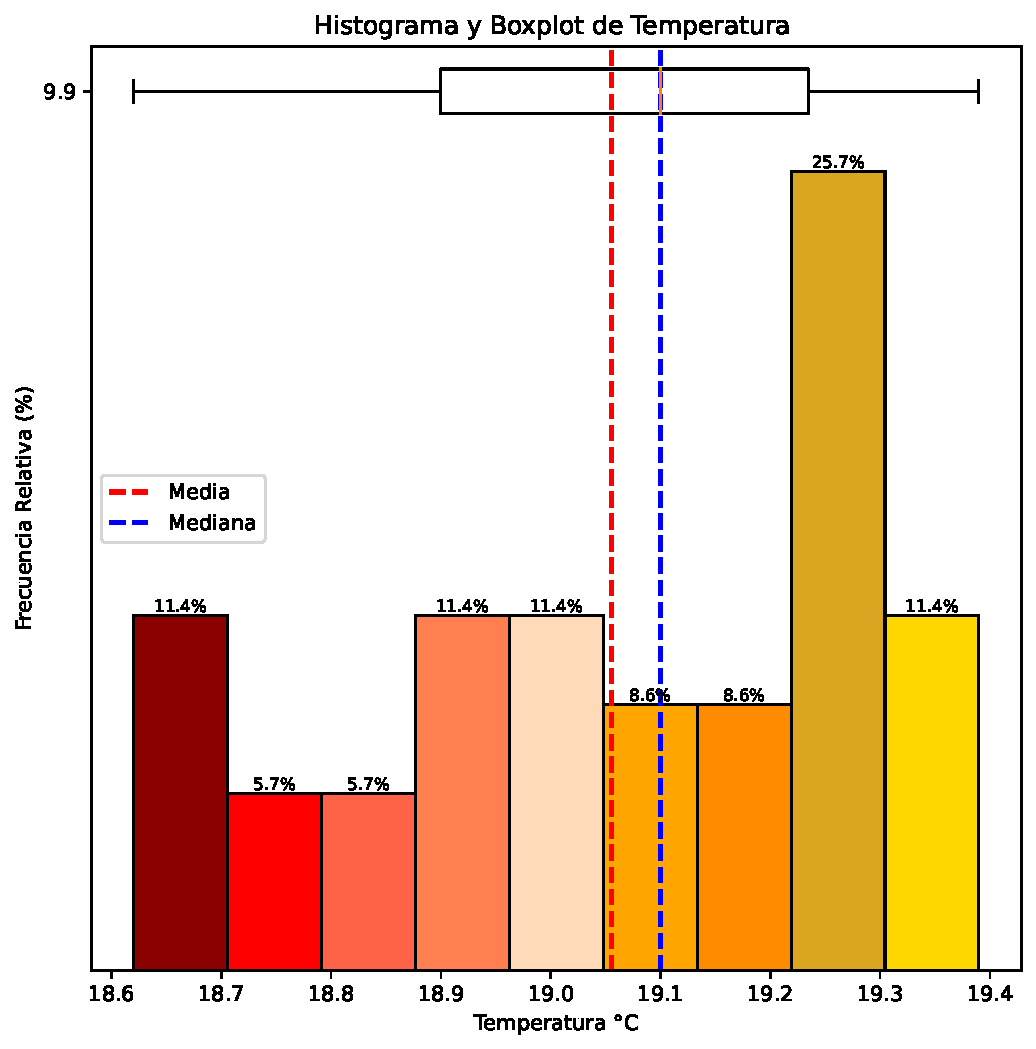
\includegraphics[width=0.5\linewidth]{Figuras_AED/Histograma_Temperatura.pdf}
    \caption{Frecuencia y Rango de la Temperatura, Perspectiva Gráfica}
    \label{fig:enter-label1}
\end{figure}

\subsubsection{Histogramas y Boxplot del Oxígeno Disuelto}

La Figura \ref{fig:enter-label2}  presenta un gráfico compuesto que integra un histograma y un diagrama de caja para ilustrar las mediciones de oxígeno disuelto en mg/L. El histograma, representado por barras verticales, delinea la frecuencia relativa de los distintos rangos de concentración de oxígeno disuelto. Es evidente que la frecuencia relativa más alta, aproximadamente el 28.6\%, se observa en el rango entre 6.5 y 6.7 mg/L, lo que implica que este es el rango de concentración más común en el conjunto de datos considerado.

Superpuesto en el histograma, el diagrama de caja ofrece un resumen sucinto de la distribución de los datos. Resalta la mediana (línea azul) y la media (línea roja punteada) de las concentraciones de oxígeno disuelto. La mediana está posicionada cerca del centro del rango de datos, lo que indica que la mitad de las mediciones caen por debajo de este valor y la otra mitad por encima. La media está ligeramente sesgada hacia el rango de mayor concentración, lo que puede sugerir una distribución asimétrica con una cola hacia concentraciones más altas de oxígeno disuelto.

Las barras del histograma están coloreadas y la frecuencia relativa de cada barra se muestra de manera conspicua en porcentajes. El gráfico en su conjunto proporciona una visión integral de la variabilidad de las mediciones de oxígeno disuelto en la muestra analizada. Notablemente, los valores atípicos se identificarían como puntos fuera de los ``bigotes'', o las líneas horizontales que se extienden desde la caja central del diagrama de caja. En este caso, no se aprecian valores atípicos.

\begin{figure}[!htb]
    \centering
    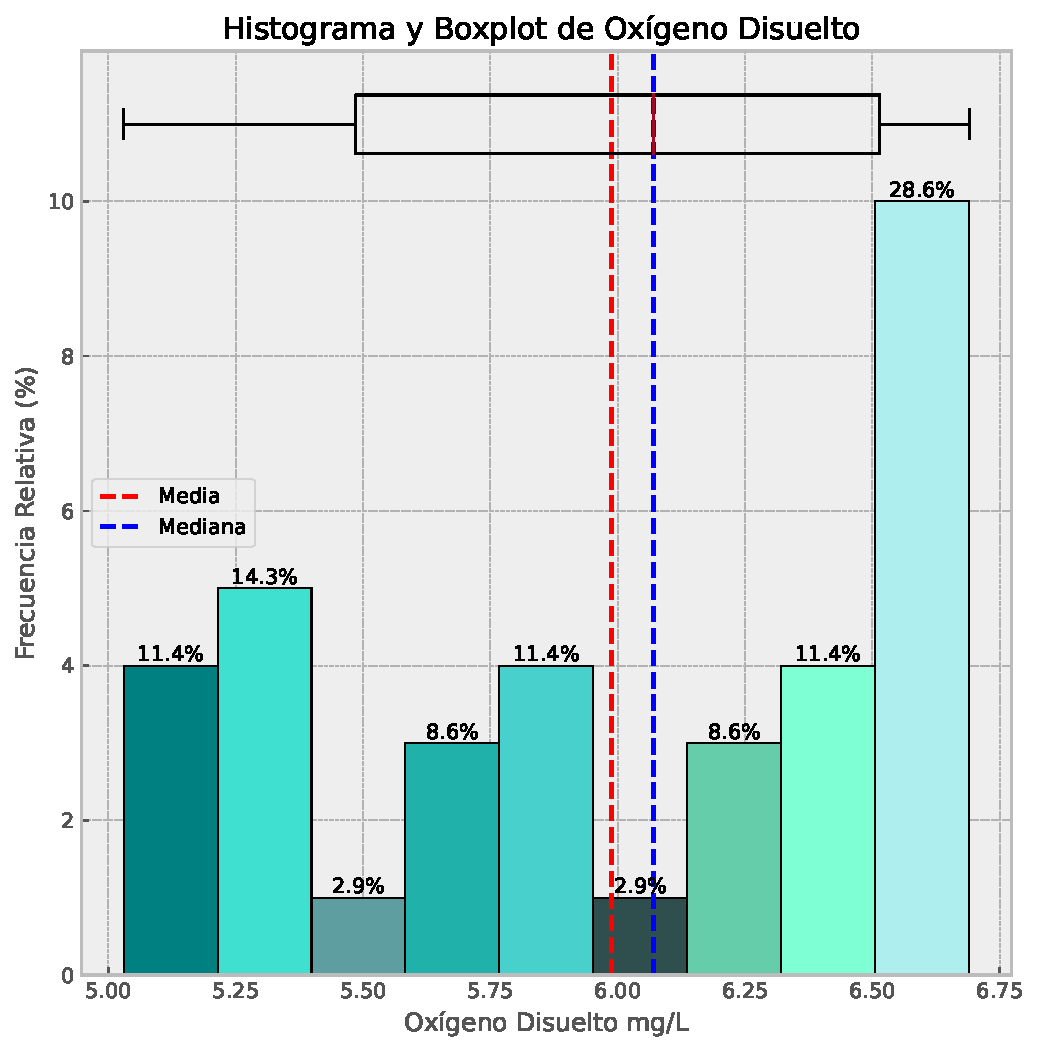
\includegraphics[width=0.5\linewidth]{Figuras_AED/Histograma_Oxigeno_Disuelto.pdf}
    \caption{Frecuencia y Rango del Oxígeno Disuelto, Perspectiva Gráfica}
    \label{fig:enter-label2}
\end{figure}

\subsubsection{Histogramas y Boxplot del pH}
En la Figura \ref{fig:enter-label4} se observa una representación gráfica de los niveles de pH medidos en la Laguna de Pacucha, donde se está realizando la investigación actual. El histograma muestra la frecuencia relativa de los valores de pH observados, con barras verticales que ilustran la distribución de estos valores dentro del conjunto de datos. Es notable que el valor de pH más común, representado por la barra más alta, corresponde aproximadamente al 29\% de las mediciones, alrededor de 8.70. Este pico indica una tendencia de los valores de pH a agruparse alrededor de este punto central en la Laguna de Pacucha.

En contraste, las frecuencias relativas en los rangos de pH más bajos y más altos, visibles en los extremos del histograma, son considerablemente menos comunes, con porcentajes del 2.9\% y 17.1\%, respectivamente. Esto sugiere que los valores extremos de pH son menos prevalentes en la laguna, lo cual es crucial para analizar el equilibrio ecológico y la calidad del agua en la Laguna de Pacucha.

El diagrama de caja superpuesto ofrece una visión concisa de la dispersión de los datos, con la mediana (línea roja) y la media (línea azul punteada) ubicadas cerca una de la otra, lo que sugiere una distribución simétrica y equilibrada de los valores de pH en la laguna. La ausencia de valores atípicos, indicada por la falta de puntos más allá de los bordes del diagrama de caja, refuerza la idea de que los valores de pH en la Laguna de Pacucha se mantienen dentro de un rango consistente, sin fluctuaciones extremas que podrían señalar condiciones ambientales inusuales.

\begin{figure} [!htb]
    \centering
    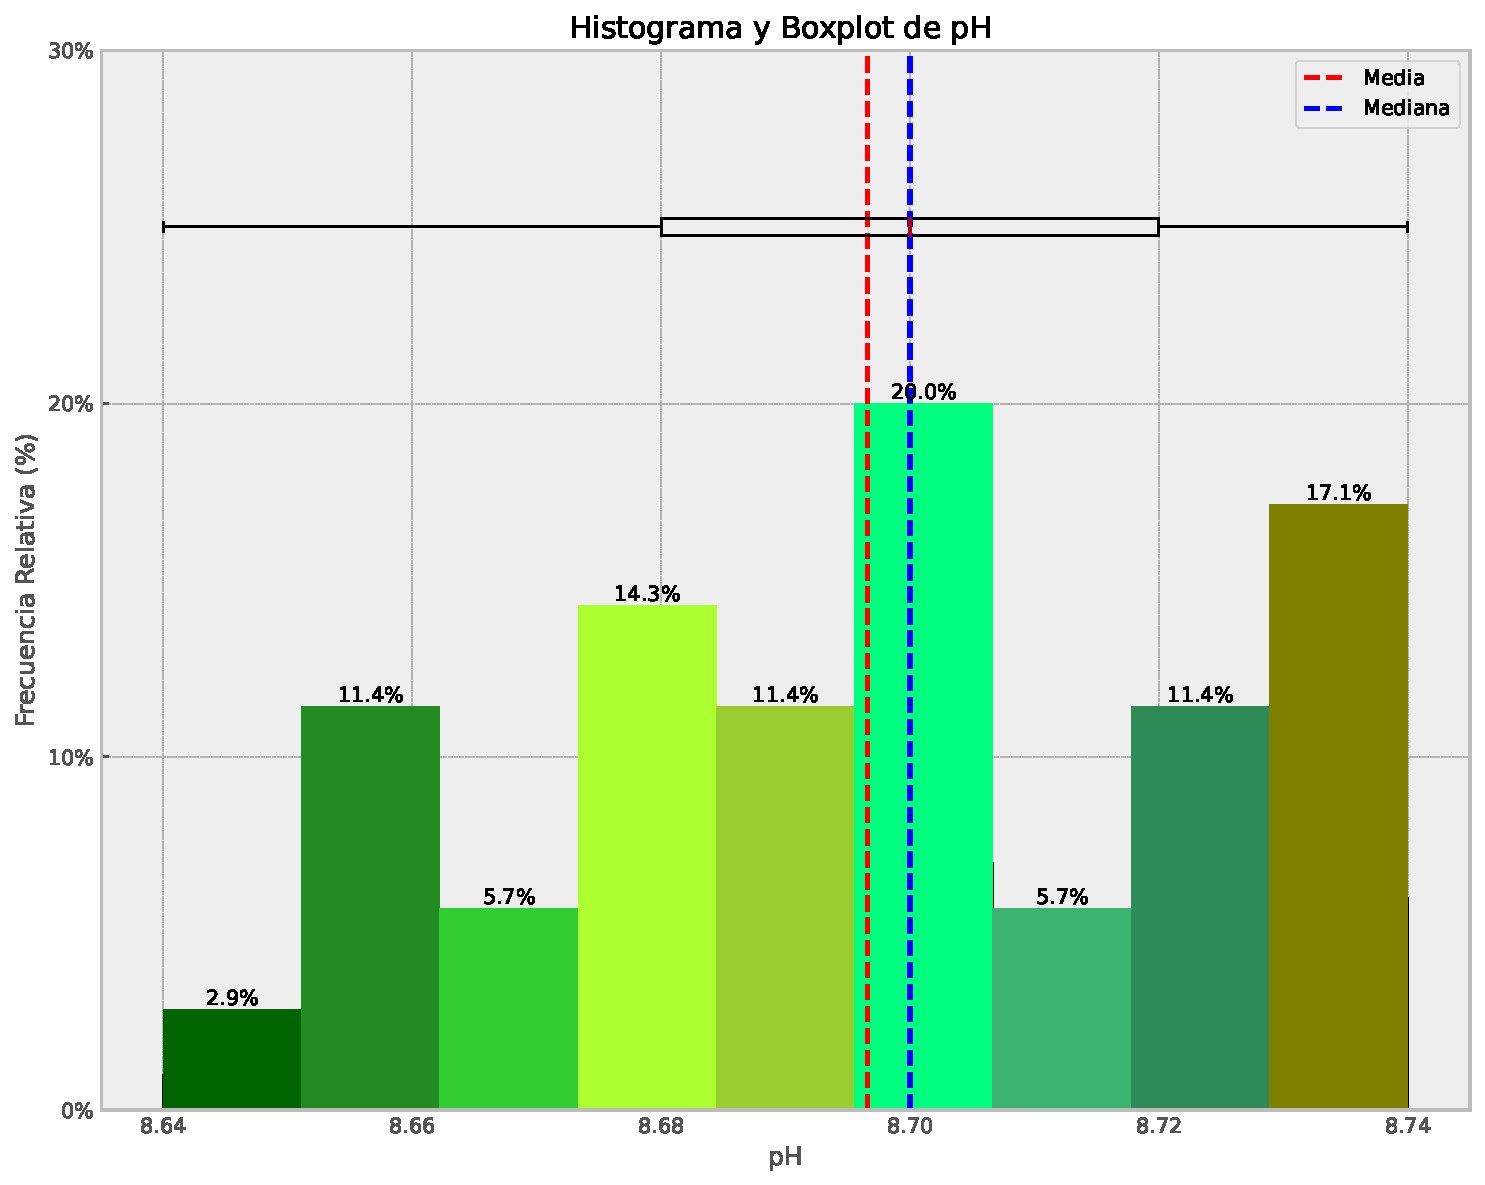
\includegraphics[width=0.5\linewidth]{Figuras_AED/Histograma_pH.pdf}
    \caption{Frecuencia y Rango del pH, Perspectiva Gráfica}
    \label{fig:enter-label4}
\end{figure}

\subsection{Análisis estadístico bivariado}


\begin{table}[!htb]
\centering 
\caption{Coeficientes de correlación entre las variables fisicoquímicas}

\label{tab:correlation}
\begin{tabular}{@{}lccc@{}}
\toprule
Método de Correlación & OD y pH & Temperatura y pH & OD y Temperatura \\ \midrule
Pearson & 0.07103201 & 0.2270671 & 0.8851791 \\
Spearman & 0.01681203 & 0.1692979 & 0.8788899 \\
Kendall & -0.0230761 & 0.1245725 & 0.6972033 \\ \bottomrule
\end{tabular}
\end{table}

\subsubsection{Regresión Lineal}

El Gráfico \ref{fig:enter-matriz_regre} ofrece una visualización completa de tres parámetros fisicoquímicos críticos: Temperatura, pH y Oxígeno Disuelto, medidos en la Laguna de Pacucha. La matriz de gráficos incluye histogramas que describen las distribuciones individuales de cada variable a lo largo de la diagonal principal y gráficos de dispersión que ilustran las relaciones bivariadas entre las variables en las celdas fuera de la diagonal.

En cuanto a la Temperatura y el Oxígeno Disuelto, la ecuación de regresión lineal viene dada por \( y = 2.10x - 34.04 \), con un coeficiente de correlación de Pearson (r) de 0.89 y un valor de \( R^2 \) de 0.78. Estos valores altos indican una fuerte correlación positiva, lo que sugiere que un aumento en la temperatura está asociado con un incremento en los niveles de oxígeno disuelto. Esta relación es particularmente relevante para la variografía y el análisis geoestadístico, ya que la correlación significativa puede ser un indicador confiable para la predicción espacial del oxígeno disuelto basada en la temperatura.

Para la Temperatura y el pH, la ecuación de regresión se da por \( y = 0.02x + 8.22 \), con un valor de r de 0.23 y un valor de \( R^2 \) de 0.05. Aunque hay una correlación positiva, es relativamente débil, lo que indica que la temperatura no es un fuerte predictor del pH. Desde una perspectiva geoestadística, esta relación puede no ser útil para la predicción espacial sin una exploración adicional de posibles relaciones no lineales o la inclusión de otras variables.

Finalmente, la relación entre el pH y el Oxígeno Disuelto se describe con la ecuación \( y = 1.54x + 7.40 \) con un valor de \( r \) de -0.02 y un valor de \( R^2 \) de 0.01. La correlación es prácticamente inexistente, lo que indica que no hay una relación lineal directa entre estas dos variables. Para un análisis variográfico, esta falta de correlación sugiere que el pH y el Oxígeno Disuelto se distribuyen independientemente el uno del otro y, por lo tanto, cada uno debe ser modelado sin considerar al otro como un predictor directo en el contexto geoestadístico de la Laguna de Pacucha.

Estos resultados proporcionan una base sólida para la selección de modelos en el análisis geoestadístico y enfatizan la importancia de considerar la fuerza y la forma de las correlaciones al aplicar la variografía para entender la distribución espacial de las variables fisicoquímicas en un ecosistema acuático.


\begin{figure}[!htb]
    \centering
    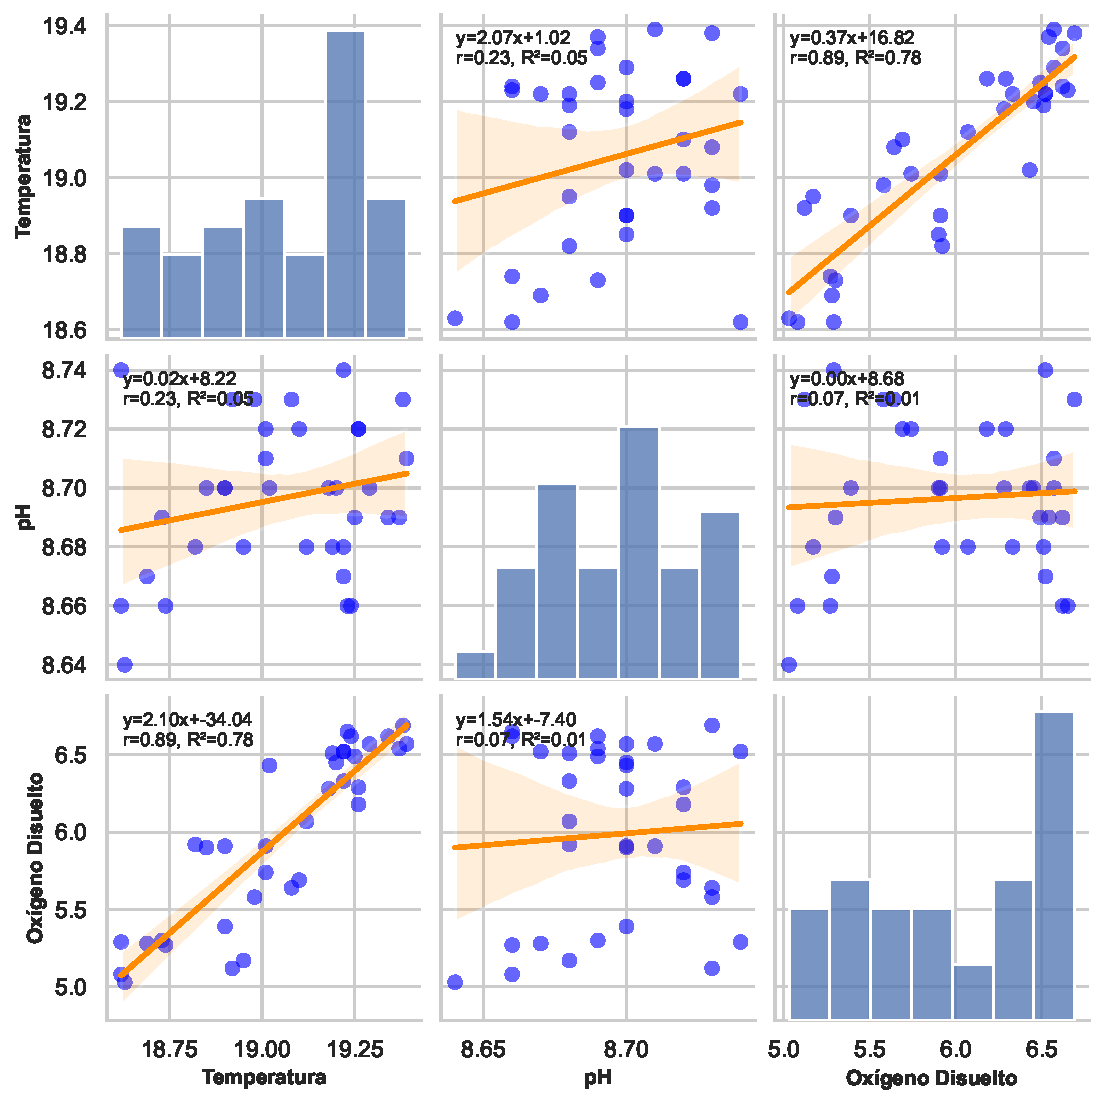
\includegraphics[width=1\linewidth]{Figuras_AED/matriz_de_pares_regresion_colores_fuertes.pdf}
    \caption{Matriz de regresión de los parámetros fisicoquímicos en estudio }
    \label{fig:enter-matriz_regre}
\end{figure}

\subsubsection{Análisis de la regresión lineal del Oxígeno disuelto y la Temperatura}

\begin{table}[ht]
\centering
\caption{Análisis estadístico de los residuos para la regresión lineal entre Oxígeno Disuelto y Temperatura}
\label{tab:residual_statistics}
\begin{tabular}{@{}lc@{}}
\toprule
Estadística & Valor \\
\midrule
Número de muestras (n) & 35 \\
Mínimo & -0.5963 \\
Primer cuartil & -0.1240 \\
Mediana & 0.0177 \\
Media & 0.0000 \\
Tercer cuartil & 0.1866 \\
Máximo & 0.5167 \\
Rango & 1.1130 \\
Rango intercuartílico & 0.3106 \\
Varianza & 0.0669 \\
Desviación estándar & 0.2587 \\
Coeficiente de variación (CV) & $1.082173 \times 10^{16}$ \\
Asimetría (Skewness) & -0.4090 \\
Curtosis & 3.0217 \\
\bottomrule
\end{tabular}
\end{table}

Esta Tabla \ref{tab:residual_statistics} presenta las estadísticas descriptivas de los residuos derivados del análisis de regresión lineal entre el Oxígeno Disuelto y la Temperatura. Cada fila de la tabla representa una medida estadística de los residuos. La media de los residuos es cero, lo cual es una característica común de la regresión lineal y sugiere que la suma de residuos positivos y negativos está equilibrada. La desviación estándar y la varianza proporcionan una indicación de la dispersión de los residuos alrededor de la media, mientras que la asimetría y la curtosis ofrecen información sobre la forma de la distribución de los residuos. Un valor de curtosis mayor que 3 (como en este caso, 3.0217) indica una distribución con colas más pesadas que una distribución normal, lo que podría sugerir la presencia de valores atípicos. Sin embargo, el Coeficiente de Variación (CV) parece ser extremadamente alto debido a que la media de los residuos es cero, y este valor puede no ser informativo en este contexto y puede requerir una interpretación cuidadosa o exclusión si no es relevante para el análisis.

\begin{figure} [!htb]
    \centering
    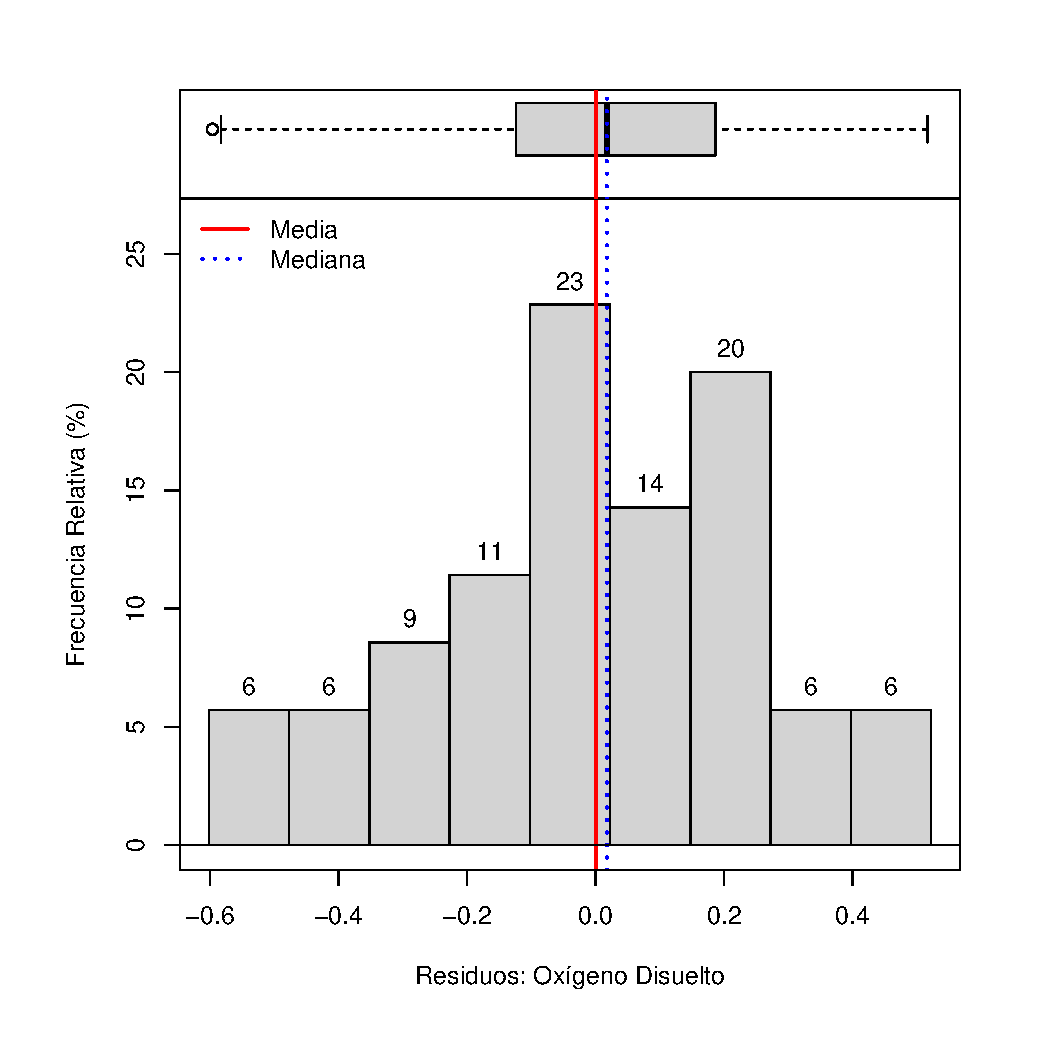
\includegraphics[width=0.5\linewidth]{Figuras_AED/OD_Residual_HistBoxPlot.pdf}
    \caption{Histograma y Boxplot de los residuos}
    \label{fig:enter-labelod}
\end{figure}

La Figura \ref{fig:enter-labelod} muestra un histograma de los residuos resultantes de un análisis de regresión lineal entre el Oxígeno Disuelto y la Temperatura. Los residuos son las diferencias entre los valores observados y los valores predichos por el modelo de regresión. En un buen modelo de regresión lineal, esperaríamos que los residuos se distribuyeran aproximadamente de manera normal alrededor de cero, sin patrones claros y con una asimetría cercana a cero.

En el histograma, se puede observar que la línea roja sólida, que representa la media de los residuos, está ubicada en cero. Esto es de esperar, ya que la suma de residuos positivos y negativos en un modelo de regresión lineal es cero por diseño. La línea roja punteada, que representa la mediana, también está cerca de cero, lo que sugiere que no hay una asimetría significativa en la distribución de los residuos. Sin embargo, un entendimiento más completo de la normalidad de los residuos sería proporcionado al analizar la simetría y la curtosis, junto con una prueba formal de normalidad (como la prueba de Kolmogorov-Smirnov y Anderson-Darling ).

La validez del modelo de regresión lineal se determina no solo por la normalidad de los residuos, sino también por la homocedasticidad, que se refiere a la varianza constante de los residuos a lo largo del rango de valores predichos. Aunque el histograma no muestra signos obvios de heterocedasticidad, sería necesario inspeccionar visualmente un gráfico de dispersión de residuos contra valores predichos para confirmar esto.

Además, la ausencia de barras extremadamente altas o bajas en el histograma sugiere que no hay valores atípicos significativos que podrían influir en la regresión. La presencia de valores atípicos podría tener un impacto sustancial en la pendiente y la intersección de la línea de regresión.

En resumen, el histograma aporta evidencia preliminar que apoya la aplicabilidad del modelo de regresión lineal a este conjunto de datos. Sin embargo, son necesarios estudios adicionales para verificar todas las hipótesis inherentes al modelo de regresión lineal y para establecer su validez. Estas verificaciones incluyen la realización de pruebas para confirmar la distribución normal de los residuos, la evaluación de la homocedasticidad de la varianza residual a través del espectro de valores predichos y la detección de cualquier punto anómalo o influyente.

\subsubsection{Ajuste de una distribución normal de los residuos}

La Figura \ref{fig:enter-labelRES} presenta cuatro gráficos esenciales para determinar la adecuación de la distribución normal como modelo para los residuos. En el histograma emparejado con la curva de densidad, la curva real coincide casi con las barras del histograma, lo que indica un ajuste adecuado. El gráfico Q-Q demuestra que los cuantiles empíricos siguen el patrón de los cuantiles teóricos, validando aún más la suposición de normalidad. Los gráficos CDF y P-P ilustran una alineación cercana entre las distribuciones y probabilidades acumulativas empíricas y teóricas, respectivamente, lo que implica que la distribución real de los datos se asemeja estrechamente a la distribución normal esperada.


\begin{figure} [!htb]
    \centering
    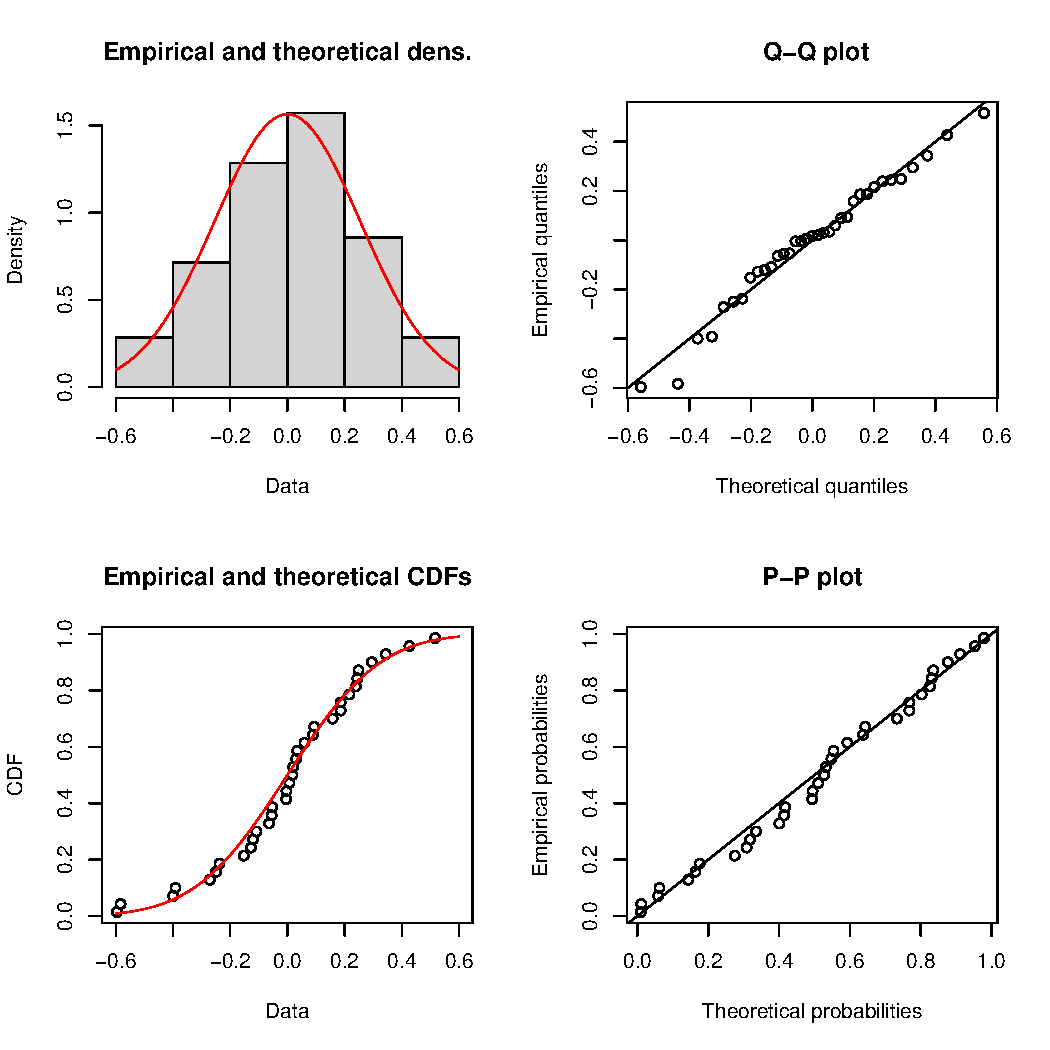
\includegraphics[width=0.9\linewidth]{Figuras_AED/OD_Residual_Fit.pdf}
    \caption{Ajuste de una distribución normal de los residuos}
    \label{fig:enter-labelRES}
\end{figure}

\subsubsection{Pruebas de hipótesis de normalidad}

La Tabla \ref{tab:goodness_of_fit_tests} delinea la prueba estadística empleada, el valor umbral denominado ``Nivel de Significancia'', por debajo del cual se descartaría la hipótesis nula (en este caso, una distribución normal), el ``P-valor'' obtenido de la prueba y la ``Decisión Estadística'', que indica si la hipótesis nula ha sido rechazada o no basándose en el P-valor y el nivel de significancia. Para ambas técnicas, el P-valor excede el nivel de significancia de 0.05, indicando que no hay evidencia suficiente para refutar la hipótesis nula de la normalidad de los datos.

\begin{table}[ht]
\centering
\caption{Resultados de las pruebas de bondad de ajuste para la normalidad}
\label{tab:goodness_of_fit_tests}
\begin{tabular}{@{}lccc@{}}
\toprule
Método & Nivel de Significancia & P-valor & Decisión Estadística \\
\midrule
Kolmogorov-Smirnov & 0.05 & 0.9197 & No rechazo \( H_0 \) \\
Anderson-Darling & 0.05 & 0.9361 & No rechazo \( H_0 \) \\
\bottomrule
\end{tabular}
\end{table}

\subsubsection{Análisis bivariado entre los residuos de un modelo de regresión lineal y la variable  Oxígeno Disuelto}
\begin{enumerate}
    \item \textbf{Prueba de Homocedasticidad u Homogeneidad de Varianzas}


\begin{table}[H]
\centering
\caption{Resultados de la Prueba de Breusch-Pagan para Homocedasticidad}
\begin{tabular}{lc}
\hline
\textbf{Estadístico} & \textbf{Valor} \\
\hline
Estadístico de Prueba & 0.835 \\
Valor-p & 0.361 \\
\hline
\end{tabular}
\label{tab:breusch_pagan_test}
\end{table}

En el campo del análisis de regresión, la suposición de homocedasticidad de los residuos es esencial para garantizar la precisión de varias inferencias estadísticas. La prueba de Breusch-Pagan es un método ampliamente utilizado para examinar esta suposición. Esta prueba plantea la hipótesis nula de que los errores son homocedásticos, lo que implica que sus varianzas son constantes, mientras que la hipótesis alternativa propone que los errores son heterocedásticos, lo que implica que sus varianzas no son constantes.

Los resultados de la prueba de Breusch-Pagan en este estudio muestran un estadístico de prueba de 0.835 y un valor-p de 0.361, como se indica en la Tabla \ref{tab:breusch_pagan_test} . El estadístico de prueba por sí solo es insuficiente para determinar la aceptación o el rechazo de la hipótesis nula; su interpretación depende del valor-p asociado. En este caso, el valor-p supera el umbral comúnmente aceptado de 0.05, lo que indica que no hay evidencia suficiente para rechazar la hipótesis nula de homocedasticidad.

Por lo tanto, basándose en esta prueba, se puede inferir que no hay evidencia estadísticamente significativa de heterocedasticidad en los residuos del modelo de regresión. Esta conclusión refuerza la validez de ciertas inferencias estadísticas derivadas del modelo, como la fiabilidad de los intervalos de confianza y las pruebas de hipótesis para los coeficientes de regresión.

    \item \textbf{Prueba de no linealidad}
\end{enumerate}

\begin{table}[H]
\centering
\caption{Resultados de la Prueba de Harvey-Collier para No Linealidad}
\begin{tabular}{lc}
\hline
\textbf{Aspecto} & \textbf{Resultado} \\
\hline
Estadístico de Prueba & -2.392 \\
Valor-p & 0.023 \\
\hline
\end{tabular}
\label{tab:harvey_collier_test}
\end{table}

La prueba de Harvey-Collier es una herramienta estadística utilizada para detectar la no linealidad en los residuos de un modelo de regresión. Esta prueba evalúa la hipótesis nula de que un modelo lineal es apropiado en contra de la hipótesis alternativa de que un modelo no lineal sería más adecuado.

En la Tabla \ref{tab:harvey_collier_test} , los resultados de la prueba de Harvey-Collier indican un estadístico de prueba aproximado de -2.392 y un valor-p de aproximadamente 0.023. El estadístico de prueba negativo proporciona evidencia en contra de la hipótesis nula, y el valor-p, al ser menor que el umbral comúnmente aceptado de 0.05, refuerza esta evidencia. En consecuencia, se rechaza la hipótesis nula, sugiriendo que hay evidencia estadísticamente significativa de no linealidad en los residuos del modelo.

Las implicaciones de estos hallazgos son que un modelo no lineal podría ser más adecuado para capturar la relación entre las variables de estudio. La presencia de no linealidad en los residuos sugiere que el modelo lineal actual puede no ser la mejor representación de la relación entre las variables, lo que podría motivar la exploración de modelos alternativos que incluyan términos no lineales o transformaciones de las variables.

\section{Análisis exploratorio de datos}

En esta investigación se analizaron los parámetros Oxígeno Disuelto (mg/L), Temperatura (°C) y pH en la Laguna de Pacucha. Se realizó un estudio estadístico univariado y bivariado para comprender las relaciones e interdependencias dentro del ecosistema acuático.

\subsection{Análisis estadístico univariado}

La Tabla \ref{my-label1} presenta los datos fisicoquímicos obtenidos de la Laguna de Pacucha. Estos datos son esenciales para elaborar variogramas y analizar la variabilidad espacial de los parámetros, lo cual es fundamental para la estimación precisa de la calidad del agua.

\begin{table}[!htb]
\centering
\caption{Datos de Temperatura, pH y Oxígeno Disuelto en el entorno de la Laguna de Pacucha}
\label{my-label1}
\small
\setlength{\tabcolsep}{4pt}
\renewcommand{\arraystretch}{0.9}
\begin{tabular}{@{}cccccc@{}}
\toprule
N° & X & Y & Temperatura (\textdegree{}C) & pH & Oxígeno Disuelto (mg/L) \ \midrule
1 & 682370.9 & 8493381 & 18.62 & 8.74 & 5.29 \
2 & 681968.2 & 8493564 & 18.62 & 8.64 & 5.08 \
... & ... & ... & ... & ... & ... \
35 & 681954.0 & 8494210 & 19.02 & 8.70 & 6.43 \ \bottomrule
\end{tabular}
\end{table}

\subsubsection{Estadísticos Básicos de los parámetros}

La Tabla \ref{tab
} muestra estadísticas descriptivas de los parámetros medidos.

\begin{table}[!htb]
\centering
\caption{Estadísticos descriptivos para Temperatura, Oxígeno Disuelto y pH}
\label{tab
}
\begin{tabular}{lccc}
\toprule
& Temperatura & Oxígeno Disuelto & pH \
\midrule
n & 35 & 35 & 35 \
Mínimo & 18.62 & 5.03 & 8.64 \
Mediana & 19.10 & 6.07 & 8.70 \
Media & 19.06 & 5.99 & 8.70 \
Máximo & 19.39 & 6.69 & 8.74 \
Desviación Estándar & 0.23 & 0.56 & 0.03 \
Asimetría & -0.45 & -0.35 & -0.25 \
Curtosis & 2.04 & 1.64 & 2.39 \
\bottomrule
\end{tabular}
\end{table}

\subsubsection{Histogramas y Boxplot}

\begin{figure}[!htb]
\centering
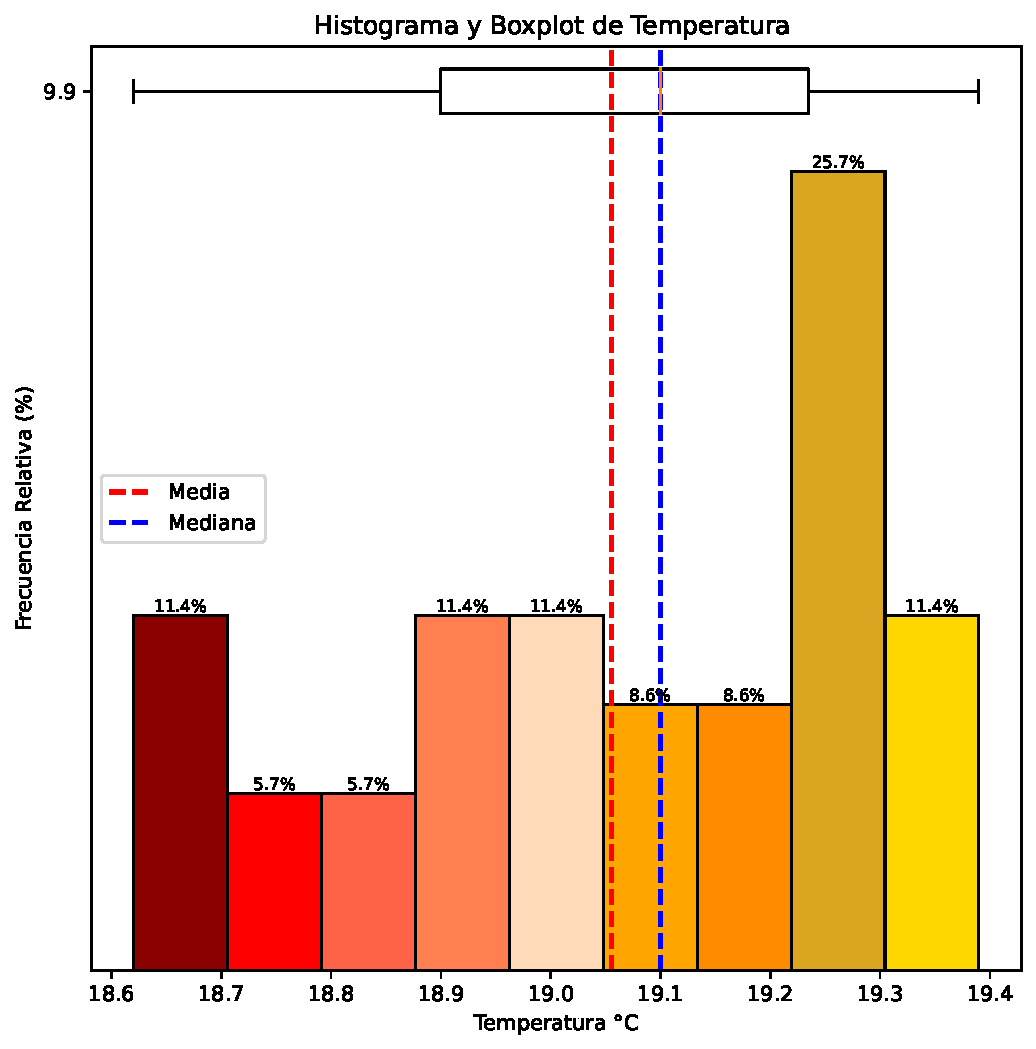
\includegraphics[width=0.5\linewidth]{Figuras_AED/Histograma_Temperatura.pdf}
\caption{Frecuencia y Rango de la Temperatura}
\label{fig
}
\end{figure}

La Figura \ref{fig
} muestra el histograma y boxplot de las temperaturas. La mayoría de las temperaturas se concentran entre 19.2 y 19.3 °C.

\begin{figure}[!htb]
\centering
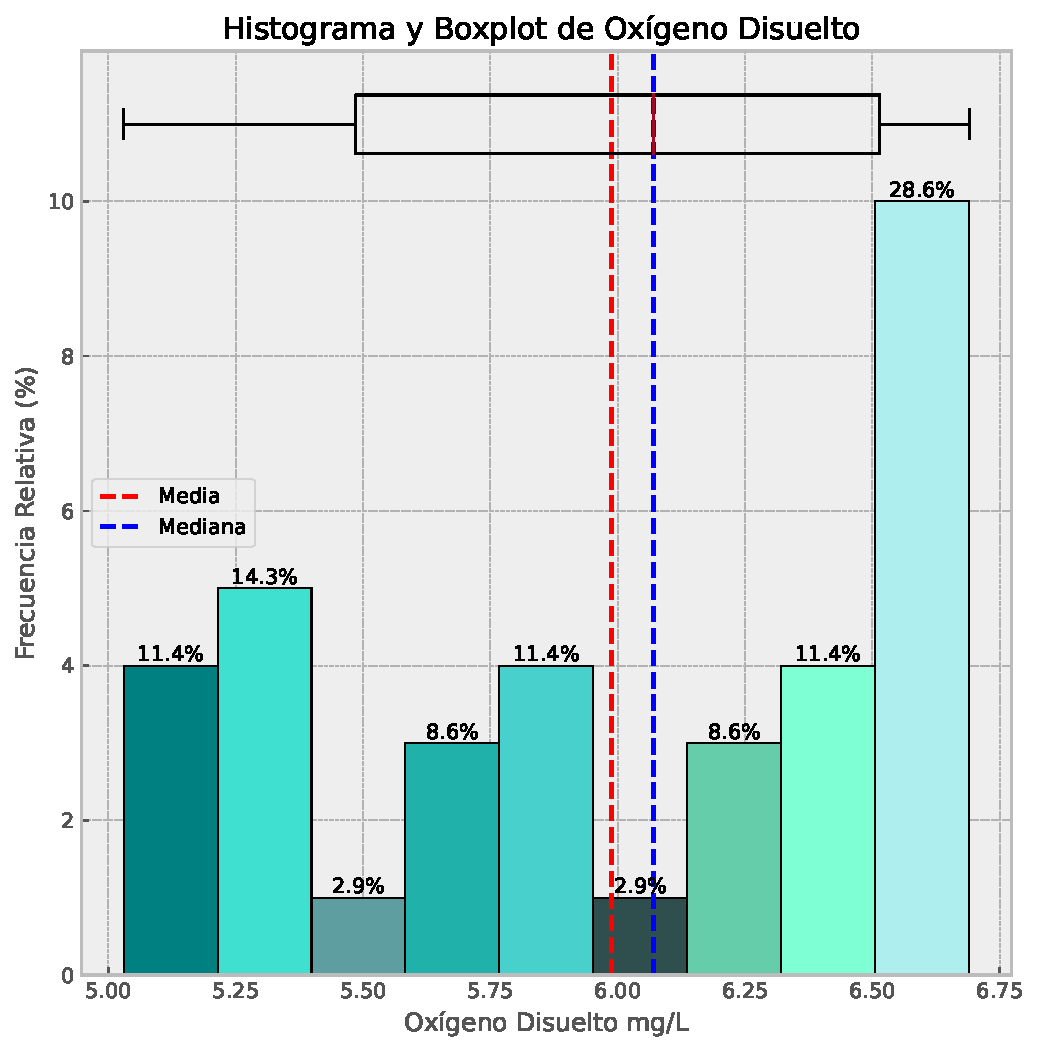
\includegraphics[width=0.5\linewidth]{Figuras_AED/Histograma_Oxigeno_Disuelto.pdf}
\caption{Frecuencia y Rango del Oxígeno Disuelto}
\label{fig
}
\end{figure}

La Figura \ref{fig
} ilustra las concentraciones de oxígeno disuelto, siendo 6.5-6.7 mg/L el rango más común.

\begin{figure}[!htb]
\centering
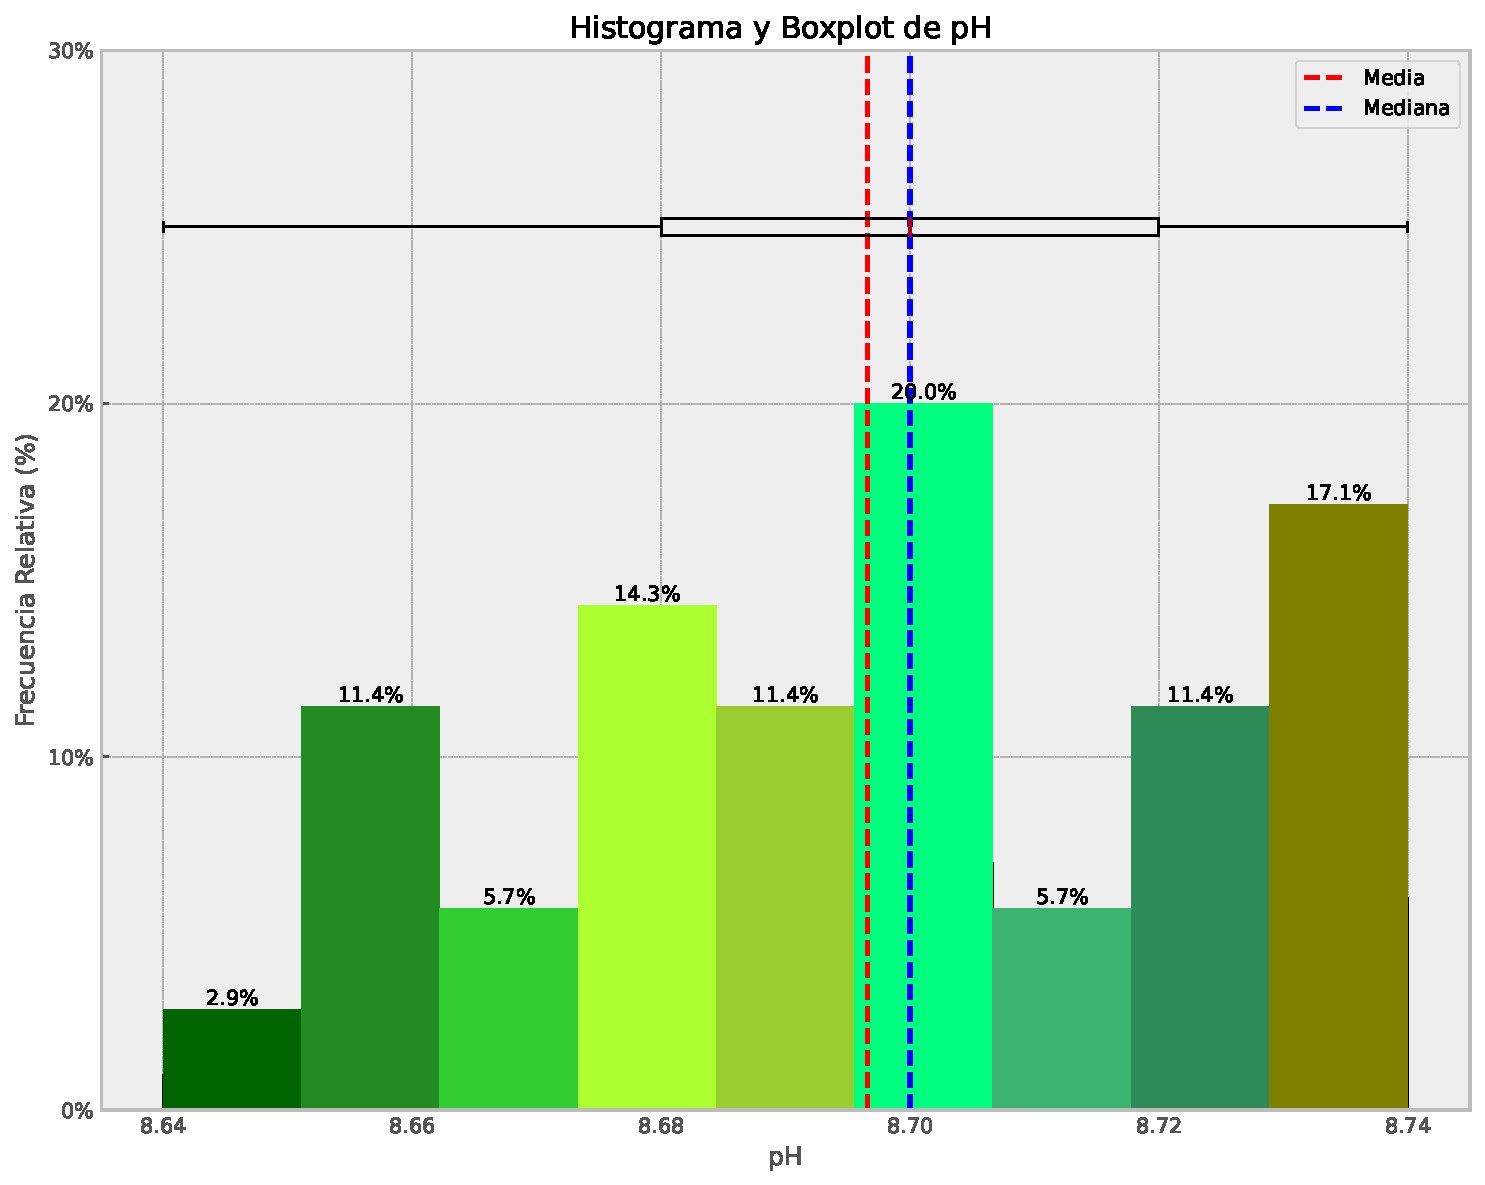
\includegraphics[width=0.5\linewidth]{Figuras_AED/Histograma_pH.pdf}
\caption{Frecuencia y Rango del pH}
\label{fig
}
\end{figure}

La Figura \ref{fig
} representa los valores de pH, concentrados alrededor de 8.70.

\subsection{Análisis estadístico bivariado}

\begin{table}[!htb]
\centering
\caption{Coeficientes de correlación entre las variables fisicoquímicas}
\label{tab
}
\begin{tabular}{@{}lccc@{}}
\toprule
Método & OD y pH & Temperatura y pH & OD y Temperatura \ \midrule
Pearson & 0.07 & 0.23 & 0.89 \
Spearman & 0.02 & 0.17 & 0.88 \
Kendall & -0.02 & 0.12 & 0.70 \ \bottomrule
\end{tabular}
\end{table}

\subsubsection{Regresión Lineal}

La Figura \ref{fig
} muestra la matriz de regresión de los parámetros fisicoquímicos. La temperatura y el oxígeno disuelto tienen una fuerte correlación positiva (r = 0.89).

\begin{figure}[!htb]
\centering
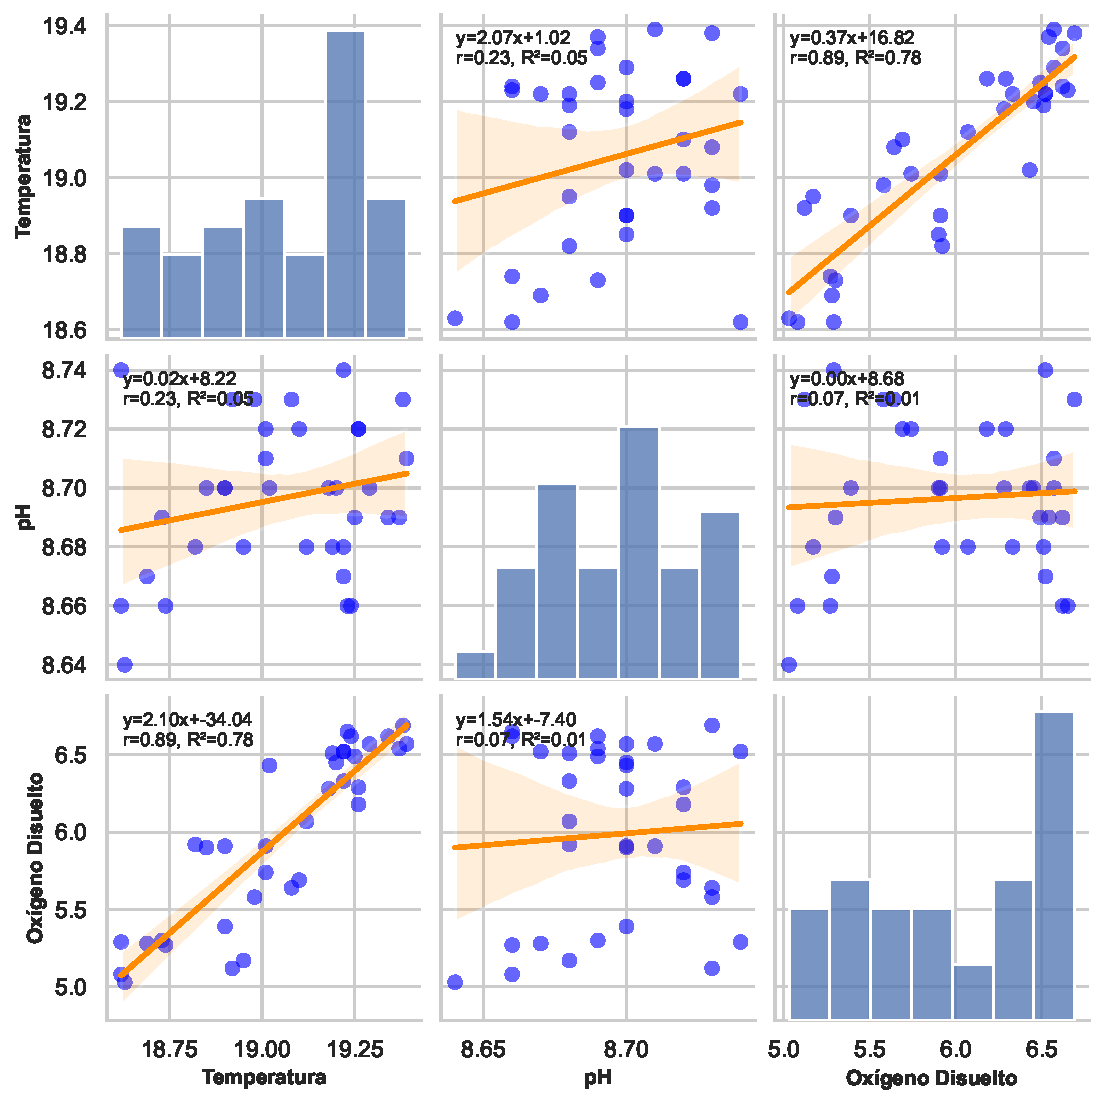
\includegraphics[width=1\linewidth]{Figuras_AED/matriz_de_pares_regresion_colores_fuertes.pdf}
\caption{Matriz de regresión de los parámetros fisicoquímicos en estudio}
\label{fig
}
\end{figure}

\subsubsection{Análisis de la regresión lineal del Oxígeno Disuelto y la Temperatura}

\begin{table}[ht]
\centering
\caption{Análisis estadístico de los residuos para la regresión lineal entre Oxígeno Disuelto y Temperatura}
\label{tab
}
\begin{tabular}{@{}lc@{}}
\toprule
Estadística & Valor \
\midrule
Número de muestras & 35 \
Mediana & 0.02 \
Media & 0.00 \
Desviación Estándar & 0.26 \
Asimetría & -0.41 \
Curtosis & 3.02 \
\bottomrule
\end{tabular}
\end{table}

La Tabla \ref{tab
} presenta las estadísticas de los residuos de la regresión lineal. La Figura \ref{fig
} muestra el histograma y boxplot de estos residuos, indicando una distribución cercana a la normalidad.

\begin{figure}[!htb]
\centering
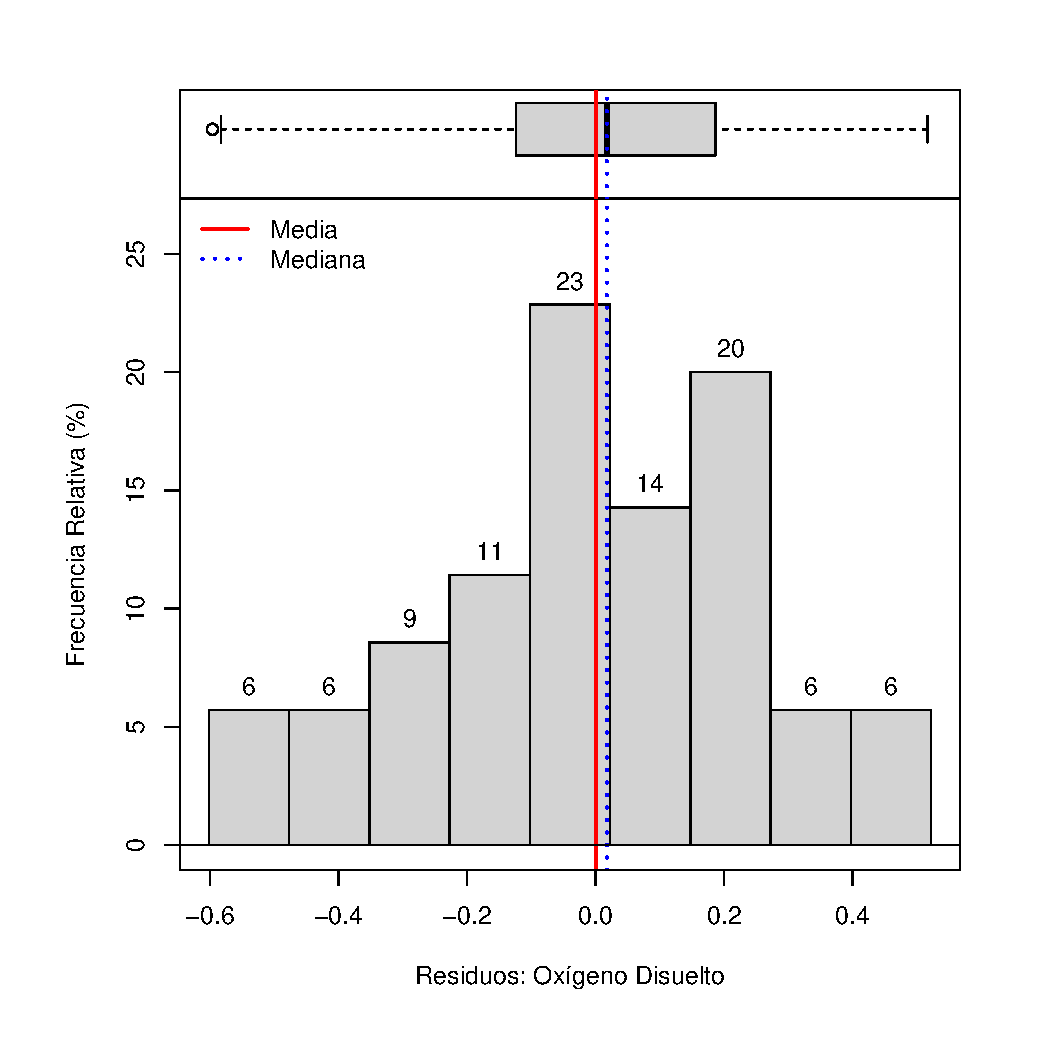
\includegraphics[width=0.5\linewidth]{Figuras_AED/OD_Residual_HistBoxPlot.pdf}
\caption{Histograma y Boxplot de los residuos}
\label{fig
}
\end{figure}

\subsubsection{Ajuste de una distribución normal de los residuos}

La Figura \ref{fig
} presenta cuatro gráficos para evaluar la normalidad de los residuos, que confirman un buen ajuste a la distribución normal.

\begin{figure}[!htb]
\centering
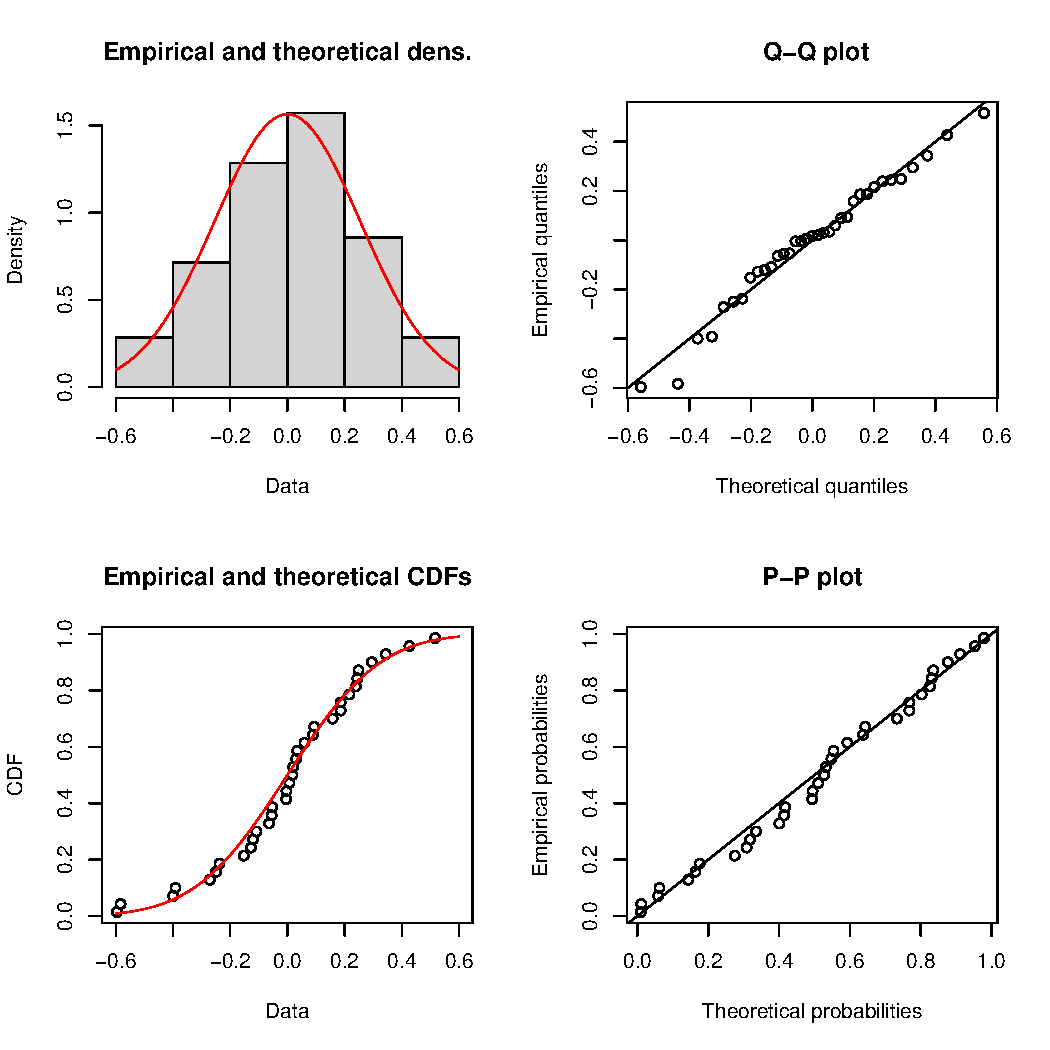
\includegraphics[width=0.9\linewidth]{Figuras_AED/OD_Residual_Fit.pdf}
\caption{Ajuste de una distribución normal de los residuos}
\label{fig
}
\end{figure}

\subsubsection{Pruebas de hipótesis de normalidad}

La Tabla \ref{tab
} muestra que las pruebas de Kolmogorov-Smirnov y Anderson-Darling no rechazan la hipótesis de normalidad de los residuos.

\begin{table}[ht]
\centering
\caption{Resultados de las pruebas de bondad de ajuste para la normalidad}
\label{tab
}
\begin{tabular}{@{}lccc@{}}
\toprule
Método & Nivel de Significancia & P-valor & Decisión \
\midrule
Kolmogorov-Smirnov & 0.05 & 0.92 & No rechazo \
Anderson-Darling & 0.05 & 0.94 & No rechazo \
\bottomrule
\end{tabular}
\end{table}

\subsubsection{Análisis de homocedasticidad y no linealidad}

\begin{table}[H]
\centering
\caption{Resultados de la Prueba de Breusch-Pagan para Homocedasticidad}
\label{tab
}
\begin{tabular}{lc}
\toprule
Estadístico & Valor \
\midrule
Estadístico de Prueba & 0.835 \
Valor-p & 0.361 \
\bottomrule
\end{tabular}
\end{table}

La Prueba de Breusch-Pagan (Tabla \ref{tab
}) no muestra evidencia de heterocedasticidad. La Prueba de Harvey-Collier (Tabla \ref{tab
}) sugiere la presencia de no linealidad en los residuos.

\begin{table}[H]
\centering
\caption{Resultados de la Prueba de Harvey-Collier para No Linealidad}
\label{tab
}
\begin{tabular}{lc}
\toprule
Aspecto & Resultado \
\midrule
Estadístico de Prueba & -2.392 \
Valor-p & 0.023 \
\bottomrule
\end{tabular}
\end{table}
\end{comment}

\section{Análisis exploratorio de datos}

Para esta investigación se analizaron los parámetros Oxígeno Disuelto (mg/L), Temperatura (°C) y pH en la Laguna de Pacucha. Se realizó un estudio estadístico univariado y bivariado para entender las interdependencias dentro del ecosistema acuático.

\subsection{Análisis estadístico univariado}

La Tabla \ref{my-label1} presenta los datos fisicoquímicos obtenidos. Estos datos son fundamentales para elaborar variogramas y analizar la variabilidad espacial de los parámetros.

\begin{table}[!htb]
\centering
\caption{Datos de Temperatura, pH y Oxígeno Disuelto en la Laguna de Pacucha}
\label{my-label1}
\small
\setlength{\tabcolsep}{4pt}
\renewcommand{\arraystretch}{0.9}
\begin{tabular}{@{}cccccc@{}}
\toprule
N° & X & Y & Temperatura (\textdegree{}C) & pH & Oxígeno Disuelto (mg/L) \\ \midrule
1 & 682370.9 & 8493381 & 18.62 & 8.74 & 5.29 \\
2 & 681968.2 & 8493564 & 18.62 & 8.64 & 5.08 \\
3 & 681626.5 & 8493188 & 18.63 & 8.64 & 5.03 \\
4 & 681410.7 & 8493540 & 18.69 & 8.67 & 5.28 \\
5 & 680942.6 & 8493654 & 18.73 & 8.69 & 5.30 \\
6 & 680642.8 & 8493942 & 18.74 & 8.66 & 5.27 \\
7 & 680426.7 & 8494262 & 18.90 & 8.70 & 5.39 \\
8 & 680043.0 & 8494509 & 18.92 & 8.73 & 5.12 \\
9 & 680022.2 & 8494846 & 18.95 & 8.68 & 5.17 \\
10 & 680001.5 & 8495201 & 18.98 & 8.73 & 5.58 \\
11 & 680435.0 & 8495471 & 19.08 & 8.73 & 5.64 \\
12 & 680437.3 & 8495097 & 19.10 & 8.72 & 5.69 \\
13 & 680438.9 & 8494677 & 19.01 & 8.72 & 5.74 \\
14 & 680991.1 & 8494641 & 19.01 & 8.71 & 5.91 \\
15 & 681016.2 & 8494226 & 18.85 & 8.70 & 5.90 \\
16 & 681429.4 & 8494209 & 18.82 & 8.68 & 5.92 \\
17 & 681446.3 & 8494652 & 18.90 & 8.70 & 5.91 \\
18 & 681468.0 & 8495090 & 19.12 & 8.68 & 6.07 \\
19 & 680994.2 & 8495084 & 19.26 & 8.72 & 6.18 \\
20 & 680988.5 & 8495568 & 19.26 & 8.72 & 6.29 \\
21 & 681523.6 & 8495745 & 19.22 & 8.74 & 6.52 \\
22 & 682011.0 & 8495723 & 19.20 & 8.70 & 6.45 \\
23 & 682521.8 & 8495719 & 19.18 & 8.70 & 6.28 \\
24 & 683051.2 & 8495734 & 19.22 & 8.68 & 6.33 \\
25 & 683261.6 & 8495290 & 19.25 & 8.69 & 6.49 \\
26 & 683263.4 & 8494861 & 19.34 & 8.69 & 6.62 \\
27 & 683292.6 & 8494390 & 19.23 & 8.66 & 6.65 \\
28 & 683252.4 & 8493924 & 19.22 & 8.67 & 6.52 \\
29 & 682755.0 & 8493854 & 19.24 & 8.66 & 6.62 \\
30 & 682478.8 & 8494211 & 19.19 & 8.68 & 6.51 \\
31 & 682486.6 & 8494677 & 19.37 & 8.69 & 6.54 \\
32 & 682517.5 & 8495110 & 19.29 & 8.70 & 6.57 \\
33 & 681992.6 & 8495105 & 19.39 & 8.71 & 6.57 \\
34 & 681957.2 & 8494676 & 19.38 & 8.73 & 6.69 \\
35 & 681954.0 & 8494210 & 19.02 & 8.70 & 6.43 \\ \bottomrule
\end{tabular}
\end{table}

\subsubsection{Estadísticos Básicos de los parámetros}

La Tabla \ref{tab:combined_statistics} muestra estadísticas descriptivas de los parámetros medidos.

\begin{table}[!htb]
\centering
\caption{Estadísticos descriptivos para Temperatura, Oxígeno Disuelto y pH}
\label{tab:combined_statistics}
\begin{tabular}{lccc}
\toprule
 & Temperatura & Oxígeno Disuelto & pH  \\
\midrule
n & 35 & 35 & 35 \\
Mínimo & 18.62 & 5.03 & 8.64 \\
Mediana & 19.10 & 6.07 & 8.70 \\
Media & 19.06 & 5.99 & 8.70 \\
Máximo & 19.39 & 6.69 & 8.74 \\
Desviación Estándar & 0.23 & 0.56 & 0.03 \\
Asimetría & -0.45 & -0.35 & -0.25 \\
Curtosis & 2.04 & 1.64 & 2.39 \\
\bottomrule
\end{tabular}
\end{table}

\subsubsection{Histogramas y Boxplot}

\begin{figure}[!htb]
    \centering
    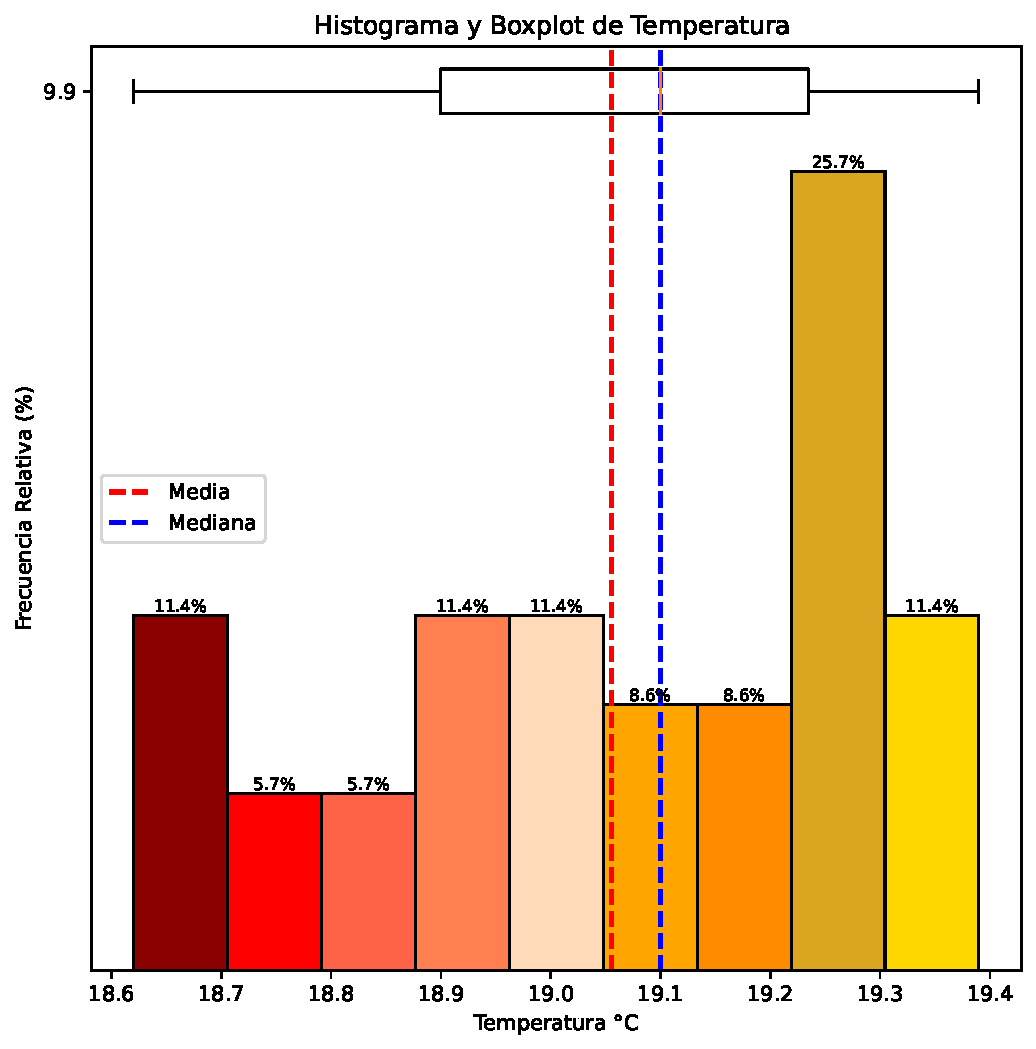
\includegraphics[width=0.5\linewidth]{Figuras_AED/Histograma_Temperatura.pdf}
    \caption{Frecuencia y Rango de la Temperatura}
    \label{fig:enter-label1}
\end{figure}

La Figura \ref{fig:enter-label1} muestra el histograma y boxplot de las temperaturas. La mayoría de las temperaturas se concentran entre 19.2 y 19.3 °C. 

\begin{figure}[!htb]
    \centering
    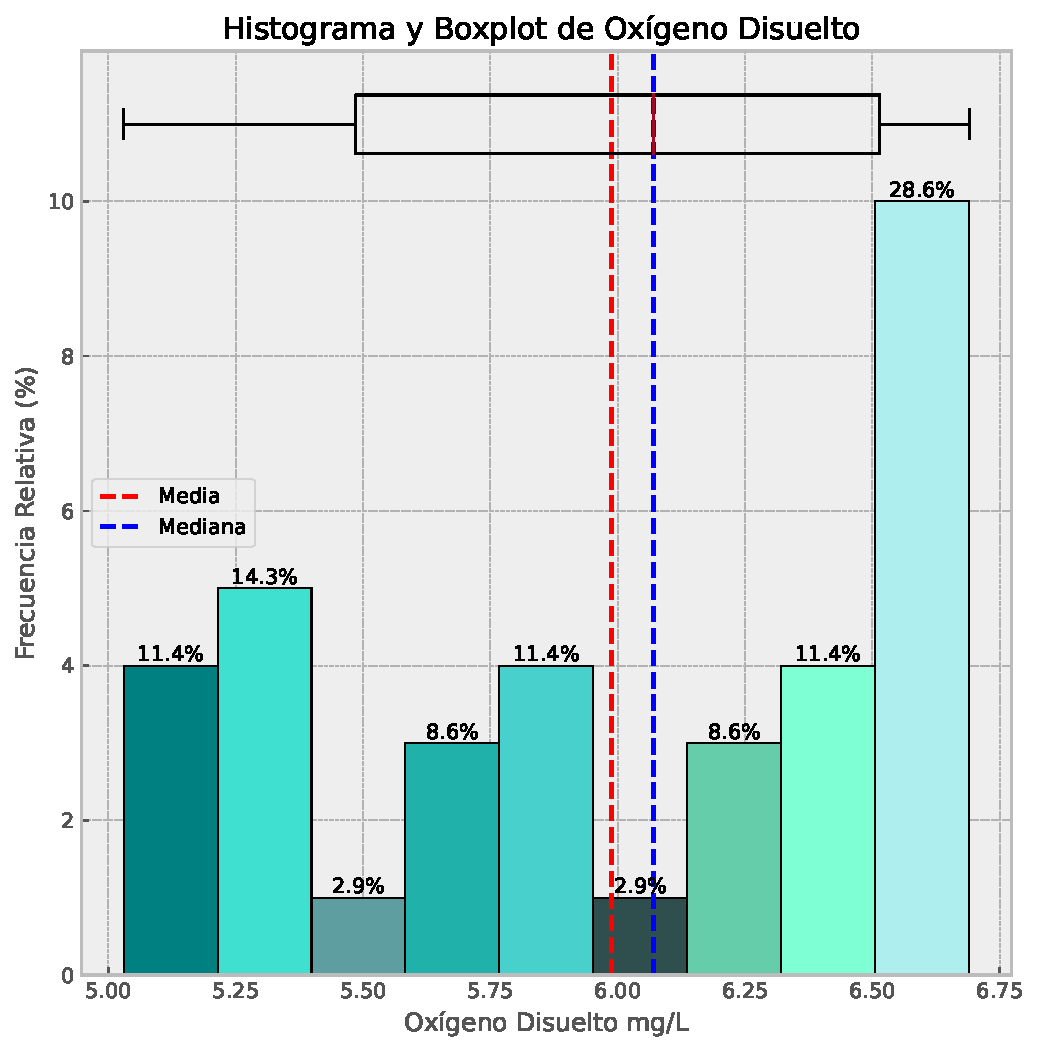
\includegraphics[width=0.5\linewidth]{Figuras_AED/Histograma_Oxigeno_Disuelto.pdf}
    \caption{Frecuencia y Rango del Oxígeno Disuelto}
    \label{fig:enter-label2}
\end{figure}

La Figura \ref{fig:enter-label2} ilustra las concentraciones de oxígeno disuelto, siendo 6.5-6.7 mg/L el rango más común.

\begin{figure}[!htb]
    \centering
    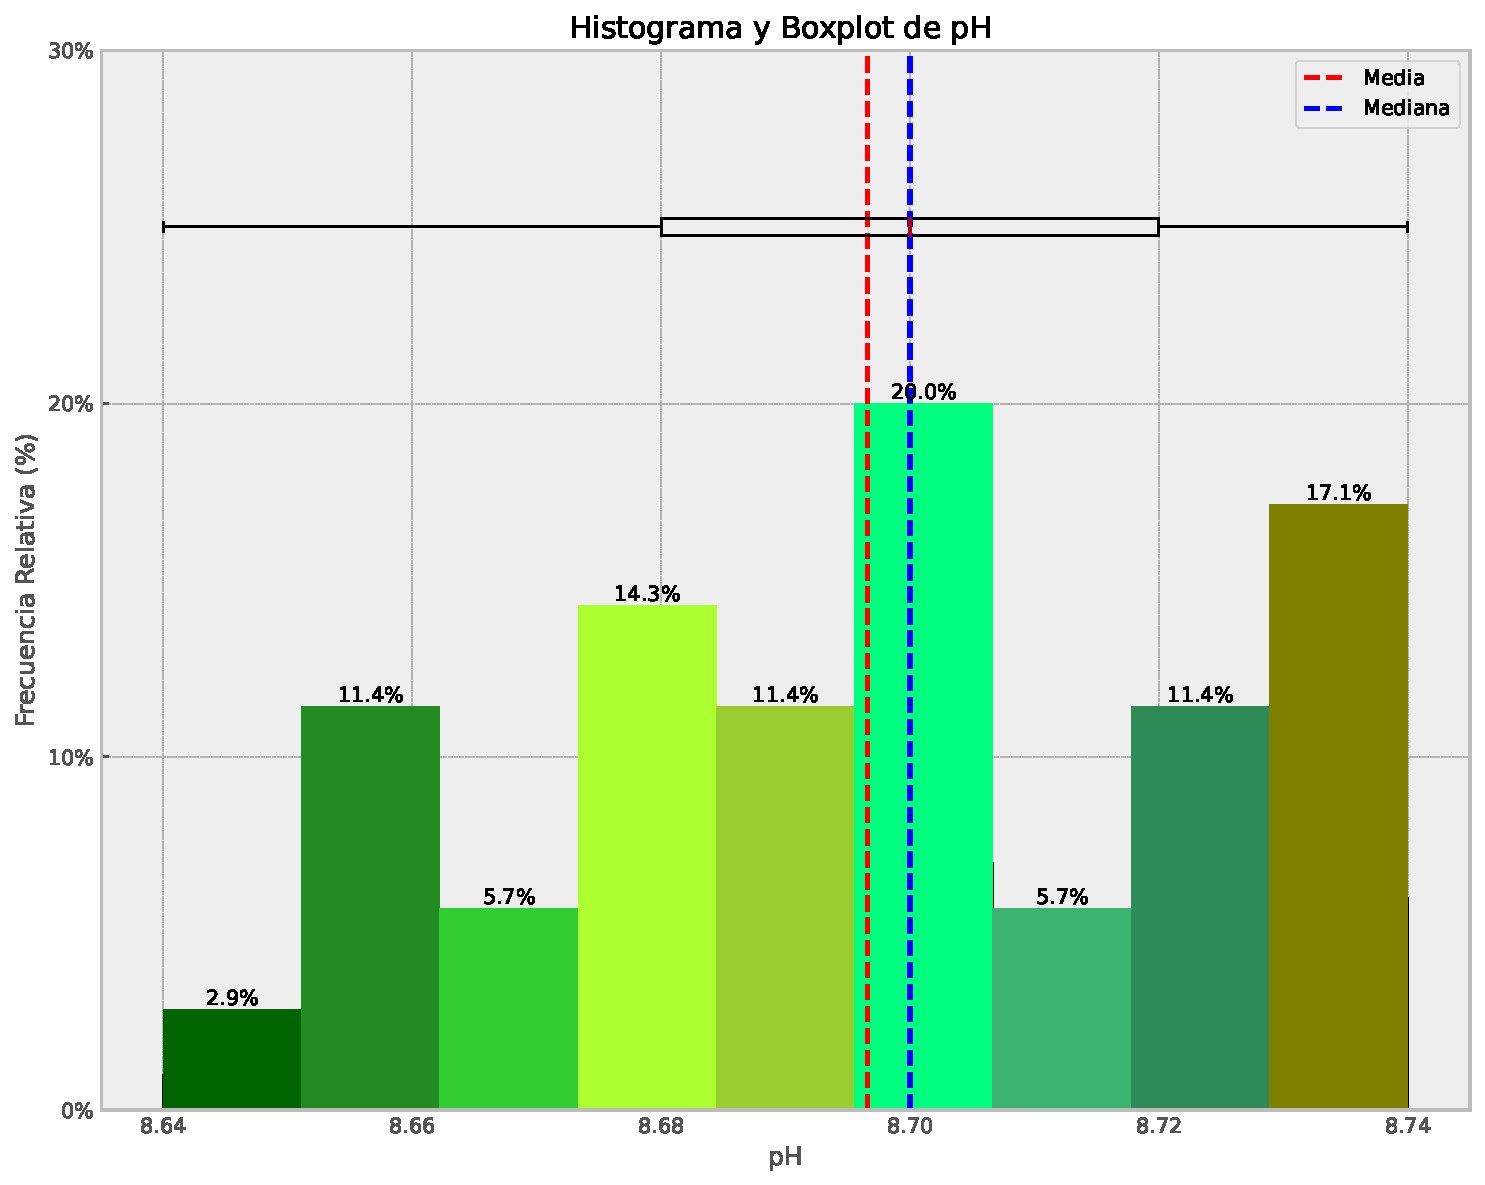
\includegraphics[width=0.5\linewidth]{Figuras_AED/Histograma_pH.pdf}
    \caption{Frecuencia y Rango del pH}
    \label{fig:enter-label4}
\end{figure}

La Figura \ref{fig:enter-label4} representa los valores de pH, concentrados alrededor de 8.70.

\subsection{Análisis estadístico bivariado}
 \subsubsection{Análisis de correlación }

 La Tabla \ref{tab:correlation} presenta los coeficientes de correlación entre los parámetros fisicoquímicos Oxígeno Disuelto (OD), Temperatura y pH en la Laguna de Pacucha, utilizando los métodos de Pearson, Spearman y Kendall. Los resultados indican que la correlación más fuerte se encuentra entre la Temperatura y el Oxígeno Disuelto, con coeficientes de \(r = 0.89\) (Pearson), \(\rho = 0.88\) (Spearman) y \(\tau = 0.70\) (Kendall). Esta fuerte relación sugiere que este par de variables es adecuado para la elaboración de un covariograma y para el cokriging, ya que la alta correlación indica una dependencia significativa que puede ser modelada conjuntamente. En contraste, las correlaciones entre Oxígeno Disuelto y pH, así como entre Temperatura y pH, son mucho más débiles, lo que las hace menos adecuadas para estos análisis geoestadísticos.

\begin{table}[!htb]
\centering 
\caption{Coeficientes de correlación entre las variables fisicoquímicas}
\label{tab:correlation}
\begin{tabular}{@{}lccc@{}}
\toprule
Método & OD y pH & Temperatura y pH & OD y Temperatura \\ \midrule
Pearson & 0.07 & 0.23 & 0.89 \\
Spearman & 0.02 & 0.17 & 0.88 \\
Kendall & -0.02 & 0.12 & 0.70 \\ \bottomrule
\end{tabular}
\end{table}

\subsubsection{Regresión Lineal}


La Figura \ref{fig:enter-matriz_regre} ilustra una matriz de regresión que incorpora histogramas y gráficos de dispersión con líneas de regresión para las combinaciones de los parámetros fisicoquímicos: Temperatura, pH y Oxígeno Disuelto. A continuación se detallan las observaciones más significativas:

\textbf{Temperatura vs. Oxígeno Disuelto:} Se observa una correlación positiva sustancial entre estos dos parámetros, con un coeficiente de correlación de \( r = 0.89 \) y un coeficiente de determinación de \( R^2 = 0.78 \). La ecuación de la regresión lineal es \( y = 0.37x + 16.82 \), indicando que incrementos en la temperatura están fuertemente asociados con aumentos en los niveles de oxígeno disuelto. Este hallazgo sugiere una interdependencia significativa que puede ser crítica para modelar y predecir la calidad del agua en este entorno.
\textbf{Temperatura vs. pH}: La relación entre la Temperatura y el pH es considerablemente más débil, con un coeficiente de correlación de \( r = 0.23 \) y un \( R^2 = 0.05 \). La ecuación de la regresión lineal, \( y = 0.02x + 8.22 \), refleja que la temperatura no es un predictor eficaz del pH. Esto implica que otros factores podrían tener una mayor influencia sobre el pH en la Laguna de Pacucha.

\textbf{pH vs. Oxígeno Disuelto:} La correlación entre el pH y el Oxígeno Disuelto es prácticamente inexistente, con un coeficiente de correlación de \( r = 0.07 \) y un \( R^2 = 0.01 \). La ecuación de la regresión lineal, \( y = 0.00x + 8.68 \), confirma la ausencia de una relación significativa entre estas dos variables.
- **Histogramas:** Los histogramas situados en la diagonal de la matriz proporcionan una visión general de la distribución de cada parámetro. La Temperatura y el pH muestran distribuciones relativamente uniformes, mientras que el Oxígeno Disuelto presenta una ligera concentración alrededor de ciertos valores, indicando una variabilidad moderada.

Estas correlaciones y distribuciones subrayan la importancia de la Temperatura y el Oxígeno Disuelto como variables interrelacionadas en el ecosistema de la Laguna de Pacucha, mientras que el pH parece comportarse de manera más independiente. Estos hallazgos son esenciales para la elaboración de modelos geoestadísticos y estrategias de gestión ambiental.



\begin{figure}[!htb]
    \centering
    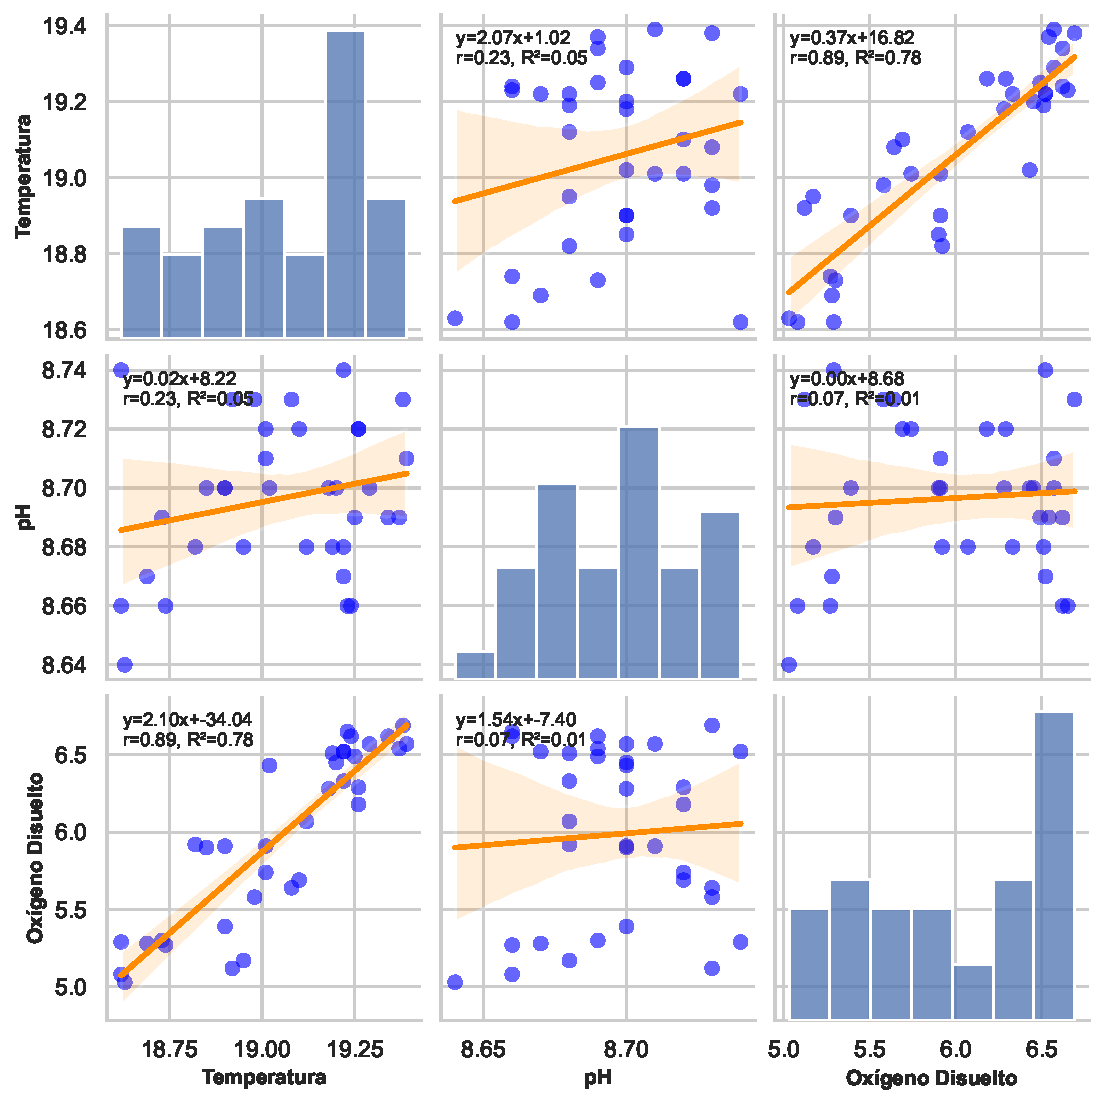
\includegraphics[width=1\linewidth]{Figuras_AED/matriz_de_pares_regresion_colores_fuertes.pdf}
    \caption{Matriz de regresión de los parámetros fisicoquímicos en estudio}
    \label{fig:enter-matriz_regre}
\end{figure}

\subsection{Análisis de la regresión lineal del Oxígeno Disuelto y la Temperatura}


\subsubsection{Análisis de los residuos de la Regresión lineal Oxígeno Disuelto y  Temperatura}
\begin{table}[ht]
\centering
\caption{Análisis estadístico de los residuos para la regresión lineal entre Oxígeno Disuelto y Temperatura}
\label{tab:residual_statistics}
\begin{tabular}{@{}lc@{}}
\toprule
\textbf{Estadística} & \textbf{ } \\
\midrule
Número de muestras & 35 \\
Mediana & 0.02 \\
Media & 0.00 \\
Desviación Estándar & 0.26 \\
Asimetría & -0.41 \\
Curtosis & 3.02 \\
\bottomrule
\end{tabular}
\end{table}

La Tabla \ref{tab:residual_statistics} presenta las estadísticas de los residuos de la regresión lineal. La Figura \ref{fig:enter-labelod} muestra el histograma y boxplot de estos residuos, indicando una distribución cercana a la normalidad.

\begin{figure}[!htb]
    \centering
    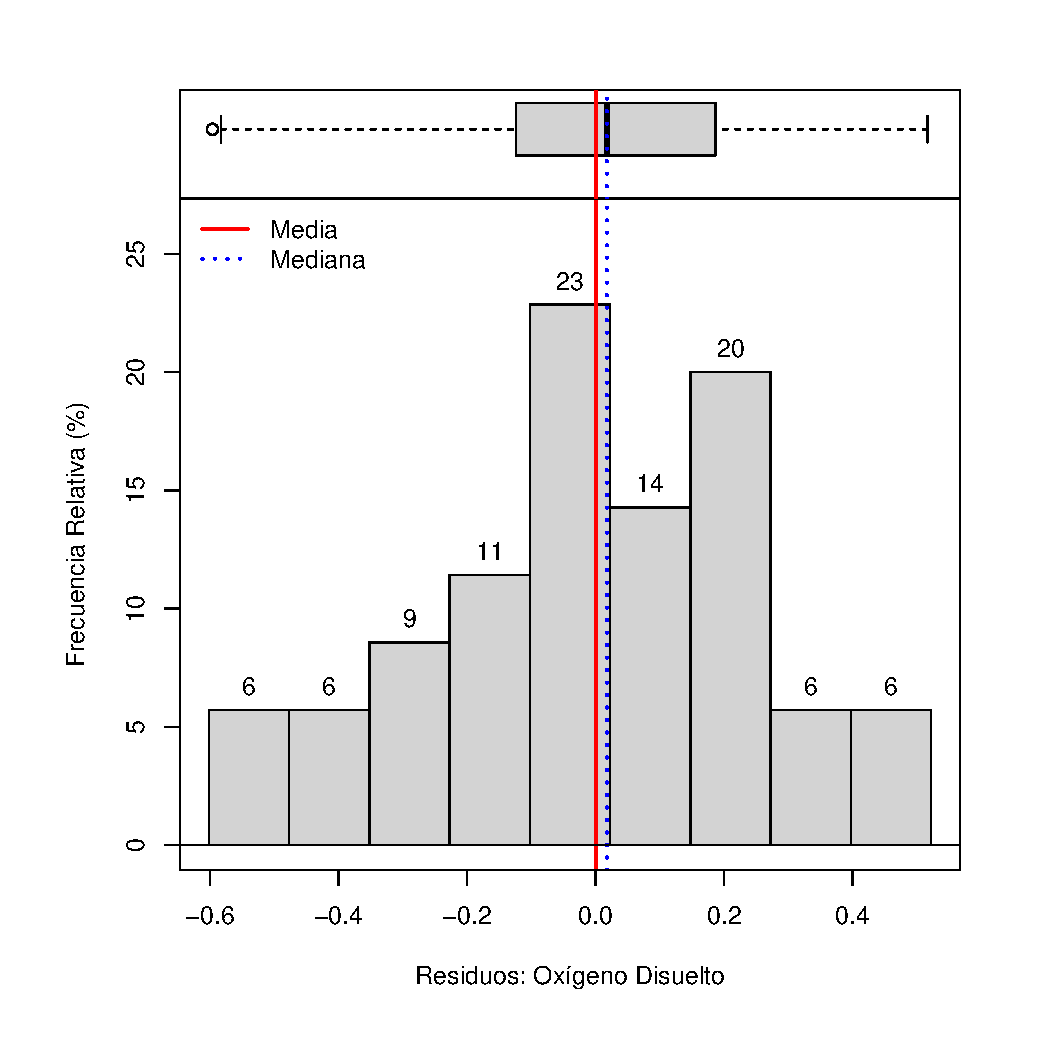
\includegraphics[width=0.5\linewidth]{Figuras_AED/OD_Residual_HistBoxPlot.pdf}
    \caption{Histograma y Boxplot de los residuos}
    \label{fig:enter-labelod}
\end{figure}

\begin{comment}
    


\subsubsection{Ajuste de una distribución normal de los residuos}

La Figura \ref{fig:enter-labelRES} presenta cuatro gráficos para evaluar la normalidad de los residuos, que confirman un buen ajuste a la distribución normal.

\begin{figure}[!htb]
    \centering
    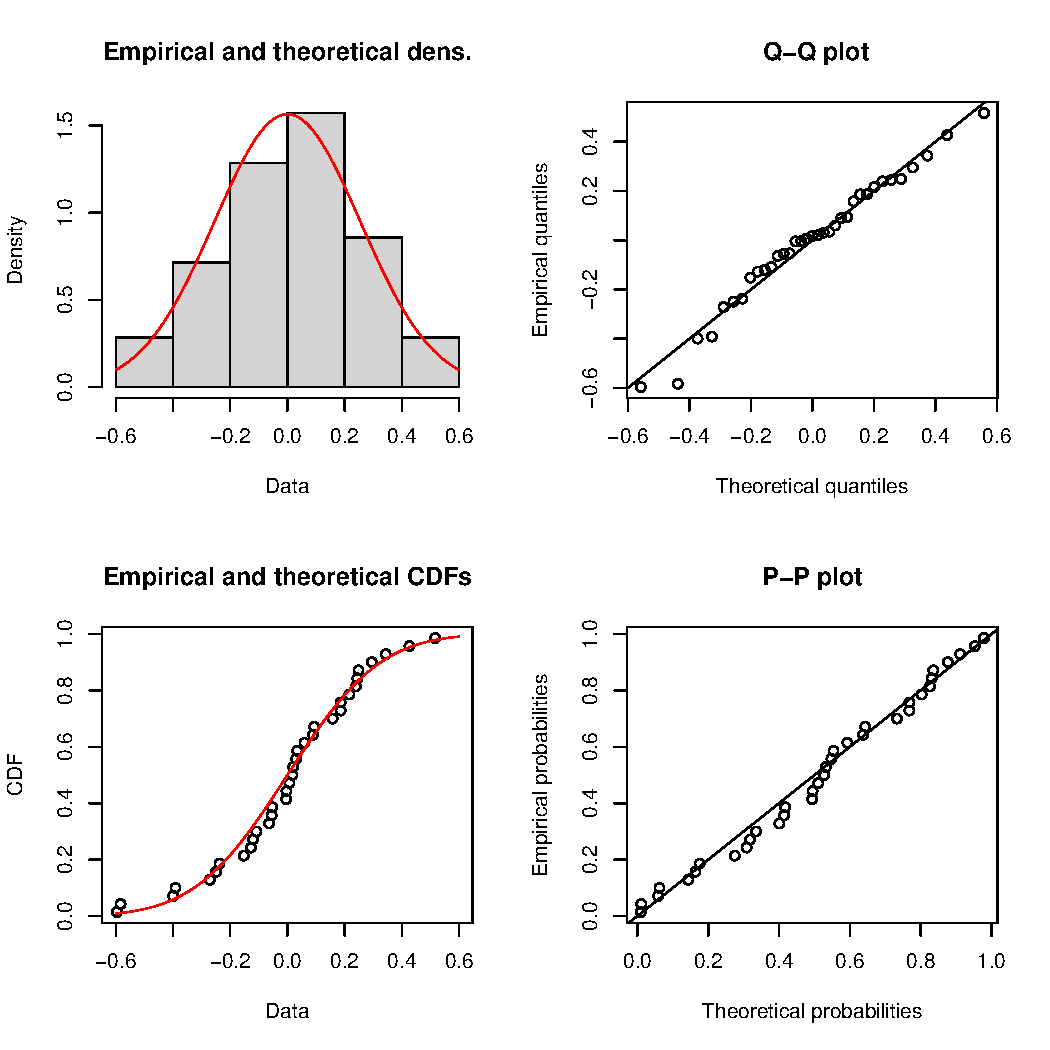
\includegraphics[width=0.9\linewidth]{Figuras_AED/OD_Residual_Fit.pdf}
    \caption{Ajuste de una distribución normal de los residuos}
    \label{fig:enter-labelRES}
\end{figure}

\end{comment}

\subsubsection{Pruebas de hipótesis de normalidad}

La Tabla \ref{tab:goodness_of_fit_tests} muestra que las pruebas de Kolmogorov-Smirnov y Anderson-Darling no rechazan la hipótesis de normalidad de los residuos.

\begin{table}[ht]
\centering
\caption{Resultados de las pruebas de bondad de ajuste para la normalidad}
\label{tab:goodness_of_fit_tests}
\begin{tabular}{@{}lccc@{}}
\toprule
Método & Nivel de Significancia & P-valor & Decisión \\
\midrule
Kolmogorov-Smirnov & 0.05 & 0.92 & No rechazo \\
Anderson-Darling & 0.05 & 0.94 & No rechazo \\
\bottomrule
\end{tabular}
\end{table}

\subsubsection{Análisis de homocedasticidad y no linealidad}

\begin{table}[H]
\centering
\caption{Resultados de la Prueba de Breusch-Pagan para Homocedasticidad}
\label{tab:breusch_pagan_test}
\begin{tabular}{lc}
\toprule
Estadístico & Valor \\
\midrule
Estadístico de Prueba & 0.835 \\
Valor-p & 0.361 \\
\bottomrule
\end{tabular}
\end{table}

La Prueba de Breusch-Pagan (Tabla \ref{tab:breusch_pagan_test}) no muestra evidencia de heterocedasticidad. La Prueba de Harvey-Collier (Tabla \ref{tab:harvey_collier_test}) sugiere la presencia de no linealidad en los residuos.

\begin{table}[H]
\centering
\caption{Resultados de la Prueba de Harvey-Collier para No Linealidad}
\label{tab:harvey_collier_test}
\begin{tabular}{lc}
\toprule
Aspecto & Resultado \\
\midrule
Estadístico de Prueba & -2.392 \\
Valor-p & 0.023 \\
\bottomrule
\end{tabular}
\end{table}
 

\section{Análisis Variográfico}

El objetivo de este análisis es entender la estructura espacial y la correlación de las variables ambientales medidas, como la temperatura, el oxígeno disuelto y el pH. Se utiliza la técnica del variograma para ilustrar cómo la variabilidad espacial de estas variables se modifica en función de la distancia.


\subsection{Temperatura}
\subsubsection{Distribución espacial de la Temperatura}

La Figura \ref{fig:enter-labeld} muestra la distribución espacial de la temperatura en la Laguna de Pacucha mediante un diagrama de dispersión, con las coordenadas geográficas de 35 ubicaciones trazadas en los ejes X e Y. Los colores varían del azul al rojo, indicando temperaturas de bajas a altas, permitiendo una identificación clara de las zonas térmicas. La leyenda clasifica las temperaturas en nueve intervalos, con barras de frecuencia que indican el número de observaciones por rango. Un histograma en la esquina inferior derecha presenta la distribución de frecuencias de las temperaturas, destacando los rangos predominantes. Estas visualizaciones proporcionan una comprensión clara de la variabilidad térmica y las posibles relaciones espaciales en el ecosistema acuático.
\begin{figure} [H]
    \centering
    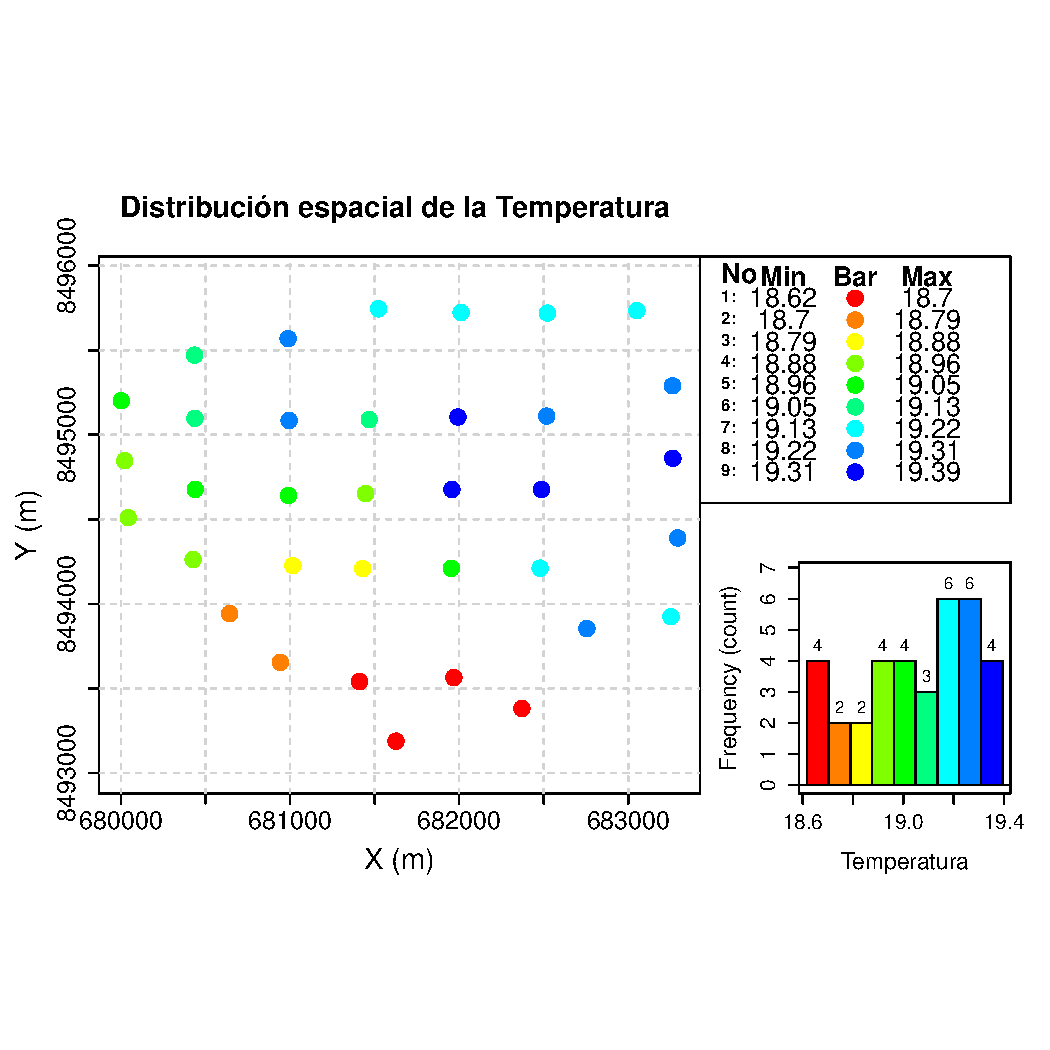
\includegraphics[width=0.8\linewidth]{Figuras_AED//VARIOGRAFICO/tem_Spatial_Distr.pdf}
    \caption{Distribución espacial de la Temperatura (° C) en la laguna de Pacucha}
    \label{fig:enter-labeld}
\end{figure}




\begin{comment}
    
\subsubsection{Análisis de tendencias de la temperatura }

\begin{figure} [!htb]
    \centering
    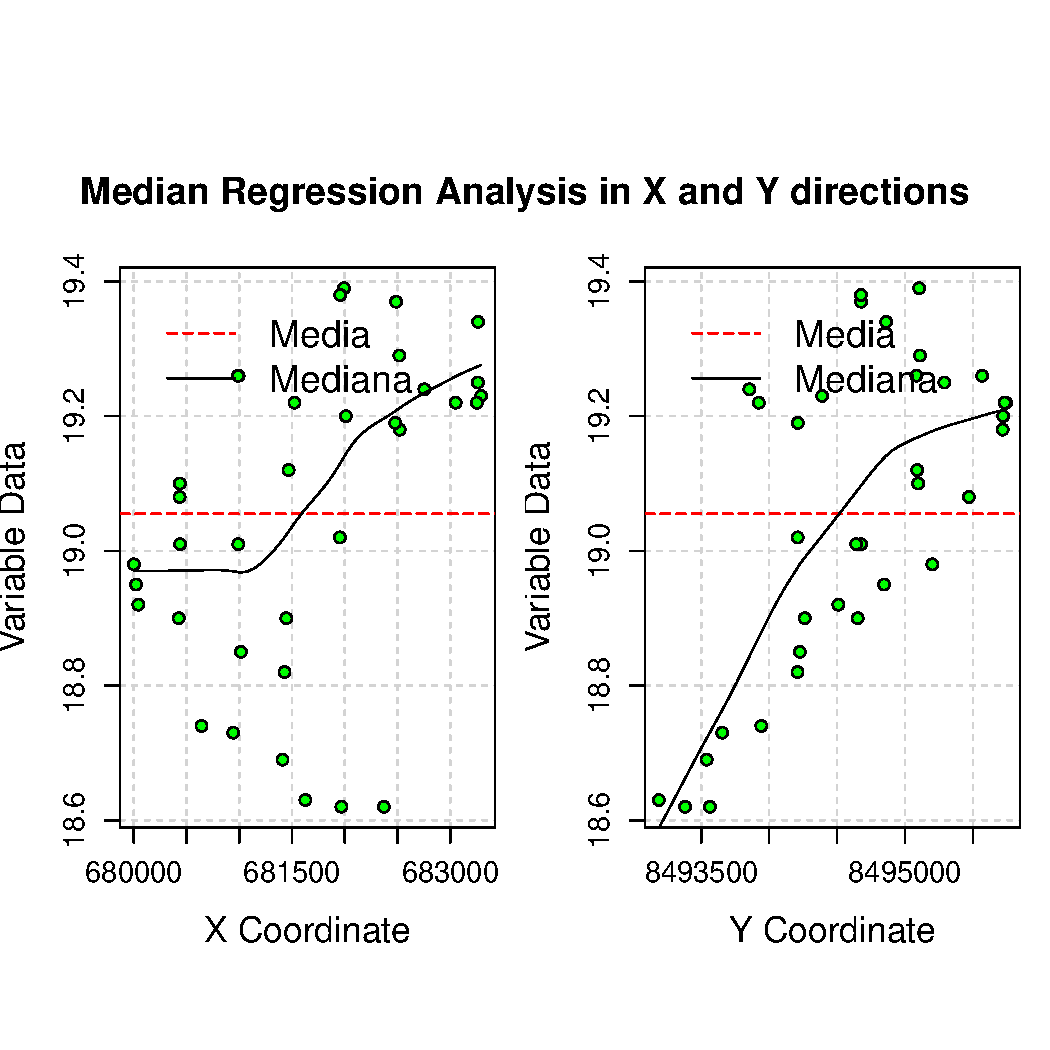
\includegraphics[width=0.7\linewidth]{Figuras_AED//VARIOGRAFICO/tem_Trend_X_Y.pdf}
    \caption{Análisis de regresión de la mediana en las direcciones X e Y para la variable Temperatura}
    \label{fig:enter-label23}
\end{figure}
La Figura \ref{fig:enter-label23}  muestra dos gráficos de dispersión que representan el análisis de regresión de la mediana para una variable de interés en relación con las coordenadas X e Y. En el gráfico de la izquierda, correspondiente al eje X, se puede observar una ligera tendencia ascendente en la mediana, lo que sugiere que la variable podría aumentar con la longitud. La dispersión de los puntos alrededor de la línea de mediana indica una posible variabilidad en los datos. Por otro lado, el gráfico de la derecha, correspondiente al eje Y, muestra una dispersión de puntos que sugiere variabilidad en la variable con la latitud, aunque los puntos están más concentrados hacia el extremo superior. La línea de mediana, que representa la tendencia central, indica una relación potencial entre la variable y la dirección Y. Aunque estos patrones visuales proporcionan una indicación inicial de estacionariedad, la falta de uniformidad en la dispersión de los puntos alrededor de las medianas y las tendencias observadas podrían sugerir la presencia de no estacionariedad en los datos, lo que requeriría análisis estadísticos adicionales para confirmar.

\end{comment}


\subsubsection{Modelización univariante de la variografía Temperatura }
\begin{enumerate}
    \item \subsubsection{Variogramas direccionales (0, 45, 90 y 135)}


\begin{figure}[H]
    \centering
    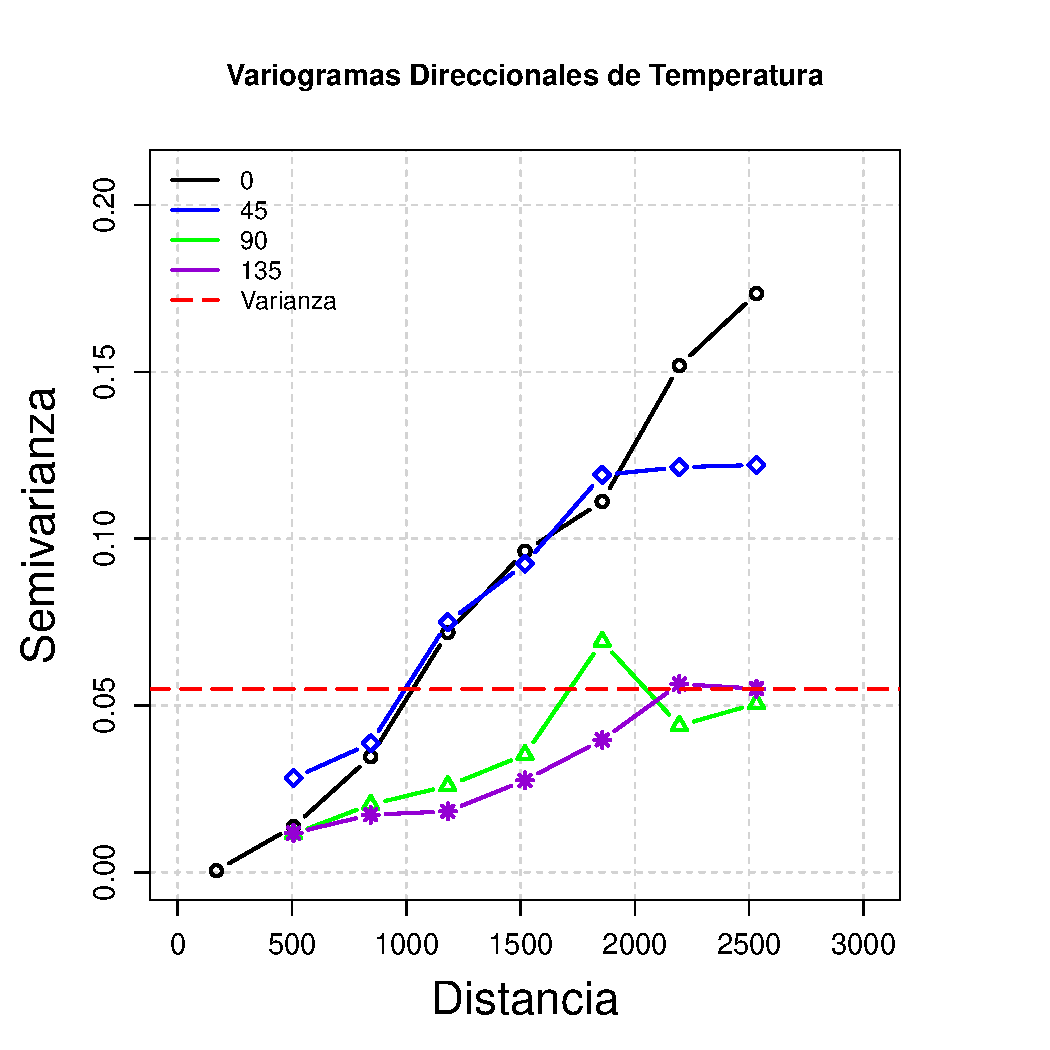
\includegraphics[width=0.8\linewidth]{Figuras_AED//VARIOGRAFICO/tem_Vario4DEstimation.pdf}
    \caption{Análisis comparativo de variogramas direccionales para la temperatura}

    \label{fig:enter-labelter}
\end{figure}

La Figura \ref{fig:enter-labelter} de los variogramas direccionales para la temperatura revela información crítica sobre la estructura espacial y la anisotropía del campo térmico. El variograma direccional a 0° muestra un aumento constante en la semivarianza con la distancia, sugiriendo una fuerte anisotropía en la dirección norte-sur. En contraste, el variograma a 45° alcanza su meseta más rápidamente, indicando que la correlación entre las mediciones disminuye más lentamente y se estabiliza a una distancia más corta. Las direcciones de 90° y 135° presentan patrones erráticos, sugiriendo variaciones térmicas locales y estructuras complejas. Es crucial destacar que todos los variogramas se acotan en la meseta y ninguno excede la varianza global, lo que sugiere que la hipótesis de estacionariedad es válida. Este análisis es esencial para la modelización geoestadística y la implementación de técnicas de interpolación, como el Kriging anisotrópico, optimizando la predicción de temperaturas en ubicaciones no medidas.


 \item \subsubsection{Ajuste automático del modelo de variograma para la temperatura}

\begin{figure}[H]
    \centering
    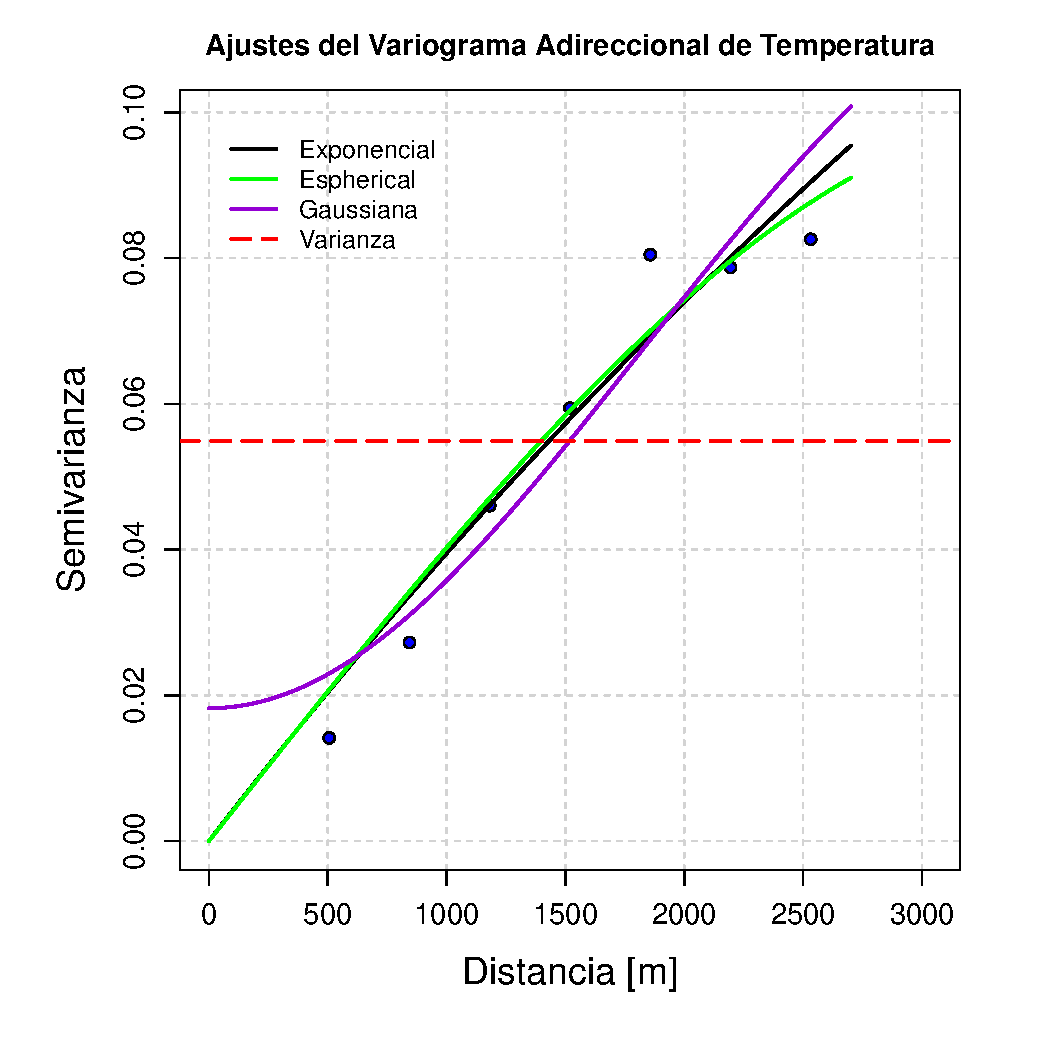
\includegraphics[width=0.8\linewidth]{Figuras_AED//VARIOGRAFICO/tem_VarioAllModelEstimation.pdf}
    \caption{Ajustes de los variogramas modelos para la temperatura}
    \label{fig:enter-labelmodel}
\end{figure}

 Al observar la Figura \ref{fig:enter-labelmodel}, se puede apreciar que los modelos exponencial y esférico ajustan bien los datos a distancias cortas, pero divergen en distancias mayores. En contraste, el modelo gaussiano muestra un ajuste preciso en todas las distancias, siguiendo de cerca los puntos experimentales y manteniéndose dentro de la varianza global sin sobrepasarla. Esto sugiere que el modelo gaussiano es el más adecuado para modelar la semivarianza de la temperatura en este caso, ya que capta la continuidad espacial de los datos de manera eficaz. Sin embargo, la selección final del modelo debe incluir una validación cruzada y considerar el contexto de la zona de estudio, como gradientes térmicos o estructuras geológicas. La elección del modelo óptimo permitirá predicciones más precisas en la interpolación geoestadística y mejorará la comprensión del comportamiento térmico en la Laguna de Pacucha.

\begin{comment}
    
 \item \subsubsection{Mejor ajuste automático del modelo de variograma para la temperatura}

\begin{figure}[!htb]
    \centering
    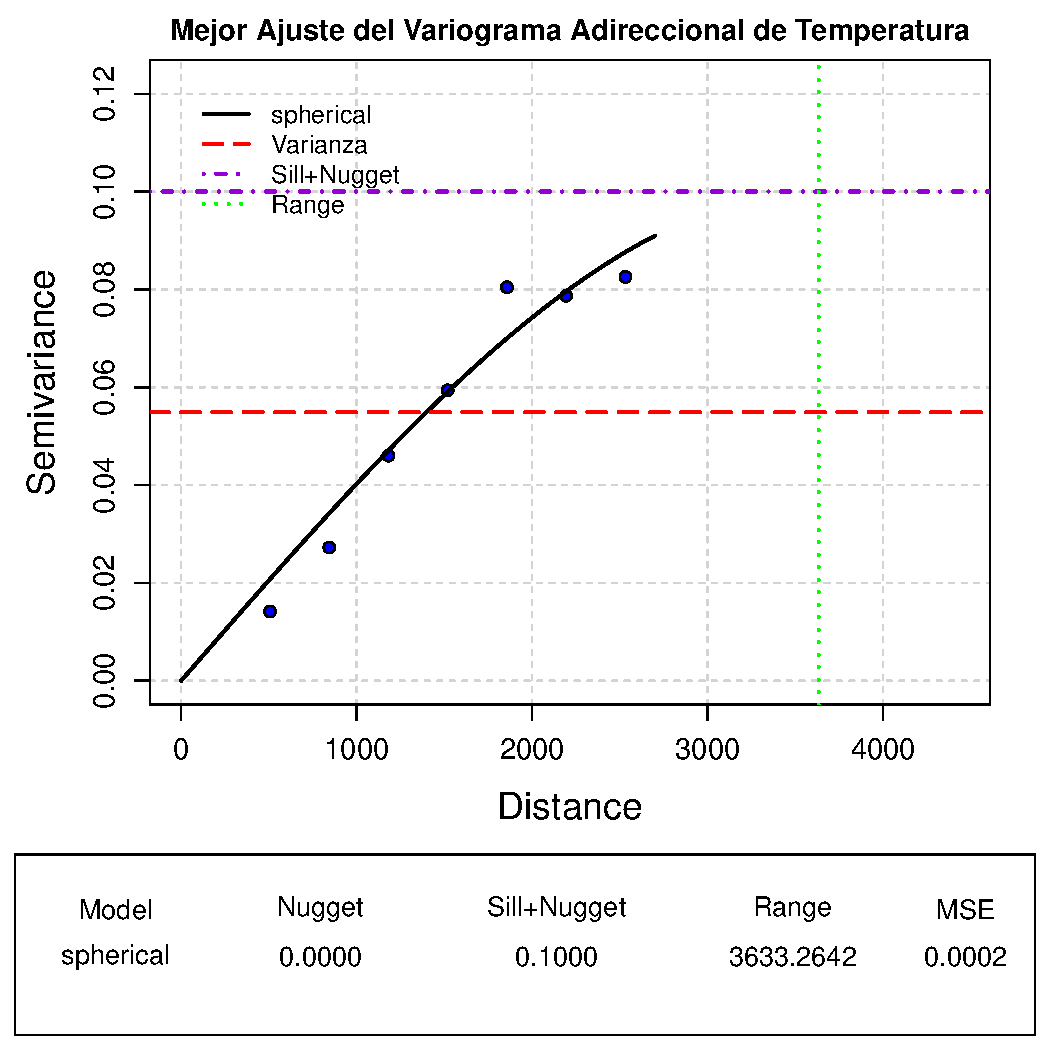
\includegraphics[width=0.7\linewidth]{Figuras_AED//VARIOGRAFICO/teme_VarioBestModelEstimation.pdf}
    \caption{Mejor modelo de variograma ajustado para la temperatura}
    \label{fig:enter-labelzx1}
\end{figure}

La Figura \ref{fig:enter-labelzx1} muestra un variograma etiquetado "Mejor ajuste del variograma direccional azimutal de temperatura", indicando que el gráfico representa el modelo que mejor se ajusta a los datos de temperatura en una dirección específica. El gráfico lineal representa el modelo esférico, como indica la leyenda, y se ajusta a los puntos de datos marcados en el gráfico. Estos puntos de datos circulares azules se distribuyen a lo largo del eje X, que representa la distancia en metros, mientras que el eje Y muestra la semivarianza de los datos de temperatura.

El modelo esférico no muestra un efecto pepita, como demuestra el valor de 0,0000 en la tabla de parámetros situada debajo del gráfico, lo que sugiere que no hay variabilidad no detectada a distancias muy cortas. El "umbral", que es el valor en el que se estabiliza el variograma, se combina con el efecto nugget y da un valor de 0,1000, que parece ser coherente con la varianza global indicada por la línea roja horizontal discontinua del gráfico. El intervalo, representado por la línea verde punteada vertical, es donde el modelo alcanza el umbral, situado aproximadamente a 3633,2642 metros, lo que indica la distancia más allá de la cual los puntos dejan de estar correlacionados.


 Una posible crítica a esta visualización podría señalar que el modelo esférico proporciona un ajuste razonable a los datos, como sugiere el bajo error cuadrático medio (RMSE) de 0,0002, lo que indica una alta precisión del modelo a la hora de representar la variabilidad espacial de los datos de temperatura. Sin embargo, para un análisis más exhaustivo, sería beneficioso comparar este ajuste con otros modelos geoestadísticos para validar que el modelo esférico es realmente el más apropiado. Además, aunque el modelo esférico se ajusta bien a los datos, hay que ser prudente a la hora de interpretar los resultados, asegurándose de que el modelo y sus parámetros son coherentes con el conocimiento físico y geológico de la zona de estudio.
\end{comment}

 \item \subsubsection{Ajuste manual del modelo de variograma para la temperatura}

 \begin{figure}[!htb]
     \centering
     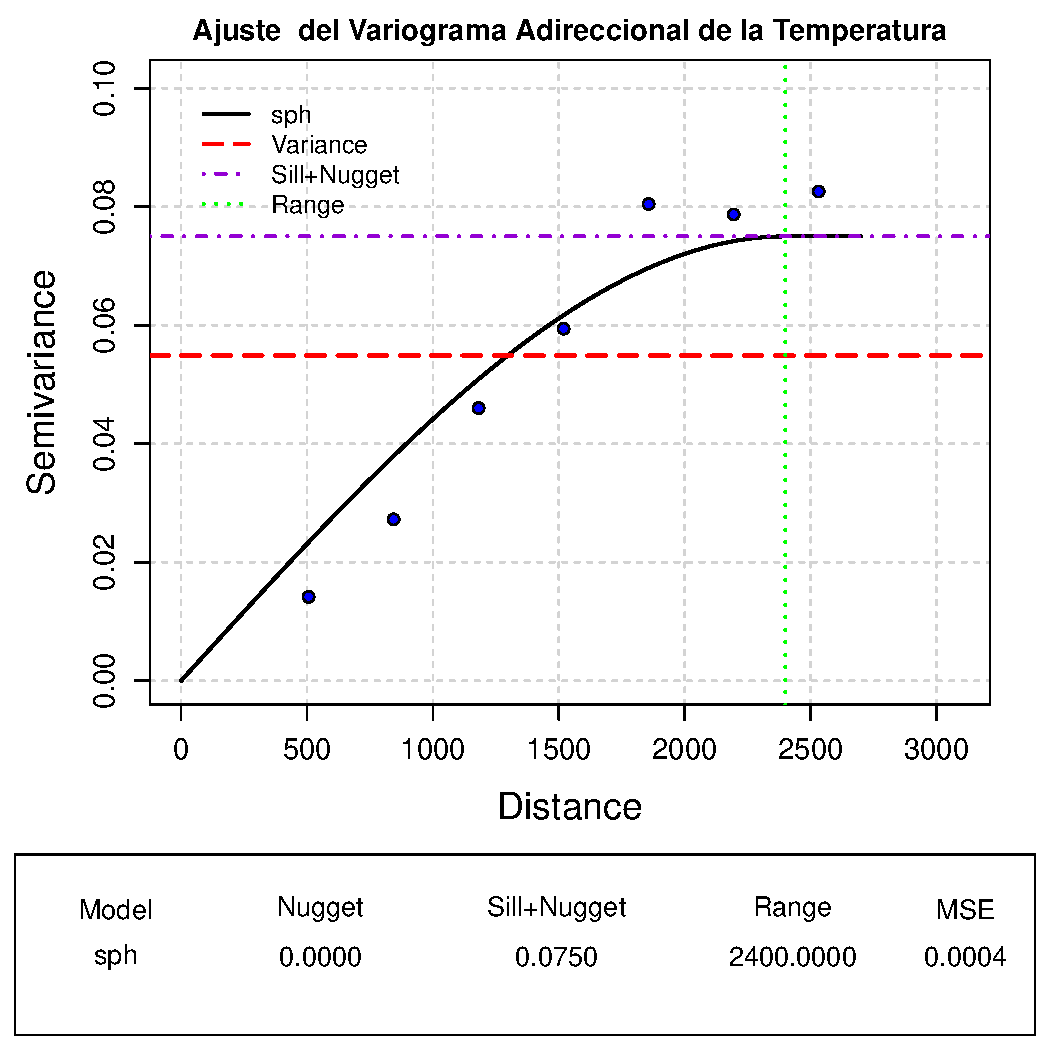
\includegraphics[width=0.8\linewidth]{Figuras_AED//VARIOGRAFICO/temperatura_VarioEyeEstimation.pdf}
     \caption{Optimización Manual del Modelo Esférico del Variograma  Temperatura}

     \label{fig:enter-labelaq}
 \end{figure}

  La Figura \ref{fig:enter-labelaq} ilustra el ajuste manual de un modelo esférico al variograma de datos de temperatura, utilizado para analizar la variabilidad espacial. Los círculos azules muestran la semivarianza a distintas distancias, y la línea negra continua representa el modelo esférico ajustado. El valor Nugget de 0,0000 indica la ausencia de variabilidad a pequeña escala o errores no considerados, mientras que el \textit{Sill+Nugget} de 0,0750 se alinea con la varianza total mostrada por la línea roja. La línea verde vertical a 2.400 metros marca el Rango, donde las observaciones se vuelven independientes. El error cuadrático medio (ECM) de 0,0004 sugiere un ajuste preciso del modelo, lo que es clave para aplicaciones futuras como la interpolación de datos mediante kriging.


 \end{enumerate}

\subsubsection{ Validación cruzada del modelo de variograma esférico para la temperatura}

\begin{longtable}{cccccc} 

\caption{Validación cruzada del modelo esférico para la temperatura} \label{tab:cross_validation} \\
\hline
\textbf{ID} & \textbf{X} & \textbf{Y} & \textbf{Z} & \textbf{Z*} & \textbf{Z-Z*} \\
\hline
\endfirsthead
\multicolumn{6}{c}%
{\tablename\ \thetable\ -- \textit{Continuación de la página anterior}} \\
\hline
\textbf{ID} & \textbf{X} & \textbf{Y} & \textbf{Z} & \textbf{Z*} & \textbf{Z-Z*} \\
\hline
\endhead
\hline
\multicolumn{6}{r}{\textit{Continúa en la siguiente página}} \\
\endfoot
\hline
\endlastfoot
1 & 682370.9 & 8493381 & 18.62 & 18.85316 & -0.23316 \\
2 & 681968.2 & 8493564 & 18.62 & 18.70041 & -0.08041 \\
3 & 681626.5 & 8493188 & 18.63 & 18.63021 & -0.00021 \\
4 & 681410.7 & 8493540 & 18.69 & 18.66810 & 0.02190 \\
5 & 680942.6 & 8493654 & 18.73 & 18.71154 & 0.01846 \\
6 & 680642.8 & 8493942 & 18.74 & 18.81989 & -0.07989 \\
7 & 680426.7 & 8494262 & 18.90 & 18.87050 & 0.02950 \\
8 & 680043.0 & 8494509 & 18.92 & 18.92997 & -0.00997 \\
9 & 680022.2 & 8494846 & 18.95 & 18.96858 & -0.01858 \\
10 & 680001.5 & 8495201 & 18.98 & 19.00708 & -0.02708 \\
11 & 680435.0 & 8495471 & 19.08 & 19.13495 & -0.05495 \\
12 & 680437.3 & 8495097 & 19.10 & 19.07825 & 0.02175 \\
13 & 680438.9 & 8494677 & 19.01 & 19.00029 & 0.00971 \\
14 & 680991.1 & 8494641 & 19.01 & 18.99299 & 0.01701 \\
15 & 681016.2 & 8494226 & 18.85 & 18.82478 & 0.02522 \\
16 & 681429.4 & 8494209 & 18.82 & 18.85306 & -0.03306 \\
17 & 681446.3 & 8494652 & 18.90 & 19.07830 & -0.17830 \\
18 & 681468.0 & 8495090 & 19.12 & 19.22282 & -0.10282 \\
19 & 680994.2 & 8495084 & 19.26 & 19.11902 & 0.14098 \\
20 & 680988.5 & 8495568 & 19.26 & 19.19688 & 0.06312 \\
21 & 681523.6 & 8495745 & 19.22 & 19.21605 & 0.00394 \\
22 & 682011.0 & 8495723 & 19.20 & 19.22817 & -0.02817 \\
23 & 682521.8 & 8495719 & 19.18 & 19.22437 & -0.04437 \\
24 & 683051.2 & 8495734 & 19.22 & 19.18623 & 0.03377 \\
25 & 683261.6 & 8495290 & 19.25 & 19.28428 & -0.03428 \\
26 & 683263.4 & 8494861 & 19.34 & 19.26676 & 0.07324 \\
27 & 683292.6 & 8494390 & 19.23 & 19.30919 & -0.07919 \\
28 & 683252.4 & 8493924 & 19.22 & 19.19546 & 0.02454 \\
29 & 682755.0 & 8493854 & 19.24 & 19.03988 & 0.20012 \\
30 & 682478.8 & 8494211 & 19.19 & 19.22082 & -0.03082 \\
31 & 682486.6 & 8494677 & 19.37 & 19.32865 & 0.04135 \\
32 & 682517.5 & 8495110 & 19.29 & 19.37240 & -0.08240 \\
33 & 681992.6 & 8495105 & 19.39 & 19.29513 & 0.09487 \\
34 & 681957.2 & 8494676 & 19.38 & 19.19072 & 0.18928 \\
35 & 681954.0 & 8494210 & 19.02 & 19.02830 & -0.00830 \\
\end{longtable}

La tabla \ref{tab:cross_validation} presenta los resultados de la validación cruzada del modelo esférico aplicado a los datos de temperatura. Los valores observados (\textit{Z}) y predichos (\textit{Z*}) son muy cercanos, con diferencias (\textit{Z-Z*}) generalmente pequeñas, la mayoría menores a ±0.2. Esto indica una alta precisión en las predicciones y la ausencia de un sesgo sistemático significativo. Los errores de predicción son relativamente pequeños, lo que sugiere que el modelo esférico es robusto y adecuado para capturar la variabilidad espacial de la temperatura. La alta precisión del modelo valida su uso para aplicaciones futuras, como la interpolación de datos mediante kriging.


\subsubsection{Análisis estadístico de la validación cruzada }

\begin{table}[!htb]
\centering
\caption{Estadísticos de la validación cruzada para el modelo esférico de temperatura}
\label{tab:cross_validation_stats}
\begin{tabular}{
  l
  S
  S
  S[table-format=-1.5] % Columna para números negativos
}
\toprule
{Estadístico}     & {Z}       & {Z*}      & {Z-Z*}    \\
\midrule
No. muestras      & 35.00000  & 35.00000  & 35.00000  \\
Mínimo           & 18.62000  & 18.63021  & -0.23316  \\
Primer Cuartil      & 18.90000  & 18.90024  & -0.03932  \\
Mediana          & 19.10000  & 19.07830  & -0.00021  \\
Media            & 19.05514  & 19.05849  & -0.00335  \\
Tercer Cuartil      & 19.23500  & 19.22182  & 0.02736   \\
Máximo           & 19.39000  & 19.37240  & 0.20012   \\
Rango            & 0.77000   & 0.74219   & 0.43328   \\
Rango Intercuartil & 0.33500 & 0.32159   & 0.06669   \\
Varianza         & 0.05490   & 0.04274   & 0.00745   \\
Desv. Estándar    & 0.23430   & 0.20673   & 0.08630   \\
Simetría         & -0.44718  & -0.49640  & -0.00398  \\
Curtosis         & 2.04109   & 2.16783   & 4.18049   \\
\bottomrule
\end{tabular}
\end{table}


  La Tabla  \ref{tab:cross_validation_stats} sobre resultados estadísticos de validación cruzada para el modelo de temperatura esférica" presenta un análisis exhaustivo de las discrepancias entre las mediciones observadas (Z) y las predicciones del modelo (Z*), con un tamaño de muestra de 35 para cada conjunto. El valor medio de Z-Z* es próximo a cero, lo que indica que las predicciones del modelo son en general exactas. La mediana ligeramente negativa sugiere una ligera tendencia del modelo a sobrestimar, mientras que la mayor varianza y desviación típica de Z-Z* reflejan la variabilidad de las diferencias entre mediciones y predicciones. El sesgo negativo indica que tanto las observaciones como las predicciones tienden hacia valores más bajos, y la elevada curtosis en Z-Z* sugiere que la distribución de los valores está más concentrada en torno a la media, con colas más pesadas en comparación con una distribución normal. Estos resultados estadísticos son fundamentales para evaluar la fiabilidad del modelo de temperatura esférica y proporcionan una base sólida para los debates científicos en un contexto específico.

\begin{figure}[!htb]
    \centering
    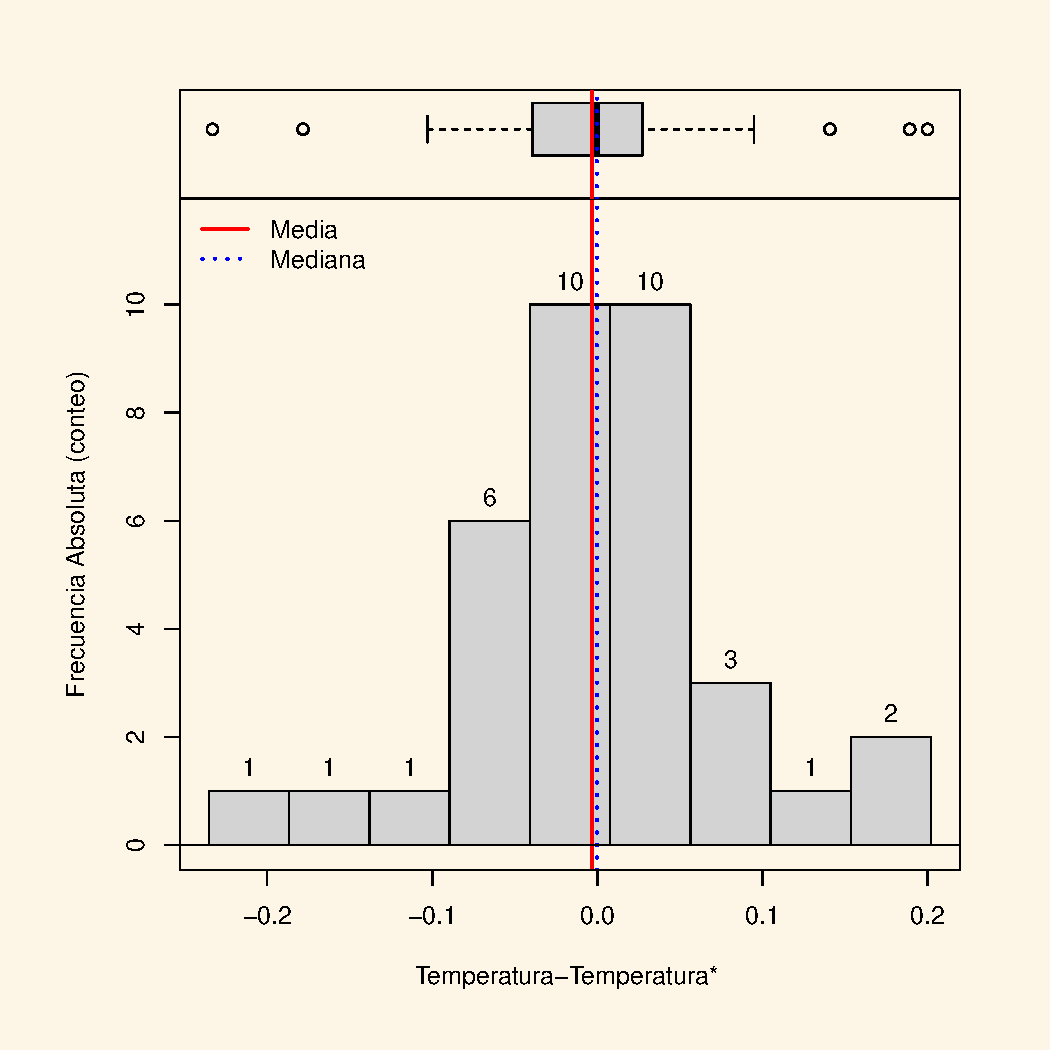
\includegraphics[width=0.75\linewidth]{Figuras_AED//VARIOGRAFICO/tem-tem+_HistBoxPlot1.pdf}
    \caption{Histograma y Boxplot de la diferencia (Z-Z*) Temperatura}
    \label{fig:enter-labelzx}
\end{figure}

 La Figura \ref{fig:enter-labelzx} combina un histograma y un boxplot para mostrar la variable "Temperatura-Temperatura*", que representa la diferencia entre dos conjuntos de mediciones de temperatura. El histograma de barras grises ilustra la frecuencia de las diferencias, con la mayoría de los datos concentrados en torno a cero, indicando que las predicciones del modelo son precisas. La media y la mediana, representadas por la línea roja y la línea de puntos azules respectivamente, también están cerca de cero, confirmando esta precisión. El boxplot, situado encima del histograma, muestra la dispersión de los datos y la mediana central, con puntos atípicos que sugieren algunas predicciones significativamente diferentes de las mediciones reales. Esta visualización es útil para evaluar rápidamente la variabilidad de los errores y la tendencia central de las diferencias, siendo valiosa para evaluar el rendimiento del modelo.



\begin{comment}
    

\subsubsection{Distribución espacial de las diferencias (Z-Z*) del parámetro temperatura}

\begin{figure}[!htb]
    \centering
    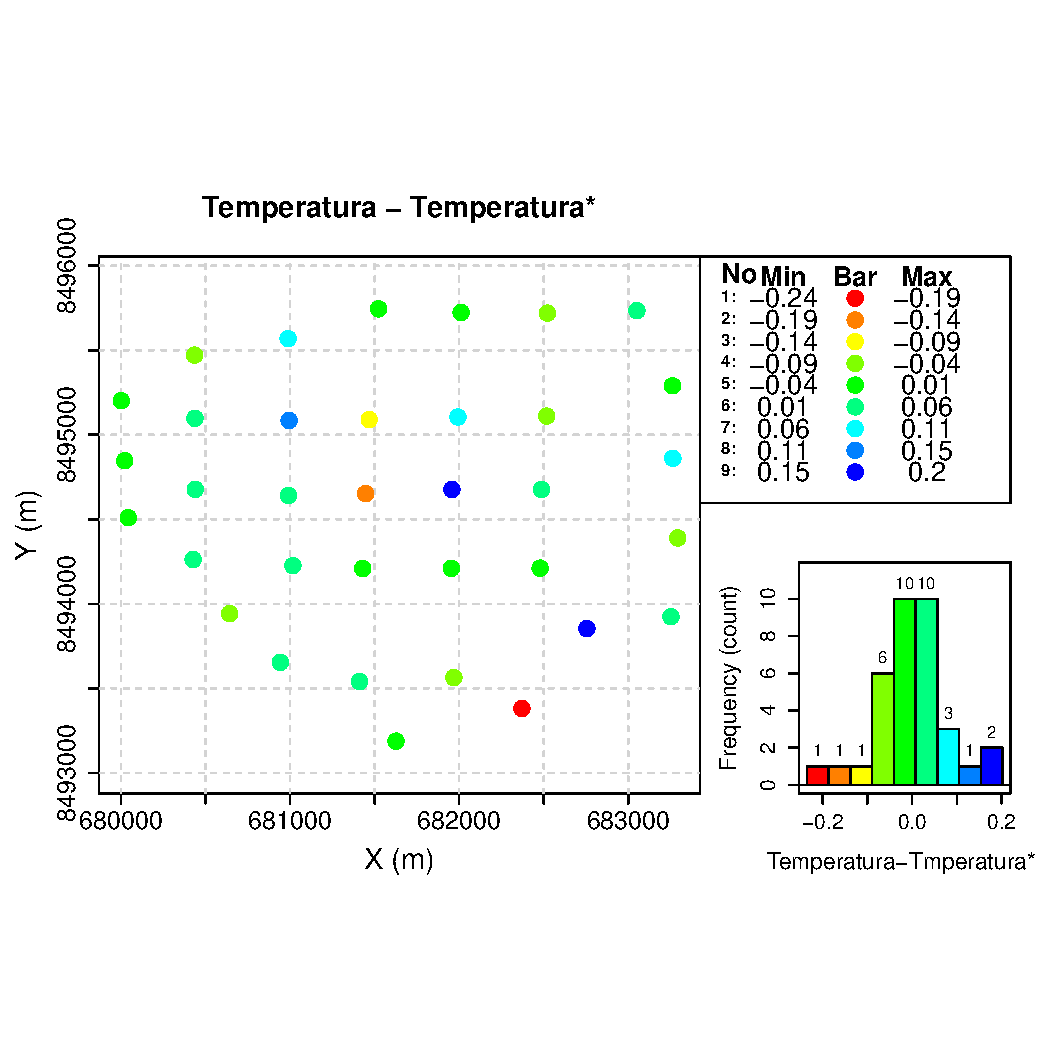
\includegraphics[width=0.8\linewidth]{Figuras_AED//VARIOGRAFICO/tem_CrossValid_Spatial_Distr.pdf}
    \caption{Distribución espacial de las diferencias (Z-Z*) para la Temperatura}
    \label{distrifinaltem}
\end{figure}

 La Figura \ref{distrifinaltem} ilustra la dispersión espacial de las variaciones entre dos series de datos, en concreto, ``Temperatura - Temperatura*'', que representa la disparidad propiamente dicha. Estas variaciones se representan mediante colores y se trazan en un plano bidimensional delimitado por las coordenadas ``X (m)'' e ``Y (m)''. Los puntos de color indican la magnitud de la disparidad en cada punto, acompañados de una leyenda situada en la parte superior derecha que asigna tonos a rangos específicos de variación, de -0,24 (rojo) a 0,20 (azul oscuro). El rojo denota las discrepancias más perjudiciales y el azul las más favorables. A la derecha, un minúsculo histograma muestra la frecuencia de estas discrepancias, con barras verticales en los tonos correspondientes que denotan el número de puntos dentro de cada rango de disparidades. El predominio de puntos verdes en el histograma sugiere que la mayoría de las discrepancias son próximas a cero, lo que implica una correlación espacial efectiva entre los dos conjuntos de datos de temperatura. Además, la distribución de los puntos en el gráfico no muestra un patrón discernible de agrupación o tendencia, lo que indica que las disparidades no están sistemáticamente conectadas con la ubicación. Este tipo de análisis es útil para señalar posibles zonas de disparidad entre las mediciones y las predicciones, así como para evaluar la homogeneidad del error en toda la zona examinada. En cuanto a los puntos rojos y azules que pueden sugerir o ser valores atípicos, puede observarse que los puntos rojos situados en los extremos podrían atribuirse a la ausencia de otro punto más extremo con el que asociarse; por lo tanto, es concebible que se encuentren dentro de los puntos de datos extremos.

\end{comment}

\subsection{Oxígeno Disuelto}
\subsubsection{Distribución espacial del Oxígeno Disuelto}
\begin{figure}[H]
    \centering
    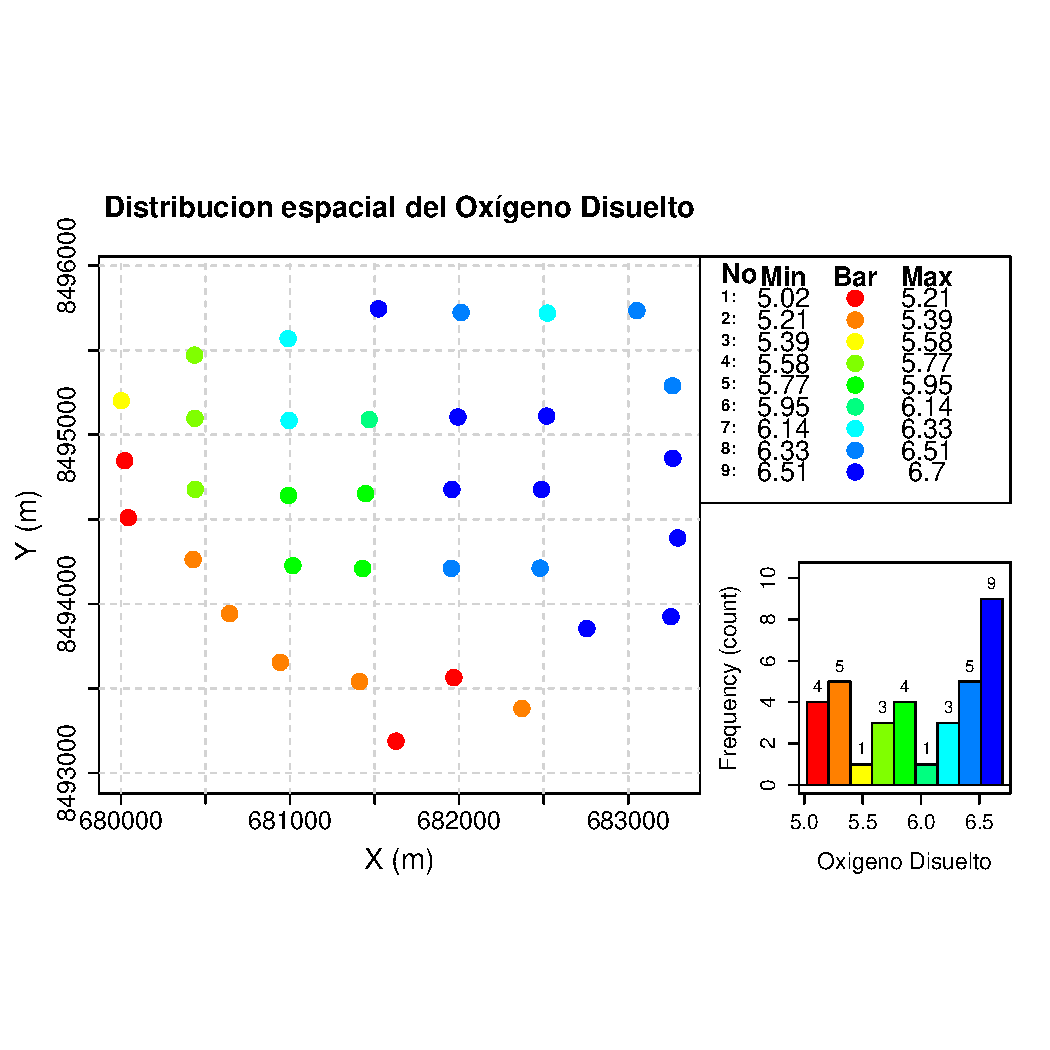
\includegraphics[width=0.8\linewidth]{Figuras_AED//VARIO_OD/od_Spatial_Distr.pdf}
    \caption{Distribución espacial del oxigeno disuelto}
    \label{fig:enter-labelCVC}
\end{figure}
La Figura \ref{fig:enter-labelCVC} muestra la distribución geográfica de las concentraciones de oxígeno disuelto mediante un gráfico de dispersión espacial, con coordenadas cartesianas X (m) e Y (m) que determinan las posiciones geográficas. Los puntos de datos están codificados por colores según una escala que va del rojo (concentraciones más bajas) al azul oscuro (concentraciones más altas). Un histograma incrustado en la esquina inferior derecha proporciona una perspectiva cuantitativa de la distribución de las concentraciones observadas, mostrando una variabilidad significativa con una tendencia hacia las concentraciones medias, destacada por la altura de las barras centrales.





\begin{comment}
    
\begin{figure}[!htb]
    \centering
    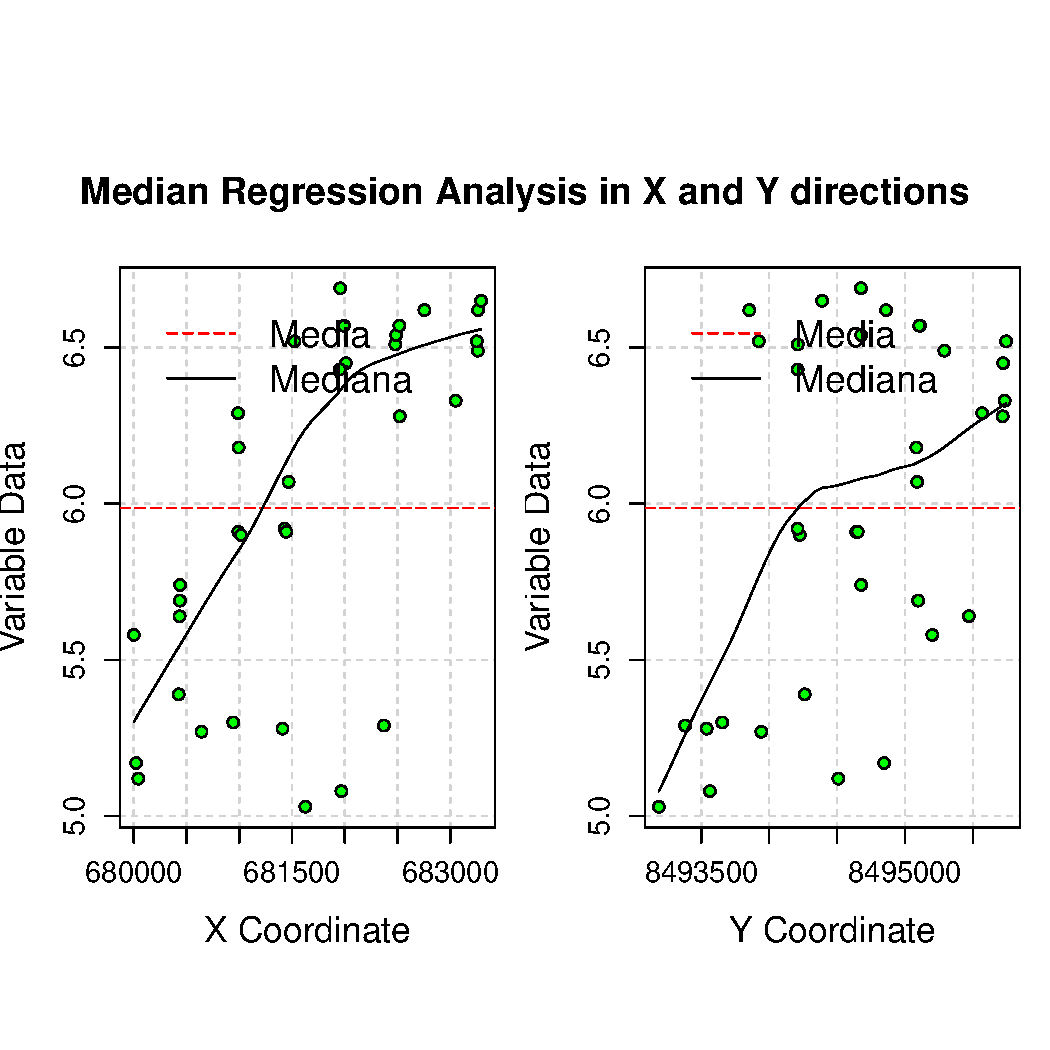
\includegraphics[width=0.7\linewidth]{Figuras_AED//VARIO_OD/od_Trend_X_Y.pdf}
    \caption{Análisis de regresión de la mediana en las direcciones X e Y para la variable Oxígeno Disuelto}
    \label{fig:enter-labelvt}
\end{figure}

  La Figura \ref{fig:enter-labelvt} presenta dos gráficos de análisis de regresión, uno para la dirección X y otro para la dirección Y, cuyo objetivo es examinar la relación entre la posición geográfica y las concentraciones de oxígeno disuelto. Estos gráficos se diseñaron para evaluar la estacionariedad espacial del parámetro, que se refiere a si la concentración de oxígeno disuelto cambia significativamente con la ubicación o permanece relativamente constante en todo el espacio muestreado. La estacionariedad espacial es un supuesto crítico en muchos modelos espaciales, y es esencial para la validez de las inferencias estadísticas sobre los datos. Las líneas de regresión trazadas a través de los puntos de datos proporcionan un ajuste medio, con las líneas rojas horizontales discontinuas representando la media y la mediana de las concentraciones de oxígeno disuelto. Si las líneas de regresión se ajustan estrechamente a los puntos de datos y las líneas horizontales se alinean con la tendencia central de los datos, esto sugeriría que no existe una tendencia espacial significativa y que las condiciones del oxígeno disuelto podrían considerarse estacionarias. Sin embargo, desviaciones significativas de estas líneas podrían indicar la presencia de gradientes o patrones espaciales que requieren un análisis más profundo, posiblemente utilizando técnicas de modelización espacial como kriging o interpolación espacial para comprender mejor la variabilidad espacial del oxígeno disuelto en la zona de estudio.

\end{comment}

  \subsubsection{Modelización univariante de la variografía Oxígeno Disuelto }
\begin{enumerate}
    \item \subsubsection{Variogramas direccionales en 4 direcciones (0, 45, 90 y 135)}

\begin{figure}[!htb]
    \centering
    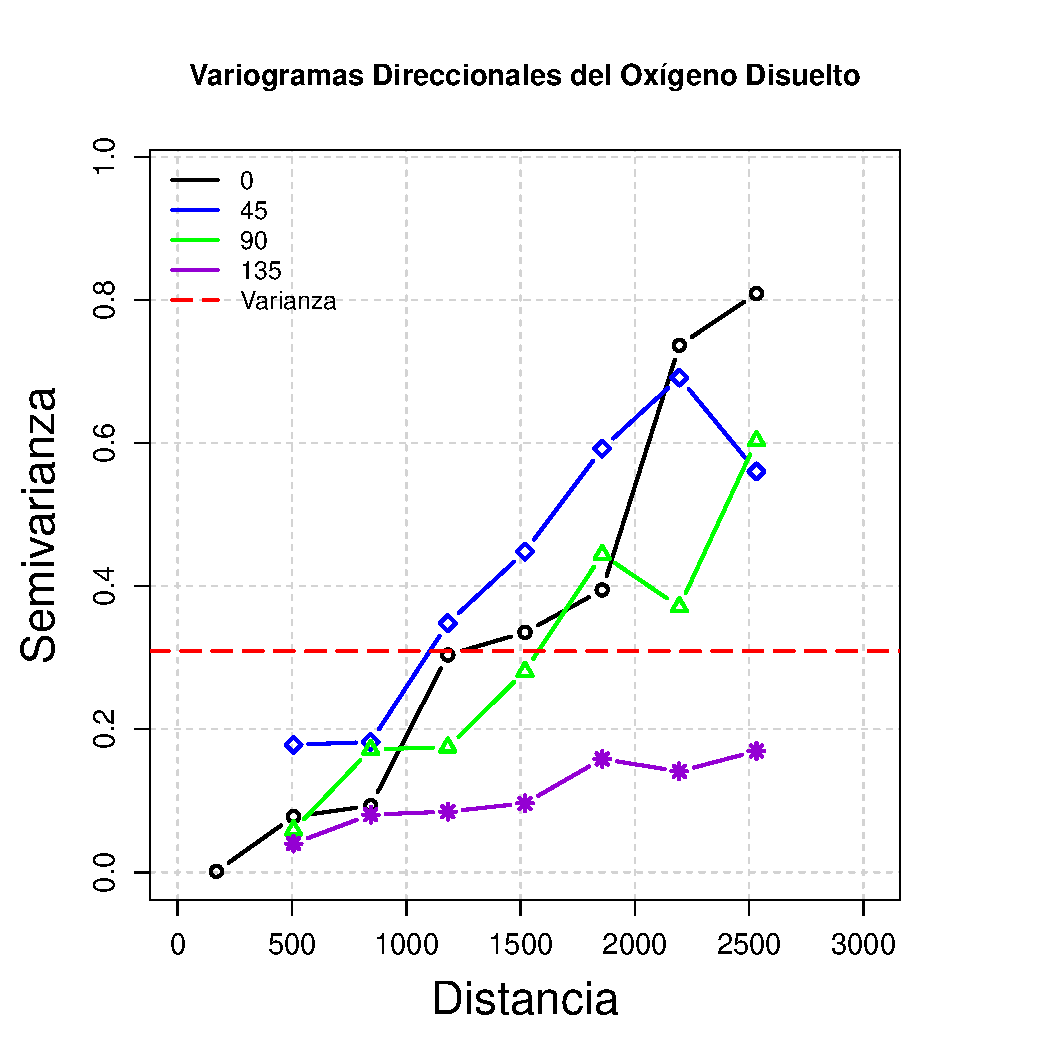
\includegraphics[width=0.8\linewidth]{Figuras_AED//VARIO_OD/OD_Vario4DEstimation.pdf}
    \caption{Análisis comparativo de variogramas direccionales para el Oxigeno Disuelto}
    \label{fig:enter-labelxfg}
\end{figure}

La Figura \ref{fig:enter-labelxfg} presenta variogramas direccionales para el oxígeno disuelto, mostrando la semivarianza frente a la distancia en diferentes direcciones (0°, 45°, 90°, 135°) para evaluar la anisotropía espacial. La línea roja discontinua indica la varianza total, y los resultados sugieren que la semivarianza aumenta con la distancia, reflejando una disminución de la similitud espacial. Las direcciones 0° muestran mayor continuidad, mientras que 90° y 135° exhiben mayores aumentos de semivarianza. La anisotropía observada podría justificar el uso de modelos anisotrópicos, pero se opta por variogramas isotrópicos debido a la homogeneidad de la Laguna de Pacucha y la fuerte correlación entre temperatura y oxígeno disuelto. Este enfoque isotrópico facilitará el uso de técnicas de cokriging para obtener estimaciones precisas y coherentes de ambos parámetros ambientales.


\item \subsubsection{Ajuste automático del modelo de variograma para el Oxígeno Disuelto}
\begin{figure}[!htb]
    \centering
    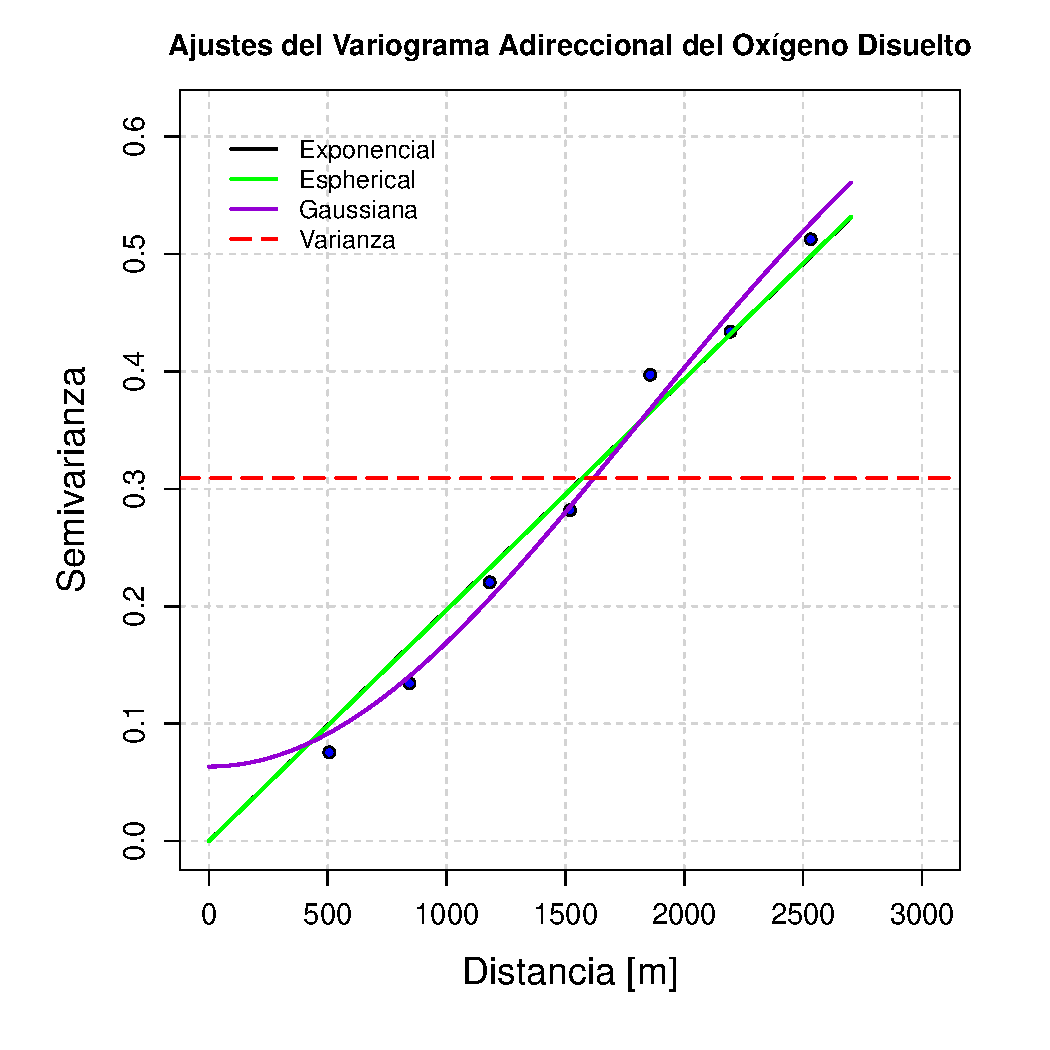
\includegraphics[width=0.8\linewidth]{Figuras_AED//VARIO_OD/OD_VarioAllModelEstimation.pdf}
    \caption{Ajustes de los variogramas modelos para el Oxígeno Disuelto }
    \label{fig:enter-labelnh}
\end{figure}

La Figura \ref{fig:enter-labelnh} muestra un variograma direccional del oxígeno disuelto, con la distancia en el eje horizontal y la semivarianza en el eje vertical. Incluye tres modelos teóricos: el exponencial (línea continua negra), el esférico (línea punteada verde) y el gaussiano (línea moteada morada), junto con los puntos azules que representan las semivarianzas empíricas y la línea roja discontinua que indica la varianza total. Este gráfico es crucial en geoestadística para seleccionar el modelo de variograma más adecuado, lo cual impacta la calidad de las interpolaciones espaciales como el kriging, permitiendo evaluar visualmente el ajuste de los modelos a los datos empíricos.



 \item \subsubsection{Ajuste manual y óptimo del modelo de variograma para el Oxígeno Disuelto}
 
\begin{figure}[!htb]
    \centering
    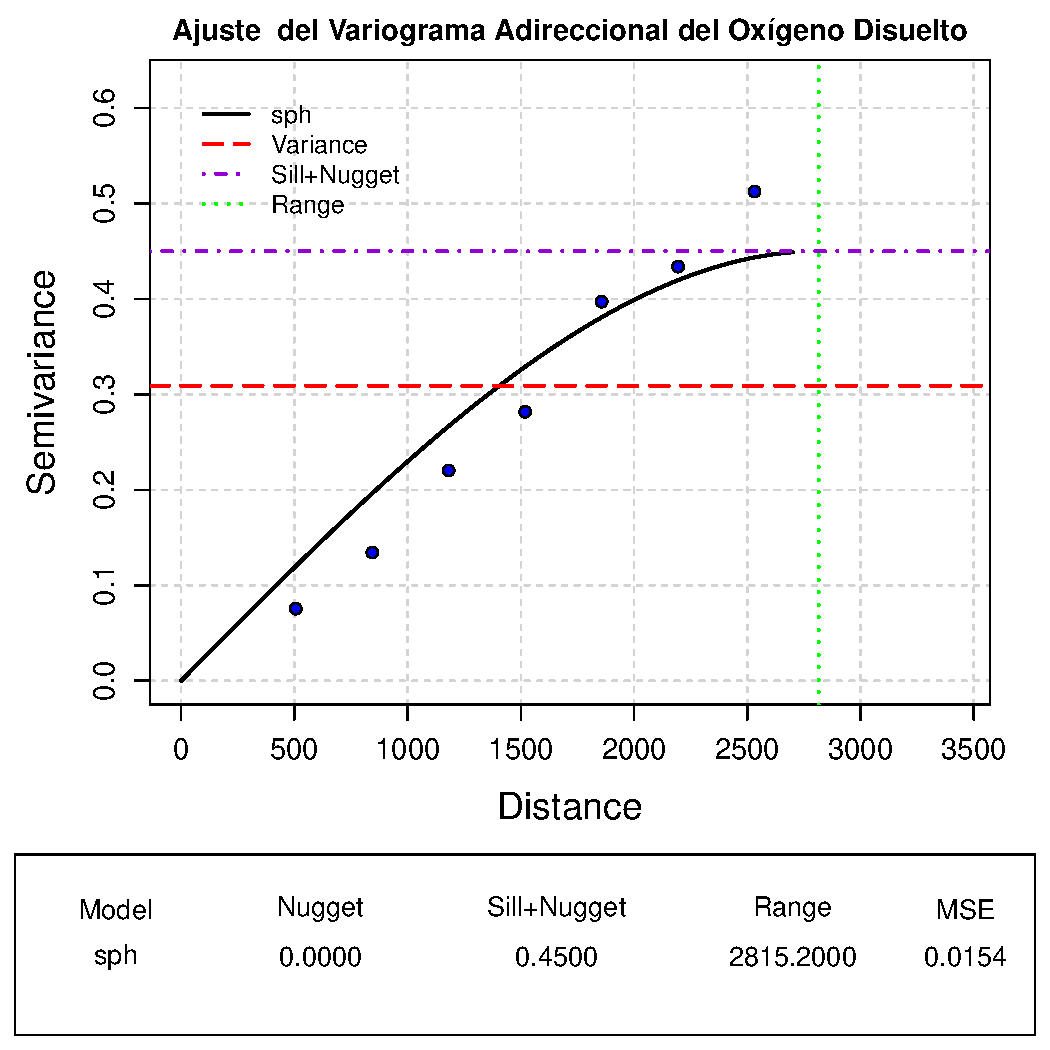
\includegraphics[width=0.8\linewidth]{Figuras_AED//VARIO_OD/od_VarioEyeEstimation.pdf}
    \caption{ Optimización  del Modelo Esférico del Variograma Oxígeno Disuelto}
    \label{fig:enter-labelqwwe}
\end{figure}

La Figura \ref{fig:enter-labelqwwe} muestra un ajuste variográfico direccional, con la semivarianza en función de la distancia. El modelo esférico (sph), representado por una línea negra continua, alcanza una meseta que indica el umbral de variabilidad, mostrado por la línea roja discontinua. La línea morada horizontal en el origen indica una pepita de 0,0000, sugiriendo ausencia de variabilidad aleatoria. La línea verde vertical discontinua marca el rango del variograma, aproximadamente 2815,200 metros, más allá del cual los datos no están correlacionados. Los puntos azules representan semivarianzas empíricas. Con un MSE de 0,0154, el modelo esférico proporciona un buen ajuste a los datos empíricos, esencial para la interpolación espacial mediante kriging y crucial para comprender la estructura espacial de la variable y predecir sus valores en ubicaciones no muestreadas.




\end{enumerate}
 \subsubsection{Validación cruzada del modelo de variograma esférico para el Oxígeno Disuelto}


\begin{table}[!htb]
\centering
\caption{Validación cruzada del modelo esférico para el Oxígeno Disuelto}
\label{tab:oxigeno_disuelto}
\begin{tabular}{ccccc}
\hline
X (m) & Y (m) & Z & Z* & Z-Z* \\ \hline
682370.9 & 8493381 & 5.29 & 5.601986 & -0.311986 \\
681968.2 & 8493564 & 5.08 & 5.494456 & -0.414456 \\
681626.5 & 8493188 & 5.03 & 5.061755 & -0.031755 \\
681410.7 & 8493540 & 5.28 & 5.248302 & 0.031698 \\
680942.6 & 8493654 & 5.30 & 5.309175 & -0.009175 \\
680642.8 & 8493942 & 5.27 & 5.420541 & -0.150541 \\
680426.7 & 8494262 & 5.39 & 5.398255 & -0.008255 \\
680043.0 & 8494509 & 5.12 & 5.284912 & -0.164912 \\
680022.2 & 8494846 & 5.17 & 5.402581 & -0.232581 \\
680001.5 & 8495201 & 5.58 & 5.325449 & 0.254551 \\
680435.0 & 8495471 & 5.64 & 5.885293 & -0.245293 \\
680437.3 & 8495097 & 5.69 & 5.713575 & -0.023575 \\
680438.9 & 8494677 & 5.74 & 5.496993 & 0.243007 \\
680991.1 & 8494641 & 5.91 & 5.939384 & -0.029384 \\
681016.2 & 8494226 & 5.90 & 5.649100 & 0.250900 \\
681429.4 & 8494209 & 5.92 & 5.919327 & 0.000673 \\
681446.3 & 8494652 & 5.91 & 6.182906 & -0.272906 \\
681468.0 & 8495090 & 6.07 & 6.330617 & -0.260617 \\
680994.2 & 8495084 & 6.18 & 5.997984 & 0.182016 \\
680988.5 & 8495568 & 6.29 & 6.125942 & 0.164058 \\
681523.6 & 8495745 & 6.52 & 6.331416 & 0.188584 \\
682011.0 & 8495723 & 6.45 & 6.433230 & 0.016770 \\
682521.8 & 8495719 & 6.28 & 6.421860 & -0.141860 \\
683051.2 & 8495734 & 6.33 & 6.282751 & 0.047249 \\
683261.6 & 8495290 & 6.49 & 6.482177 & 0.007823 \\
683263.4 & 8494861 & 6.62 & 6.588642 & 0.031358 \\
683292.6 & 8494390 & 6.65 & 6.619040 & 0.030960 \\
683252.4 & 8493924 & 6.52 & 6.556798 & -0.036798 \\
682755.0 & 8493854 & 6.62 & 6.183957 & 0.436043 \\
682478.8 & 8494211 & 6.51 & 6.552490 & -0.042490 \\
682486.6 & 8494677 & 6.54 & 6.702482 & -0.162482 \\
682517.5 & 8495110 & 6.57 & 6.577609 & -0.007609 \\
681992.6 & 8495105 & 6.57 & 6.510776 & 0.059224 \\
681957.2 & 8494676 & 6.69 & 6.419097 & 0.270903 \\
681954.0 & 8494210 & 6.43 & 6.136216 & 0.293784 \\ \hline
\end{tabular}
\end{table}

La Tabla \ref{tab:oxigeno_disuelto} muestra los resultados de la validación cruzada del modelo esférico para el variograma del oxígeno disuelto, evaluando la precisión del modelo geoestadístico al comparar valores observados (\textit{Z}) y estimados (\textit{Z*}) en 35 puntos de muestreo. La diferencia (\textit{Z-Z*}) promedio cercana a cero indica la ausencia de sesgo sistemático y valida la capacidad predictiva del modelo. Este análisis es crucial para verificar la eficacia del modelo en diversos lugares y puede revelar patrones o tendencias que sugieran mejoras en el modelo o la técnica de muestreo. Un análisis detallado adicional podría implicar la homogeneidad de las varianzas, autocorrelación espacial o factores ambientales externos, esenciales para comprender la dinámica del oxígeno disuelto en la Laguna de Pacucha y optimizar futuros modelos predictivos.

 
\subsubsection{Estadísticos de la validación cruzada para el modelo esférico para el Oxigeno Disuelto}

\begin{table}[!htb]
\centering
\caption{Estadísticos descriptivos de la validación cruzada para oxígeno disuelto.}
\label{tab:cross_vvalidation}
\begin{tabular}{
  l
  S
  S
  S[table-format=-1.5] % Columna para números negativos
}
\toprule
{Estadístico} & {Z} & {Z*} & {Z-Z*} \\
\midrule
No muestras        & 35.00000 & 35.00000 & 35.00000 \\
Mínimo             & 5.03000  & 5.06176  & -0.41446 \\
Cuartil 1er        & 5.48500  & 5.49572  & -0.14620 \\
Mediana            & 6.07000  & 6.12594  & -0.00761 \\
Media              & 5.98714  & 5.98820  & -0.00106 \\
Cuartil 3er        & 6.51500  & 6.42754  & 0.11164  \\
Máximo             & 6.69000  & 6.70248  & 0.43604  \\
Rango              & 1.66000  & 1.64073  & 0.85050  \\
Rango Intercuartil & 1.03000  & 0.93182  & 0.25784  \\
Varianza           & 0.30913  & 0.24829  & 0.03733  \\
Desv Estándar      & 0.55600  & 0.49829  & 0.19321  \\
Simetría           & -0.34761 & -0.25545 & 0.05880  \\
Curtosis           & 1.64106  & 1.64298  & 2.64740  \\
\bottomrule
\end{tabular}
\end{table}

El análisis descriptivo basado en 35 muestras de la concentración de oxígeno disuelto Tabla \textbf{\ref{tab:cross_vvalidation}} revela que, aunque el modelo subestima ligeramente el mínimo observado (Z), las medidas centrales de tendencia y dispersión, como la mediana y el rango intercuartil de las diferencias (Z-Z*), sugieren que las estimaciones del modelo (Z*) están en general alineadas con los valores observados. La media cercana a cero en las diferencias indica una buena precisión del modelo, mientras que la distribución sesgada y la curtosis mayor que uno reflejan una distribución con colas más pesadas, señalando la presencia de algunos valores extremos. Estos hallazgos sugieren que, aunque el modelo proporciona estimaciones razonables de la concentración de oxígeno disuelto, las desviaciones en las diferencias podrían ser un foco para futuras mejoras del modelo.

\begin{figure}[!htb]
    \centering
    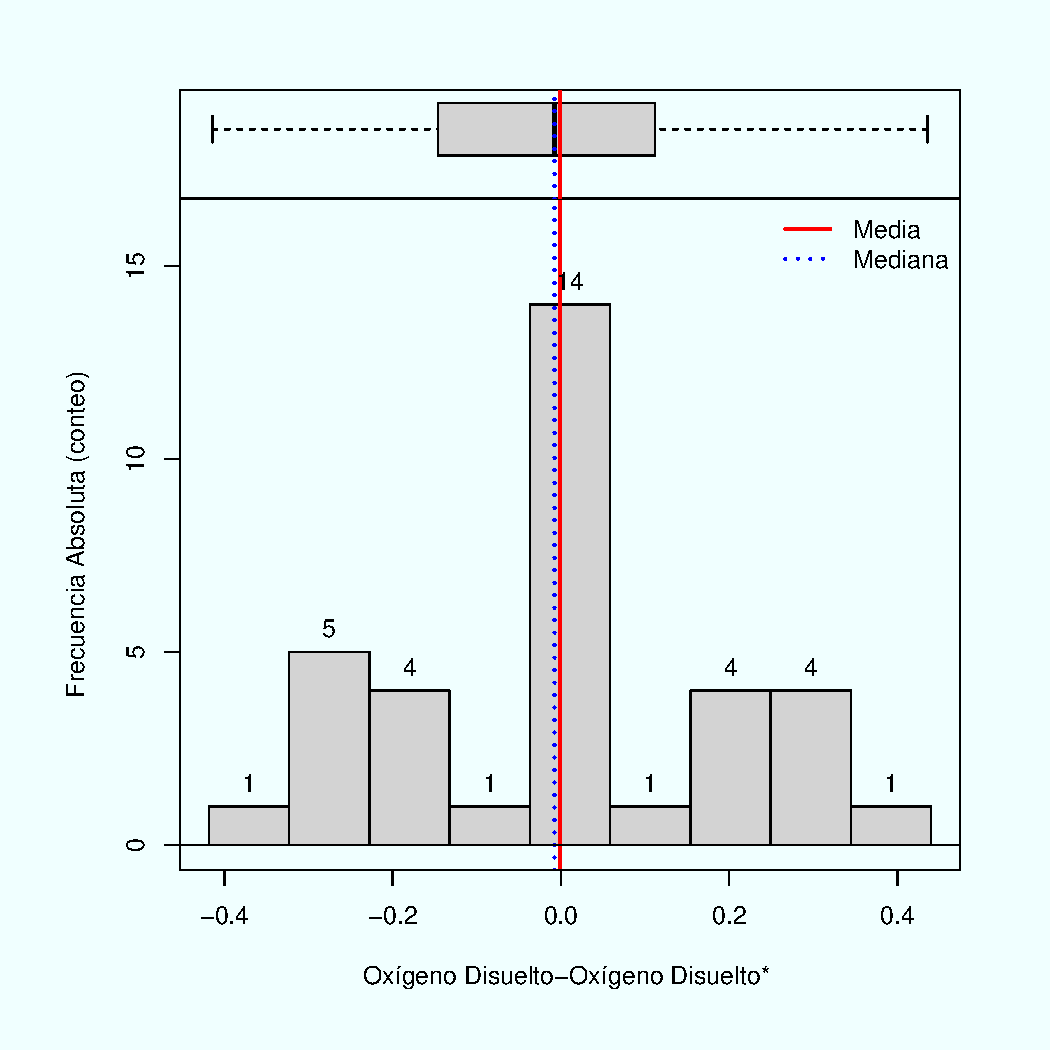
\includegraphics[width=0.6\linewidth]{Figuras_AED//VARIO_OD/OD-OD+_HistBoxPlot1.pdf}
    \caption{Histograma y Boxplot de la diferencia (Z-Z*)  Oxigeno Disuelto}
    \label{fig:enter-labee4l}
\end{figure}


 La Figura \ref{fig:enter-labee4l} presenta un diagrama de caja y un histograma superpuestos que muestran la distribución de las diferencias entre los valores observados y estimados de oxígeno disuelto. El histograma indica que estas diferencias se concentran principalmente en torno a cero, con la barra más alta mostrando una frecuencia de 14, lo que sugiere alta precisión en las estimaciones. El boxplot revela que la mediana y la media de las diferencias están cerca de cero, evidenciando la ausencia de sesgo sistemático. Además, el rango intercuartílico del boxplot es simétrico alrededor de cero, reflejando coherencia en la variabilidad de las diferencias. La ausencia de valores atípicos en el boxplot confirma que el modelo de estimación de oxígeno disuelto es fiable y proporciona predicciones consistentes dentro del rango esperado.



\begin{comment}
    

\subsubsection{Distribución espacial de las diferencias (Z-Z*) del parámetro Oxigeno Disuelto }

\begin{figure}[!htb]
    \centering
    \includegraphics[width=0.8\linewidth]{Figuras_AED//VARIO_OD/Oxígeno_Disuelto_CrossValid_Spatial_Distr.pdf}
    \caption{Distribución espacial de las diferencias (Z-Z*) para el Oxígeno Disuelto}
    \label{fig:enter-labeldy}
\end{figure}

 La Figura \ref{fig:enter-labeldy} muestra un diagrama de dispersión que aclara la distribución espacial de las disparidades entre las concentraciones de oxígeno disuelto observadas y estimadas. Las coordenadas ``X (m)'' e ``Y (m)'' delinean la ubicación geográfica de cada muestra en el espacio, y los puntos están codificados por colores para representar el rango de diferencias de concentración. La leyenda indica los valores mínimo, máximo y asociado de cada color.
La leyenda indica los valores mínimo, máximo y asociado de cada color.

La distribución espacial de los colores demuestra la variación en las diferencias entre las concentraciones observadas y estimadas de oxígeno disuelto. Los puntos más cercanos al centro indican una buena concordancia entre las concentraciones observadas y estimadas, mientras que los puntos más alejados del centro significan mayores discrepancias. La concentración de puntos en el centro sugiere que el modelo de estimación predijo con exactitud las concentraciones de oxígeno disuelto en la mayoría de los lugares.

El histograma de la esquina inferior derecha del gráfico representa la frecuencia absoluta de estas diferencias en intervalos específicos. La barra más alta corresponde al intervalo que incluye el cero, lo que indica que la mayor frecuencia de diferencias es aproximadamente cero y que la mayoría de las estimaciones son precisas. Las barras de los demás colores representan las frecuencias de diferencias más significativas, tanto positivas como negativas.

En resumen, el diagrama de dispersión y el histograma proporcionan una comprensión global de la precisión del modelo en el espacio geográfico, permitiendo identificar cualquier tendencia espacial en los errores de estimación y la uniformidad de las diferencias en la región estudiada.

\end{comment}



\subsection{pH}
\subsubsection{Distribución espacial del pH}
\begin{figure}[!htb]
    \centering
    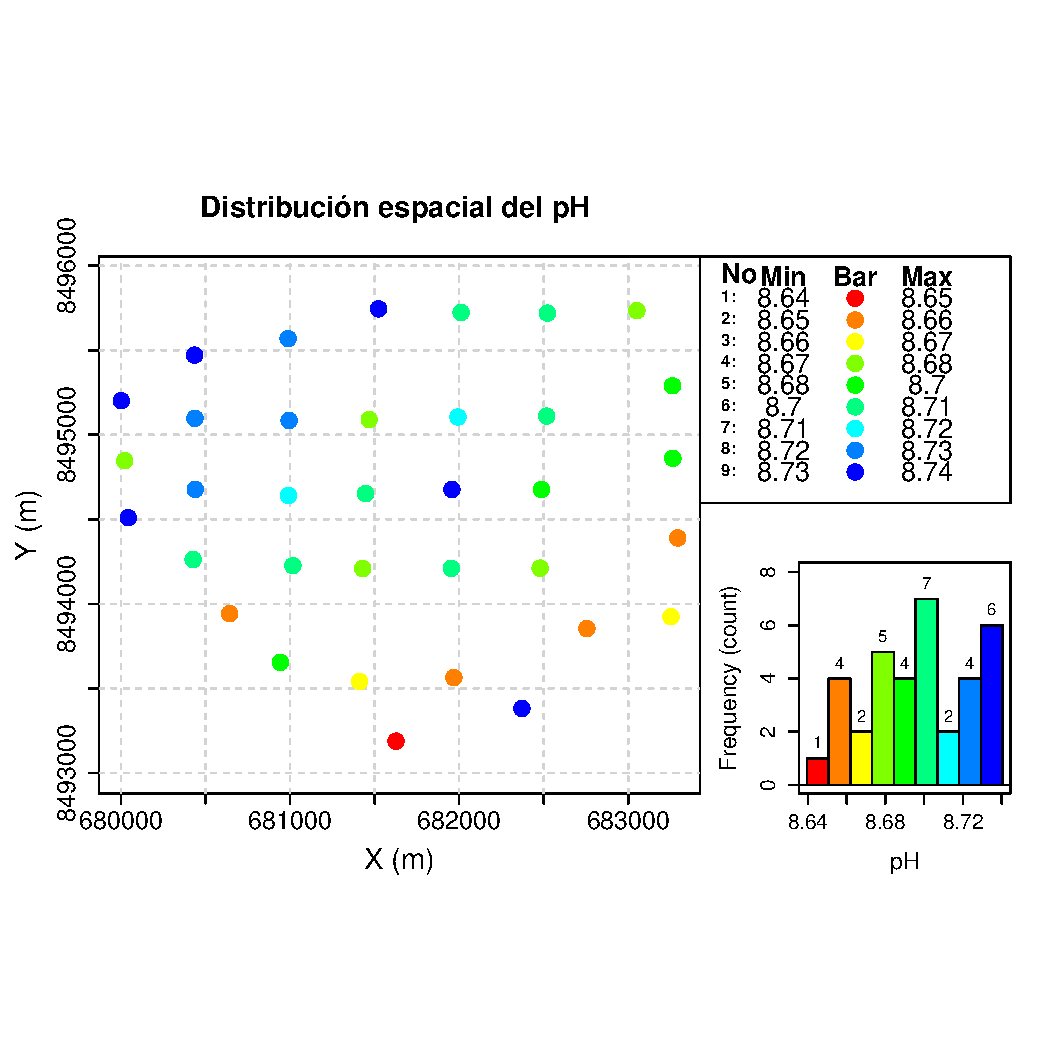
\includegraphics[width=0.8\linewidth]{Figuras_AED//PH/tem_Spatial_Distr.pdf}
    \caption{Distribución espacial del pH en la laguna de Pacucha}
    \label{fig:enter-labeldis}
\end{figure}


\begin{comment}
    \begin{figure} [!htb]
    \centering
    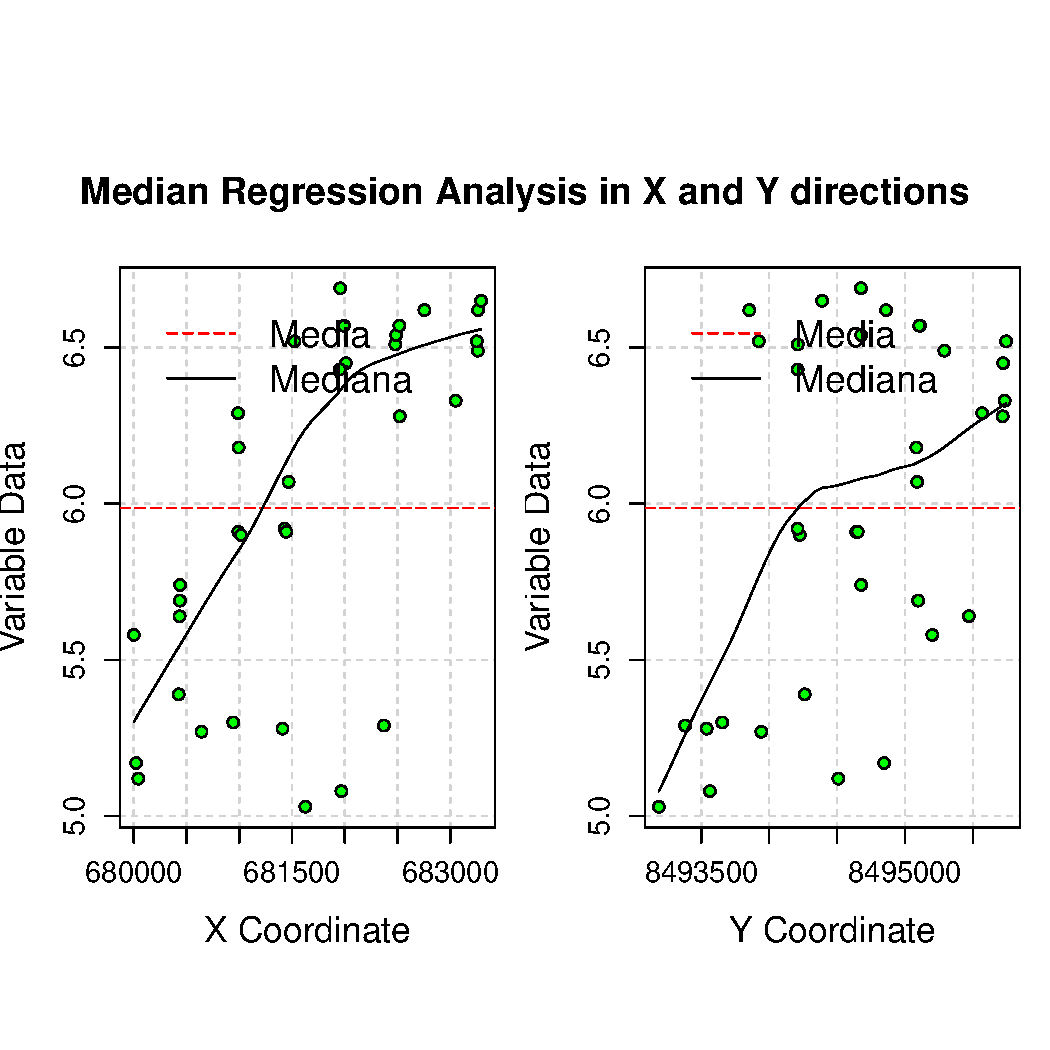
\includegraphics[width=0.6\linewidth]{Figuras_AED//VARIO_OD/od_Trend_X_Y.pdf}
    \caption{Análisis de regresión de la mediana en las direcciones X e Y para la variable pH}
    \label{fig:enter-labelqw}
\end{figure}
\end{comment}

 La distribución espacial del pH en la Laguna Pacucha fue examinada identificando valores extremos en un gráfico de dispersión Figura \ref{fig:enter-labeldis} . Estos están representados por puntos que están significativamente distantes del rango de valores comúnmente observados, como lo indican los colores en la leyenda. Estas muestras requieren atención especial para determinar si representan condiciones anómalas reales, variabilidad natural o errores en la recolección o análisis de datos.

\begin{comment}
    En cuanto a la regresión de la mediana Figura \ref{fig:enter-labelqw}, los valores extremos se refieren a puntos que se desvían significativamente de la línea de regresión, lo que indica que el valor del pH en ese lugar concreto es mucho mayor o menor que el observado en lugares con coordenadas similares. Estas desviaciones pueden indicar zonas dentro de la laguna que tienen características químicas distintas, que podrían ser de interés para estudios ecológicos y de conservación.
\end{comment}





\subsubsection{Modelización univariante de la variografía del pH}

\begin{enumerate}
    \item Variogramas direccionales en 4 direcciones (0, 45, 90 y 135)

\begin{figure}[!htb]
    \centering
    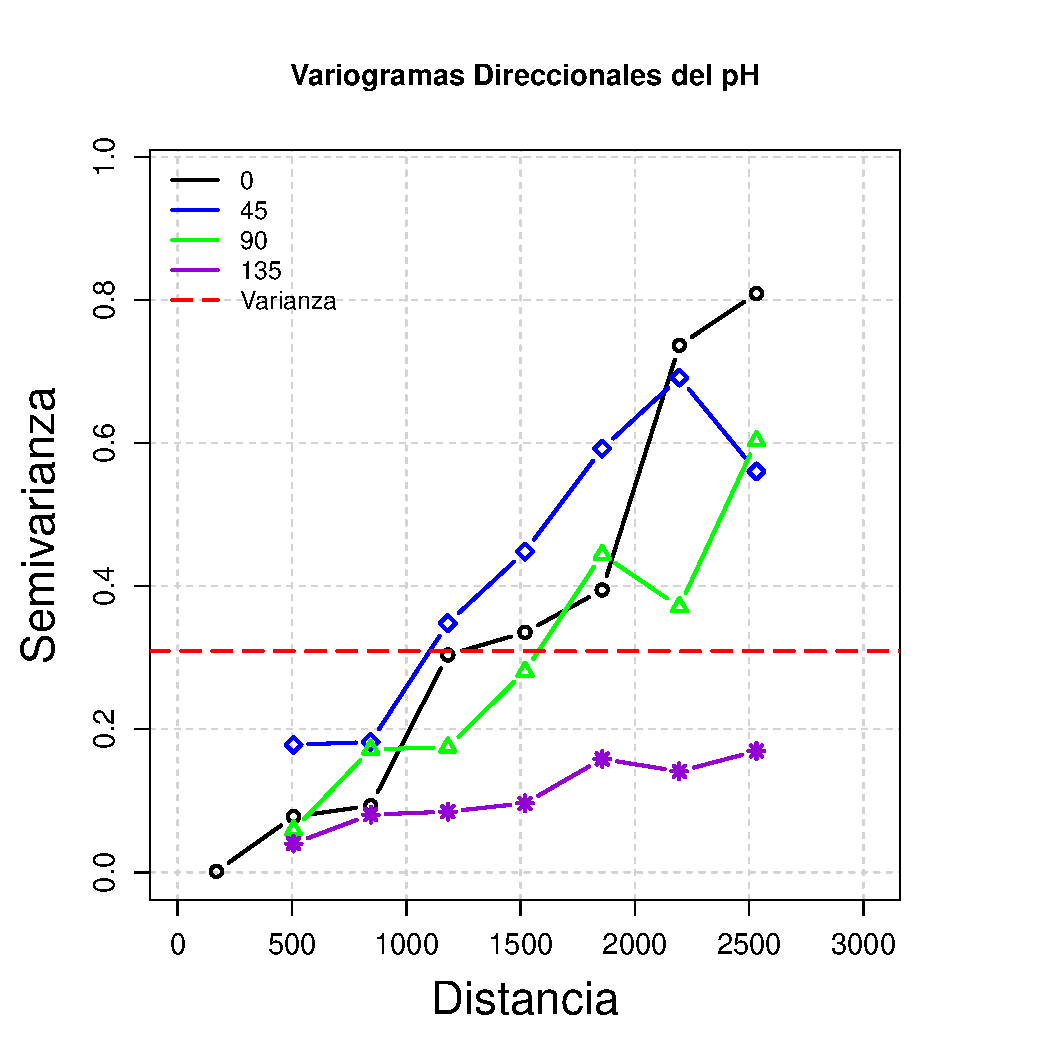
\includegraphics[width=0.85\linewidth]{Figuras_AED//PH/ph_Vario4DEstimation.pdf}
    \caption{Análisis comparativo de variogramas direccionales para el pH}
    \label{fig:enter-label4d}
\end{figure}

La Figura \ref{fig:enter-label4d} muestra variogramas direccionales del pH, representando la semivarianza en función de la distancia en ángulos de 0, 45, 90 y 135 grados. La línea negra (0 grados) indica una posible anisotropía al mostrar una tendencia diferente. Las líneas azul (45 grados) y púrpura (135 grados) revelan un aumento más rápido de la semivarianza con la distancia, mientras que la línea verde (90 grados) muestra un incremento menos pronunciado. La línea roja discontinua indica la varianza total del pH, crucial para identificar el sill. Evaluar estos variogramas es esencial para determinar la anisotropía y seleccionar el variograma teórico adecuado, lo cual es vital para la interpolación precisa mediante kriging en la Laguna de Pacucha.



\item Mejor ajuste automático del modelo de variograma para la temperatura
\begin{figure}[!htb]
    \centering
    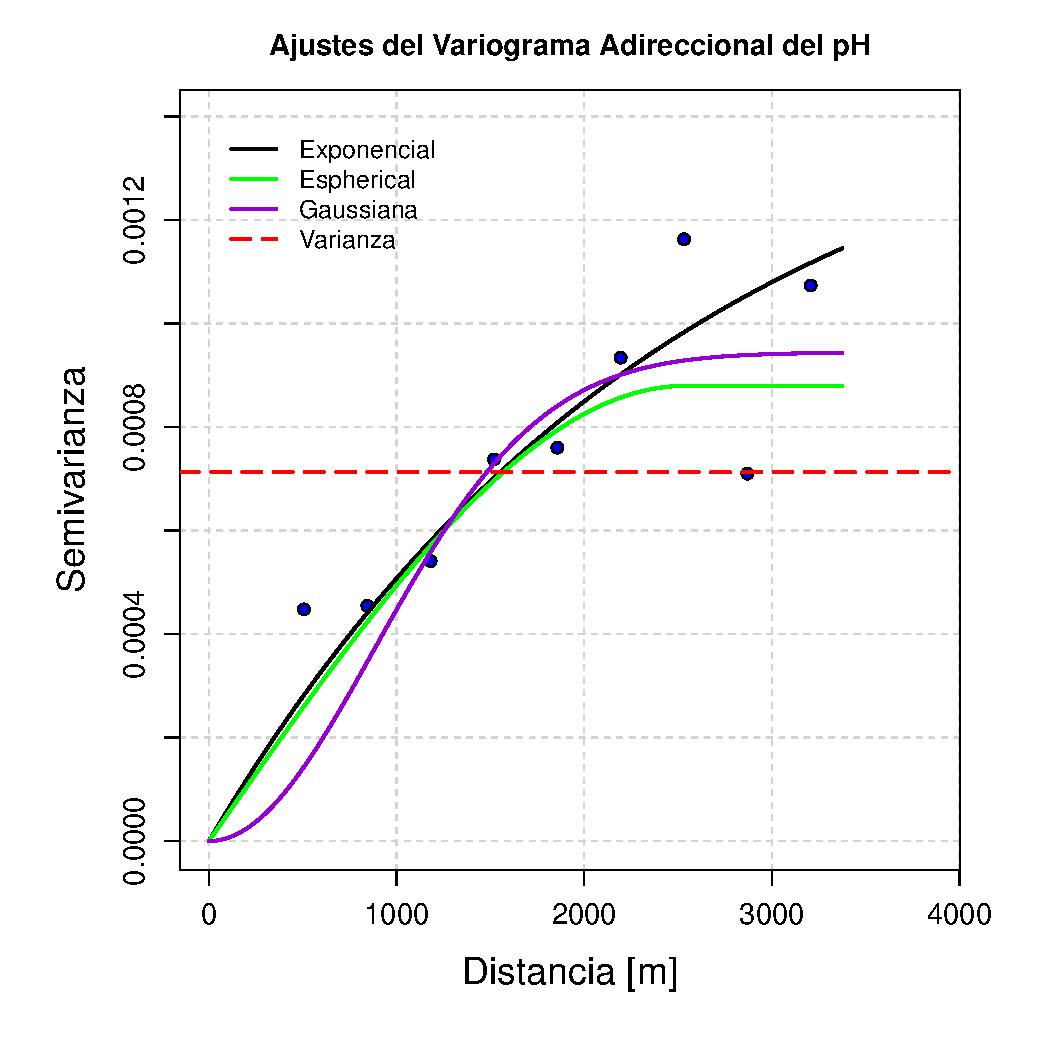
\includegraphics[width=0.8\linewidth]{Figuras_AED/VARIOGRAFICO/ph_VarioAllModelEstimation.pdf}
    \caption{Mejor modelo de variograma ajustado  para el pH}
    \label{fig:enter-labelcer}
\end{figure}

 La Figura \ref{fig:enter-labelcer} muestra un variograma adireccional ajustado para el pH, con la distancia en metros en el eje horizontal y la semivarianza en el eje vertical. Los puntos azules representan la semivarianza calculada a diferentes distancias. Se ajustaron tres modelos teóricos: esférico (línea marrón punteada), exponencial (línea verde sólida) y gaussiano (línea morada sólida). La línea roja punteada indica la varianza total del pH. El modelo esférico y el gaussiano muestran un incremento más suave de la semivarianza con la distancia, mientras que el exponencial muestra un aumento más pronunciado en distancias cortas. Este análisis es esencial para entender la estructura espacial del pH y seleccionar el modelo adecuado para la interpolación mediante kriging, afectando directamente la precisión de las estimaciones de pH en ubicaciones no muestreadas.


\item Ajuste manual y óptimo del modelo de variograma para el pH
\begin{figure}[!htb]
    \centering
    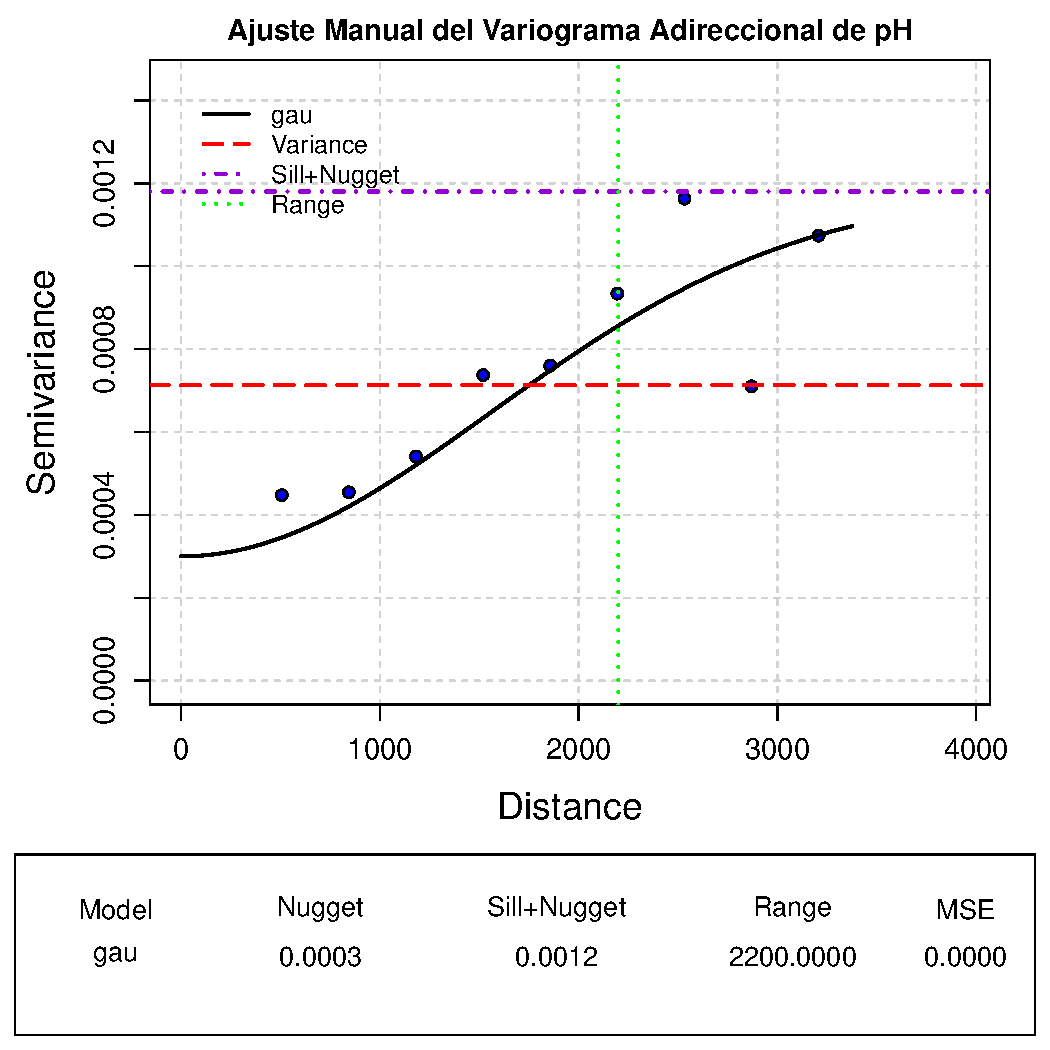
\includegraphics[width=0.8\linewidth]{Figuras_AED/VARIOGRAFICO/ph_VarioEyeEstimation.pdf}
    \caption{ Optimización Manual del Modelo Esférico para el  Variograma del pH}
    \label{fig:enter-labeldezxc}
\end{figure}

La Figura \ref{fig:enter-labeldezxc} muestra un variograma experimental adireccional de pH ajustado con un modelo teórico gaussiano. Los puntos azules representan la semivarianza calculada para distintas distancias, mientras que la línea negra muestra el modelo gaussiano ajustado. El rango, indicado por la línea vertical punteada verde, es de aproximadamente 2200 unidades, donde la semivarianza se estabiliza en el sill (línea roja punteada) más el efecto pepita (línea morada punteada). El nugget es 0.0003, el sill más nugget es 0.0012, y el error cuadrático medio (MSE) es 0.0000, indicando un ajuste preciso. Estos resultados sugieren una correlación espacial del pH hasta 2200 unidades, más allá de las cuales no hay dependencia espacial significativa.

 
\end{enumerate}

\subsubsection{Validación cruzada del modelo de variograma esférico para el pH}
\begin{table}[H]
\centering
\caption{Resultados de la validación cruzada para pH}
\label{tab:cross_validation_pH}
\begin{tabular}{cccccc}
\hline
\textbf{Nº} & \textbf{X} & \textbf{Y} & \textbf{Z (Observado)} & \textbf{Z* (Estimado)} & \textbf{Z-Z* (Diferencia)} \\ \hline
1 & 682370.9 & 8493381 & 8.74 & 8.653691 & 0.086309354 \\
2 & 681968.2 & 8493564 & 8.64 & 8.681199 & -0.041199371 \\
3 & 681626.5 & 8493188 & 8.64 & 8.678733 & -0.038733147 \\
4 & 681410.7 & 8493540 & 8.67 & 8.674090 & -0.004089855 \\
5 & 680942.6 & 8493654 & 8.69 & 8.672867 & 0.017133460 \\
6 & 680642.8 & 8493942 & 8.66 & 8.691379 & -0.031378781 \\
7 & 680426.7 & 8494262 & 8.70 & 8.696148 & 0.003852306 \\
8 & 680043.0 & 8494509 & 8.73 & 8.700733 & 0.029267267 \\
9 & 680022.2 & 8494846 & 8.68 & 8.721390 & -0.041389855 \\
10 & 680001.5 & 8495201 & 8.73 & 8.717077 & 0.012923210 \\
11 & 680435.0 & 8495471 & 8.73 & 8.721927 & 0.008072903 \\
12 & 680437.3 & 8495097 & 8.72 & 8.717804 & 0.002195732 \\
13 & 680438.9 & 8494677 & 8.72 & 8.708551 & 0.011449012 \\
14 & 680991.1 & 8494641 & 8.71 & 8.703625 & 0.006374860 \\
15 & 681016.2 & 8494226 & 8.70 & 8.690734 & 0.009265608 \\
16 & 681429.4 & 8494209 & 8.68 & 8.691058 & -0.011058195 \\
17 & 681446.3 & 8494652 & 8.70 & 8.702611 & -0.002610860 \\
18 & 681468.0 & 8495090 & 8.68 & 8.715911 & -0.035910774 \\
19 & 680994.2 & 8495084 & 8.72 & 8.715408 & 0.004591598 \\
20 & 680988.5 & 8495568 & 8.72 & 8.723182 & -0.003181674 \\
21 & 681523.6 & 8495745 & 8.74 & 8.711467 & 0.028533499 \\
22 & 682011.0 & 8495723 & 8.70 & 8.713385 & -0.013384691 \\
23 & 682521.8 & 8495719 & 8.70 & 8.701045 & -0.001044871 \\
24 & 683051.2 & 8495734 & 8.68 & 8.696412 & -0.016411739 \\
25 & 683261.6 & 8495290 & 8.69 & 8.682301 & 0.007698617 \\
26 & 683263.4 & 8494861 & 8.69 & 8.677674 & 0.012325671 \\
27 & 683292.6 & 8494390 & 8.66 & 8.682694 & -0.022693628 \\
28 & 683252.4 & 8493924 & 8.67 & 8.676953 & -0.006952651 \\
29 & 682755.0 & 8493854 & 8.66 & 8.683140 & -0.023139635 \\
30 & 682478.8 & 8494211 & 8.68 & 8.685166 & -0.005165981 \\
31 & 682486.6 & 8494677 & 8.69 & 8.691052 & -0.001051815 \\
32 & 682517.5 & 8495110 & 8.70 & 8.694902 & 0.005098333 \\
33 & 681992.6 & 8495105 & 8.71 & 8.704394 & 0.005606460 \\
34 & 681957.2 & 8494676 & 8.73 & 8.693731 & 0.036269126 \\
35 & 681954.0 & 8494210 & 8.70 & 8.686117 & 0.013882660 \\ \hline
\end{tabular}
\end{table}


Los resultados de la validación cruzada muestran que las diferencias entre los valores observados de pH (Z) y los valores estimados (Z*) varían, con algunas estimaciones siendo más altas y otras más bajas que las observadas. La mayoría de las diferencias (Z-Z*) son pequeñas, lo que indica que el modelo proporciona estimaciones cercanas a los valores reales. Sin embargo, algunas diferencias negativas y positivas significativas sugieren áreas de mejora en la precisión del modelo.

\subsubsection{Estadísticos de la validación cruzada para el modelo esférico para el pH }


\begin{table}[!htb]
\centering
\caption{Estadísticos de la validación cruzada del pH}
\label{tab:cross_validation_stats_pH}
\begin{tabular}{lccc}
\hline
\textbf{Estadístico} & \textbf{Z (Observado)} & \textbf{Z* (Estimado)} & \textbf{Z-Z* (Diferencia)} \\ \hline
No. de muestras       & 35.00000 & 35.00000 & 35.00000 \\
Mínimo                & 8.64000  & 8.65369  & -0.04139 \\
Primer cuartil        & 8.68000  & 8.68292  & -0.01222 \\
Mediana               & 8.70000  & 8.69490  & 0.00220  \\
Media                 & 8.69600  & 8.69596  & 0.00004  \\
Tercer cuartil        & 8.72000  & 8.71001  & 0.01036  \\
Máximo                & 8.74000  & 8.72318  & 0.08631  \\
Rango                 & 0.10000  & 0.06949  & 0.12770  \\
Rango intercuartil    & 0.04000  & 0.02709  & 0.02258  \\
Varianza              & 0.00071  & 0.00028  & 0.00061  \\
Desviación estándar   & 0.02670  & 0.01675  & 0.02464  \\
Simetría              & -0.24906 & -0.17395 & 0.88425  \\
Curtosis              & 2.39469  & 2.51520  & 5.76290  \\ \hline
\end{tabular}
\end{table}

 La tabla de estadísticos descriptivos de la validación cruzada del pH en la Figura \ref{tab:cross_validation_stats_pH} muestra 35 observaciones, con valores observados y estimados de pH muy cercanos, demostrando un modelo preciso con una media observada de 8.696 y una media estimada de 8.69596, resultando en una diferencia media casi nula de 0.00004. Las diferencias tienen un sesgo positivo (simetría de 0.88425) y una alta curtosis (5.76290), indicando una cola más pesada y una mayor concentración alrededor de la media. Aunque hay subestimaciones y sobreestimaciones puntuales, los rangos intercuartiles reducidos y las bajas varianzas sugieren que el modelo es conservador y mantiene la mayoría de las predicciones alineadas con los valores observados, aunque puede no capturar completamente la variabilidad extrema.



\begin{figure}[!htb]
    \centering
    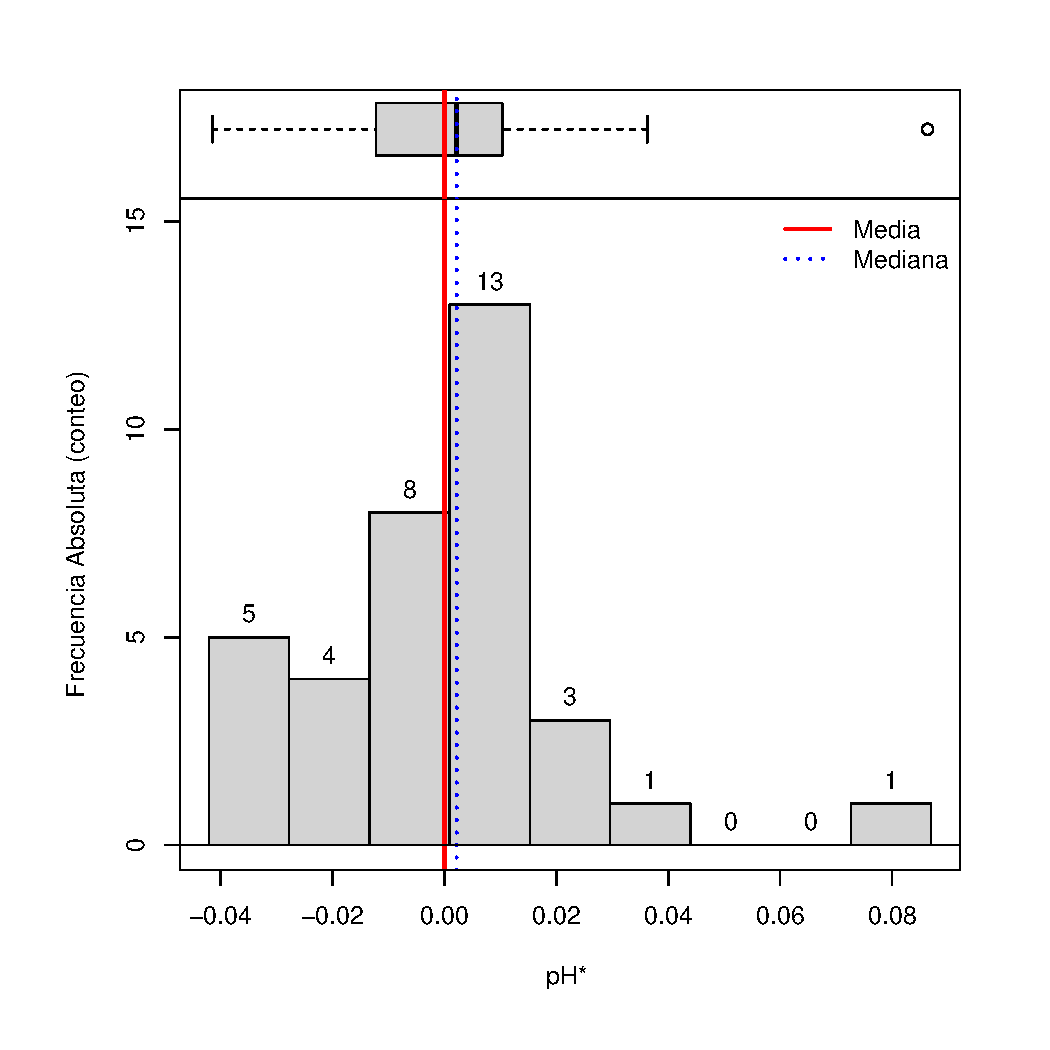
\includegraphics[width=0.75\linewidth]{Figuras_AED/VARIOGRAFICO/pH-pH+_HistBoxPlot1.pdf}
    \caption{Histograma y Boxplot de la diferencia (Z-Z*) del parámetro pH}
    \label{fig:enter-label232}
\end{figure}


La Figura \ref{fig:enter-label232} muestra la distribución de los residuos de la validación cruzada del pH mediante un histograma y un boxplot superpuesto. El histograma indica que la mayoría de las diferencias (pH*) se concentran alrededor de cero, sugiriendo que las estimaciones del modelo están cerca de los valores observados. Las líneas verticales, media (línea roja sólida) y mediana (línea azul punteada), indican un pequeño sesgo a la derecha del cero y una mediana en cero, respectivamente, sugiriendo una estimación sin sesgo significativo. El boxplot revela la dispersión y simetría de los residuos, con un rango intercuartílico (RIQ) que muestra la mitad central de los datos y "bigotes" representando el rango total, excluyendo los outliers marcados por círculos. La mediana centrada y la proximidad entre la media y la mediana sugieren una distribución simétrica de las diferencias. La concentración de la mayoría de las diferencias cerca de cero indica una estimación precisa del pH, aunque la presencia de outliers justifica una investigación adicional para entender las discrepancias.



 \begin{comment}
     

\begin{figure}[!htb]
    \centering
    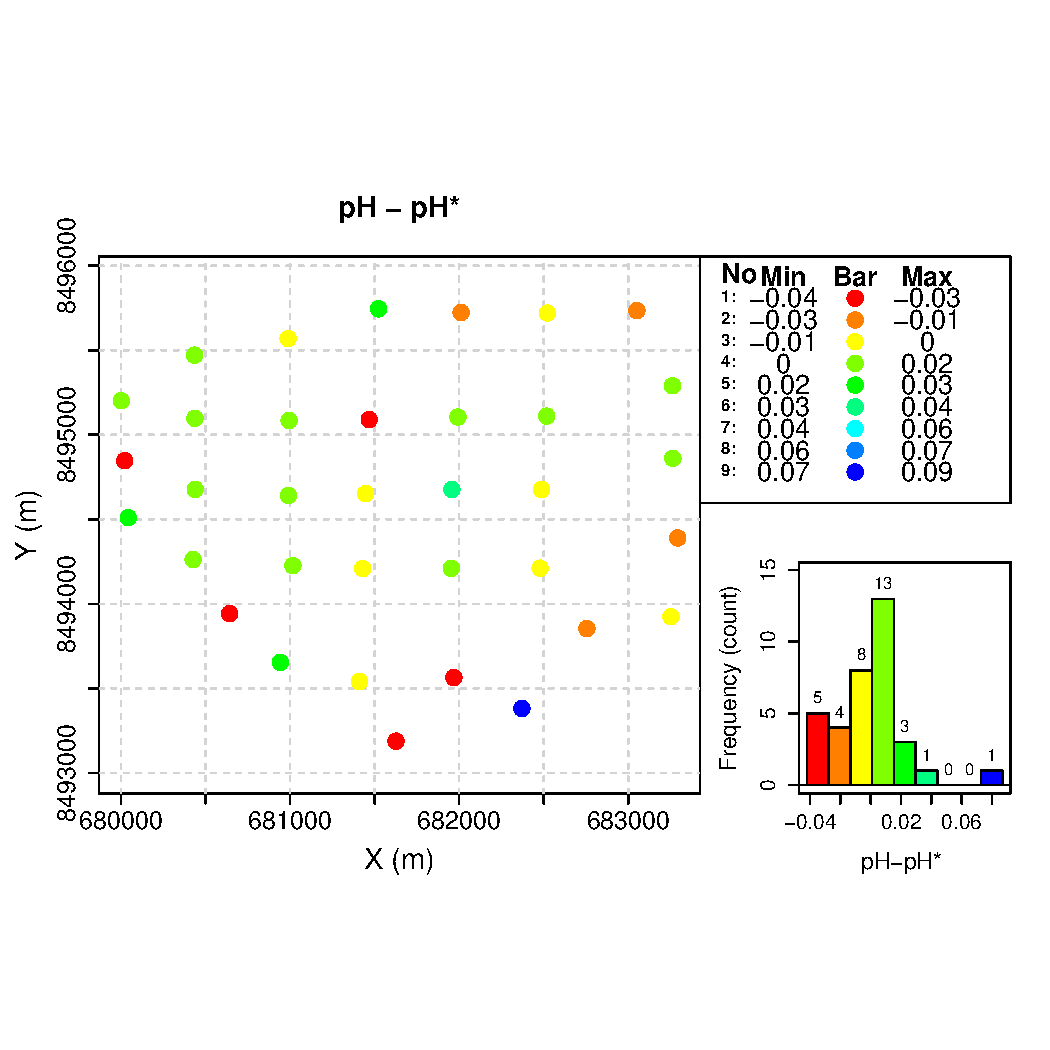
\includegraphics[width=0.9\linewidth]{Figuras_AED/VARIOGRAFICO/pH_CrossValid_Spatial_Distr.pdf}
    \caption{ Distribución espacial de las diferencias (Z-Z*) para el pH}
    \label{fig:enter-label3er}
\end{figure}

La Figura \ref{fig:enter-label3er}   ilustra la distribución espacial de las diferencias entre los valores observados y estimados de pH (\(pH - pH^*\)) en coordenadas geoespaciales. Los puntos están codificados por colores en función de su rango de diferencia, proporcionando una visualización directa de las áreas con mayores discrepancias entre las mediciones y las predicciones del modelo. Aunque algunos puntos, especialmente aquellos codificados con colores que representan los extremos de la escala, pueden parecer outliers, es importante considerar su ubicación espacial antes de llegar a tal conclusión. Estos puntos se encuentran en los extremos del área muestreada y, por lo tanto, su naturaleza de outlier no puede ser confirmada sin ambigüedad. Esto se debe a que los valores atípicos en los bordes del dominio estudiado pueden ser simplemente el resultado de variaciones naturales en el pH o de una menor densidad de datos que no permite una estimación robusta del modelo en estas regiones periféricas. El histograma insertado en la esquina inferior derecha proporciona una visión general de la frecuencia de las diferencias, donde la mayoría de los valores se agrupan alrededor de cero, indicando un buen ajuste general del modelo a los datos.

 \end{comment}

 
\section{Estimación con Kriging Ordinario}
\subsection{Kriging para la Temperatura}

\begin{figure}[!htb]
    \centering
    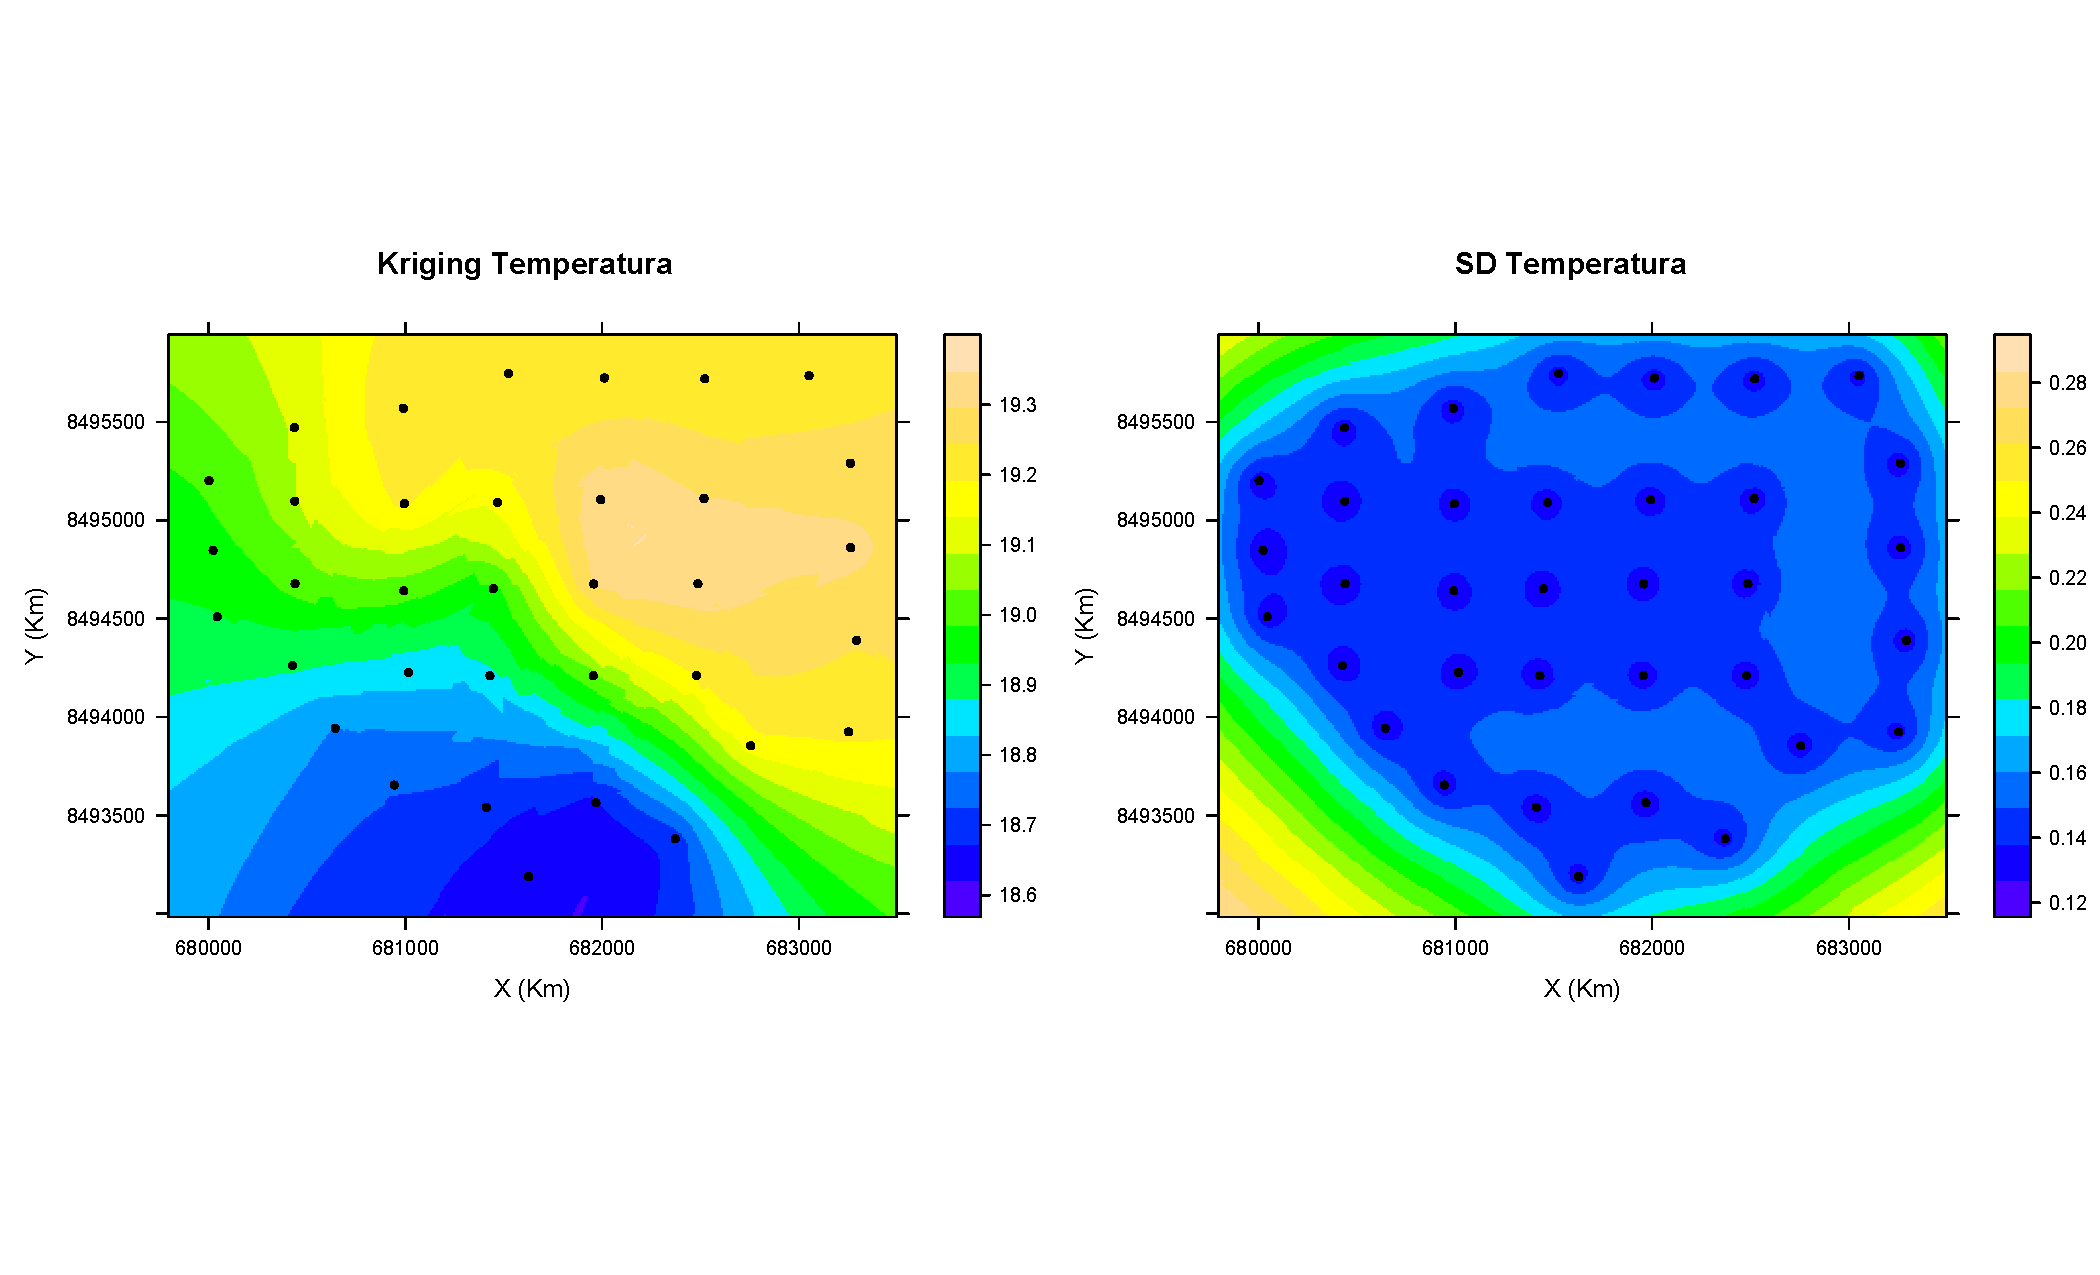
\includegraphics[width=1\linewidth]{Figuras_AED/ESTIMACION/Temperatura_KRIGING.pdf}
    \caption{Mapeo Kriging de Temperatura y Análisis de Incertidumbre}
    \label{fig:enter-labelest}
\end{figure}

En la Figura \ref{fig:enter-labelest}, se presentan los resultados del análisis de interpolación espacial mediante kriging ordinario para la variable temperatura en la laguna Pacucha, con el objetivo de estimar parámetros fisicoquímicos en diferentes áreas. La subfigura (a) muestra la distribución espacial de la temperatura, destacando un gradiente con valores más altos en la parte superior derecha y más bajos hacia la inferior izquierda, mientras que los círculos blancos indican los puntos de muestreo. La subfigura (b) representa la desviación estándar de las estimaciones de kriging, con colores más oscuros sugiriendo mayor confianza y colores más claros mayor incertidumbre en las predicciones. Estos resultados proporcionan una comprensión detallada de la variabilidad espacial de la temperatura, crucial para la gestión de recursos naturales y la planificación ambiental. La técnica de kriging ordinario fue seleccionada por su eficacia en predecir valores en ubicaciones no muestreadas, basándose en la estructura de autocorrelación espacial de los datos.


\subsection{Kriging para el Oxigeno Disuelto}
\begin{figure}[!htb]
    \centering
    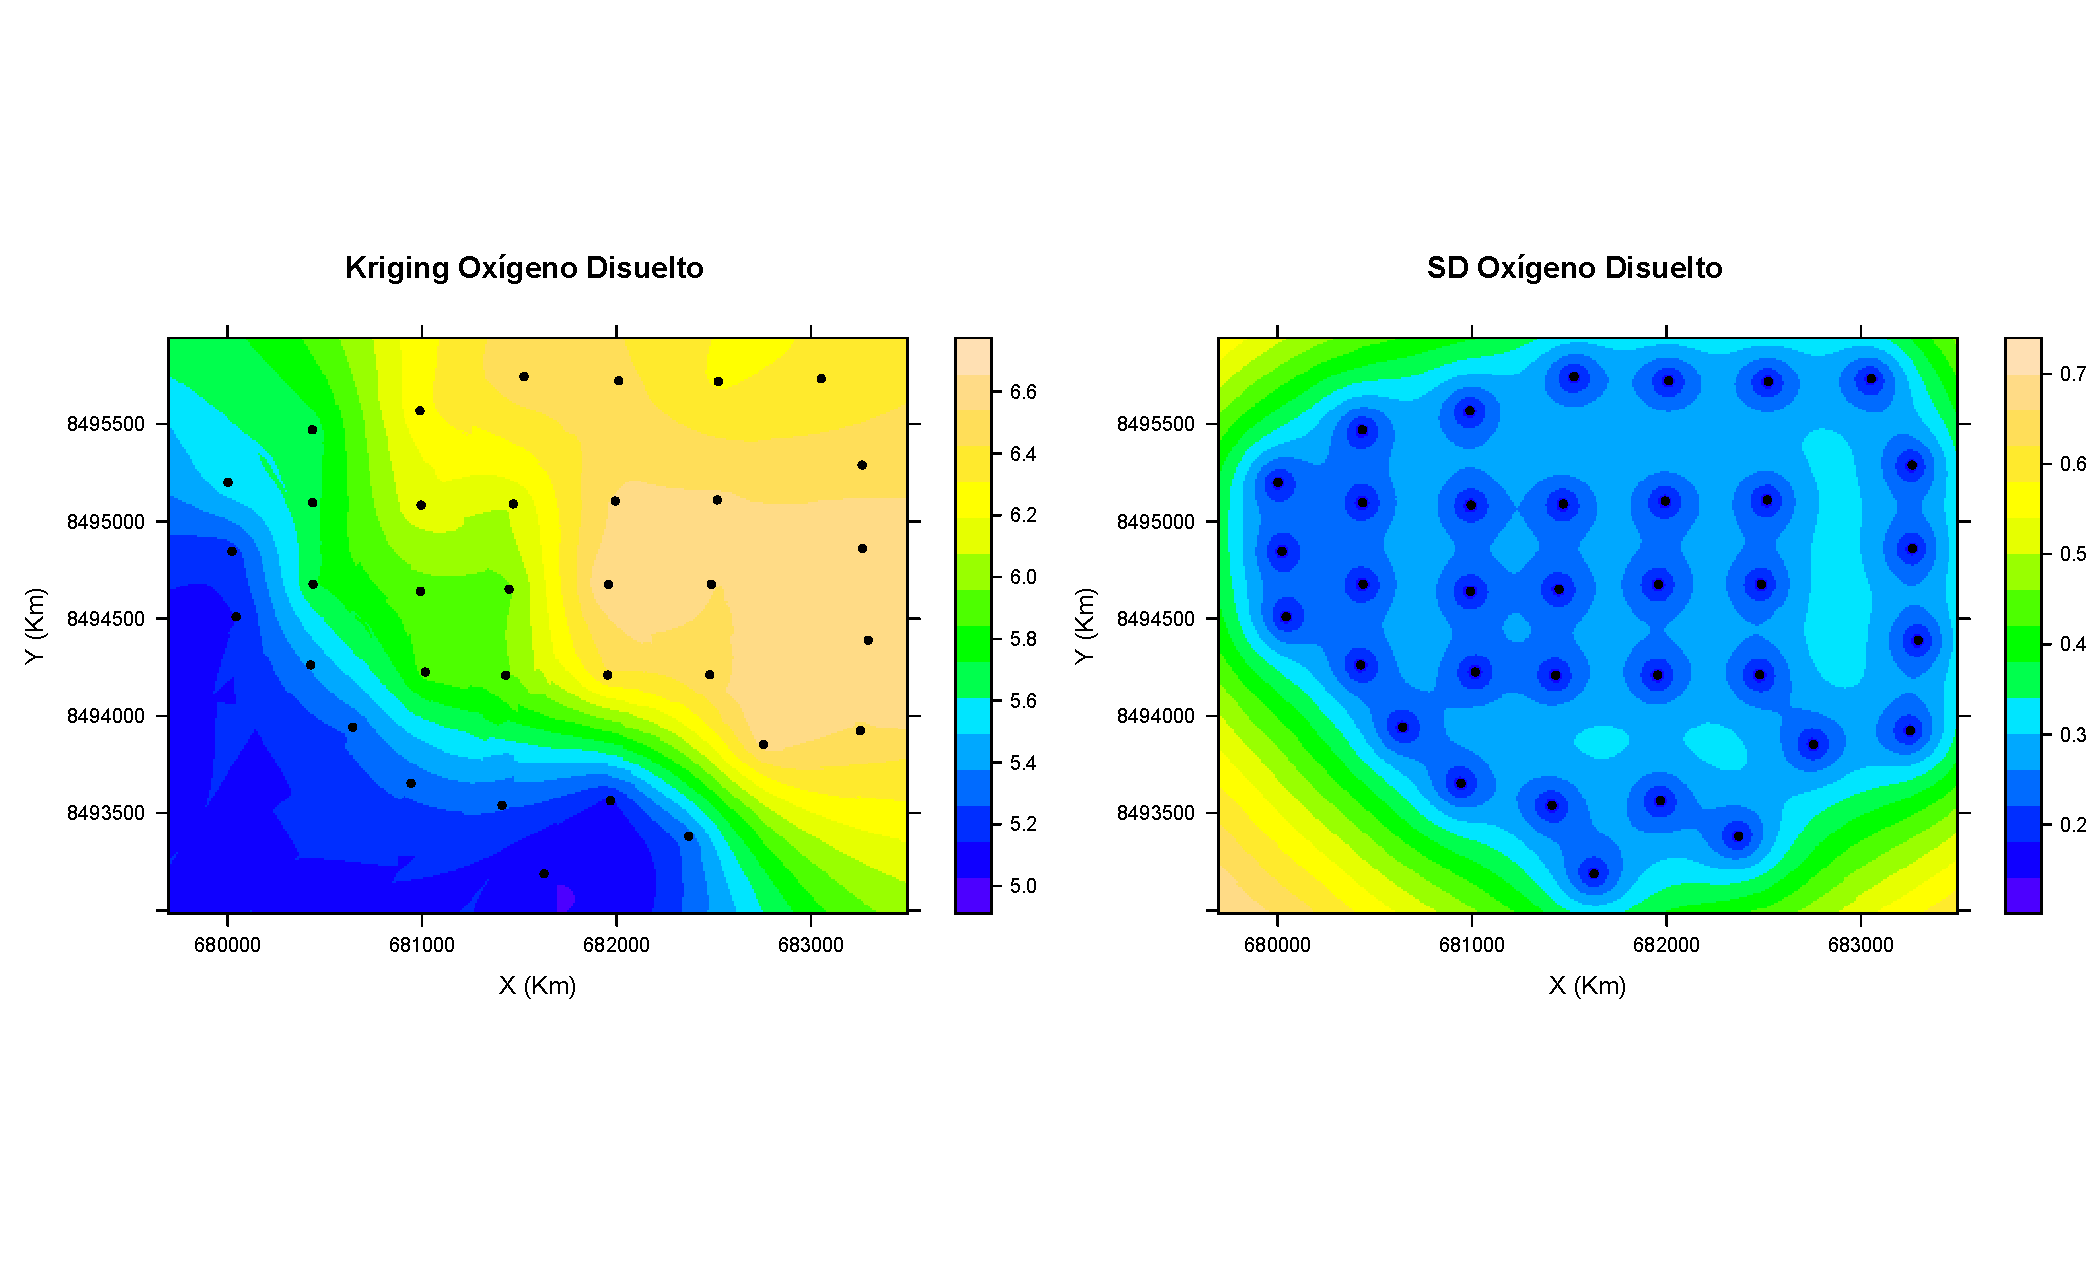
\includegraphics[width=1\linewidth]{Figuras_AED/ESTIMACION/OD_KRIGING.pdf}
    \caption{Mapeo Kriging del Oxigeno Disuelto y Análisis de Incertidumbre}
    \label{fig:enter-labelcdf}
\end{figure}

 La Figura \ref{fig:enter-labelcdf} muestra los resultados del kriging ordinario aplicado a una región acuática específica, explotando la correlación espacial de las muestras (círculos blancos) para predecir valores en ubicaciones no medidas con alta precisión. Utilizando un modelo de variograma esférico ajustado a la semivarianza empírica, se logró un buen ajuste. La imagen (a) representa la concentración estimada de oxígeno disuelto, con un gradiente de colores que refleja variaciones espaciales. La imagen (b) muestra la desviación estándar de las estimaciones, destacando áreas de mayor y menor fiabilidad. Esta técnica es crucial para la gestión de la calidad del agua y la conservación de hábitats acuáticos, permitiendo identificar zonas críticas y planificar futuros muestreos en áreas con mayor incertidumbre.


\subsection{Kriging para el pH}
\begin{figure}[!htb]
    \centering
    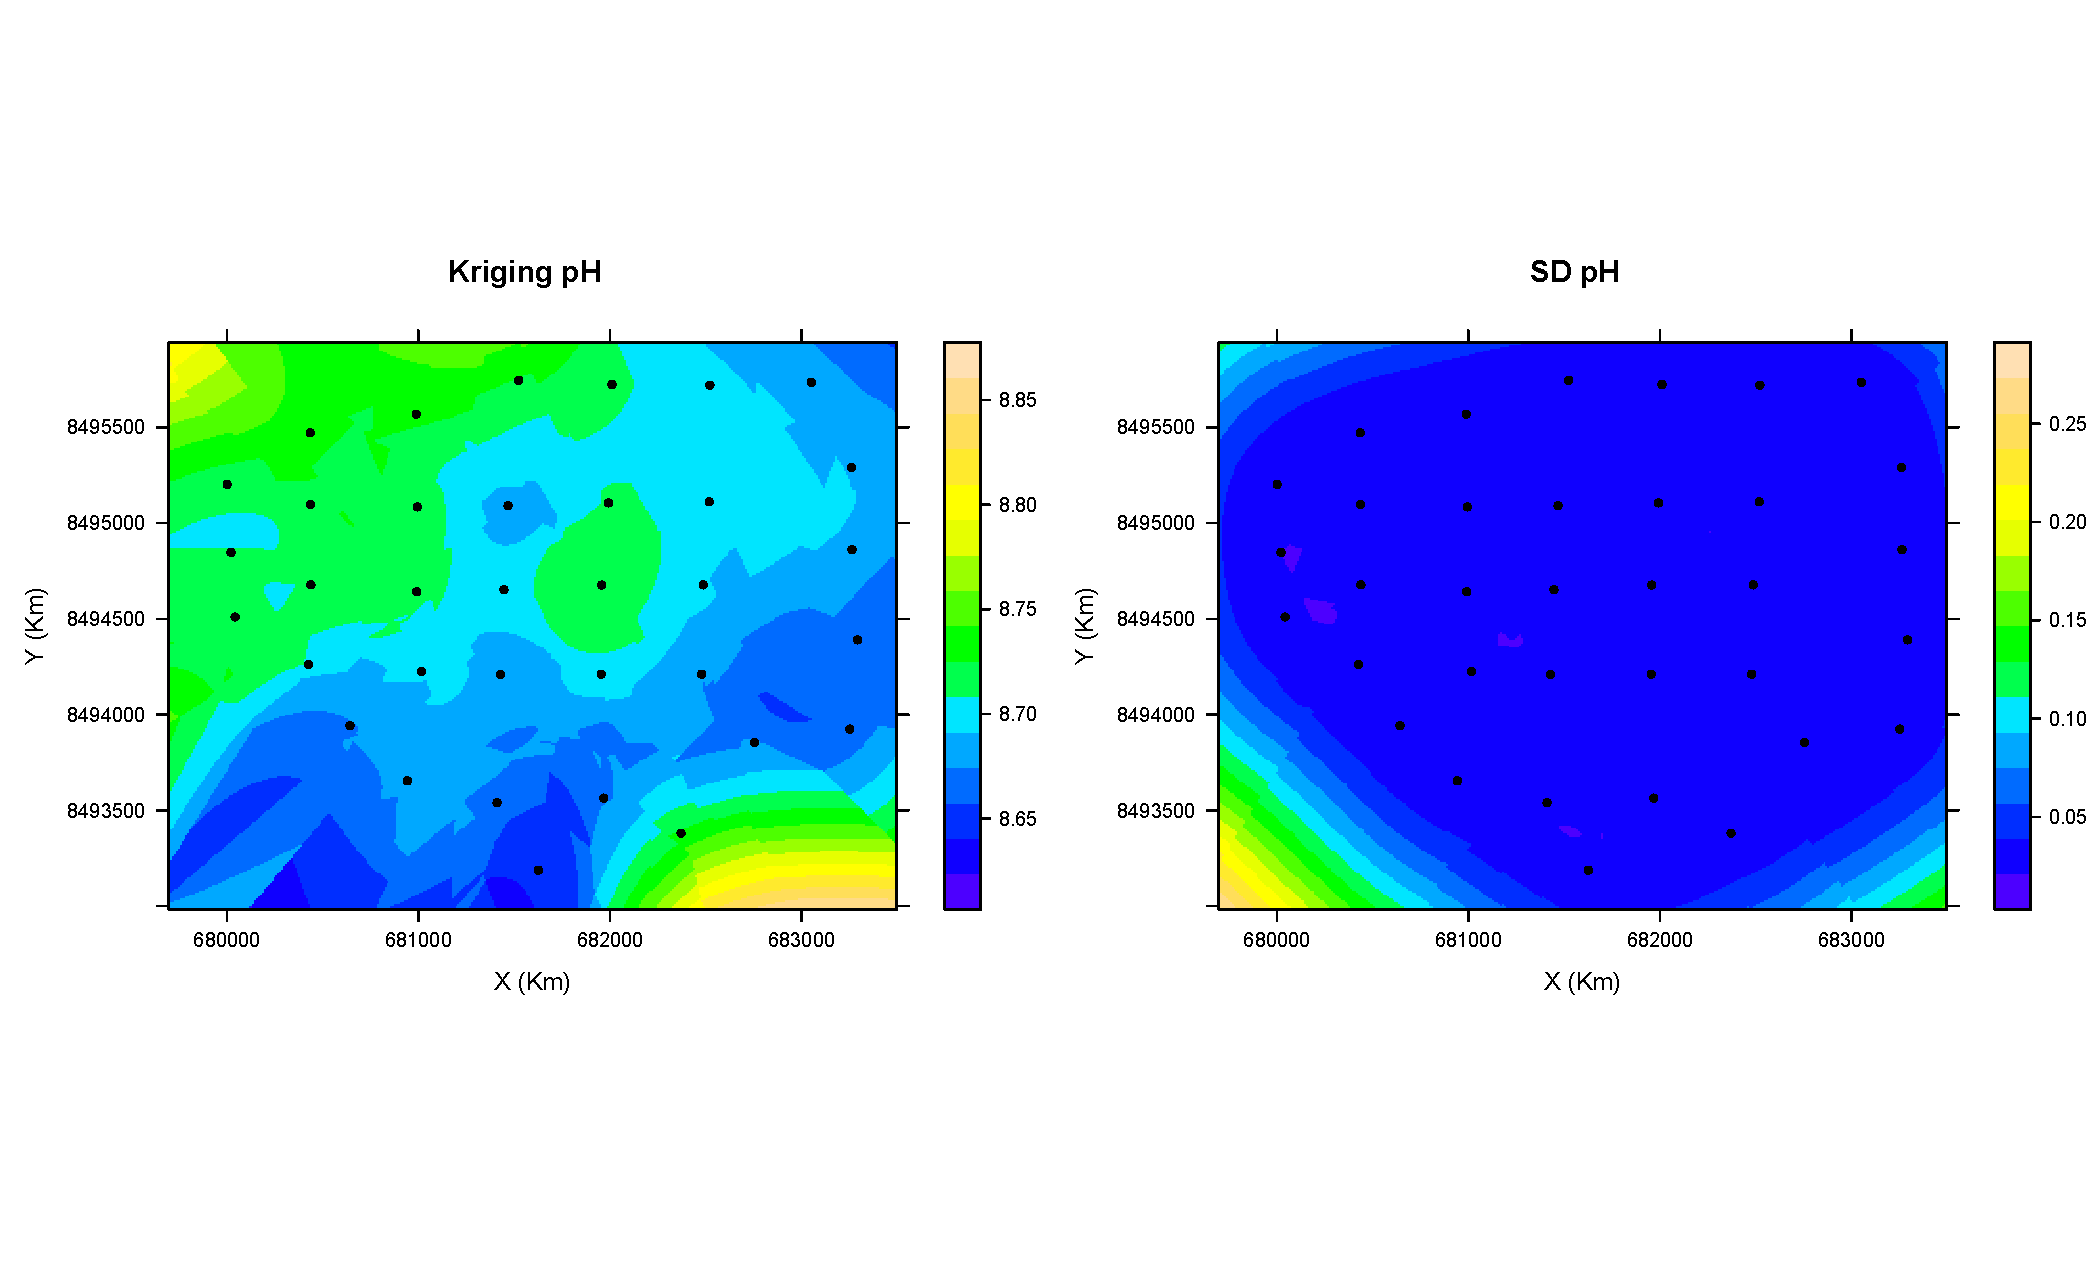
\includegraphics[width=0.9\linewidth]{Figuras_AED/ESTIMACION/PH_KRIGING.pdf}
    \caption{Mapeo Kriging del pH y Análisis de Incertidumbre }
    \label{fig:enter- kring_t55}
\end{figure}

 La Laguna de Pacucha ha sido cartografiada por La Gráfica \ref{fig:enter- kring_t55} utilizando dos mapas de contorno que representan estimaciones del pH utilizando el modelo de kriging gaussiano. El mapa de la izquierda, titulado "Kriging pH", muestra la distribución espacial del pH en la laguna, con una paleta de colores que va del azul (que indica valores de pH más bajos) al amarillo (que indica valores de pH más altos). Los puntos negros representan los lugares donde se realizaron las mediciones del pH. Este mapa de contorno revela un importante gradiente de pH a través del lago, con zonas centrales de alta alcalinidad y regiones más ácidas hacia los bordes.

El mapa de la derecha, titulado "SD pH", ilustra la variabilidad espacial de las estimaciones de pH a través de la desviación estándar de los valores estimados. Los colores más oscuros representan una menor variabilidad, mientras que los colores más claros y los más cercanos al amarillo indican una mayor incertidumbre en las estimaciones. Este mapa es crucial para comprender la fiabilidad de las estimaciones de kriging, ya que muestra que la mayor variabilidad se encuentra en las zonas periféricas del lago, lo que podría indicar una menor densidad de puntos de muestreo o transiciones más bruscas en la composición química del lago. En conjunto, estos mapas proporcionan una visión completa de la distribución del pH en el lago Pacucha y destacan las áreas donde se requiere una investigación más detallada debido a la alta variabilidad de las estimaciones.

\section{ Modelo de corregionalización lineal entre oxígeno disuelto y temperatura }

\subsection{Estimación del variograma experimental}
\begin{figure}[!htb]
    \centering
    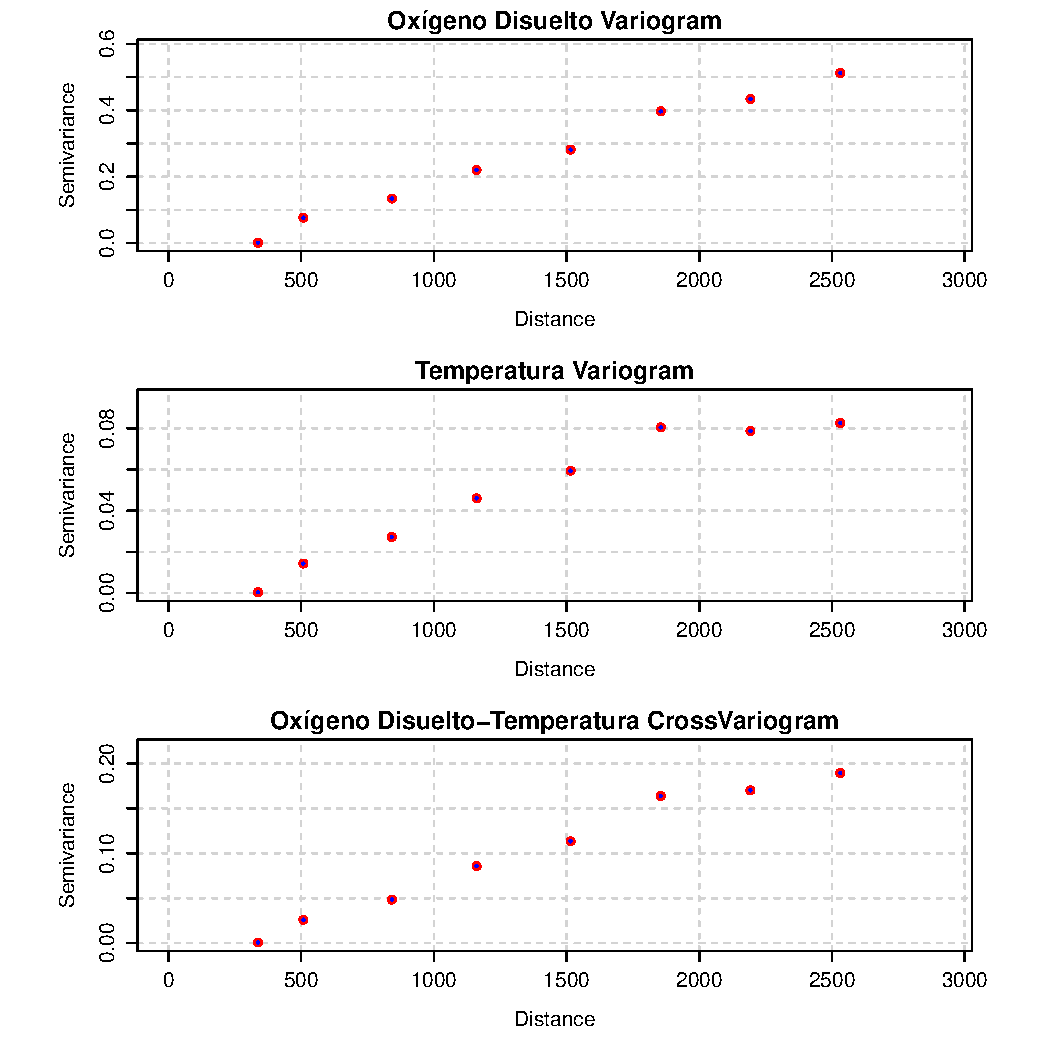
\includegraphics[width=1\linewidth]{Figuras_AED/ESTIMACION/tem_od_CrossVario.pdf}
    \caption{Variograma cruzado entre Oxigeno Disuelto y Temperatura}
    \label{fig:enter-label1235}
\end{figure}


La Figura \ref{fig:enter-label1235} muestra tres variogramas: el del oxígeno disuelto indica un incremento de semivarianza con la distancia, reflejando una mayor disimilitud entre muestras más distantes; el de temperatura también muestra un aumento de semivarianza sin un patrón claro de estabilización, sugiriendo una estructura compleja de correlación o un rango de autocorrelación no alcanzado; y el variograma cruzado entre oxígeno disuelto y temperatura presenta una semivarianza cruzada menor que en los variogramas individuales, lo cual podría señalar una correlación cruzada decreciente con la distancia, siendo una herramienta útil para analizar cómo covarían estas dos variables en el espacio.


\begin{figure}[!htb]
    \centering
    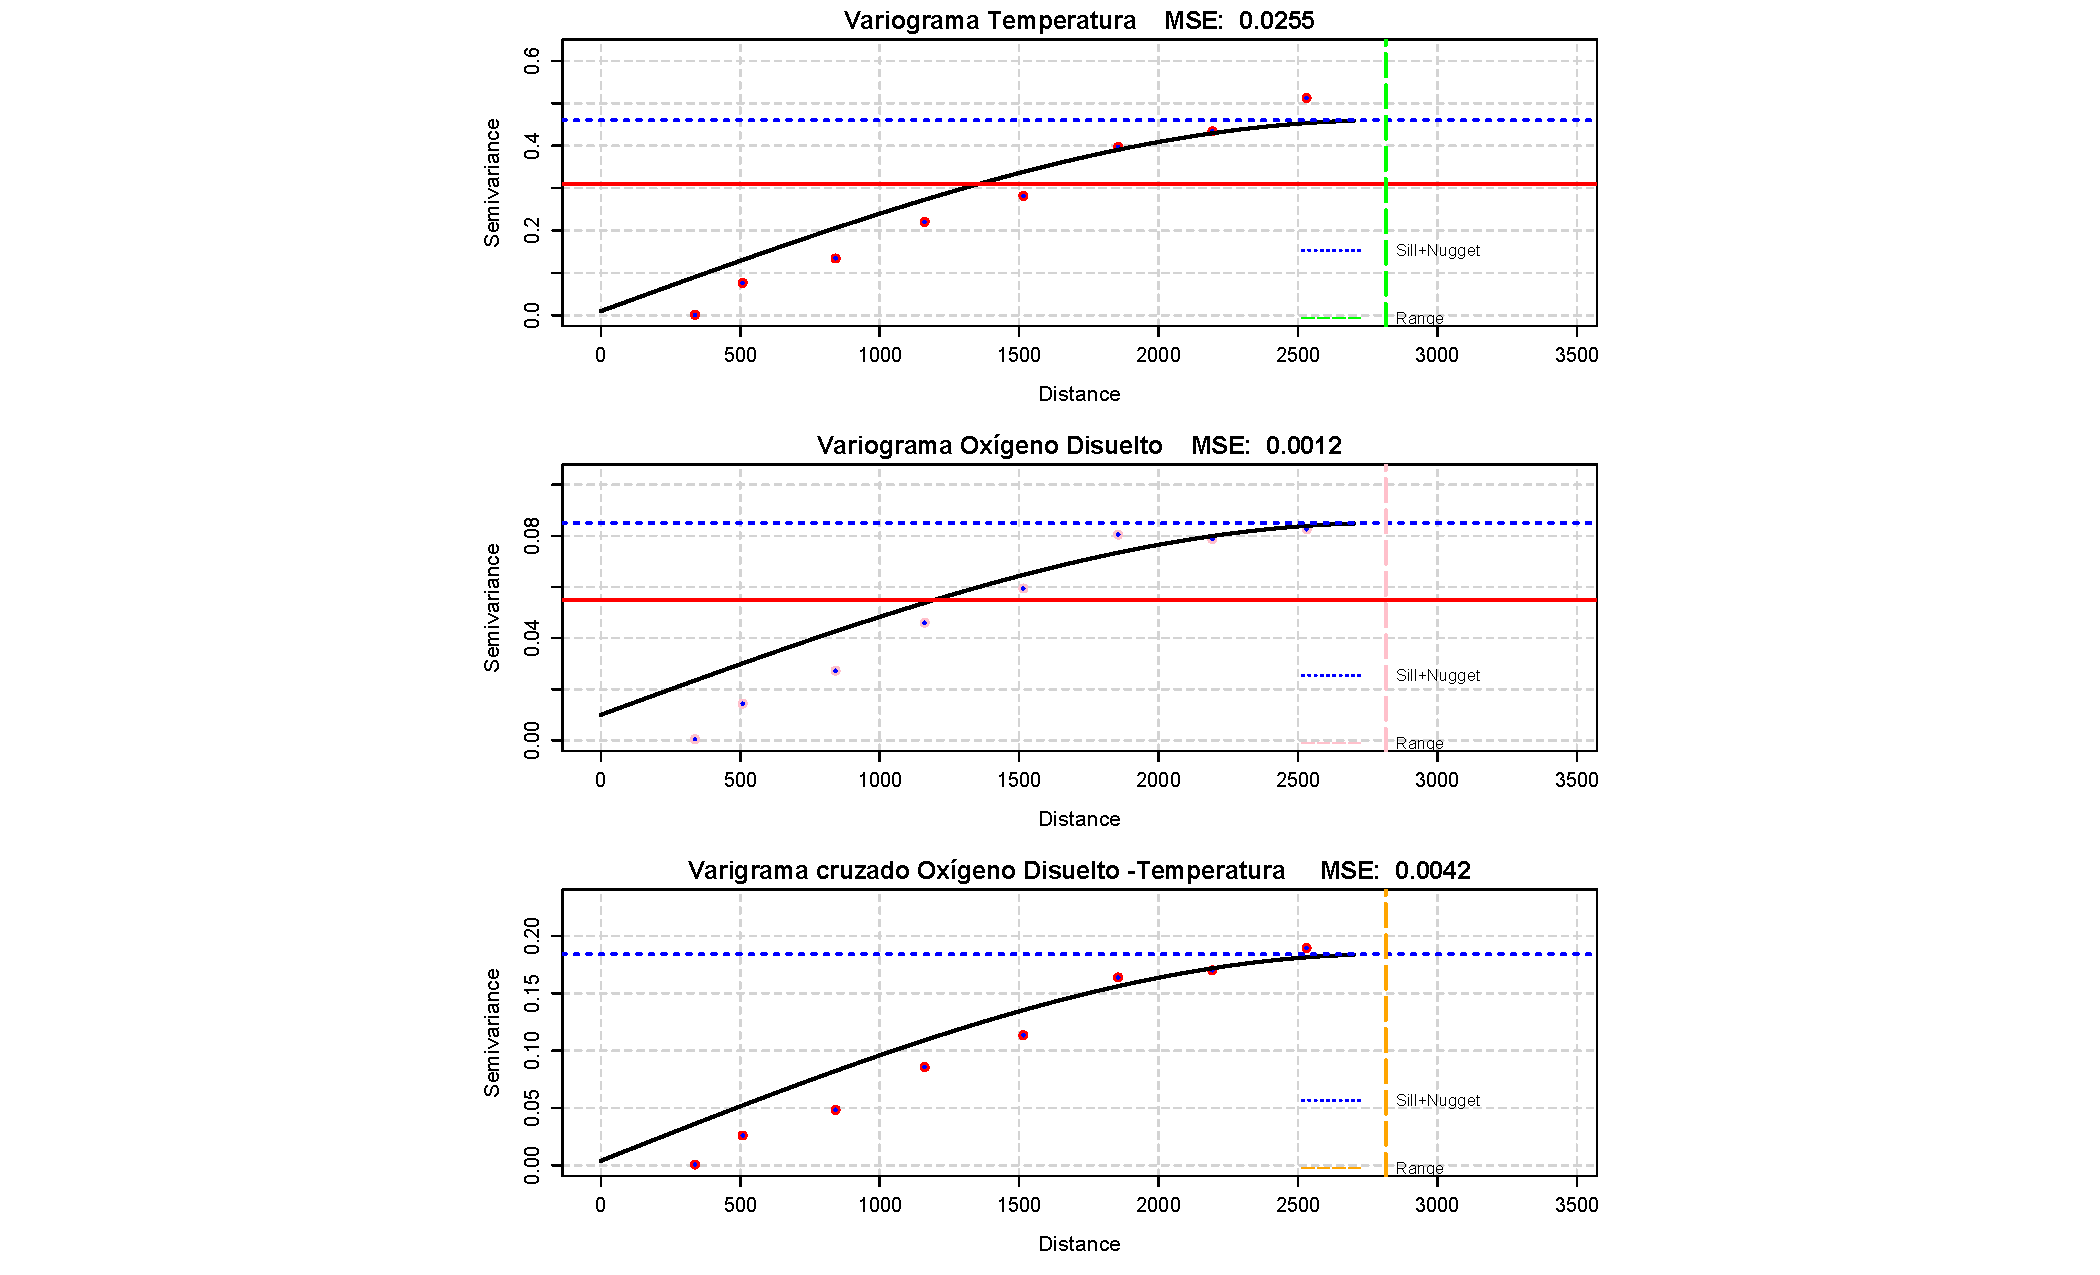
\includegraphics[width=1\linewidth]{Figuras_AED/ESTIMACION/cross_vario_pd_tem.pdf}
    \caption{Modelos de variograma cruzado Oxigeno Disuelto -  Temperatura}
    \label{fig:enter-labelCRER}
\end{figure}

 La Figura \ref{fig:enter-labelCRER} muestra los variogramas presentados son herramientas estadísticas que describen la dependencia espacial de las variables ambientales en la Laguna de Pacucha. El tercer gráfico, denominado "Variograma Cruzado Oxígeno Disuelto-Temperatura", es particularmente notable ya que muestra la correlación espacial entre dos parámetros cruciales del ecosistema acuático: el oxígeno disuelto y la temperatura del agua. Este variograma cruzado indica cómo cambia la relación entre las dos variables con la distancia. La forma del variograma cruzado sugiere que existe una interacción espacial entre el oxígeno disuelto y la temperatura, que es fundamental para comprender cómo interactúan los procesos biológicos y físicos en la laguna.

El variograma cruzado muestra un patrón que comienza con una pequeña "pepita", indicando una fuerte correlación entre el oxígeno disuelto y la temperatura a distancias cortas. A medida que aumenta la distancia, la semivarianza también aumenta, lo que implica que la correlación entre las variables disminuye. El "rango", donde la semivarianza se estabiliza, da una estimación de la distancia más allá de la cual no hay correlación espacial entre las variables. Un error cuadrático medio (ECM) relativamente bajo (0,0042) indica que el modelo de variograma cruzado se ajusta bien a los datos. Estos resultados son esenciales para comprender la dinámica de la laguna de Pacucha y diseñar estrategias de muestreo y gestión ambiental.

\subsection{ Positividad Definida en Modelos de Covarianza para Oxígeno Disuelto y Temperatura}

\begin{table}[!htb]
\centering
\caption{Parámetros de variograma para las variables Temperatura y Oxígeno Disuelto}
\label{tab:variogram_parameters}
{\small % Esto hará que la fuente de la tabla sea pequeña
\begin{tabularx}{\textwidth}{Xcccccc} % X se utilizará para ajustar la columna
\toprule
Variable & Modelo & Nugget & \makecell{Sill-\\Nugget} & \makecell{Sill+\\Nugget} & Alcance & MSE\\
\midrule
Oxígeno Disuelto & Esférico & 0.01 & 0.4500 & 0.4600 & 2815.2 & 0.0255 \\
Temperatura & Esférico & 0.01 & 0.0750 & 0.0850 & 2815.2 & 0.0012 \\
Temperatura-Oxígeno Disuelto & Esférico & 0.05 & 0.1 & 0.15 & 2815.2 & 0.0130 \\
\bottomrule
\end{tabularx}
}
\end{table}
En el estudio de las correlaciones espaciales entre las variables ambientales, se presta especial atención a la positividad definida de los modelos de covarianza. Presentamos aquí un modelo de correolocalización lineal para las variables Temperatura y Oxígeno Disuelto, definido matricialmente como:

La matriz de covarianza bivariable entre oxígeno disuelto y temperatura se define como:

\[
\begin{pmatrix}
\gamma_{TT}(h) & \gamma_{TO}(h) \\
\gamma_{OT}(h) & \gamma_{OO}(h)
\end{pmatrix} = 
\begin{pmatrix}
0.01 & 0.004 \\
0.004 & 0.01
\end{pmatrix} \gamma_0(h) + 
\begin{pmatrix}
0.0750 & 0.1 \\
0.1 & 0.4500
\end{pmatrix} \gamma_1(h),
\]

donde \(\gamma_0(h)\) representa el modelo del efecto nugget y \(\gamma_1(h)\) corresponde al modelo esférico con un alcance de 2815.2000 metros para ambas variables.

Para verificar la condición de positividad definida del modelo, se calculan los determinantes de las matrices de covarianza componentes. A continuación, se presentan los cálculos detallados:

Para la primera matriz:

\[
\text{det} \begin{pmatrix}
0.01 & 0.004 \\
0.004 & 0.01
\end{pmatrix} = (0.01 \times 0.01) - (0.004 \times 0.004) = 0.0001 - 0.000016 = 0.000084 > 0
\]

Para la segunda matriz:

\[
\text{det} \begin{pmatrix}
0.0750 & 0.1 \\
0.1 & 0.4500
\end{pmatrix} = (0.0750 \times 0.4500) - (0.1 \times 0.1) = 0.03375 - 0.01 = 0.02375 > 0
\]

Los determinantes positivos de estas matrices confirman que el modelo de covarianza es positivamente definido. Esta propiedad es crucial para garantizar la coherencia estadística del modelo y la validez de las estimaciones geoestadísticas. Un modelo de covarianza positivamente definido asegura que las varianzas y covarianzas cumplan con los principios fundamentales de la teoría de la variografía, proporcionando una base matemática sólida para el análisis espacial de las variables oxígeno disuelto y temperatura.

% En resumen, la positividad definida de las matrices de covarianza verifica la robustez y aplicabilidad del modelo propuesto, permitiendo realizar estimaciones precisas y fiables en estudios geoestadísticos. Esto es fundamental para cualquier análisis que busque entender y modelar la variabilidad espacial de parámetros ambientales críticos como el oxígeno disuelto y la temperatura.


\subsection{Validación cruzada del variograma OD-Temperatura}

\begin{longtable}{cccccc}
\caption{Resultados de la validación cruzada del variograma entre el Oxígeno Disuelto y la Temperatura} 
\label{fig:cross}
\\
\toprule
N° & X & Y & Z & Z* & Z-Z* \\
\midrule
\endfirsthead

\multicolumn{6}{c}%
{{\bfseries \tablename\ \thetable{} -- continuación de la página anterior}} \\
\toprule
N° & X & Y & Z & Z* & Z-Z* \\
\midrule
\endhead

\bottomrule
\endfoot
1&  682370.9 &8493381& 5.29 &5.386623 &-0.09662282\\
2 & 681968.2& 8493564 &5.08 &5.397385& -0.31738524\\
3  &681626.5 &8493188 &5.03 &5.089849 &-0.05984946\\
4&  681410.7 &8493540& 5.28 &5.268730 & 0.01126970\\
5 & 680942.6& 8493654& 5.30 &5.329394 &-0.02939371\\
6 & 680642.8 &8493942 &5.27 &5.354674 &-0.08467419\\
7&  680426.7 &8494262 &5.39 &5.432779 &-0.04277925\\
8&  680043.0 &8494509 &5.12 &5.304508 &-0.18450835\\
9 & 680022.2 &8494846 &5.17 &5.397877& -0.22787744\\
10 &680001.5& 8495201 &5.58 &5.337437&  0.24256299\\
11& 680435.0 &8495471 &5.64 &5.855081 &-0.21508115\\
12& 680437.3 &8495097& 5.69 &5.739025 &-0.04902455\\
13 &680438.9 &8494677& 5.74 &5.517947 & 0.22205344\\
14& 680991.1& 8494641 &5.91 &5.939596 &-0.02959576\\
15& 681016.2 &8494226 &5.90& 5.652757 & 0.24724270\\
16& 681429.4 &8494209 &5.92& 5.853789 & 0.06621062\\
17 &681446.3 &8494652& 5.91 &6.018217 &-0.10821691\\
18& 681468.0& 8495090 &6.07 &6.248042 &-0.17804173\\
19& 680994.2& 8495084 &6.18 &6.137644 & 0.04235563\\
20& 680988.5 &8495568& 6.29& 6.195579 & 0.09442112\\
21& 681523.6 &8495745 &6.52 &6.322354 & 0.19764585\\
22 &682011.0 &8495723 &6.45& 6.391998 & 0.05800165\\
23 &682521.8 &8495719 &6.28& 6.369621 &-0.08962076\\
24& 683051.2& 8495734 &6.33& 6.296113&  0.03388733\\
25& 683261.6& 8495290 &6.49& 6.434975 & 0.05502501\\
26 &683263.4 &8494861& 6.62& 6.640881 &-0.02088097\\
27 &683292.6& 8494390 &6.65 &6.537744&  0.11225560\\
28& 683252.4& 8493924 &6.52& 6.540246 &-0.02024562\\
29& 682755.0 &8493854 &6.62& 6.364575 & 0.25542524\\
30 &682478.8 &8494211 &6.51& 6.525321 &-0.01532141\\
31 &682486.6 &8494677 &6.54& 6.753546 &-0.21354633\\
32& 682517.5 &8495110 &6.57& 6.528320&  0.04168035\\
33 &681992.6 &8495105 &6.57 &6.619607 &-0.04960708\\
34& 681957.2& 8494676 &6.69 &6.600015&  0.08998518\\
35& 681954.0  &8494210 &6.43 &6.122820&  0.30717967\\
\end{longtable}

La Tabla \ref{fig:cross} muestra los resultados de una validación cruzada para un modelo geoestadístico que relaciona oxígeno disuelto y temperatura. 'Z' son los valores observados, 'Z*' los predichos por el modelo, y 'Z-Z*' indica la discrepancia entre ellos, midiendo la precisión del modelo. Esta validación es crucial para evaluar la confiabilidad del modelo en diversas ubicaciones, garantizando estimaciones espaciales precisas de parámetros ambientales.

\subsubsection{Análisis Descriptivo de la Validación Cruzada del Variograma Cruzado}

\begin{table}[!htb]
\centering
\caption{Estadísticos Descriptivos para la Validación Cruzada del Variograma}
\label{od_tem}
\begin{tabular}{lccc}
\toprule
Estadístico & Z & Z* & Z-Z* \\
\midrule
No. de Muestras & 35.00000 & 35.00000 & 35.00000 \\
Mínimo & 5.03000 & 5.08985 & -0.31739 \\
1er Cuartil & 5.48500 & 5.41533 & -0.08715 \\
Mediana & 6.07000 & 6.12282 & -0.02025 \\
Media & 5.98714 & 5.98586 & 0.00128 \\
3er Cuartil & 6.51500 & 6.41349 & 0.07810 \\
Máximo & 6.69000 & 6.75355 & 0.30718 \\
Rango & 1.66000 & 1.66370 & 0.62456 \\
Rango Intercuartil & 1.03000 & 0.99816 & 0.16525 \\
Varianza & 0.30913 & 0.25978 & 0.02273 \\
Desviación Estándar & 0.55600 & 0.50969 & 0.15075 \\
Simetría & -0.34761 & -0.20678 & 0.13097 \\
Curtosis & 1.64106 & 1.57275 & 2.58988 \\
\bottomrule
\end{tabular}
\end{table}

Los estadísticos descriptivos en la Tabla \ref{od_tem} resumen la validación cruzada del modelo geoestadístico para oxígeno disuelto y temperatura. La tabla incluye media, mediana, rango, desviación estándar, simetría y curtosis para los valores observados (Z), predichos (Z*) y sus diferencias (Z-Z*). La similitud entre medias y medianas indica un buen ajuste del modelo. Los valores positivos en el rango intercuartílico y curtosis para las diferencias sugieren una variabilidad moderada y picos pronunciados en los errores. Estos resultados confirman la eficacia del modelo en capturar la variabilidad espacial de las variables.

\subsubsection{ Histogramas y Diagramas de Caja de las Discrepancias en la Validación Cruzada}

\begin{figure}[!htb]
    \centering
    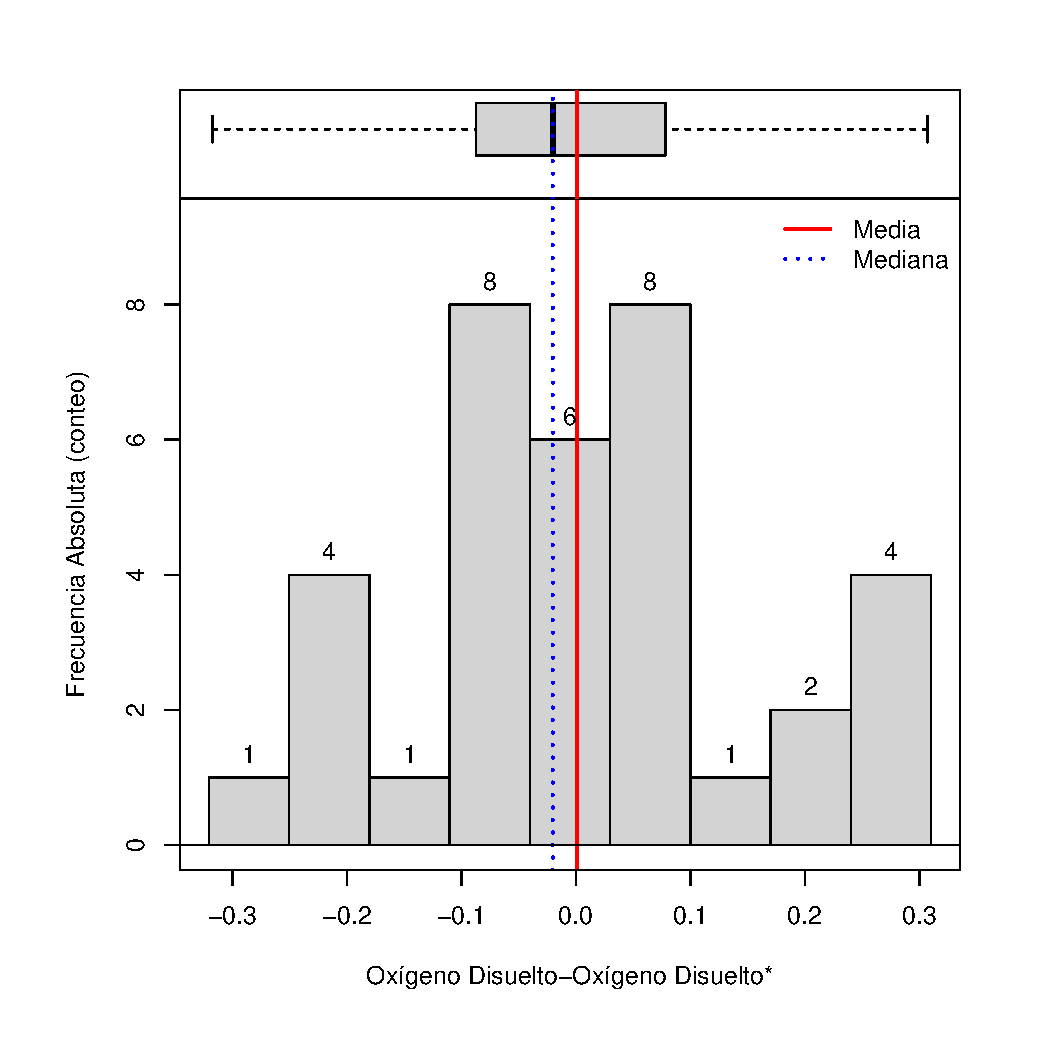
\includegraphics[width=0.5\linewidth]{Figuras_AED//ESTIMACION/Oxígeno_Disuelto-Oxígeno_Disuelt+_HistBoxPlot1CoKrig.pdf}
    \caption{Histogramas y Diagramas de Caja de las (Z-Z*) }
    \label{fig:enter-labelcdfr}
\end{figure}
La Figura  \ref{fig:enter-labelcdfr} enfoca la validación cruzada para la diferencia entre el oxígeno disuelto y la temperatura muestra una distribución de errores centrada cerca de cero, con una media y una mediana visualmente próximas a esta marca, lo que indica un sesgo bajo en las predicciones del modelo. Numéricamente, la mediana de las diferencias está muy próxima a cero, lo que pone de relieve la precisión del modelo, mientras que la media ligeramente desplazada sugiere la influencia de algunos valores atípicos. La frecuencia de los errores se distribuye de forma relativamente uniforme a ambos lados del cero, con un recuento de errores que varía de 1 a 8 para los distintos intervalos, lo que refleja una dispersión moderada de las predicciones en torno a los valores observados. Esto indica un modelo bien ajustado con una variabilidad razonable en las estimaciones.


\begin{comment}
  
\subsubsection{Distribución espacial de las diferencias (Z-Z*)}

\begin{figure}[!htb]
    \centering
    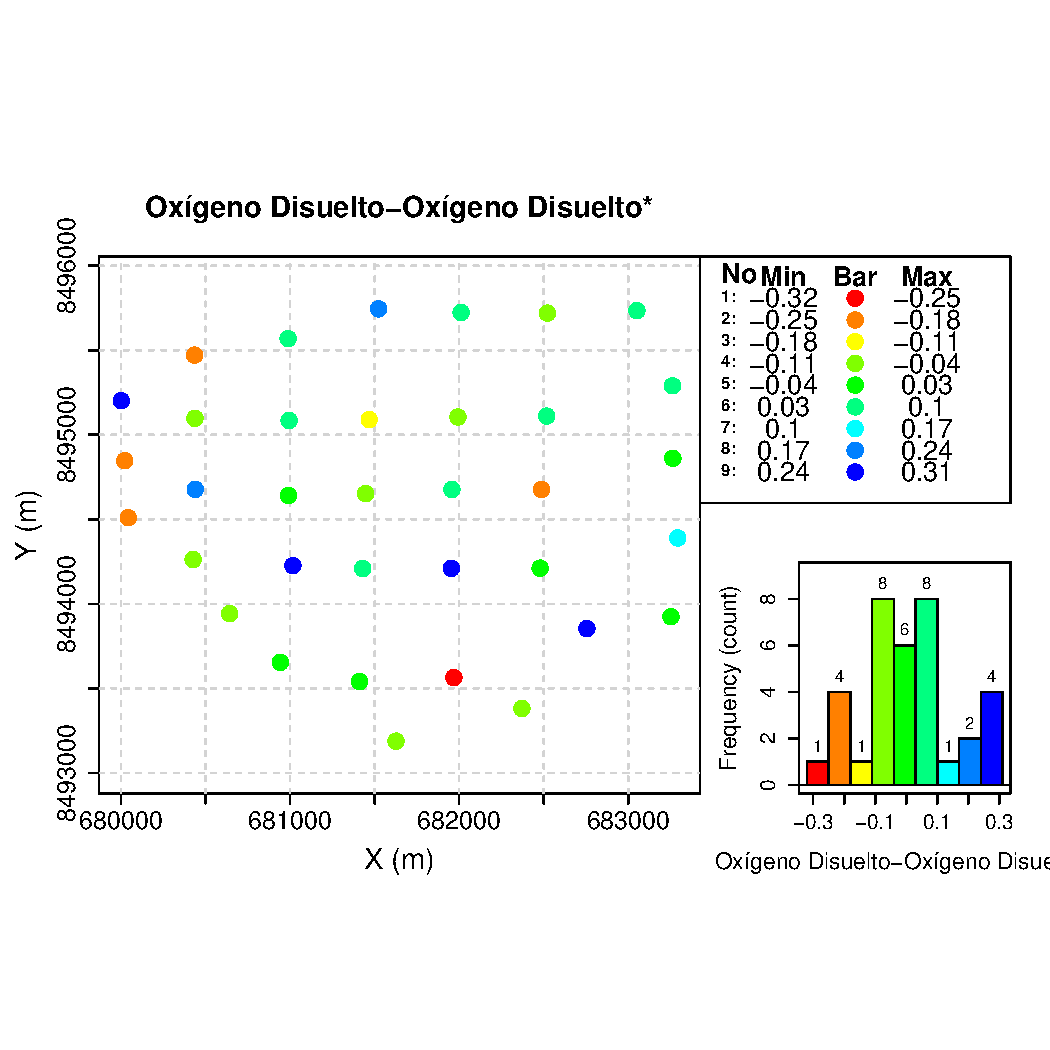
\includegraphics[width=0.8\linewidth]{Figuras_AED/ESTIMACION/OXIGENO_CoKrigingCrossValid_Spatial_Distr.pdf}
    \caption{Distribución espacial de las diferencias de  la estimación de Cokriging Oxigeno disuelto }
    \label{fig:enter-label}
\end{figure}
  
\end{comment}


\section{Co-estimación para la Predicción Espacial de Oxígeno Disuelto en Función de la Temperatura}

\begin{figure}
    \centering
    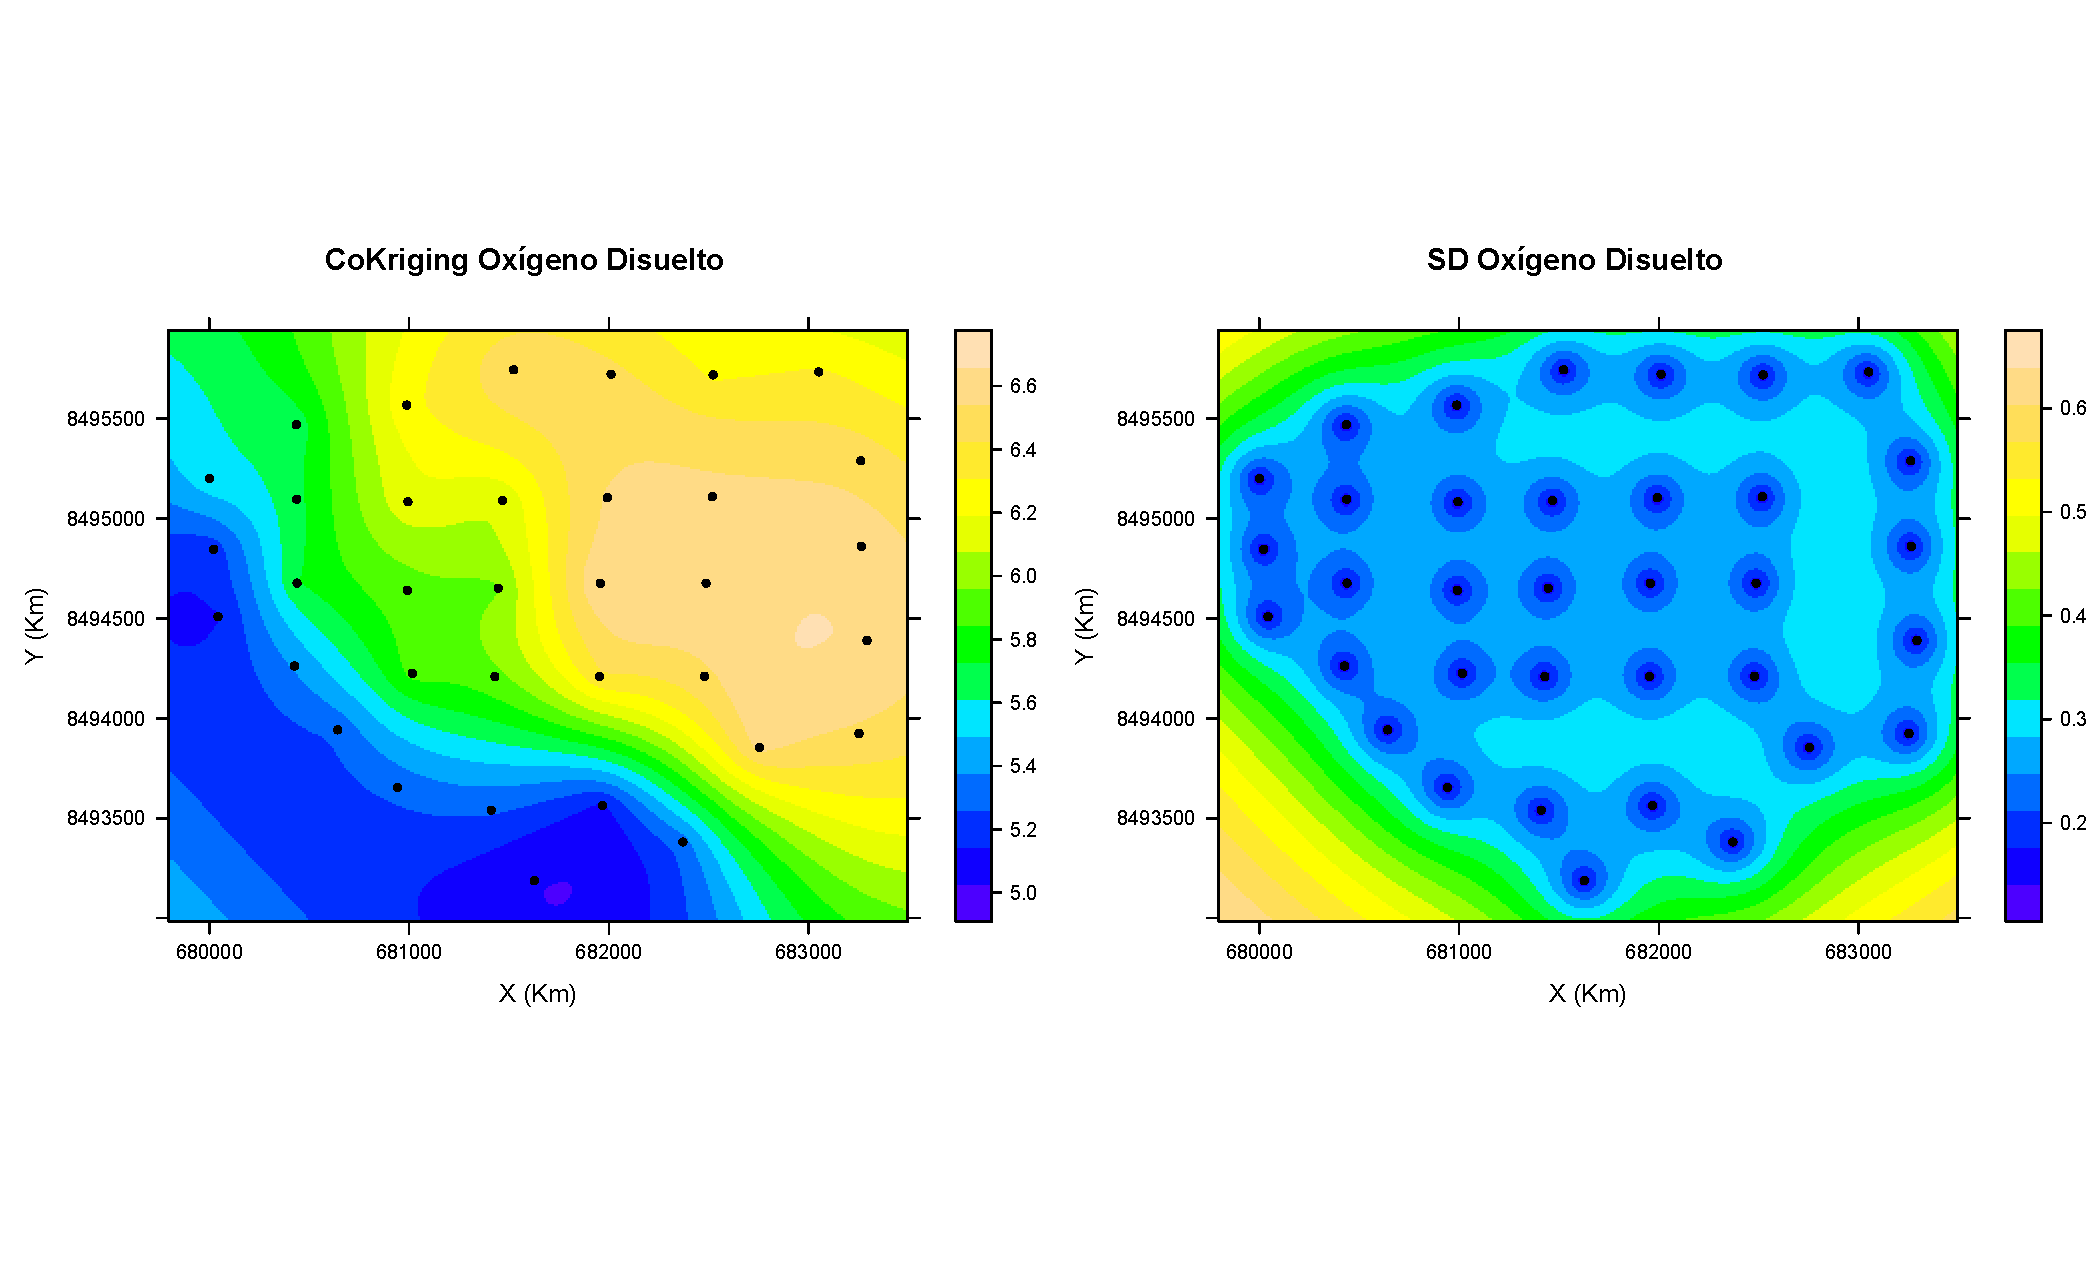
\includegraphics[width=1\linewidth]{Figuras_AED//ESTIMACION/COKRIGING_OD_TEM.pdf}
    \caption{Interpolación espacial y el análisis de incertidumbre en la estimación de oxígeno disuelto mediante cokriging en relación a la temperatura en la Laguna de Pacucha}
    \label{fig:enter-cokrigong}
\end{figure}


La Figura \ref{fig:enter-cokrigong} presenta dos mapas de interpolación geoestadística de la distribución espacial del oxígeno disuelto en la Laguna de Pacucha, calculada mediante la técnica de cokriging basada en la temperatura del agua. 

El mapa de la izquierda, titulado ``Cokriging Oxígeno Disuelto'', muestra los niveles de oxígeno disuelto con una escala de colores que varía del azul (menor concentración) al amarillo (mayor concentración), y los puntos negros indican las ubicaciones de las mediciones in situ utilizadas para generar la interpolación.

El mapa de la derecha, denominado ``SD Oxígeno Disuelto'', ilustra la desviación estándar de las estimaciones de cokriging, con tonalidades más oscuras indicando mayor incertidumbre y áreas claras reflejando mayor confianza en las estimaciones. Este análisis de incertidumbre es fundamental para evaluar la confiabilidad de los datos interpolados y dirigir futuros esfuerzos de muestreo hacia las áreas que requieren mayor precisión en las mediciones.


\subsection{ Evaluación Comparativa entre Kriging y Cokriging para la Estimación del Oxígeno Disuelto
}


\begin{figure}[h]
    \centering
    \includegraphics[width=0.45\textwidth]{Figuras_AED/ESTIMACION/KrigingOD.png} 
     %\hfill Este comando inserta un espacio que se ajustará automáticamente para que las imágenes se separen horizontalmente
    \includegraphics[width=0.45\textwidth]{Figuras_AED/ESTIMACION/CoKriging_od.png} % Reemplace con el nombre de su archivo de imagen
    \caption{Comparación entre los métodos de Kriging y Cokriging para la estimación del oxígeno disuelto en la Laguna de Pacucha.}
    \label{fig:kriging_cokrigingza1}
\end{figure}
  
  Al evaluar las técnicas de Kriging y Cokriging para estimar el oxígeno disuelto en el lago Pacucha Figura \ref{fig:kriging_cokrigingza1}, observamos que ambos métodos proporcionan una visualización detallada de la variabilidad espacial de este parámetro esencial. El Kriging, método de interpolación que utiliza únicamente información de la variable de interés, en este caso el oxígeno disuelto, muestra una distribución que indica claros gradientes de concentración a lo largo del lago. Los valores estimados oscilan entre 5,0 mg/L y 6,6 mg/L, lo que indica en general una calidad del agua adecuada para la vida acuática en la mayor parte del lago.

Por otra parte, el Cokriging incorpora información de una o más variables correlacionadas, como la temperatura del agua, para mejorar las estimaciones del parámetro principal. Esta técnica puede proporcionar estimaciones más precisas en lugares donde las mediciones directas son escasas, aprovechando la relación entre parámetros. En la imagen de Cokriging, vemos que la variabilidad espacial del oxígeno disuelto sigue un patrón similar al presentado en el mapa de Kriging, lo que puede ser indicativo de una fuerte correlación entre el oxígeno disuelto y las variables auxiliares utilizadas en el análisis.


\section{Evaluación de la Calidad del Agua en la Laguna de Pacucha}

\subsection{Comparación con los Estándares de Calidad Ambiental}

\begin{comment}
    La integridad ecológica de ambientes acuáticos como la Laguna de Pacucha es crucial para preservar la diversidad biológica y asegurar la funcionalidad del ecosistema. En este contexto, los criterios establecidos por el Decreto Supremo N° 004-2017-MINAM de Perú proporcionan un marco para evaluar la calidad del agua, centrándose en indicadores clave como el oxígeno disuelto, el pH y la temperatura. Estos parámetros, centrales en el presente estudio, no solo reflejan la salud del ecosistema acuático, sino que son vitales para la supervivencia de las especies que lo habitan. Además, se destaca la importancia de la geoestadística como metodología avanzada para investigar la calidad ambiental de los recursos hídricos, lo que permite una interpretación más precisa y espacialmente integrada de los datos.

\section{Evaluación de Oxígeno Disuelto}
 El oxígeno disuelto (OD) es un parámetro fundamental para evaluar la calidad del agua y su capacidad para sustentar la vida acuática. Según el Decreto Supremo N° 004-2017-MINAM en el Perú, el umbral mínimo aceptable de OD fue de 4 mg/L. La aplicación de técnicas geoestadísticas, como Kriging, revela que en la laguna Pacucha los niveles de OD fluctúan entre 5,00 mg/L y 6,60 mg/L. Estos valores sugieren que amplias zonas de la laguna mantienen una calidad de agua propicia para el florecimiento de la biota acuática. Sin embargo, hay zonas en las que el OD se acerca al límite inferior, con lecturas de 5,00 mg/L, lo que hace temer una posible tendencia a la baja que podría poner a la laguna en riesgo de caer por debajo del umbral crítico de 4,0 mg/L con el tiempo.

Este límite casi inferior es una señal de alarma para la conservación de los ecosistemas lagunares. Puede ser precursor de unas condiciones menos óptimas para la vida acuática, en particular para las especies sensibles, y es un claro indicio de la necesidad de adoptar medidas de gestión. El descenso de los niveles de oxígeno disuelto podría estar relacionado con las actividades humanas en las inmediaciones de la laguna de Pacucha. Las prácticas predominantes en la región, como la agricultura y el turismo, pueden contribuir a este fenómeno. Por lo tanto, es imperativo implementar un monitoreo continuo y estrategias de gestión ambiental para mitigar los impactos humanos y asegurar la preservación de esta valiosa reserva acuática para las generaciones futuras.

\subsection*{Evaluación de pH}
 El pH es un parámetro fundamental en ecología acuática, ya que regula la disponibilidad de nutrientes y metales, y ejerce una influencia significativa en los procesos biológicos de los organismos que habitan en el agua. Según el Decreto Supremo N° 004-2017-MINAM de Perú, el rango de pH considerado óptimo para la mayoría de los ecosistemas acuáticos es de 6.5 a 8.5, lo que garantiza un ambiente propicio para el equilibrio ecológico y la biodiversidad.

En la Laguna de Pacucha, los valores estimados de pH varían entre 8.64 y 8.82, ligeramente por encima del límite superior del rango óptimo. Este aumento en la alcalinidad puede tener diversas implicaciones para el ecosistema. Por un lado, un pH elevado puede influir en la solubilidad y, por tanto, en la toxicidad de ciertos metales, lo que podría tener efectos negativos en la flora y fauna acuáticas. Además, puede afectar adversamente a especies sensibles al pH, alterando la reproducción y la supervivencia de ciertos peces y organismos invertebrados.

La tendencia alcalina observada en la Laguna de Pacucha debe ser motivo de un seguimiento detallado. Aunque los valores no se desvían drásticamente del rango óptimo, es importante considerar la variabilidad diurna y estacional del pH y su interacción con otros factores químicos y biológicos. La gestión sostenible de la laguna debe incluir estrategias para monitorear y, si es necesario, ajustar las condiciones del pH para mantener un ecosistema robusto y resiliente.

\subsection*{Evaluación de Temperatura}
 La temperatura del agua es un indicador clave del entorno, ya que regula las tasas metabólicas de los organismos acuáticos y la solubilidad del oxígeno, lo que es esencial para la supervivencia de la fauna acuática. Aunque no hay un estándar específico de temperatura en la normativa, las variaciones significativas pueden tener efectos directos y profundos en la homeostasis del ecosistema.

En la Laguna de Pacucha, los valores de temperatura estimados oscilan entre 18.6 y 19.4 °C, lo que generalmente es benigno para la mayoría de las especies de agua dulce tropicales y subtropicales. Sin embargo, es importante reconocer que incluso pequeñas fluctuaciones dentro de este rango pueden afectar los ciclos de vida, la reproducción y la distribución de especies endémicas y especializadas.

Por lo tanto, la evaluación de la Laguna de Pacucha sugiere que las condiciones actuales de temperatura parecen adecuadas para mantener un ecosistema acuático saludable. No obstante, se debe mantener una vigilancia constante, ya que los impactos antropogénicos o los cambios climáticos podrían alterar este delicado equilibrio térmico. La implementación de programas de monitoreo a largo plazo permitirá detectar tendencias o cambios repentinos en la temperatura del agua, lo que facilitará la implementación de medidas de gestión ambiental oportunas.
\end{comment}


\subsection*{Temperatura}

\begin{table}[H]
\centering
\caption{Comparación de la temperatura con el Estándar de Calidad Ambiental}
\begin{tabular}{p{0.4\linewidth} p{0.5\linewidth}}
\toprule
Parámetro & Valor Estimado \\
\midrule
Rango de Temperatura & 18.6°C a 19.3°C \\
ECA Relevante & Varía hasta 3°C respecto al promedio mensual multianual \\
Conclusión & Cumple con ECA, adecuada para la vida acuática, aunque indica vulnerabilidad a contaminación debido a la presencia de actividad antropogénica \\
\bottomrule
\end{tabular}
\end{table}


\subsection*{pH}

\begin{table}[H]
\centering
\caption{Comparación del pH  con el Estándar de Calidad Ambiental}
\begin{tabular}{ll}
\toprule
Parámetro & Valor Estimado \\
\midrule
Rango de pH & 8.65 a 8.85 \\
ECA Relevante & Debe estar entre 6.5 y 9.0 \\
Conclusión & Cumple con ECA, no representa riesgo para el ambiente  \\
& pero las variaciones podrían hacer vulnerable por contaminantes  \\
\bottomrule
\end{tabular}
\end{table}

\subsection*{Oxígeno Disuelto}


\begin{table}[H]
\centering
\caption{Comparación del oxígeno disuelto  con los Estándar de Calidad Ambiental }
\begin{tabular}{ll}
\toprule
Parámetro & Valor Estimado \\
\midrule
Rango de Oxígeno Disuelto & 5.0 mg/L a 6.6 mg/L \\
ECA Relevante & Mínimo de 4 mg/L para conservación del ambiente acuático \\
Conclusión & Supera el mínimo necesario según ECA,  \\
& La presencia de variaciones sugiere vulnerabilidad  \\

\bottomrule
\end{tabular}
\end{table}

\subsubsection{Observaciones generales}
Los resultados obtenidos de la estimación mediante técnicas de kriging para temperatura,
pH y oxígeno disuelto en la Laguna de Pacucha están en conformidad con los
ECA establecidos. Esto implica que la calidad del agua se mantiene dentro de los límites
aceptables para su uso recreacional y la conservación de la vida acuática, según los
criterios nacionales vigentes. Estos hallazgos respaldan la idoneidad de la laguna para
actividades recreativas y como hábitat para diversas formas de vida acuática, subrayando
la importancia de continuar con el monitoreo regular para preservar estas condiciones.
La integridad ecológica de ambientes acuáticos como la Laguna de Pacucha es crucial
para preservar la diversidad biológica y asegurar la funcionalidad del ecosistema. En este
contexto, los criterios establecidos por el Decreto Supremo N° 004-2017-MINAM de
Perú proporcionan un marco para evaluar la calidad del agua, centrándose en indicadores
clave como el oxígeno disuelto, el pH y la temperatura. Estos parámetros, centrales en el
presente estudio, no solo reflejan la salud del ecosistema acuático, sino que son vitales
para la supervivencia de las especies que lo habitan. Además, se destaca la importancia
de la geoestadística como metodología avanzada para investigar la calidad ambiental
de los recursos hídricos, lo que permite una interpretación más precisa y espacialmente
integrada de los datos.

\section{Discusión}


\begin{comment}
    

Este estudio tiene como objetivo general estimar los parámetros fisicoquímicos para evaluar la calidad del agua en la Laguna de Pacucha utilizando técnicas geoestadísticas. Los objetivos específicos incluyen la recolección de datos fisicoquímicos en diversos puntos de muestreo en la Laguna de Pacucha, la aplicación de análisis geoestadístico a los datos recopilados para estimar los parámetros fisicoquímicos en diferentes áreas de la laguna, y la realización de una evaluación integral de la calidad del agua mediante la comparación de los resultados obtenidos con las normativas ambientales vigentes. Este enfoque metodológico busca proporcionar una comprensión detallada y una gestión eficaz del ecosistema acuático de la Laguna de Pacucha, destacando la importancia de utilizar técnicas avanzadas para garantizar la sostenibilidad del recurso hídrico y proteger el equilibrio ecológico de la región.

\subsubsection{}
El análisis exploratorio de datos de la Laguna de Pacucha reveló variaciones en los parámetros fisicoquímicos clave ver Tabla \ref{tab:my-tablezaqtghy}. La temperatura mostró poca dispersión con una media de 19.0551 grados Celsius y una distribución ligeramente sesgada hacia valores bajos. Para el oxígeno disuelto, se observaron valores entre 5.03 y 6.69 mg/L, con una distribución que indica un leve sesgo hacia menores concentraciones. El análisis bivariado reveló una fuerte correlación positiva entre la temperatura y el oxígeno disuelto, mientras que las relaciones entre temperatura y pH, y pH y oxígeno disuelto, fueron menos pronunciadas o inexistentes. Los modelos variográficos seleccionados y la validación cruzada subrayaron la importancia de una comprensión detallada de la variabilidad espacial para informar la gestión efectiva de la calidad del agua en la laguna. Estos hallazgos proporcionan una base crucial para futuras aplicaciones de la variografía y técnicas geoestadísticas, destacando la importancia de considerar la fuerza y forma de las correlaciones al aplicar estas técnicas para comprender la distribución espacial de las variables fisicoquímicas en un ecosistema acuático.


\begin{table}[h!]
\centering
\caption{Resumen de Valores Numéricos Importantes de los parámetros fisicoquímicos}
\begin{tabular}{@{}ll@{}}
\toprule
\textbf{Parámetro} & \textbf{Valor} \\ \midrule
\multicolumn{2}{c}{\textbf{Temperatura}} \\
Rango & 18.62 a 19.39 grados Celsius \\
Mediana & 19.10 grados Celsius \\
Media & 19.0551 grados Celsius \\
Varianza y Desviación Estándar & Relativamente bajas \\ \midrule
\multicolumn{2}{c}{\textbf{Oxígeno Disuelto}} \\
Rango & 5.03 a 6.69 mg/L \\
Mediana y Media & Cercanas \\ \midrule
\multicolumn{2}{c}{\textbf{Relaciones Bivariadas}} \\
Temperatura y Oxígeno Disuelto (r) & 0.89 \\
Temperatura y Oxígeno Disuelto (\(R^2\)) & 0.78 \\
Temperatura y pH (r) & 0.23 \\
Temperatura y pH (\(R^2\)) & 0.05 \\
pH y Oxígeno Disuelto (r) & -0.02 \\
pH y Oxígeno Disuelto (\(R^2\)) & 0.01 \\ \midrule
\multicolumn{2}{c}{\textbf{Prueba de Breusch-Pagan para Oxígeno Disuelto}} \\
Estadístico de prueba & 0.835 \\
Valor-p & 0.361 \\ \midrule
\multicolumn{2}{c}{\textbf{Variograma para Temperatura}} \\
Nugget & 0.0000 \\
Sill+Nugget & 0.0750 \\
Rango & 2400 metros \\
Error Cuadrático Medio (ECM) & 0.0004 \\ \midrule
\multicolumn{2}{c}{\textbf{Variograma para Oxígeno Disuelto}} \\
Nugget & 0.0000 \\
Sill+Nugget & 0.4500 \\
Rango & 2815.200 metros \\
ECM & 0.0154 \\ \midrule
\multicolumn{2}{c}{\textbf{Variograma para pH}} \\
Nugget & 0.0003 \\
Sill+Nugget & 0.0012 \\
Rango & 2200 metros \\
ECM & 0.0000 \\ \bottomrule
\end{tabular}
\label{tab:my-tablezaqtghy}
\end{table}

El análisis exploratorio de datos y el posterior modelado geoestadístico realizado en la Laguna de Pacucha proporcionan una perspectiva clara sobre los objetivos e hipótesis generales de esta investigación. El objetivo principal de estimar parámetros fisicoquímicos para evaluar la calidad del agua mediante técnicas geoestadísticas se ha logrado satisfactoriamente, como lo demuestran las variaciones en temperatura y oxígeno disuelto, con rangos de 18.62 a 19.39 grados Celsius y 5.03 a 6.69 mg/L, respectivamente. Estos resultados indican distribuciones y variabilidades específicas que son fundamentales para comprender la dinámica de la calidad del agua en la laguna.

En particular, el hallazgo de una fuerte correlación positiva entre la temperatura y el oxígeno disuelto \((r = 0.89, R^2 = 0.78)\) respalda la hipótesis específica de que las variables fisicoquímicas exhiben variaciones significativas entre diferentes puntos de muestreo, lo que implica una distribución espacial no uniforme de estas características en la laguna. Además, la débil correlación positiva entre la temperatura y el pH y la falta de correlación entre el pH y el oxígeno disuelto refuerzan la necesidad de una evaluación detallada y localizada de la calidad del agua, como se propuso en los objetivos específicos.

La capacidad de los modelos variográficos para describir y predecir la variabilidad espacial de la temperatura y el oxígeno disuelto, así como su validación cruzada, confirma la utilidad de las técnicas geoestadísticas propuestas para este fin. Estos resultados no solo verifican la hipótesis general de que la técnica geoestadística puede estimar parámetros fisicoquímicos con precisión, sino que también proporcionan una base sólida para futuras intervenciones de gestión y conservación en la Laguna de Pacucha, en línea con las regulaciones y estándares ambientales existentes. En general, estos hallazgos enfatizan la importancia de considerar la fuerza y forma de las correlaciones y la distribución espacial al aplicar técnicas geoestadísticas para una comprensión integral de la calidad del agua en ecosistemas acuáticos.


Los resultados obtenidos en este estudio proporcionan una perspectiva única sobre el análisis de la calidad del agua en la Laguna de Pacucha. Al comparar la temperatura y el oxígeno disuelto, se encontró una correlación positiva fuerte \((r = 0.89)\), lo que no solo respalda teorías previas sobre la interacción entre estas variables, sino que también sugiere un vínculo más intrincado entre ellas de lo que se había reportado anteriormente. Estos hallazgos tienen importantes implicaciones para la estimación de dichos parámetros en lugares donde no son o podrían ser muestreados, lo que podría mejorar significativamente la evaluación de la calidad del agua en la Laguna de Pacucha.

Además, la variabilidad espacial observada en las características fisicoquímicas desafía algunas suposiciones previas y resalta la necesidad de un enfoque más localizado en el monitoreo de la calidad del agua. Este estudio subraya la importancia y necesidad del enfoque geoestadístico en la gestión de recursos hídricos y sienta las bases para futuras investigaciones que podrían explorar la variabilidad espacio-temporal de los parámetros fisicoquímicos de la calidad del agua en lagos y lagunas. En última instancia, el trabajo no solo avanza nuestro entendimiento del enfoque geoestadístico sino que también proporciona percepciones valiosas para las instituciones gestoras del recurso hídrico en nuestro país, académicos de instituciones universitarias e investigadores.


\subsection{Discusión sobre la Estimación de la Temperatura por Kriging Ordinario en la Laguna de Pacucha}

La interpolación por kriging ordinario de la temperatura en la Laguna de Pacucha,  destaca un patrón de variación térmica que merece una discusión detallada, especialmente en el contexto de las actividades humanas en Santa Rosa y San Luis. Los resultados muestran una gradiente térmica que aumenta hacia el norte de la laguna, con temperaturas más elevadas cerca de estas localidades. Este fenómeno podría tener múltiples implicaciones considerando las actividades económicas de la región.


En los sectores ubicados  la parte Norte y Noroeste de la laguna de Pacucha Santa Rosa y San Luis, el desarrollo del comercio y turismo, junto con la práctica de la agricultura y ganadería, sugiere una interacción significativa entre las actividades humanas y el medio ambiente acuático. El turismo y el comercio podrían incrementar la temperatura del agua debido a la mayor actividad de embarcaciones y la alteración de la vegetación ribereña, lo que puede reducir la sombra y aumentar la exposición directa al sol. Por otro lado, la agricultura y la ganadería podrían afectar las temperaturas mediante la modificación de los flujos hídricos y el aporte de nutrientes al agua, lo que a su vez puede influir en los procesos de eutrofización y en la regulación térmica de la laguna.
 El mapa de kriging pone de manifiesto la relación entre la localización de estas actividades y las zonas de mayor temperatura, enfatizando la necesidad de una gestión integrada de la cuenca que contemple tanto la conservación del ecosistema acuático como el desarrollo sostenible de las actividades económicas. La aplicación de prácticas agrícolas y ganaderas sostenibles, el control de la contaminación y la regulación del turismo son esenciales para mitigar los impactos térmicos negativos sobre la laguna.

Este análisis pone de relieve cómo el kriging ordinario no sólo sirve como herramienta para evaluar la calidad del agua, sino también como indicador de las interacciones entre las actividades humanas y el ecosistema acuático. Los mapas resultantes proporcionan una base cuantitativa para la toma de decisiones políticas y de gestión, subrayando la importancia de estrategias que equilibren el uso y la protección de los recursos naturales.

los resultados obtenidos a partir del kriging ordinario enfatizan la influencia de las actividades humanas en la termoclina de la Laguna de Pacucha. Esta investigación resalta la importancia de adoptar un enfoque holístico de gestión que armonice el bienestar económico de las comunidades locales con la integridad ecológica de la laguna, asegurando así su viabilidad a largo plazo como recurso natural y activo de desarrollo para uso humano.


\subsection{Discusión sobre la Estimación del Oxígeno Disuelto por Kriging Ordinario en la Laguna de Pacucha}

 La estimación de la distribución de oxígeno disuelto en la Laguna de Pacucha utilizando kriging ordinario reveló variaciones significativas en todo el cuerpo de agua. claramente que existe una tendencia decreciente en los niveles de oxígeno desde el noreste hacia el suroeste de la laguna. Los valores más altos, superiores a 6,6 mg/L, se encuentran en la región noreste, mientras que los niveles más bajos, cercanos a 5,0 mg/L, se observan en el suroeste. Esta distribución espacial puede ser indicativa de varios procesos ecológicos y antropogénicos.

La disminución de los niveles de oxígeno hacia el suroeste puede estar relacionada con factores naturales, como la profundidad del agua, la temperatura y la estratificación térmica. Sin embargo, es esencial tener en cuenta el impacto de las actividades humanas en las zonas circundantes. La presencia de comercio, turismo, agricultura y ganadería en las localidades de Santa Rosa y San Luis puede haber contribuido a la variabilidad observada en los niveles de oxígeno disuelto a través de la eutrofización, el aumento de la sedimentación y la alteración de los flujos de agua.

El turismo y las actividades recreativas pueden aumentar el aporte de nutrientes y materia orgánica al lago, lo que, a su vez, puede estimular el crecimiento de algas y la demanda biológica de oxígeno. La agricultura y la ganadería también pueden aportar nutrientes y materia orgánica a través de la escorrentía superficial, lo que puede tener efectos similares.


 Estos resultados subrayan la importancia de aplicar prácticas de gestión sostenibles que mitiguen la entrada de contaminantes y mantengan los niveles de oxígeno disuelto dentro de un rango que permita una vida acuática saludable. Las zonas con bajos niveles de oxígeno disuelto requieren una atención especial, ya que pueden ser susceptibles de sufrir episodios de agotamiento del oxígeno que repercutan negativamente en la biodiversidad y el funcionamiento de los ecosistemas.

Además, estos resultados subrayan la necesidad de un seguimiento continuo y de una evaluación de la calidad del agua en las lagunas. La aplicación de kriging ordinario en este contexto no sólo proporciona una representación visual de la calidad del agua, sino que también sirve de base para las estrategias de gestión y conservación. Este enfoque puede ser útil para identificar áreas prioritarias de intervención y evaluar la eficacia de las prácticas de gestión a lo largo del tiempo.

la variabilidad espacial del oxígeno disuelto en la Laguna de Pacucha, tal como lo demuestra el kriging ordinario, es un indicador crítico de la salud de los ecosistemas acuáticos. Los datos presentados en este estudio sirven como un llamado a la acción con respecto al impacto potencial de las actividades humanas en la calidad del agua y subraya la importancia de tomar medidas proactivas para proteger este recurso vital.

\subsection{Discusión sobre la Estimación del pH por Kriging Ordinario en la Laguna de Pacucha}



 La aplicación del kriging ordinario a los datos de pH en el lago Pacucha reveló un patrón de variación espacial complejo, Los resultados ilustran que existen zonas dentro del lago con notables diferencias de pH, fluctuando entre valores ligeramente alcalinos de 8,65 y valores más alcalinos de 8,85. Esta variación es particularmente significativa porque el pH puede influir en la solubilidad y disponibilidad de nutrientes y sustancias pesadas. Esta variación es especialmente significativa porque el pH puede influir en la solubilidad y disponibilidad de nutrientes y metales pesados, así como en la biología y ecología acuáticas.

Al examinar la distribución del pH en relación con las localidades circundantes, pueden hacerse algunas consideraciones importantes: las zonas con pH más elevado pueden estar influidas por entradas naturales dentro de la cuenca, como la afluencia natural de aguas alcalinas. Además, procesos como la fotosíntesis realizada por el fitoplancton y las plantas acuáticas pueden consumir dióxido de carbono y aumentar el pH del agua.

Sin embargo, es crucial tener en cuenta el impacto de las actividades humanas en las variaciones de pH observadas. Las prácticas agrícolas pueden alterar el pH del suelo y del agua mediante la aplicación de fertilizantes y cal. Del mismo modo, la actividad turística puede contribuir a los cambios de pH al alterar la vegetación ribereña y aumentar los residuos orgánicos e inorgánicos en el agua.
El análisis de los datos de kriging revela que las localidades más alejadas de los centros de intensa actividad humana, como el comercio y el turismo, tienden a tener un pH más bajo, lo que sugiere una menor influencia de estos factores antropogénicos. Por el contrario, las zonas cercanas a áreas con mayor desarrollo humano tienen un pH más alto, lo que posiblemente refleja el impacto acumulativo de las actividades humanas en la química del agua.


 El presente hallazgo pone de relieve la necesidad de adoptar un enfoque integrado de la gestión de la calidad del agua, que tenga en cuenta la interacción entre los procesos naturales y las actividades humanas. La regulación del uso de fertilizantes y la implantación de sistemas de tratamiento de aguas residuales pueden ser estrategias clave para mantener el equilibrio del pH en la laguna y proteger su ecosistema.
En resumen, el estudio de la variabilidad espacial del pH en la laguna de Pacucha mediante el método de kriging ordinario proporciona una visión detallada y valiosa de este parámetro crítico. Los resultados subrayan la importancia de monitorear continuamente el pH y otros parámetros de calidad del agua, y sirven de base para futuras acciones dirigidas a la conservación y gestión sostenible del ecosistema lacustre.

\subsection{Discusión sobre la Estimación del Oxígeno Disuelto mediante Co-Kriging en Función de la Temperatura en la Laguna de Pacucha}



 La aplicación del co-kriging para estimar los niveles de oxígeno disuelto en la laguna Pacucha, usando la temperatura como variable secundaria, ha proporcionado una perspectiva más rica sobre la relación entre estos dos parámetros críticos. los resultados en las las estimaciones de oxígeno disuelto revelan un patrón espacial que varía de 5.0 mg/L en las zonas más frías a 6.6 mg/L en las áreas más cálidas de la laguna. Este método de interpolación multivariable aprovecha la correlación entre temperatura y oxígeno disuelto para mejorar la precisión de las estimaciones de oxígeno.

El patrón revelado por el co-kriging indica que las áreas con temperaturas más altas, potencialmente influenciadas por actividades humanas como el comercio y el turismo en las localidades de Santa Rosa y San Luis, exhiben niveles más bajos de oxígeno disuelto. Este fenómeno puede estar asociado a la estratificación térmica y a procesos biológicos, como mayores tasas de descomposición de materia orgánica en aguas más cálidas, que consumen oxígeno disuelto.

Además, los resultados del co-kriging sugieren que las prácticas agrícolas y ganaderas en las zonas circundantes pueden contribuir a la variabilidad observada en los niveles de oxígeno disuelto. La afluencia de nutrientes y materia orgánica procedentes de estas actividades podría promover la eutrofización, que a su vez reduce las concentraciones de oxígeno disuelto debido al crecimiento excesivo de algas y la consiguiente demanda biológica de oxígeno.
La correlación entre temperatura y oxígeno disuelto subrayada por el co-kriging enfatiza la importancia de considerar múltiples variables y sus interacciones en el estudio de la calidad del agua. Esta aproximación multivariable proporciona una herramienta valiosa para los gestores de recursos hídricos y los responsables de la toma de decisiones, quienes pueden utilizar estos mapas para identificar áreas críticas y focalizar esfuerzos de conservación y restauración.


 Los mapas generados mediante co-kriging son especialmente útiles para destacar áreas de interés prioritario en las que se requieren medidas de gestión específicas, como la implantación de zonas de protección en áreas con niveles de oxígeno disuelto críticamente bajos o la regulación de los vertidos térmicos y de nutrientes en las zonas más afectadas.

En conclusión, el co-kriging ha demostrado su eficacia como técnica avanzada y robusta para estimar y analizar el oxígeno disuelto en el lago Pacucha, ofreciendo una perspectiva más completa y detallada que resulta esencial para la gestión sostenible y la conservación del ecosistema acuático.


\subsection{Contraste y Contextualización con Estudios Precedentes}


Este estudio explora la intrincada naturaleza de la calidad del agua en la Laguna de Pacucha, aplicando métodos geoestadísticos para analizar los parámetros fisicoquímicos. Este enfoque, que refleja hallazgos y métodos de investigaciones previas, pone de relieve tanto similitudes como diferencias notables con estudios antecedentes.

Similar al estudio 'Water Quality Assessment of Laguna de Bay Through Geostatistical Analysis of Physicochemical Parameters', se observó una tendencia alarmante en la calidad del agua que enfatiza la importancia de la geoestadística para entender la variación y el deterioro en ecosistemas acuáticos. No obstante, a diferencia del análisis realizado en Laguna de Bay, que examinó una amplia gama de parámetros en un contexto afectado principalmente por actividades humanas, nuestro análisis en la Laguna de Pacucha se enfoca más detalladamente en cómo la temperatura y el oxígeno disuelto interactúan y afectan la calidad del agua, proporcionando un enfoque más focalizado y detallado.

El trabajo 'A geostatistical approach to optimize water quality monitoring networks in large lakes: Application to Lake Winnipeg' comparte nuestro énfasis en la importancia de un diseño meticuloso de muestreo. Aunque ambos estudios subrayan la necesidad de planificación en la red de monitoreo, nuestro enfoque se distingue al adaptarse a la variabilidad espacial en un entorno más pequeño y dinámico, ilustrando la influencia de la escala y el contexto geográfico en la aplicación de técnicas geoestadísticas.

De manera similar, 'An Application of Geostatistics to Analysis of Water Quality Parameters in Rivers and Streams in Niger State, Nigeria' resalta la importancia de considerar la ubicación espacial en la evaluación de la calidad del agua, un principio que es fundamental en nuestro estudio. Aunque ese estudio se centró en un rango más amplio de cuerpos de agua y consideró variaciones estacionales, nuestra investigación profundiza en la variabilidad espacial dentro de un único cuerpo de agua, lo que permite un análisis mucho más detallado y específico.

En contraste con el estudio realizado en Miyun reservoir, que se concentró en evaluar la efectividad de la monitorización rutinaria, nuestro estudio aporta al debate académico al no solo enfocarse en la eficacia del monitoreo sino también en la capacidad de interpretación y predicción que ofrecen las técnicas geoestadísticas. Aunque ambos buscan mejorar la gestión de los recursos hídricos, nuestro enfoque proporciona una comprensión más detallada de la distribución espacial y la variabilidad de los parámetros fisicoquímicos.

En síntesis, si bien investigaciones anteriores han establecido una base firme para comprender la relevancia de evaluar la calidad del agua y aplicar métodos geoestadísticos, este estudio introduce una perspectiva distinta con su análisis detallado en la Laguna de Pacucha. Esto destaca la necesidad de desarrollar estrategias de monitoreo que sean específicas y adaptadas para cada ecosistema acuático particular.
\end{comment}

El objetivo general de este estudio fue estimar los parámetros fisicoquímicos de la Laguna de Pacucha para evaluar su calidad del agua, empleando técnicas geoestadísticas. George Christakos ha subrayado la importancia de la modelización espacial en estudios ambientales, destacando cómo la teoría moderna de la estadística espacial puede ofrecer soluciones a problemas complejos de distribución y variación espacial de contaminantes \cite{Christakos2000}. En nuestra investigación, las técnicas geoestadísticas como el kriging se aplicaron para realizar estimaciones precisas de parámetros como la temperatura, el pH y el oxígeno disuelto, lo que proporcionó una evaluación detallada de la calidad del agua en distintas áreas de la laguna. Los resultados indicaron variaciones significativas en estos parámetros, señalando áreas de posible preocupación ambiental que coinciden con la presencia de actividades antropogénicas. Estos hallazgos están alineados con investigaciones anteriores, como la realizada por Gutierrez Nazario en la laguna "La Encantada", donde las desviaciones de los estándares ambientales se atribuyeron a influencias humanas \cite{GutierrezNazario2023}. La implementación de geoestadística en este estudio no solo confirmó su utilidad para una evaluación ambiental precisa, sino también resaltó la necesidad de su integración en programas de monitoreo y gestión adaptativa del agua. Así, este enfoque se consolida como crucial para la planificación y gestión de recursos hídricos, especialmente en regiones impactadas por la actividad humana y variabilidad ambiental.

Se planteó como primer objetivo específico realizar la recolección de datos de los parámetros fisicoquímicos de la calidad del agua en distintos puntos de muestreo distribuidos en la Laguna de Pacucha. Según el Protocolo de Monitoreo de Recursos Hídricos ANA \cite{ana_protocolo_2023}, el muestreo sistemático y metódico de los parámetros físicos y químicos de los lagos se lleva a cabo para garantizar la exactitud y pertinencia de los datos. El plan de muestreo detallado identifica objetivos, parámetros y puntos de muestreo para asegurar la eficacia del proceso. Se realizaron prácticas de control de calidad, incluida la calibración de los instrumentos multiparamétricos y el uso de muestras de control, que garantizan la fiabilidad y coherencia de los resultados obtenidos. En la investigación se tomaron 35 muestras distribuidas por toda la Laguna de Pacucha con el objetivo de obtener una buena representatividad para el cálculo de variogramas empíricos. Los parámetros considerados para este estudio fueron la temperatura, el oxígeno disuelto y el pH, los cuales presentaron los siguientes rangos: las temperaturas variaron de 18.62 a 19.39 grados Celsius, los valores de oxígeno disuelto oscilaron entre 5.03 y 6.69 mg/L y el pH estuvo muy agrupado alrededor de la media de 8.696. Adicionalmente, el estudio de Bernal \cite{Bernal2022} sobre la “Evaluación de la Calidad del Agua de Laguna de Bay” utiliza extensivamente la geoestadística para analizar parámetros fisicoquímicos, destacando una preocupante tendencia hacia el deterioro de la calidad del agua, influenciada por factores como las prácticas acuícolas y la gestión de residuos. Este análisis subraya la necesidad de integrar continuamente nuevas variables y ajustes metodológicos para mejorar la precisión y eficacia de los modelos predictivos. Por otro lado, el estudio de Beveridge \cite{Beveridge2012} sobre la optimización de redes de monitoreo en Lake Winnipeg resalta la importancia crítica de una planificación meticulosa de puntos de muestreo. La aplicación de técnicas de kriging y análisis de Moran’s I demostró que, aunque algunas estaciones podrían considerarse redundantes, la configuración general de la red es crucial para una evaluación efectiva. Estos enfoques no solo validan la estructura de las redes de monitoreo sino también proporcionan una base para ajustes prácticos que mejoren la cobertura y la precisión del monitoreo de la calidad del agua.

Como segundo objetivo específico de esta investigación, se realizó un análisis geoestadístico para estimar parámetros fisicoquímicos en diferentes áreas de la Laguna de Pacucha, basado en el enfoque propuesto por Cressie \cite{Cressie1993}. Este enfoque asume que las características espaciales pueden ser modeladas como funciones aleatorias con estructuras de autocorrelación, lo que permite una estimación precisa de las variables ambientales en lugares no monitoreados. Mediante la aplicación de la geoestadística a través del método de kriging, se identificaron diferencias espaciales en temperatura, oxígeno disuelto y pH en la Laguna de Pacucha, destacando áreas con riesgo ecológico debido a actividades antropogénicas. Este método ha demostrado su eficacia en estudios similares, como los realizados en Níger, Nigeria \cite{Audu2015}, donde se destacó la capacidad de las técnicas geoestadísticas para detectar variaciones de la calidad del agua influidas por factores estacionales y antropogénicos. Este enfoque también encuentra paralelismos en investigaciones anteriores, como las realizadas en el lago Laguna y el embalse de Miyun \cite{Zhengjun2010}, donde se utilizó una combinación de kriging y PCA para evaluar la calidad del agua. Estos estudios proporcionan una base sólida para comprender la variabilidad y la calidad del agua en diversos contextos geográficos y ponen de relieve la necesidad de adaptar las técnicas geoestadísticas a las variaciones locales para gestionar eficazmente los recursos hídricos en entornos dinámicos y cambiantes. La necesidad de un monitoreo constante y adaptativo, demostrada en el estudio de la Cuenca Hidrográfica del Río Pará \cite{sousa}, confirma la importancia de las técnicas geoestadísticas en la gestión ambiental, permitiendo una evaluación detallada y eficaz que apoye tanto la planificación como la conservación de los recursos hídricos. La consistencia de los resultados de este estudio con los antecedentes subraya la universalidad y efectividad del kriging como herramienta crucial para la planificación ambiental, aunque las especificidades locales en la Laguna de Pacucha requieren ajustes metodológicos para asegurar la precisión y relevancia de las estimaciones en este particular contexto.

Se planteó el tercer objetivo específico de esta investigación centrado en evaluar la calidad del agua de la Laguna de Pacucha, comparando los resultados obtenidos con los estándares y regulaciones ambientales vigentes. De acuerdo con Li \cite{Li2019}, la precisión en la evaluación y estimación de la calidad del agua es crucial para la supervisión y gestión efectiva del medio ambiente acuático. Se implementó una metodología que involucra la estimación de parámetros fisicoquímicos esenciales como temperatura, pH y oxígeno disuelto, utilizando técnicas de interpolación geoestadística para reflejar fielmente el estado actual del agua. Los resultados indicaron que, aunque ciertas áreas de la Laguna de Pacucha cumplen con los Estándares de Calidad Ambiental (ECA), la temperatura y el oxígeno disuelto en ciertas zonas están vulnerables a contaminación, especialmente porque se encuentran cerca del límite mínimo de los estándares de calidad, y en zonas con influencias antropogénicas. Esto es consistente con hallazgos de estudios anteriores como los realizados en la laguna "La Encantada" \cite{GutierrezNazario2023} y el lago Pomacochas, donde se identificaron patrones de contaminación significativos que superaron los límites establecidos por normativas tanto nacionales como internacionales. Este escenario resalta la importancia de un monitoreo continuo y una gestión adaptativa del agua, como se ha observado en otros cuerpos de agua altoandinos y regiones geográficas similares, donde las actividades humanas y las condiciones ambientales particulares pueden alterar rápidamente la calidad del agua. Las técnicas de evaluación utilizadas en esta investigación proporcionan una base sólida para futuras intervenciones de remediación y políticas de conservación dirigidas a mantener o mejorar la calidad del agua en la Laguna de Pacucha.

\chapter{CONCLUSIONES Y RECOMENDACIONES}

\begin{comment}
    

\section{Conclusiones}

\begin{enumerate}
    \item \textbf{Eficacia de la Geoestadística:}\\
    El estudio no solo resalta la eficacia de las técnicas geoestadísticas, sino que también destaca su versatilidad y adaptabilidad en contextos ambientales complejos. Kriging, por ejemplo, proporciona no solo estimaciones confiables en ubicaciones no muestradas, sino que también muestra cómo las variables ambientales interactúan espacialmente al incorporar modelos de variogramas. Esta técnica permite una comprensión más profunda de las dinámicas espaciales y se puede adaptar para incorporar múltiples fuentes de datos, lo que mejora la precisión y utilidad de las estimaciones. La inclusión de análisis de sensibilidad y validación cruzada fortalece la confianza en las predicciones y ofrece un marco sólido para tomar decisiones basadas en datos.
    
    \item \textbf{Variabilidad Espacial y Calidad del Agua:}\\
    La variabilidad espacial en la calidad del agua no es solo un fenómeno observado; refleja una compleja red de interacciones entre factores ecológicos, geológicos y antropogénicos. Identificar áreas con alteraciones significativas en parámetros críticos no solo ayuda con la planificación de la gestión ambiental, sino que también prioriza intervenciones. Profundizar en modelos espaciales que consideren factores, como el uso del suelo, la proximidad a fuentes de contaminación y tendencias históricas, puede revelar patrones aún más complejos. Además, este estudio podría expandirse para explorar las implicaciones a largo plazo de estas variaciones, como sus posibles efectos en la biodiversidad acuática y la salud humana.
    
    \item \textbf{Interrelaciones entre Parámetros:}\\
    Las correlaciones entre parámetros, como el oxígeno disuelto y la temperatura, son solo la punta del iceberg. Un análisis detallado de estas interacciones puede revelar los mecanismos subyacentes que afectan la calidad del agua. Por ejemplo, explorar modelos dinámicos que reflejen cómo los cambios estacionales y diarios afectan estas interacciones podría ofrecer nuevas perspectivas sobre la resiliencia de los ecosistemas acuáticos. Integrar estudios sobre las respuestas biológicas a estos cambios químicos y físicos puede proporcionar una perspectiva más holística. Comprender estas interacciones es crucial para diseñar estrategias de monitoreo y gestión adaptativas que puedan predecir y mitigar impactos negativos.
\end{enumerate}

\section{Recomendaciones}

\begin{enumerate}
    \item \textbf{Monitoreo Continuo:}\\
    Implementar un programa de monitoreo continuo es esencial para entender y gestionar la dinámica de la calidad del agua a lo largo del tiempo. Las técnicas geoestadísticas avanzadas no solo permiten detectar cambios, sino también predecir tendencias y posibles eventos críticos. Este monitoreo debe incorporar tanto sensores in situ como técnicas de teledetección para una cobertura amplia y en tiempo real. La instalación de estaciones automáticas de muestreo y análisis en tiempo real podría proporcionar alertas tempranas de deterioro en la calidad del agua. Además, establecer un modelo predictivo basado en datos históricos y actuales podría ayudar a anticipar eventos adversos, permitiendo una respuesta más rápida y efectiva.
    
    \item \textbf{Gestión Basada en Datos:}\\
    Una gestión efectiva del agua requiere no solo información actual, sino también una comprensión histórica y una capacidad de predecir el futuro. Incorporar los resultados de su estudio en modelos de gestión y políticas puede mejorar significativamente la eficacia de las intervenciones. Esto incluye la identificación de áreas críticas para la restauración o protección y la optimización del uso y asignación de recursos hídricos. Además, los datos pueden ayudar a desarrollar estándares y regulaciones más precisos y personalizados para la conservación del agua. La colaboración con instituciones científicas y tecnológicas para el desarrollo de herramientas y plataformas de análisis de datos puede facilitar una gestión basada en datos.
    
    \item \textbf{Concienciación y Participación Comunitaria:}\\
    Para lograr un éxito a largo plazo en cualquier programa de gestión del agua, la concienciación y participación comunitaria son cruciales. Implementar programas educativos que demuestren el impacto de las actividades humanas en la calidad del agua y la importancia de su conservación puede promover prácticas más sostenibles. Establecer plataformas de colaboración entre comunidades, autoridades locales y expertos puede mejorar la gobernanza del agua. Además, involucrar a la comunidad en la vigilancia ciudadana, donde los locales pueden contribuir a la recopilación de datos y la vigilancia, no solo aumenta la disponibilidad de datos, sino que también fomenta un sentido de propiedad y responsabilidad hacia los recursos hídricos locales.
\end{enumerate}

\end{comment}
\section{Conclusiones}
\begin{enumerate}
    \item En este estudio se aplicaron exitosamente técnicas geoestadísticas para estimar los parámetros fisicoquímicos de temperatura, pH y oxígeno disuelto en la Laguna de Pacucha. Los resultados obtenidos indican que ninguno de los parámetros evaluados supera las normas de calidad ambiental establecidas. Sin embargo, se encontró que los valores de oxígeno disuelto están cerca del límite mínimo permitido, lo que podría indicar una vulnerabilidad a largo plazo en la calidad del agua, especialmente bajo influencias antropogénicas y ambientales. La estimación Kriging permitió identificar las distribuciones espaciales de estos parámetros, proporcionando una evaluación completa y detallada de la calidad del agua. Estos resultados subrayan la importancia de vigilar continuamente estos parámetros y de aplicar estrategias proactivas de gestión ambiental para garantizar la conservación y sostenibilidad de este valioso recurso hídrico.
    \item Se llevó a cabo con éxito la recogida de datos sobre parámetros físicos y químicos de la calidad del agua en diferentes puntos de muestreo distribuidos a lo largo de la laguna de Pacucha. El muestreo sistemático y metódico, basado en el Plan de Monitoreo de Recursos Hídricos, garantizó la exactitud y pertinencia de los datos obtenidos. La implementación de prácticas de control de calidad, incluyendo la calibración de instrumentos, aseguró la confiabilidad y consistencia de los resultados. La recogida de 35 muestras proporcionó una representatividad adecuada para el análisis geoestadístico. Los resultados obtenidos, comparables con los de estudios anteriores realizados en distintos lagos, ponen de relieve la universalidad y eficacia de los métodos utilizados, al tiempo que subrayan la necesidad de adaptar las técnicas a las características locales específicas. Este enfoque permitió la identificación precisa de zonas potencialmente vulnerables, facilitando el desarrollo de estrategias de gestión adaptadas para la conservación del recurso hídrico en la Laguna de Pacucha.
    \item Se aplicó un análisis geoestadístico a los datos recolectados, permitiendo la estimación de parámetros fisicoquímicos en diferentes áreas de la Laguna de Pacucha. Utilizando el método de kriging, se identificaron diferencias espaciales en los niveles de temperatura, oxígeno disuelto y pH. Este análisis permitió detectar áreas con riesgo ecológico debido a influencias antropogénicas, lo cual es consistente con hallazgos de estudios similares en otras regiones. Se destacó la eficacia y universalidad de las técnicas geoestadísticas para proporcionar estimaciones precisas en zonas no vigiladas. Sin embargo, fue evidente la necesidad de ajustes metodológicos para adaptarse a las especificidades locales de la Laguna de Pacucha, enfatizando la importancia de un monitoreo continuo y adaptativo. Los resultados obtenidos refuerzan el valor del kriging como herramienta crucial para la planificación y gestión ambiental, proporcionando una base sólida para la conservación y gestión eficaz de los recursos hídricos de la Laguna de Pacucha.
    \item Se realizó una evaluación de la calidad del agua de la laguna de Pacucha, comparando los resultados obtenidos con las normas y reglamentos ambientales vigentes. La aplicación de técnicas de interpolación geoestadística permitió estimar con precisión parámetros físico-químicos esenciales, como la temperatura, el pH y el oxígeno disuelto. Los resultados mostraron que, aunque la mayoría de las áreas de la laguna cumplen los Estándares de Calidad Ambiental (ECA), algunas zonas presentan temperaturas y niveles de oxígeno disuelto cercanos al límite mínimo permitido, lo que las hace vulnerables a la contaminación, especialmente en áreas con influencias antropogénicas. Estos resultados concuerdan con estudios previos realizados en otras masas de agua, lo que subraya la importancia de la monitorización continua y la gestión adaptativa para prevenir la degradación de la calidad del agua. La metodología aplicada en esta investigación proporciona una base sólida para futuras intervenciones de remediación y políticas de conservación, asegurando que la calidad del agua en la Laguna de Pacucha permanezca dentro de estándares aceptables y responda adecuadamente a las condiciones cambiantes y a las influencias humanas.
\end{enumerate}


\section{Recomendaciones}

\begin{enumerate}
    \item En cuanto a la estimación de parámetros físico-químicos para evaluar la calidad del agua de la Laguna de Pacucha utilizando técnicas geoestadísticas, se recomienda implementar un programa de monitoreo continuo que utilice estas técnicas avanzadas de análisis espacial. Este programa debe incluir la calibración periódica de los instrumentos y la toma sistemática de datos en puntos de muestreo bien distribuidos. Además, es esencial realizar análisis temporales para detectar posibles tendencias de deterioro de la calidad del agua, sobre todo en el caso de parámetros como el oxígeno disuelto, que se aproximan a las normas mínimas de calidad ambiental. La integración de estas prácticas permitirá una gestión más efectiva y proactiva de los recursos hídricos, facilitando la implementación de medidas de conservación y remediación para asegurar la sostenibilidad ambiental de la Laguna de Pacucha.
    \item Para recoger los parámetros físico-químicos de la calidad del agua en los diferentes puntos de muestreo distribuidos en la laguna de Pacucha, se recomienda establecer un protocolo de muestreo sistemático y riguroso. Este protocolo debe incluir un plan detallado de los puntos de muestreo para garantizar una cobertura exhaustiva de toda la laguna. Además, es esencial la calibración periódica de los instrumentos de medición y el control de calidad mediante muestras de referencia. La formación del personal responsable de la recogida de datos también es fundamental para garantizar la coherencia y precisión de las mediciones.
    \item Para aplicar el análisis geoestadístico a los datos recolectados y estimar los parámetros físico-químicos en diferentes áreas de la laguna de Pacucha, se recomienda utilizar técnicas avanzadas de análisis espacial como kriging. Es crucial validar los modelos geoestadísticos mediante técnicas de validación cruzada para asegurar su precisión y confiabilidad. Además, debe considerarse la inclusión de variables adicionales que puedan influir en la calidad del agua, como las actividades antropogénicas y los factores climáticos, para mejorar la precisión de las estimaciones y obtener una comprensión más completa de la dinámica del ecosistema acuático.
    \item Para evaluar la calidad del agua de la Laguna de Pacucha comparando los resultados obtenidos con las normas y regulaciones ambientales vigentes, se recomienda implementar un sistema de monitoreo
    \end{enumerate}

% Bibliografía
\printbibliography

% Iniciar la sección de anexos
\appendix
\chapter*{Anexos} % Título de la sección de anexos
\addcontentsline{toc}{chapter}{Anexos} % Agrega "Anexos" al índice
\markboth{ANEXOS}{} % Opcional: Encabezado de la sección de anexos
\renewcommand{\thefigure}{A.\arabic{figure}} % Cambia la numeración a A.1, A.2, etc.
\setcounter{figure}{0} % Resetea el contador de figuras para los anexos
\renewcommand{\thetable}{A.\arabic{table}} % Cambia la numeración a A.1, A.2, etc.
\setcounter{table}{0} % Resetea el contador de tablas para los anexos

% Aquí incluyes tus anexos como capítulos individuales


\begin{landscape}
\tiny % Utiliza un tamaño de letra más pequeño
\setlength{\tabcolsep}{4pt} % Ajusta el espacio entre columnas
\renewcommand{\arraystretch}{1.5} % Ajusta el espacio vertical dentro de las celdas

\begin{table}[ht]
\centering
\caption{Matriz de Operacionalización: Estimación de parámetros fisicoquímicos para evaluar la calidad del agua en la Laguna de Pacucha mediante geoestadística 2023}
\begin{tabularx}{\linewidth}{|X|X|X|X|X|X|}
\hline
\textbf{Variable} & \textbf{Definición Conceptual} & \textbf{Definición Operacional} & \textbf{Dimensiones} & \textbf{Indicadores} & \textbf{Instrumento} \\
\hline
Calidad del agua & La calidad del agua se refiere a la condición del agua determinada mediante indicadores físicos, químicos y biológicos, evaluados a partir de datos de monitoreo y comparados con estándares específicos \cite{Li2019}. & Medición de parámetros esenciales como temperatura, pH, oxígeno disuelto y conductividad eléctrica en ubicaciones estratégicas de la Laguna de Pacucha, incluyendo áreas próximas a efluentes y afluentes, empleando un equipo multiparamétrico de Hanna Instruments. Estos datos se contrastarán con los Estándares de Calidad Ambiental (ECAs). & Parámetros físicos y químicos. & Temperatura, oxígeno disuelto, pH, conductividad. & Equipo multiparámetro Hanna HI98194 en sitio. \\
\hline
\end{tabularx}
\end{table}
\end{landscape}




\begin{figure}
    \centering
    \includegraphics[width=1\linewidth]{Anexos/teybi.jpeg}
    \caption{Recolección de muestras en la Laguna de Pacucha}
    \label{fig:enter-label}
\end{figure}

\begin{figure}
    \centering
    \includegraphics[width=0.7\linewidth]{Anexos/equipos.jpeg}
    \caption{Kit Equipos GPS y Multiparámetro}
    \label{fig:enter-label}
\end{figure}

\begin{figure}
    \centering
    \includegraphics[width=0.8\linewidth]{Anexos/duo.jpeg}
    \caption{Equipos GPS y Multiparámetro}
    \label{fig:enter-label}
\end{figure}

\begin{figure}
    \centering
    \includegraphics[width=0.7\linewidth]{Anexos/planning.jpeg}
    \caption{Planificación }
    \label{fig:enter-label}
\end{figure}

\begin{figure}
    \centering
    \includegraphics[width=0.9\linewidth]{Anexos/laguna.jpeg}
    \caption{Laguna de Pacucha}
    \label{fig:enter-label}
\end{figure}

\begin{figure}
    \centering
    \includegraphics[width=1\linewidth]{Anexos/1.pdf}
    \caption{Certificado Hanna Instrumentos}
    \label{fig:enter-label}
\end{figure}

\begin{figure}
    \centering
    \includegraphics[width=1\linewidth]{Anexos/2.pdf}
    \caption{Certificado Hanna Instrumentos}
    \label{fig:enter-label}
\end{figure}

\begin{figure}
    \centering
    \includegraphics[width=1\linewidth]{Anexos/3.pdf}
    \caption{Certificado Hanna Instrumentos}
    \label{fig:enter-label}
\end{figure}

% Más anexos si los hay...

\end{document}